\documentclass[]{book}
\usepackage{lmodern}
\usepackage{amssymb,amsmath}
\usepackage{ifxetex,ifluatex}
\usepackage{fixltx2e} % provides \textsubscript
\ifnum 0\ifxetex 1\fi\ifluatex 1\fi=0 % if pdftex
  \usepackage[T1]{fontenc}
  \usepackage[utf8]{inputenc}
\else % if luatex or xelatex
  \ifxetex
    \usepackage{mathspec}
  \else
    \usepackage{fontspec}
  \fi
  \defaultfontfeatures{Ligatures=TeX,Scale=MatchLowercase}
\fi
% use upquote if available, for straight quotes in verbatim environments
\IfFileExists{upquote.sty}{\usepackage{upquote}}{}
% use microtype if available
\IfFileExists{microtype.sty}{%
\usepackage{microtype}
\UseMicrotypeSet[protrusion]{basicmath} % disable protrusion for tt fonts
}{}
\usepackage[margin=1in]{geometry}
\usepackage{hyperref}
\PassOptionsToPackage{usenames,dvipsnames}{color} % color is loaded by hyperref
\hypersetup{unicode=true,
            pdftitle={Statistical modelling in R},
            pdfauthor={JJ Valletta and TJ McKinley},
            colorlinks=true,
            linkcolor=blue,
            citecolor=Blue,
            urlcolor=Blue,
            breaklinks=true}
\urlstyle{same}  % don't use monospace font for urls
\usepackage{color}
\usepackage{fancyvrb}
\newcommand{\VerbBar}{|}
\newcommand{\VERB}{\Verb[commandchars=\\\{\}]}
\DefineVerbatimEnvironment{Highlighting}{Verbatim}{commandchars=\\\{\}}
% Add ',fontsize=\small' for more characters per line
\usepackage{framed}
\definecolor{shadecolor}{RGB}{248,248,248}
\newenvironment{Shaded}{\begin{snugshade}}{\end{snugshade}}
\newcommand{\KeywordTok}[1]{\textcolor[rgb]{0.13,0.29,0.53}{\textbf{#1}}}
\newcommand{\DataTypeTok}[1]{\textcolor[rgb]{0.13,0.29,0.53}{#1}}
\newcommand{\DecValTok}[1]{\textcolor[rgb]{0.00,0.00,0.81}{#1}}
\newcommand{\BaseNTok}[1]{\textcolor[rgb]{0.00,0.00,0.81}{#1}}
\newcommand{\FloatTok}[1]{\textcolor[rgb]{0.00,0.00,0.81}{#1}}
\newcommand{\ConstantTok}[1]{\textcolor[rgb]{0.00,0.00,0.00}{#1}}
\newcommand{\CharTok}[1]{\textcolor[rgb]{0.31,0.60,0.02}{#1}}
\newcommand{\SpecialCharTok}[1]{\textcolor[rgb]{0.00,0.00,0.00}{#1}}
\newcommand{\StringTok}[1]{\textcolor[rgb]{0.31,0.60,0.02}{#1}}
\newcommand{\VerbatimStringTok}[1]{\textcolor[rgb]{0.31,0.60,0.02}{#1}}
\newcommand{\SpecialStringTok}[1]{\textcolor[rgb]{0.31,0.60,0.02}{#1}}
\newcommand{\ImportTok}[1]{#1}
\newcommand{\CommentTok}[1]{\textcolor[rgb]{0.56,0.35,0.01}{\textit{#1}}}
\newcommand{\DocumentationTok}[1]{\textcolor[rgb]{0.56,0.35,0.01}{\textbf{\textit{#1}}}}
\newcommand{\AnnotationTok}[1]{\textcolor[rgb]{0.56,0.35,0.01}{\textbf{\textit{#1}}}}
\newcommand{\CommentVarTok}[1]{\textcolor[rgb]{0.56,0.35,0.01}{\textbf{\textit{#1}}}}
\newcommand{\OtherTok}[1]{\textcolor[rgb]{0.56,0.35,0.01}{#1}}
\newcommand{\FunctionTok}[1]{\textcolor[rgb]{0.00,0.00,0.00}{#1}}
\newcommand{\VariableTok}[1]{\textcolor[rgb]{0.00,0.00,0.00}{#1}}
\newcommand{\ControlFlowTok}[1]{\textcolor[rgb]{0.13,0.29,0.53}{\textbf{#1}}}
\newcommand{\OperatorTok}[1]{\textcolor[rgb]{0.81,0.36,0.00}{\textbf{#1}}}
\newcommand{\BuiltInTok}[1]{#1}
\newcommand{\ExtensionTok}[1]{#1}
\newcommand{\PreprocessorTok}[1]{\textcolor[rgb]{0.56,0.35,0.01}{\textit{#1}}}
\newcommand{\AttributeTok}[1]{\textcolor[rgb]{0.77,0.63,0.00}{#1}}
\newcommand{\RegionMarkerTok}[1]{#1}
\newcommand{\InformationTok}[1]{\textcolor[rgb]{0.56,0.35,0.01}{\textbf{\textit{#1}}}}
\newcommand{\WarningTok}[1]{\textcolor[rgb]{0.56,0.35,0.01}{\textbf{\textit{#1}}}}
\newcommand{\AlertTok}[1]{\textcolor[rgb]{0.94,0.16,0.16}{#1}}
\newcommand{\ErrorTok}[1]{\textcolor[rgb]{0.64,0.00,0.00}{\textbf{#1}}}
\newcommand{\NormalTok}[1]{#1}
\usepackage{longtable,booktabs}
\usepackage{graphicx,grffile}
\makeatletter
\def\maxwidth{\ifdim\Gin@nat@width>\linewidth\linewidth\else\Gin@nat@width\fi}
\def\maxheight{\ifdim\Gin@nat@height>\textheight\textheight\else\Gin@nat@height\fi}
\makeatother
% Scale images if necessary, so that they will not overflow the page
% margins by default, and it is still possible to overwrite the defaults
% using explicit options in \includegraphics[width, height, ...]{}
\setkeys{Gin}{width=\maxwidth,height=\maxheight,keepaspectratio}
\IfFileExists{parskip.sty}{%
\usepackage{parskip}
}{% else
\setlength{\parindent}{0pt}
\setlength{\parskip}{6pt plus 2pt minus 1pt}
}
\setlength{\emergencystretch}{3em}  % prevent overfull lines
\providecommand{\tightlist}{%
  \setlength{\itemsep}{0pt}\setlength{\parskip}{0pt}}
\setcounter{secnumdepth}{5}
% Redefines (sub)paragraphs to behave more like sections
\ifx\paragraph\undefined\else
\let\oldparagraph\paragraph
\renewcommand{\paragraph}[1]{\oldparagraph{#1}\mbox{}}
\fi
\ifx\subparagraph\undefined\else
\let\oldsubparagraph\subparagraph
\renewcommand{\subparagraph}[1]{\oldsubparagraph{#1}\mbox{}}
\fi

%%% Use protect on footnotes to avoid problems with footnotes in titles
\let\rmarkdownfootnote\footnote%
\def\footnote{\protect\rmarkdownfootnote}

%%% Change title format to be more compact
\usepackage{titling}

% Create subtitle command for use in maketitle
\newcommand{\subtitle}[1]{
  \posttitle{
    \begin{center}\large#1\end{center}
    }
}

\setlength{\droptitle}{-2em}

  \title{Statistical modelling in R}
    \pretitle{\vspace{\droptitle}\centering\huge}
  \posttitle{\par}
    \author{\href{mailto:jj.valletta@exeter.ac.uk}{JJ Valletta} and
\href{mailto:T.McKinley@exeter.ac.uk}{TJ McKinley}}
    \preauthor{\centering\large\emph}
  \postauthor{\par}
      \predate{\centering\large\emph}
  \postdate{\par}
    \date{22 November 2018}

% latex macro to create task boxes
\usepackage{tcolorbox}
\tcbuselibrary{breakable}

\definecolor{taskCol}{HTML}{404040}
\definecolor{taskCol1}{HTML}{808080}

\tcbset{colback=white,colframe=taskCol,arc=0mm}

%trick to fool markdown into compiling
\newcommand{\bblockT}[2][Task]{\begin{tcolorbox}[title = #1 #2, parbox = false]}
\newcommand{\eblockT}{\end{tcolorbox}}
\newcommand{\bblockS}[2][Solution]{\begin{tcolorbox}[title = #1 #2, colframe=taskCol1, breakable, parbox = false]}
\newcommand{\eblockS}{\end{tcolorbox}}

%add tabbed solutions environment
\newcommand{\bmp}{\begin{minipage}[c]{0.5\textwidth}}
\newcommand{\emp}{\end{minipage}}
\newcommand{\bblockST}[1]{\begin{tcolorbox}[title = #1, colframe=taskCol1, breakable, parbox = false]}
\newcommand{\eblockST}{\end{tcolorbox}}

%set solution button link
\usepackage{tikz}

\newcommand{\buttonT}[1]{
    \begin{tikzpicture}
    \node[
        inner sep=5pt,
        draw=taskCol,
        fill=taskCol,
        rounded corners=2pt,
        text=white
    ] (c1) {#1};
    \end{tikzpicture}
}

\newcommand{\buttonS}[1]{
    \begin{tikzpicture}
    \node[
        inner sep=5pt,
        draw=taskCol1,
        fill=taskCol1,
        rounded corners=2pt,
        text=white
    ] (c1) {#1};
    \end{tikzpicture}
}

\newcommand{\colpageref}[1]{\hypersetup{linkcolor=white}\pageref{#1}}

\usepackage{amsthm}
\newtheorem{theorem}{Theorem}[chapter]
\newtheorem{lemma}{Lemma}[chapter]
\theoremstyle{definition}
\newtheorem{definition}{Definition}[chapter]
\newtheorem{corollary}{Corollary}[chapter]
\newtheorem{proposition}{Proposition}[chapter]
\theoremstyle{definition}
\newtheorem{example}{Example}[chapter]
\theoremstyle{definition}
\newtheorem{exercise}{Exercise}[chapter]
\theoremstyle{remark}
\newtheorem*{remark}{Remark}
\newtheorem*{solution}{Solution}
\begin{document}
\maketitle

{
\hypersetup{linkcolor=black}
\setcounter{tocdepth}{1}
\tableofcontents
}
\chapter*{Preface}\label{preface}
\addcontentsline{toc}{chapter}{Preface}

An introductory workshop to the field of statistical modelling in R. The
focus will be on how to fit statistical models in R, rather than on the
rigorous underlying mathematics. The target audience is anyone who wants
to learn how to fit linear models in R. The progression will be linear
models, generalised linear models and linear mixed effects models.

\section*{Prerequisites}\label{prerequisites}
\addcontentsline{toc}{section}{Prerequisites}

\begin{itemize}
\tightlist
\item
  Programming basics in R
\end{itemize}

\section*{Learning outcomes}\label{learning-outcomes}
\addcontentsline{toc}{section}{Learning outcomes}

\begin{itemize}
\tightlist
\item
  Understand the key concepts and terminology used in statistical
  modelling
\item
  Use R to fit linear, generalised linear and mixed effect models in R
\item
  Recognise practical issues with fitting these models
\item
  Checking model fit
\item
  Perform model comparisons
\end{itemize}

\section*{Recommended reading}\label{recommended-reading}
\addcontentsline{toc}{section}{Recommended reading}

I highly recommend the following books:

\begin{itemize}
\tightlist
\item
  \href{https://www.wiley.com/en-gb/Statistics\%3A+An+Introduction+using+R-p-9780470022986}{Statistics:
  An Introduction using R}
\item
  \href{https://www.crcpress.com/Linear-Models-with-R/Faraway/p/book/9781439887332}{Linear
  models with R}
\item
  \href{http://www.stat.columbia.edu/~gelman/arm/}{Data Analysis Using
  Regression and Multilevel/Hierarchical Models}
\item
  \href{http://www-bcf.usc.edu/~gareth/ISL/}{An Introduction to
  Statistical Learning}
\item
  \href{https://www.springer.com/gb/book/9780387874579}{Mixed Effects
  Models and Extensions in Ecology with R}
\item
  \href{https://www.amazon.co.uk/Extending-Linear-Model-Generalized-Nonparametric/dp/158488424X}{Extending
  the Linear Model with R}
\end{itemize}

\section*{Data files}\label{data-files}
\addcontentsline{toc}{section}{Data files}

All data files can be downloaded as a ZIP file from
\href{https://exeter-data-analytics.github.io/StatModelling/dataFiles.zip}{here}.

\section*{Acknowledgements}\label{acknowledgements}
\addcontentsline{toc}{section}{Acknowledgements}

A big thanks to
\href{http://emps.exeter.ac.uk/mathematics/staff/tm389}{TJ McKinley} for
sharing a lot of material with me!

\chapter{Introduction}\label{introduction}

\section{Motivation}\label{motivation}

Scientists acquire knolwedge about the state of nature (the real-world)
by collecting data. For example:

\begin{center}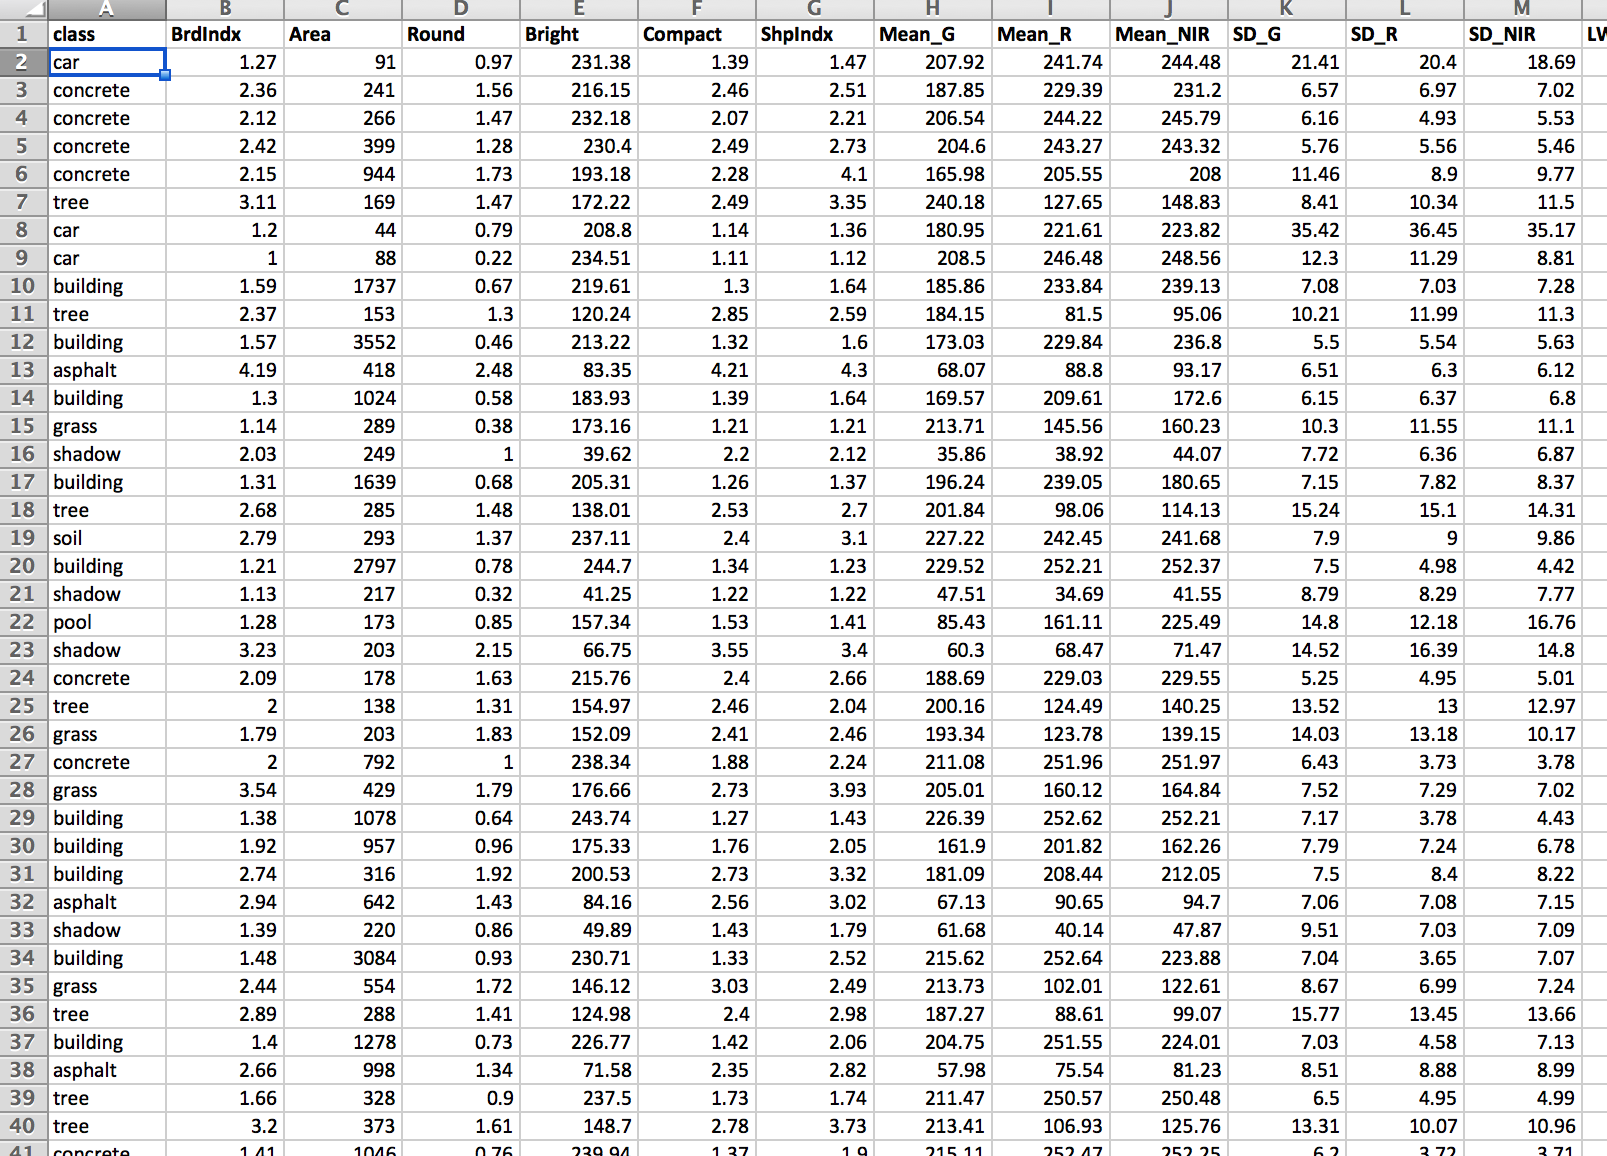
\includegraphics[width=0.7\linewidth]{_img/01-data} \end{center}

How do we make sense of all of these numbers and text? Visualising the
data can give us important insights into the underlying structure of the
data (covered in a previous workshop). The next step is to develop a
\textbf{model} that captures the salient features/structure of the data.

\section{What is a model?}\label{what-is-a-model}

\begin{quote}
A \textbf{model} is a human construct/abstraction that tries to
approximate the \textbf{data generating process} in some useful manner.
\end{quote}

Some people go even further:

\begin{quote}
Raw data, no matter how extensive, are useless without a model -
\href{https://www.newyorker.com/books/page-turner/what-nate-silver-gets-wrong\%22}{\textbf{Nate
Silver}}
\end{quote}

Models are built for various reasons:

\begin{itemize}
\tightlist
\item
  to enhance understanding of a complex phenomenon (e.g how does
  antibiotic resistance develop?);
\item
  to execute ``what if'' scenarios (e.g what happens if interest rates
  go up?);
\item
  to predict/forecast an outcome (e.g how many people will get influenza
  next winter?);
\item
  to control a system (e.g autonomous vehicles).
\end{itemize}

Models come in all kinds of ``languages'':

\begin{itemize}
\tightlist
\item
  a physical model e.g
  \href{https://www.anatomystuff.co.uk/clinical-skills-training-models.html}{medical
  training models}
\end{itemize}

\begin{center}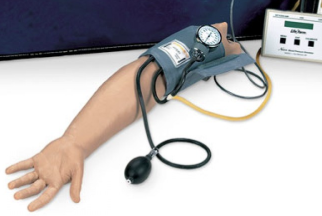
\includegraphics[width=0.45\linewidth]{_img/01-medical} \end{center}

\begin{itemize}
\tightlist
\item
  a verbal/pictorial model e.g
  \href{https://onlinelibrary.wiley.com/doi/pdf/10.1080/10739680701451516}{Francischetti
  \emph{et al. Microcirculation} (2008)}
\end{itemize}

\begin{center}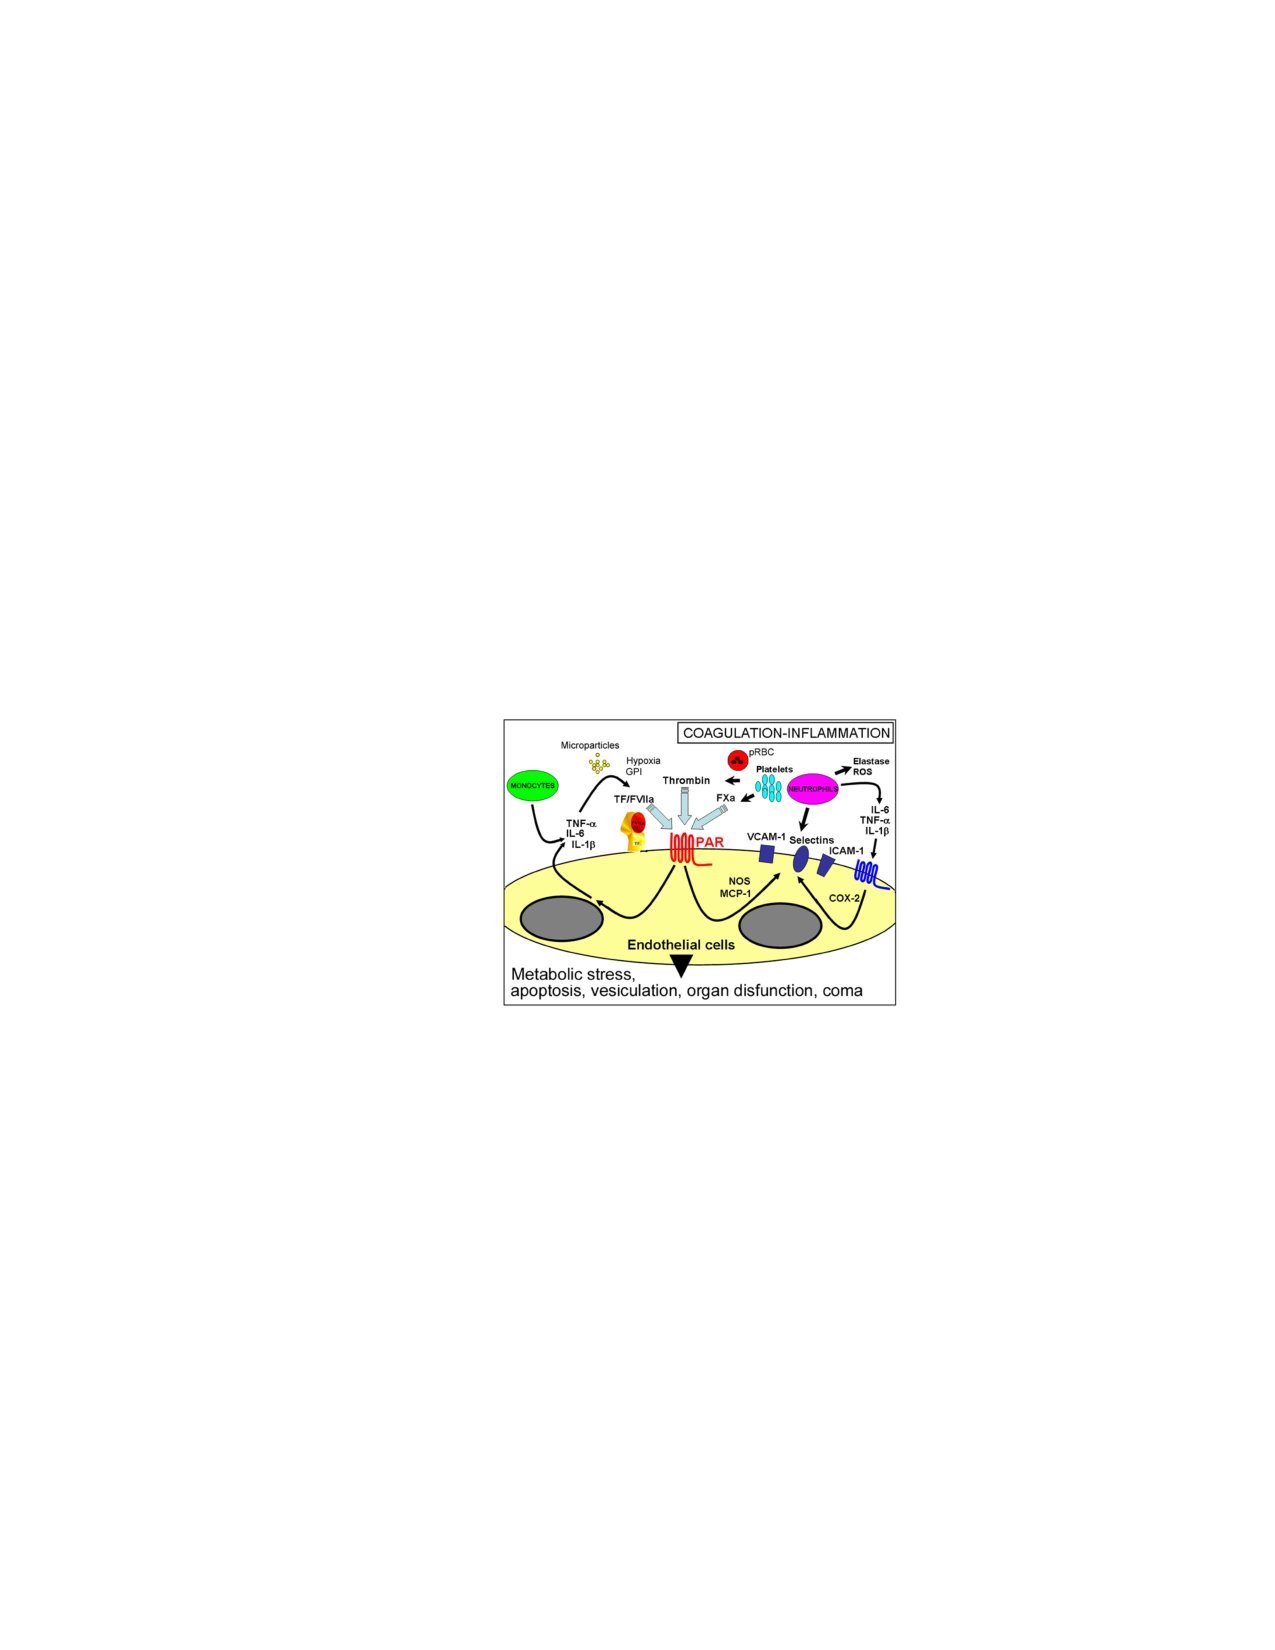
\includegraphics[width=0.5\linewidth]{_img/01-biological} \end{center}

\begin{itemize}
\tightlist
\item
  a mathematical model \[
  \begin{aligned}
  {\frac {\mathrm {d} x}{\mathrm {d} t}}& = \sigma (y-x),\\
  {\frac {\mathrm {d} y}{\mathrm {d} t}}& = x(\rho -z)-y\\
  {\frac {\mathrm {d} z}{\mathrm {d} t}}& = xy-\beta z
  \end{aligned}
  \]
\end{itemize}

\textbf{Assumptions} are an inherent part of every model; we cannot
build models if we are not prepared to make assumptions. The feasibility
of these assumptions is context-dependent but also on how the model will
be used.

Remember that models do \textbf{not} represent the real-world, they are
merely an ``abridged'' version of the real-world with many (many)
caveats!!

\begin{quote}
All models are wrong but some are useful - \textbf{George E.P. Box}
\end{quote}

\begin{quote}
For every complex question there is a simple and wrong solution -
\textbf{Albert Einstein}
\end{quote}

\section{What is a statistical (stochastic)
model?}\label{what-is-a-statistical-stochastic-model}

\begin{quote}
A \textbf{statistical model} is a mathematical model that makes a set of
statistical assumptions in the form of probability distributions (i.e we
assume that some variables follow a pre-defined probability
distribution).
\end{quote}

In this workshop we will solely focus on \textbf{linear} models. In
their simplest form these models can be used to fit ``straight lines''
(or hyperplanes; ``straight lines'' in higher dimensions) through data
points. However, this modelling framework is much more general, and can
model relationships between continuous and categorical variables, and
can also be used to fit curved relationships. So it provides a much
richer class of models than it first appears (though we will only focus
on simple cases in this workshop.)

\section{Illustrative example}\label{illustrative-example}

Remember when you used to run simple lab experiments at school and plot
data onto graph paper? It used to look something like this (with
different axes labels of course):

\begin{center}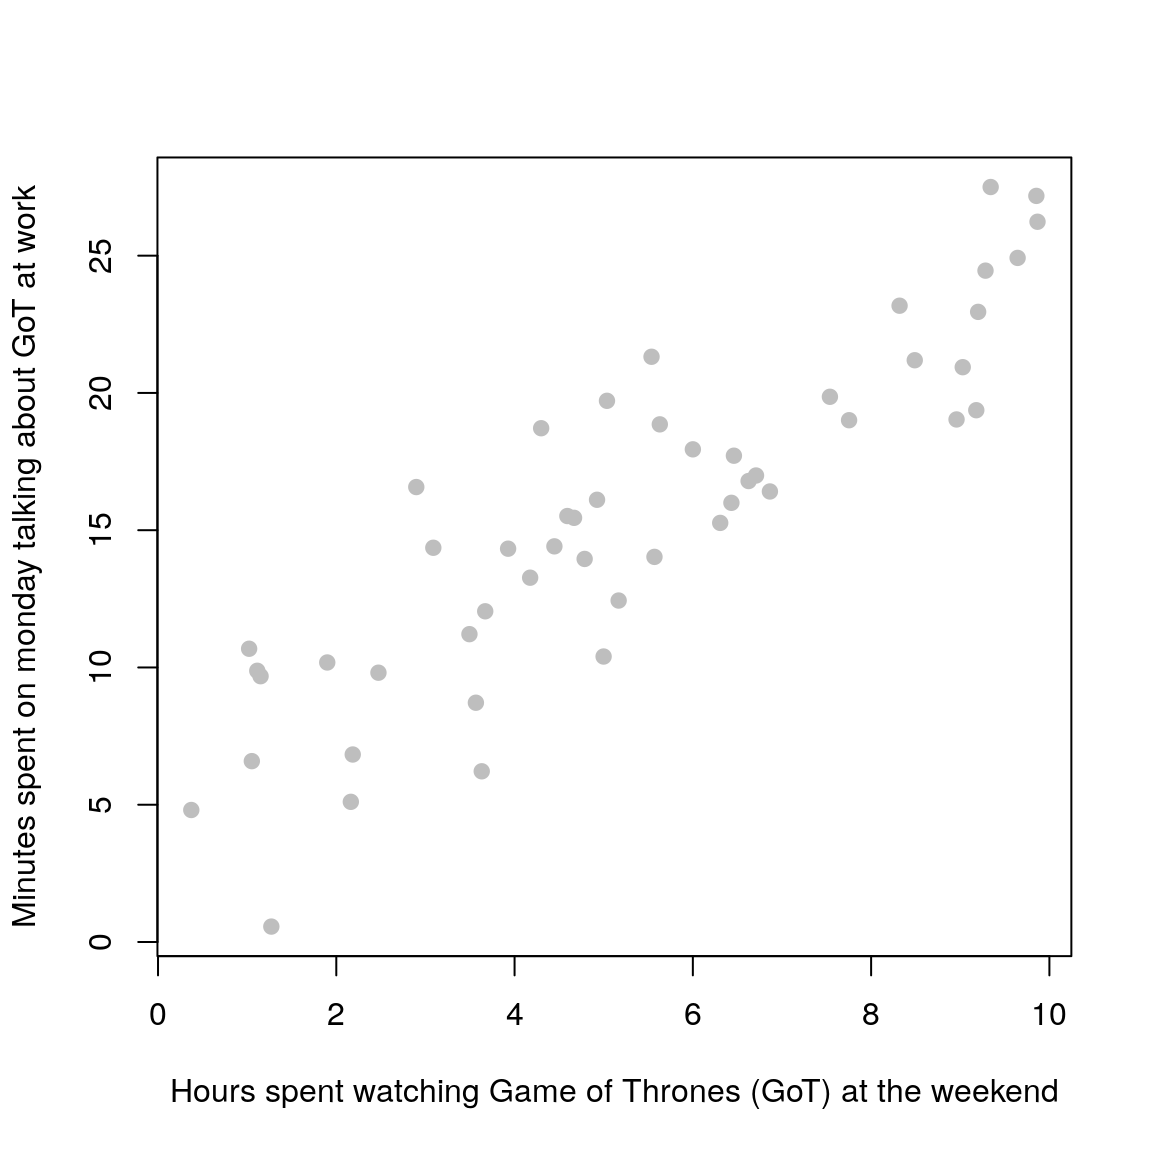
\includegraphics[width=0.6\linewidth]{_main_files/figure-latex/unnamed-chunk-6-1} \end{center}

Once you plotted out all of the data points, you were asked to grab a
ruler (a rigid, straight object) and find the line of best fit. To do
this, you used to try and get a roughly equal number of data points on
each side of the line.

\begin{center}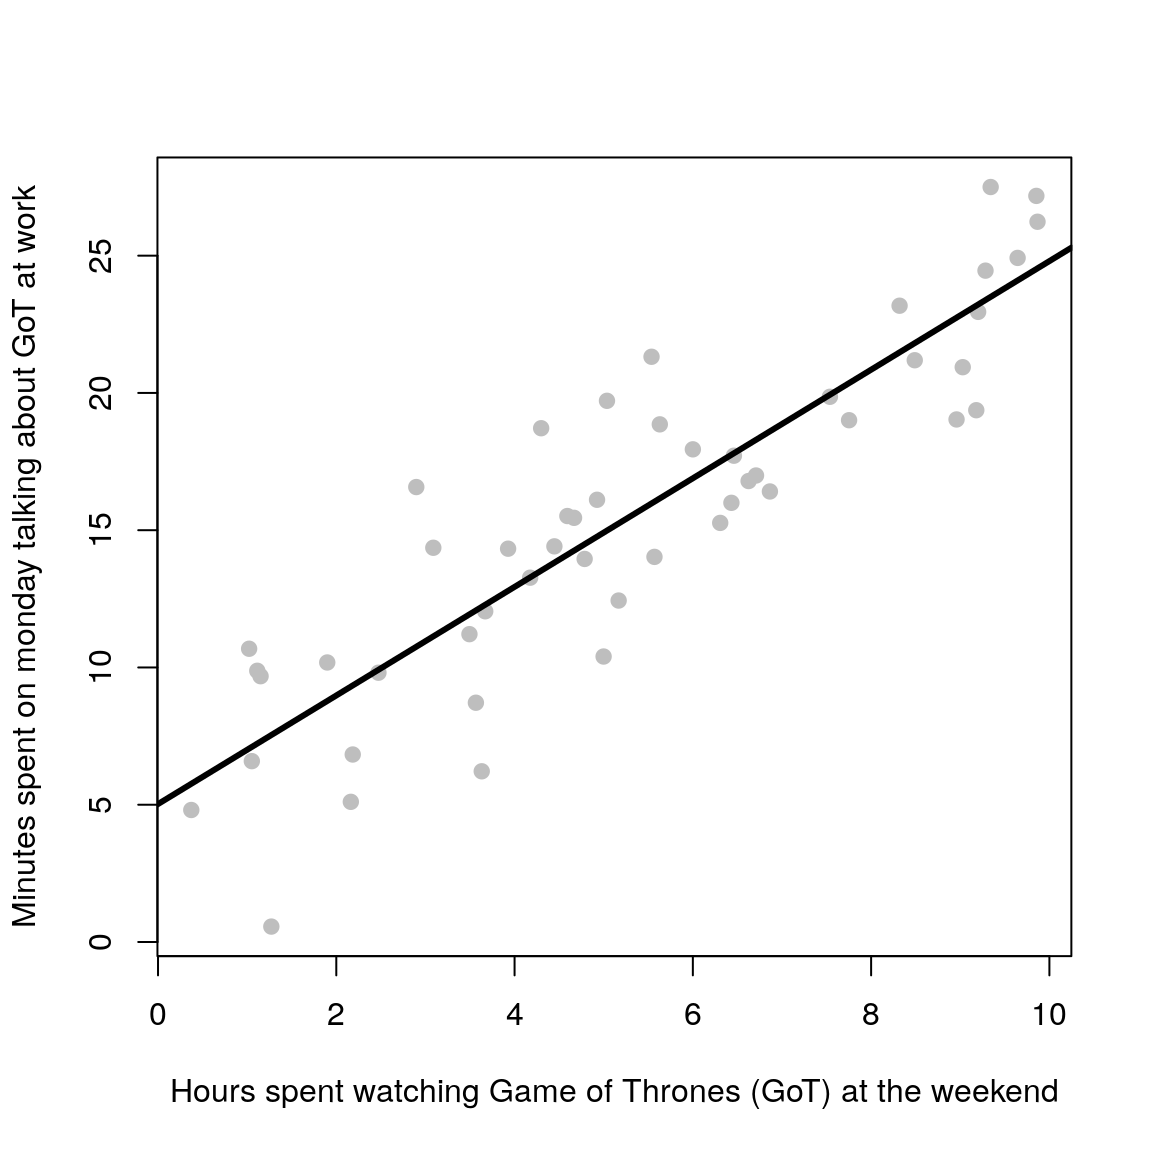
\includegraphics[width=0.6\linewidth]{_main_files/figure-latex/unnamed-chunk-7-1} \end{center}

\textbf{Congratulations!} Unknowingly, you were fitting a statistical
model to your measured data! Your best fit in that case was equivalent
to performing \textbf{ordinary least-squares} which minimises the
distance between the model (straight line) and your data points.

The fitted linear model is of the form \(y = mx + c\). Where \(m\) is
the gradient and \(c\) is the intercept (\(x\) is the dependent variable
and \(y\) the response variable i.e your measured data). At school you
were inferring the parameters \(m\) and \(c\) by hand. In this workshop
you will learn how to do it in R.

\begin{center}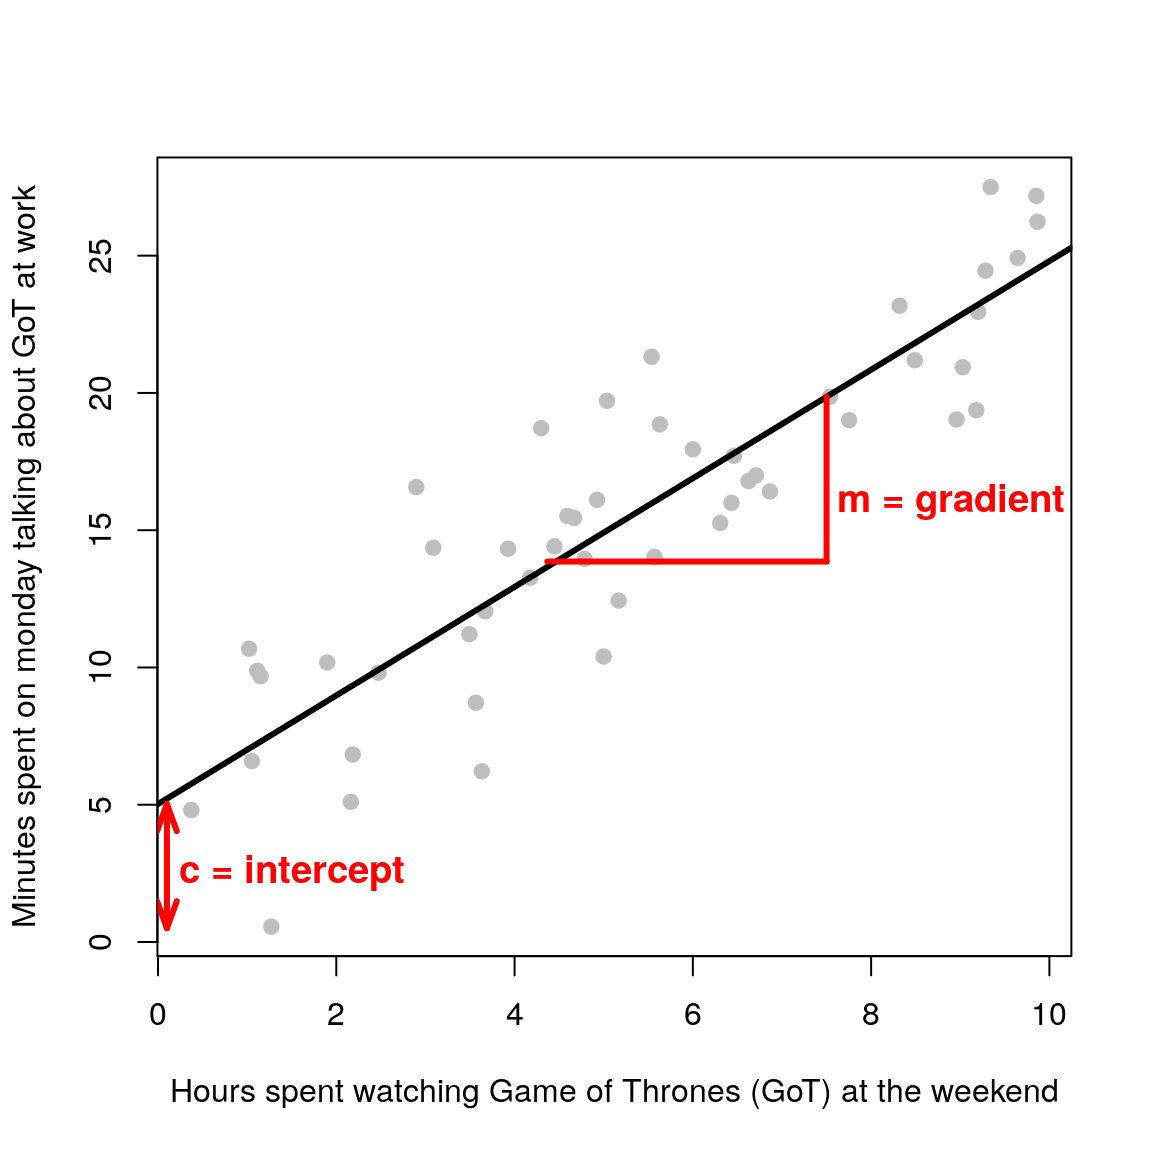
\includegraphics[width=0.6\linewidth]{_main_files/figure-latex/unnamed-chunk-8-1} \end{center}

What are the statistical assumptions in this case? As we will see in the
next chapter, in linear regression/modelling we assume that the
\textbf{residuals} i.e the differences between the model (black line)
and ``reality'' (observed data points), follow a
\href{https://en.wikipedia.org/wiki/Normal_distribution}{normal/Gaussian
distribution} (a bell curve).

\begin{center}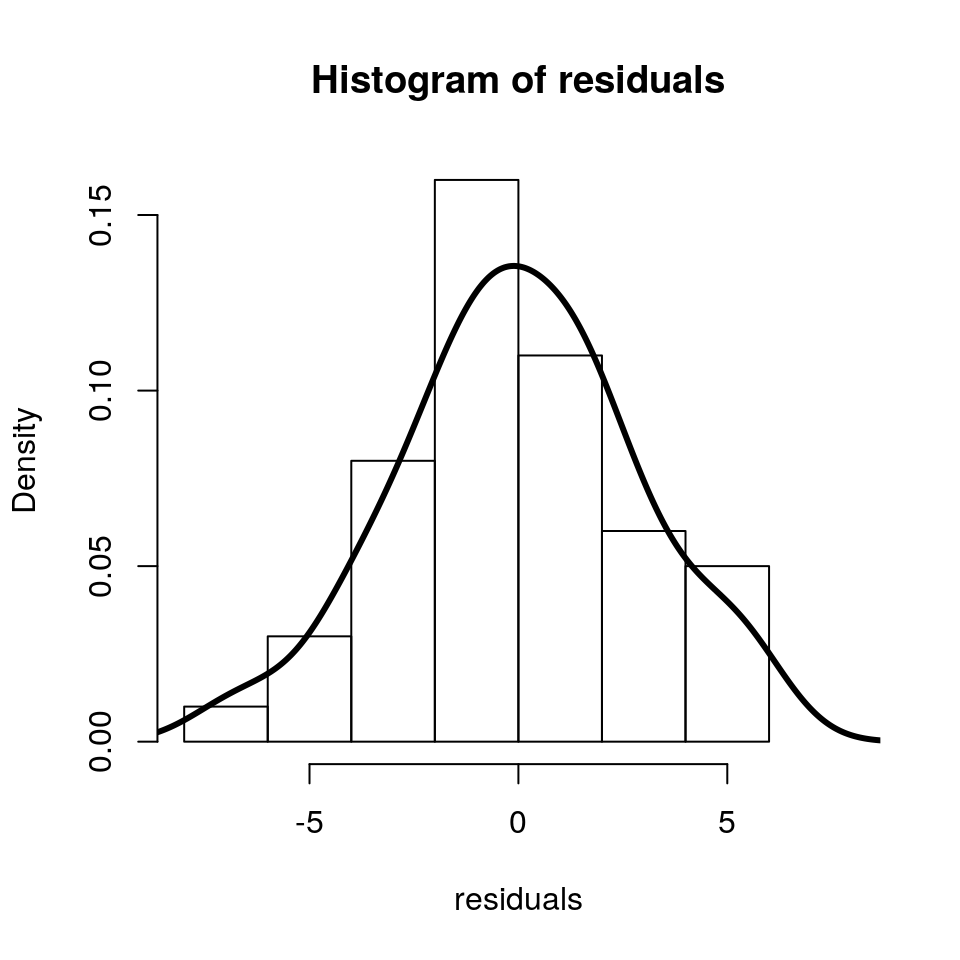
\includegraphics{_main_files/figure-latex/unnamed-chunk-9-1} \end{center}

\textbf{Model checking} involves confirming that our statistical
assumptions are sensible. We will delve into this in much detail later
on, but just remember that when you hear people saying ``check that your
data is normal'', in the context of linear regression, what this means
is that the \textbf{residuals} are normal (which also means that the
\textbf{response} variable is normal).

\section{Summary}\label{summary}

\begin{itemize}
\tightlist
\item
  Models are useful abstractions of the data that can help us understand
  the underlying system.
\item
  Linear regression is simply a flexible way to put a line-of-best-fit
  (or hyperplane) through the observed data points.
\item
  Model checking is the process of verifying the statistical assumptions
  made.
\end{itemize}

\chapter{Linear models}\label{linear-models}

Slides can be downloaded from:

\begin{itemize}
\tightlist
\item
  \href{https://exeter-data-analytics.github.io/StatModelling/02-linear-models-handout.pdf}{LMs
  in R}
\end{itemize}

\section{Simple linear regression}\label{simple-linear-regression}

In many scientific applications we are interested in exploring the
relationship between a single \textbf{response} variable and multiple
\textbf{explanatory} variables (predictors). We can do this by fitting a
linear model. Linear models \emph{per se} do not infer \emph{causality},
i.e defining a variable as response or explanatory is somewhat arbitrary
and depends on what the researcher is interested in. \emph{Causality}
can however be inferred through careful experimental design in a
well-controlled setting.

Consider again the case of one response and one explanatory variable.
From the previous chapter we know that this boils down to the equation
of a line (\(y = mx +c\)). Let's rename the parameters \(c\) and \(m\)
to \(\beta_0\) and \(\beta_1\), in line with statistical naming
convention\footnote{this notation is such that we can have any arbitrary
  large number of explantory variables i.e \(\beta_1\), \(\beta_2\),
  \(\beta_3\)\ldots{}etc., without running out of letters in the
  alphabet!}. It is just a change in name:

\[
\begin{aligned}
y = c + mx\\
y = \beta_0 + \beta_1x
\end{aligned}
\]

\begin{center}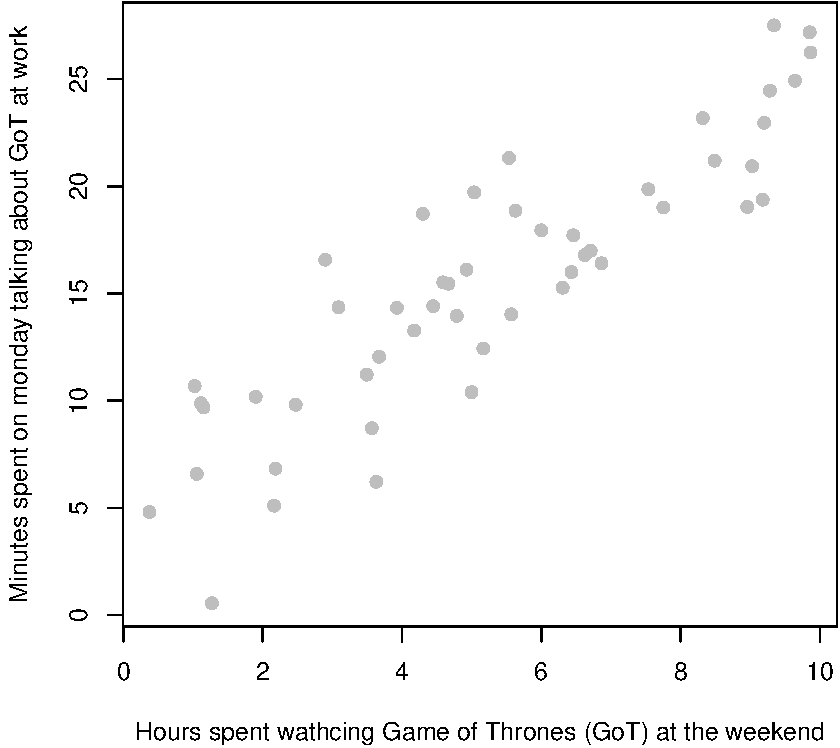
\includegraphics[width=0.6\linewidth]{_main_files/figure-latex/unnamed-chunk-11-1} \end{center}

Now suppose we measure \(n\) independent and identically distributed
(i.i.d) normally distributed outcomes \(y_1,\ldots,y_n\) (e.g height of
people) and we want to model their relationship with some explanatory
variable \(x\) (e.g weight of people). The linear regression model is
defined as follows:

\[
\begin{aligned}
y_i & = \beta_0 + \beta_1x_i + \epsilon_i \\
\epsilon_i & \sim \mathcal{N}(0, \sigma^2)
\end{aligned}
\] \(i\) is an index that goes from 1 to \(n\) (the total number of
observations). The equation is the same as before
(\(y = \beta_0 + \beta_1x\)), but now we have added an error term
\(\epsilon\). This term is needed because the straight line cannot go
through \emph{all} the data points (unless you have a very questionable
dataset)! It represents the discrepancy between the model (the fitted
straight line) and the observed data (grey points).

\(\epsilon\) is also known as the \textbf{noise} term. The reason is
that in general our response variable has some uncertainty associated
with it (e.g counting the number of birds in an area, quantifying gene
expression using microarrays or RNA-seq, etc.). The statistical
assumption in linear modelling is that these errors are normally
distributed with mean zero and some standard deviation \(\sigma\)
(mathematically this is written as
\(\epsilon_i \sim \mathcal{N}(0, \sigma^2)\)). This means that the
\textbf{response} variable is also assumed to be normally distributed.
For the maths aficionados amongst you:

\[
y_i \sim \mathcal{N}(\beta_0 + \beta_1x_i, \sigma^2)
\] Note that we do not make explicit assumptions about the
\textbf{explanatory} variables (the \(x\)'s) i.e they don't need to be
normal.

The workflow in linear regression is as follows:

\begin{enumerate}
\def\labelenumi{\arabic{enumi}.}
\tightlist
\item
  Infer the model's parameters \(\beta_0\) and \(\beta_1\).
\item
  Check the model fit.
\item
  Interpret the \textbf{practical} significance of the estimated
  parameters.
\end{enumerate}

\section{Doing it in R}\label{doing-it-in-r}

Luckily for us, we do not need to worry about the mathematical
intricacies of estimating the model's parameters, R will do it for us.
Let's generate some fake data just to get things started.

\begin{Shaded}
\begin{Highlighting}[]
\KeywordTok{set.seed}\NormalTok{(}\DecValTok{1453}\NormalTok{)}
\NormalTok{N <-}\StringTok{ }\DecValTok{100}\NormalTok{ ## no. of observations}
\NormalTok{weight <-}\StringTok{ }\KeywordTok{runif}\NormalTok{(}\DataTypeTok{n=}\NormalTok{N, }\DataTypeTok{min=}\DecValTok{60}\NormalTok{, }\DataTypeTok{max=}\DecValTok{100}\NormalTok{) ## hypothetical weights in kg}
\NormalTok{height <-}\StringTok{ }\FloatTok{2.2}\OperatorTok{*}\NormalTok{weight }\OperatorTok{+}\StringTok{ }\KeywordTok{rnorm}\NormalTok{(}\DataTypeTok{n=}\NormalTok{N, }\DataTypeTok{mean=}\DecValTok{0}\NormalTok{, }\DataTypeTok{sd=}\DecValTok{10}\NormalTok{) ## hypothetical heights in cm}
\KeywordTok{plot}\NormalTok{(weight, height, }\DataTypeTok{pch=}\DecValTok{19}\NormalTok{, }\DataTypeTok{xlab=}\StringTok{'Weight (kg)'}\NormalTok{, }\DataTypeTok{ylab=}\StringTok{'Height (cm)'}\NormalTok{, }\DataTypeTok{col=}\StringTok{'grey'}\NormalTok{)}
\end{Highlighting}
\end{Shaded}

\begin{center}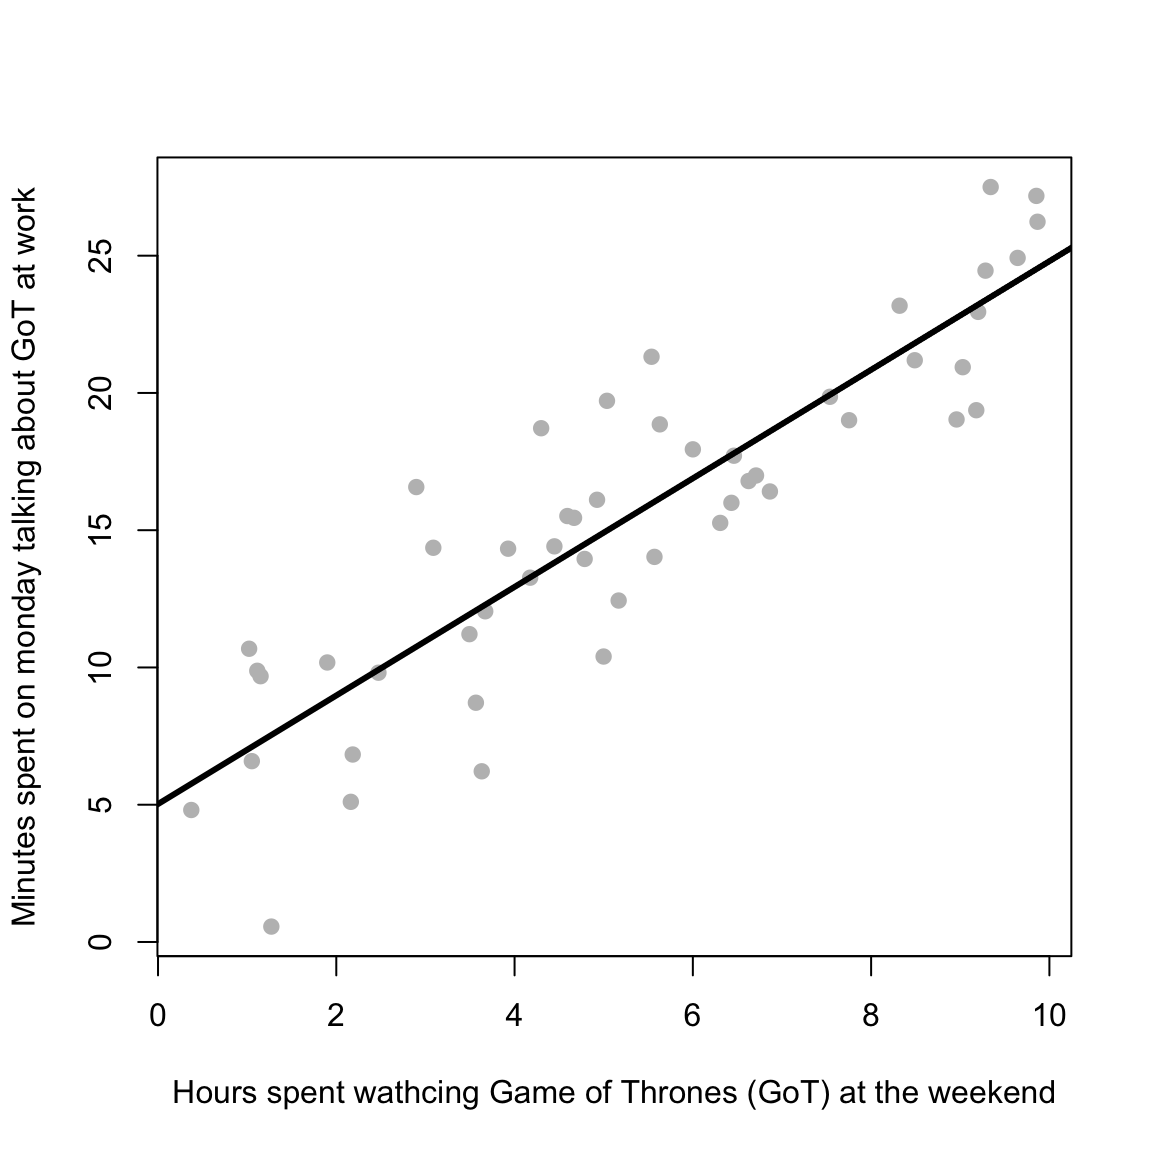
\includegraphics[width=0.6\linewidth]{_main_files/figure-latex/unnamed-chunk-12-1} \end{center}

To fit a linear model we use the
\href{https://www.rdocumentation.org/packages/stats/versions/3.5.1/topics/lm}{\texttt{lm()}}
function (\textbf{always} read the documentation of a function before
using it!). This function requires a \textbf{formula} object which has
the form of \texttt{response\ \textasciitilde{}\ explanatory}. So in our
case this will be \texttt{height\ \textasciitilde{}\ weight}. R will
then fit the following model \footnote{weight is our explanatory
  variable (\(x_i\)) and height the response variable (\(y_i\))}:

\[
\mathrm{height}_i = \beta_0 + \beta_1\mathrm{weight}_i + \epsilon_i
\] Let's call the R function, plot the model fit and print the output.

\begin{Shaded}
\begin{Highlighting}[]
\NormalTok{## Linear model fit}
\NormalTok{fit <-}\StringTok{ }\KeywordTok{lm}\NormalTok{(height }\OperatorTok{~}\StringTok{ }\NormalTok{weight)}

\NormalTok{## Plot model fit}
\KeywordTok{plot}\NormalTok{(weight, height, }\DataTypeTok{pch=}\DecValTok{19}\NormalTok{, }\DataTypeTok{xlab=}\StringTok{'Weight (kg)'}\NormalTok{, }\DataTypeTok{ylab=}\StringTok{'Height (cm)'}\NormalTok{, }\DataTypeTok{col=}\StringTok{'grey'}\NormalTok{)}
\KeywordTok{lines}\NormalTok{(weight, }\KeywordTok{predict}\NormalTok{(fit), }\DataTypeTok{col=}\StringTok{'black'}\NormalTok{, }\DataTypeTok{lwd=}\DecValTok{3}\NormalTok{)}
\end{Highlighting}
\end{Shaded}

\begin{center}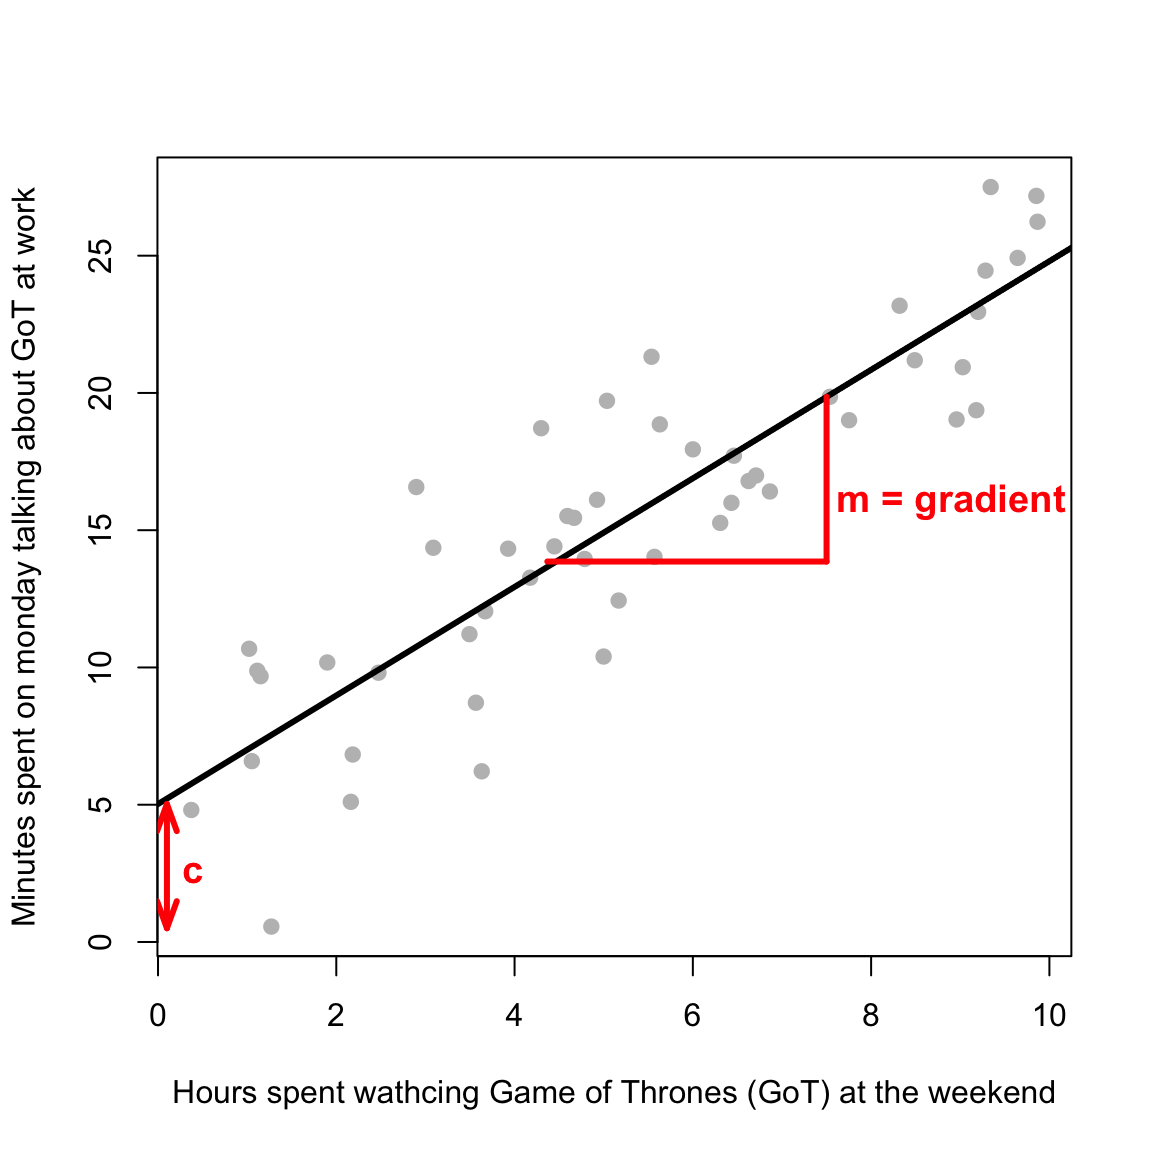
\includegraphics[width=0.6\linewidth]{_main_files/figure-latex/unnamed-chunk-13-1} \end{center}

\begin{Shaded}
\begin{Highlighting}[]
\NormalTok{## Print result}
\KeywordTok{print}\NormalTok{(fit)}
\end{Highlighting}
\end{Shaded}

\begin{verbatim}
## 
## Call:
## lm(formula = height ~ weight)
## 
## Coefficients:
## (Intercept)       weight  
##       2.352        2.174
\end{verbatim}

This outputs two numbers, the \texttt{(Intercept)=} 2.352 cm and
\texttt{weight=} 2.174 cm/kg. These are the \(\beta_0\) and \(\beta_1\)
parameters.

The \(\beta_0\) parameter (intercept) is not very useful in this case,
it basically tells us what's the expected height of someone that weighs
0 kg (2.352 cm here). This is of course nonsense, but I'm highlighting
it as a reminder that the assumptions that underlie these models can
only be tested within the range of the observed data.

\begin{quote}
\textbf{Aside}: using the model to predict outside of the range of the
observed data is called \textbf{extrapolating}. Oftentimes, statistical
models are developed \emph{in order} to be used to extrapolate
(e.g.~climate modelling). This is however, dangerous, as we can only
assess the assumptions of the model over the range of the observed data.
When extrapolating we have to assume that these relationships hold
beyond the range of the data, which may or may not be reasonable (hence
why weather forecast over short-time periods are OK, but climate
forecasts are much more uncertain). Hence, we should always view the
model as an approximation of the data generating process. In this
particualr case, the interpretation of the parameters is not sensible
when \(x = 0\) (weight = 0 kg), but makes sense in the range that we are
interested in exploring. If the case where \(x = 0\) is important, then
we would have to change the model to ensure that the predictions made
sense at those values of \(x\).
\end{quote}

The \(\beta_1\) parameter (gradient) tells us about the relationship
between the outcome and explanatory variable. In this case, for every 1
kg increase in weight on \emph{average} the height increases by 2.174
cm.

\begin{quote}
\textbf{Warning}: the notation used by R can come across as confusing.
Although the returned value is labelled as \texttt{weight}, in fact it
corresponds to the \(\beta_1\) parameter that relates to the strength of
linear relationship between \texttt{weight} and \texttt{height} (i.e it
is a gradient).
\end{quote}

\subsection{Using data frames}\label{using-data-frames}

The \texttt{lm()} function also accepts \textbf{data frames} as input
arguments.

\begin{Shaded}
\begin{Highlighting}[]
\NormalTok{## Create data frame}
\NormalTok{df <-}\StringTok{ }\KeywordTok{data.frame}\NormalTok{(}\DataTypeTok{height=}\NormalTok{height, }\DataTypeTok{weight=}\NormalTok{weight)}
\KeywordTok{head}\NormalTok{(df)}
\end{Highlighting}
\end{Shaded}

\begin{verbatim}
##     height   weight
## 1 211.9054 86.59694
## 2 178.6420 77.28891
## 3 206.1585 95.01870
## 4 157.4803 70.66759
## 5 175.6296 79.84837
## 6 176.1113 83.98290
\end{verbatim}

\begin{Shaded}
\begin{Highlighting}[]
\NormalTok{## Fit linear model}
\NormalTok{fit <-}\StringTok{ }\KeywordTok{lm}\NormalTok{(height }\OperatorTok{~}\StringTok{ }\NormalTok{weight, }\DataTypeTok{data=}\NormalTok{df)}
\end{Highlighting}
\end{Shaded}

\subsection{Extended summary}\label{extended-summary}

The object returned by \texttt{lm()} contains further information that
we can display using the \texttt{summary()} function.

\begin{Shaded}
\begin{Highlighting}[]
\KeywordTok{summary}\NormalTok{(fit)}
\end{Highlighting}
\end{Shaded}

\begin{verbatim}
## 
## Call:
## lm(formula = height ~ weight, data = df)
## 
## Residuals:
##     Min      1Q  Median      3Q     Max 
## -31.089  -6.926  -0.689   6.057  24.967 
## 
## Coefficients:
##             Estimate Std. Error t value Pr(>|t|)    
## (Intercept)  2.35229    7.11668   0.331    0.742    
## weight       2.17446    0.08782  24.762   <2e-16 ***
## ---
## Signif. codes:  0 '***' 0.001 '**' 0.01 '*' 0.05 '.' 0.1 ' ' 1
## 
## Residual standard error: 10.31 on 98 degrees of freedom
## Multiple R-squared:  0.8622, Adjusted R-squared:  0.8608 
## F-statistic: 613.1 on 1 and 98 DF,  p-value: < 2.2e-16
\end{verbatim}

That's a lot of information, let's unpick it line by line:

\begin{itemize}
\item
  \textbf{Call}

  This just states the arguments that were passed to the \texttt{lm()}
  function. Remember it's
  \texttt{response\ \textasciitilde{}\ explanatory}.
\end{itemize}

\newpage

\begin{itemize}
\item
  \textbf{Residuals}

  Some basic stats about the residuals (i.e the differences between the
  model fit and the observed data points). It is easier to plot a
  histogram of the residuals (shown in the next section), but these
  basic stats can already give us an indication of whether we have a
  symmetric distribution with zero mean (i.e we want the median to be
  close to zero, the third quartile (3Q) to be roughly equal to -1Q
  (first quartile) and the max to be approximately -min).
\item
  \textbf{Coefficients}

  \begin{itemize}
  \tightlist
  \item
    \textbf{\texttt{Estimate}}
  \end{itemize}

  The \texttt{(Intercept)=} 2.352 cm and \texttt{weight=} 2.174 cm/kg
  are the \(\beta_0\) and \(\beta_1\) parameters as discussed earlier.

  \begin{itemize}
  \tightlist
  \item
    \textbf{\texttt{Std.\ Error}}
  \end{itemize}

  The standard error for that parameter. It tells us how confident we
  are in estimating that particular parameter. If the standard error is
  comparable or greater than the actual parameter estimate itself then
  that point estimate should not be trusted. We can also show the
  confidence intervals for the model parameters to highlight their
  uncertainty using the \texttt{confint()} function:

\begin{Shaded}
\begin{Highlighting}[]
\KeywordTok{confint}\NormalTok{(fit, }\DataTypeTok{level=}\FloatTok{0.97}\NormalTok{) ## pick the 97% confidence intervals}
\end{Highlighting}
\end{Shaded}

\begin{verbatim}
##                  1.5 %    98.5 %
## (Intercept) -13.319698 18.024268
## weight        1.981077  2.367844
\end{verbatim}

  \begin{itemize}
  \tightlist
  \item
    \textbf{\texttt{t\ value}} and
    \textbf{\texttt{Pr(\textgreater{}\textbar{}t\textbar{})}}
  \end{itemize}

  This is the result of a hypothesis testing against the null hypothesis
  that the coefficient is zero.
\item
  \textbf{Residual standard error}

  The square root of residual sum of squares/degress of freedom

\begin{Shaded}
\begin{Highlighting}[]
\NormalTok{## Residual standard error}
\KeywordTok{sqrt}\NormalTok{(}\KeywordTok{sum}\NormalTok{(}\KeywordTok{residuals}\NormalTok{(fit)}\OperatorTok{^}\DecValTok{2}\NormalTok{) }\OperatorTok{/}\StringTok{ }\NormalTok{fit}\OperatorTok{$}\NormalTok{df.residual) }
\end{Highlighting}
\end{Shaded}

\begin{verbatim}
## [1] 10.31254
\end{verbatim}
\item
  \textbf{Multiple R-squared}

  Total variation = \textbf{Regression} (explained) variation +
  \textbf{Residual} (unexplained) variation

  The \(R^2\) statistic (also known as the \textbf{coefficient of
  determination}) is the proportion of the total variation that is
  explained by the regression. In regression with a single explanatory
  variable, this is the same as the Pearson correlation coefficient
  squared:

\begin{Shaded}
\begin{Highlighting}[]
\KeywordTok{cor}\NormalTok{(height, weight)}\OperatorTok{^}\DecValTok{2}
\end{Highlighting}
\end{Shaded}

\begin{verbatim}
## [1] 0.8621921
\end{verbatim}
\item
  \textbf{F-statistic}

  \[
  \text{F-statistic} = \frac{\text{Regression (explained) variation}}{\text{Residual (unexplained) variation}}
  \]

  The F-statistic can be used to assess whether the amount of variation
  explained by the regression (\(M_1\)) is \emph{statistically
  significantly} different compared to the \textbf{null} model (\(M_0\)
  - in this case the \textbf{null} model is the same as just taking the
  mean of the data). Large values of the F-statistic correspond to cases
  where the model fit is better for the more complex model compared to
  the null model. This test can be used to generate a p-value to assess
  whether the model fit is statistically significantly better given a
  pre-defined level of significance.

  \[
  \begin{aligned}
  M_0:~~~~~y_i &= \beta_0 + \epsilon_i\\  
  M_1:~~~~~y_i &= \beta_0 + \beta_1 W_i + \epsilon_i
  \end{aligned}
  \]
\end{itemize}

\section{Model checking}\label{model-checking}

The extended summary leads us nicely to the concept of model checking.
In theory, we can fit an infinite number of different models to the same
data by placing different assumptions/constraints. Recall:

\begin{quote}
All models are wrong but some are useful - \textbf{George E.P. Box}
\end{quote}

In order to make \textbf{robust} inference, we must \textbf{check} the
model fit

Model checking boils down to confirming whether or not the assumptions
that we have placed on the model are reasonable. Our main assumption is
that the residuals are normally distributed centred around zero. Let's
plot this:

\begin{Shaded}
\begin{Highlighting}[]
\KeywordTok{hist}\NormalTok{(fit}\OperatorTok{$}\NormalTok{residuals)}
\end{Highlighting}
\end{Shaded}

\begin{center}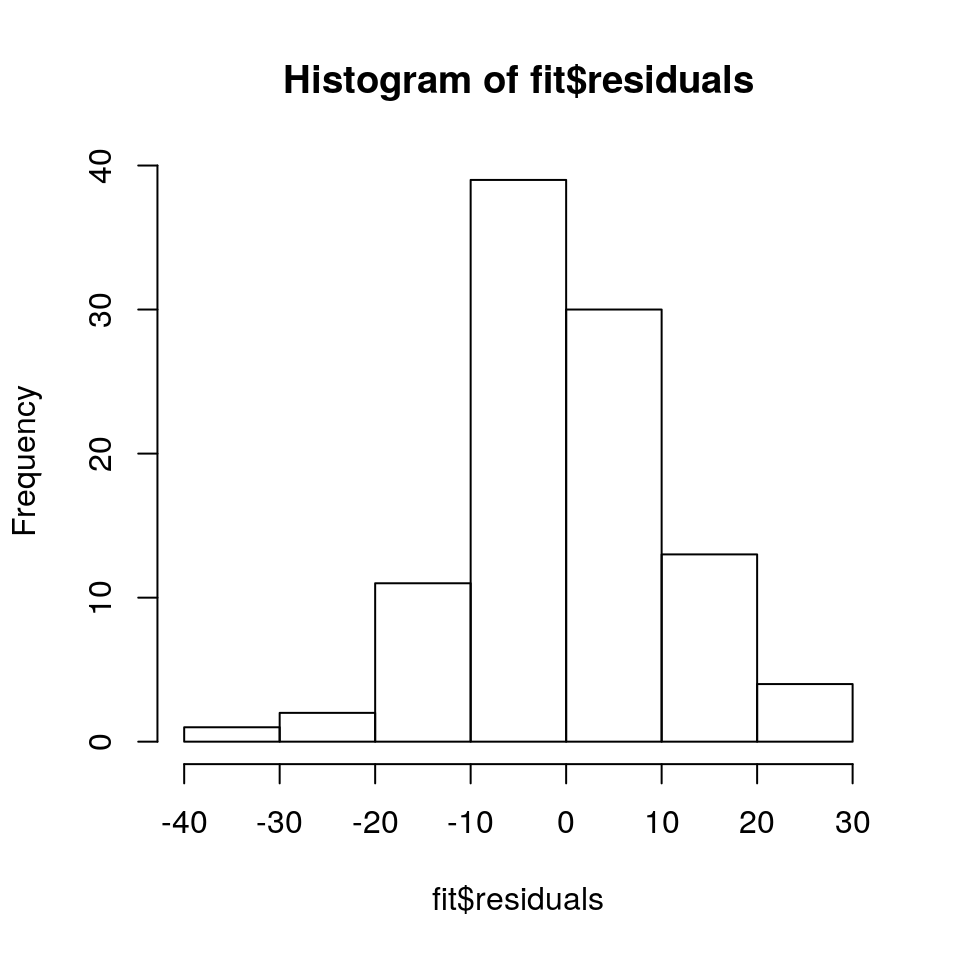
\includegraphics{_main_files/figure-latex/unnamed-chunk-19-1} \end{center}

The residuals are fairly normally distributed which is a good sign. R
also provides us with the following diagnostic plots:

\begin{Shaded}
\begin{Highlighting}[]
\KeywordTok{par}\NormalTok{(}\DataTypeTok{mfrow=}\KeywordTok{c}\NormalTok{(}\DecValTok{2}\NormalTok{, }\DecValTok{2}\NormalTok{))}
\KeywordTok{plot}\NormalTok{(fit, }\DataTypeTok{pch=}\DecValTok{19}\NormalTok{, }\DataTypeTok{col=}\StringTok{'darkgrey'}\NormalTok{)}
\end{Highlighting}
\end{Shaded}

\begin{center}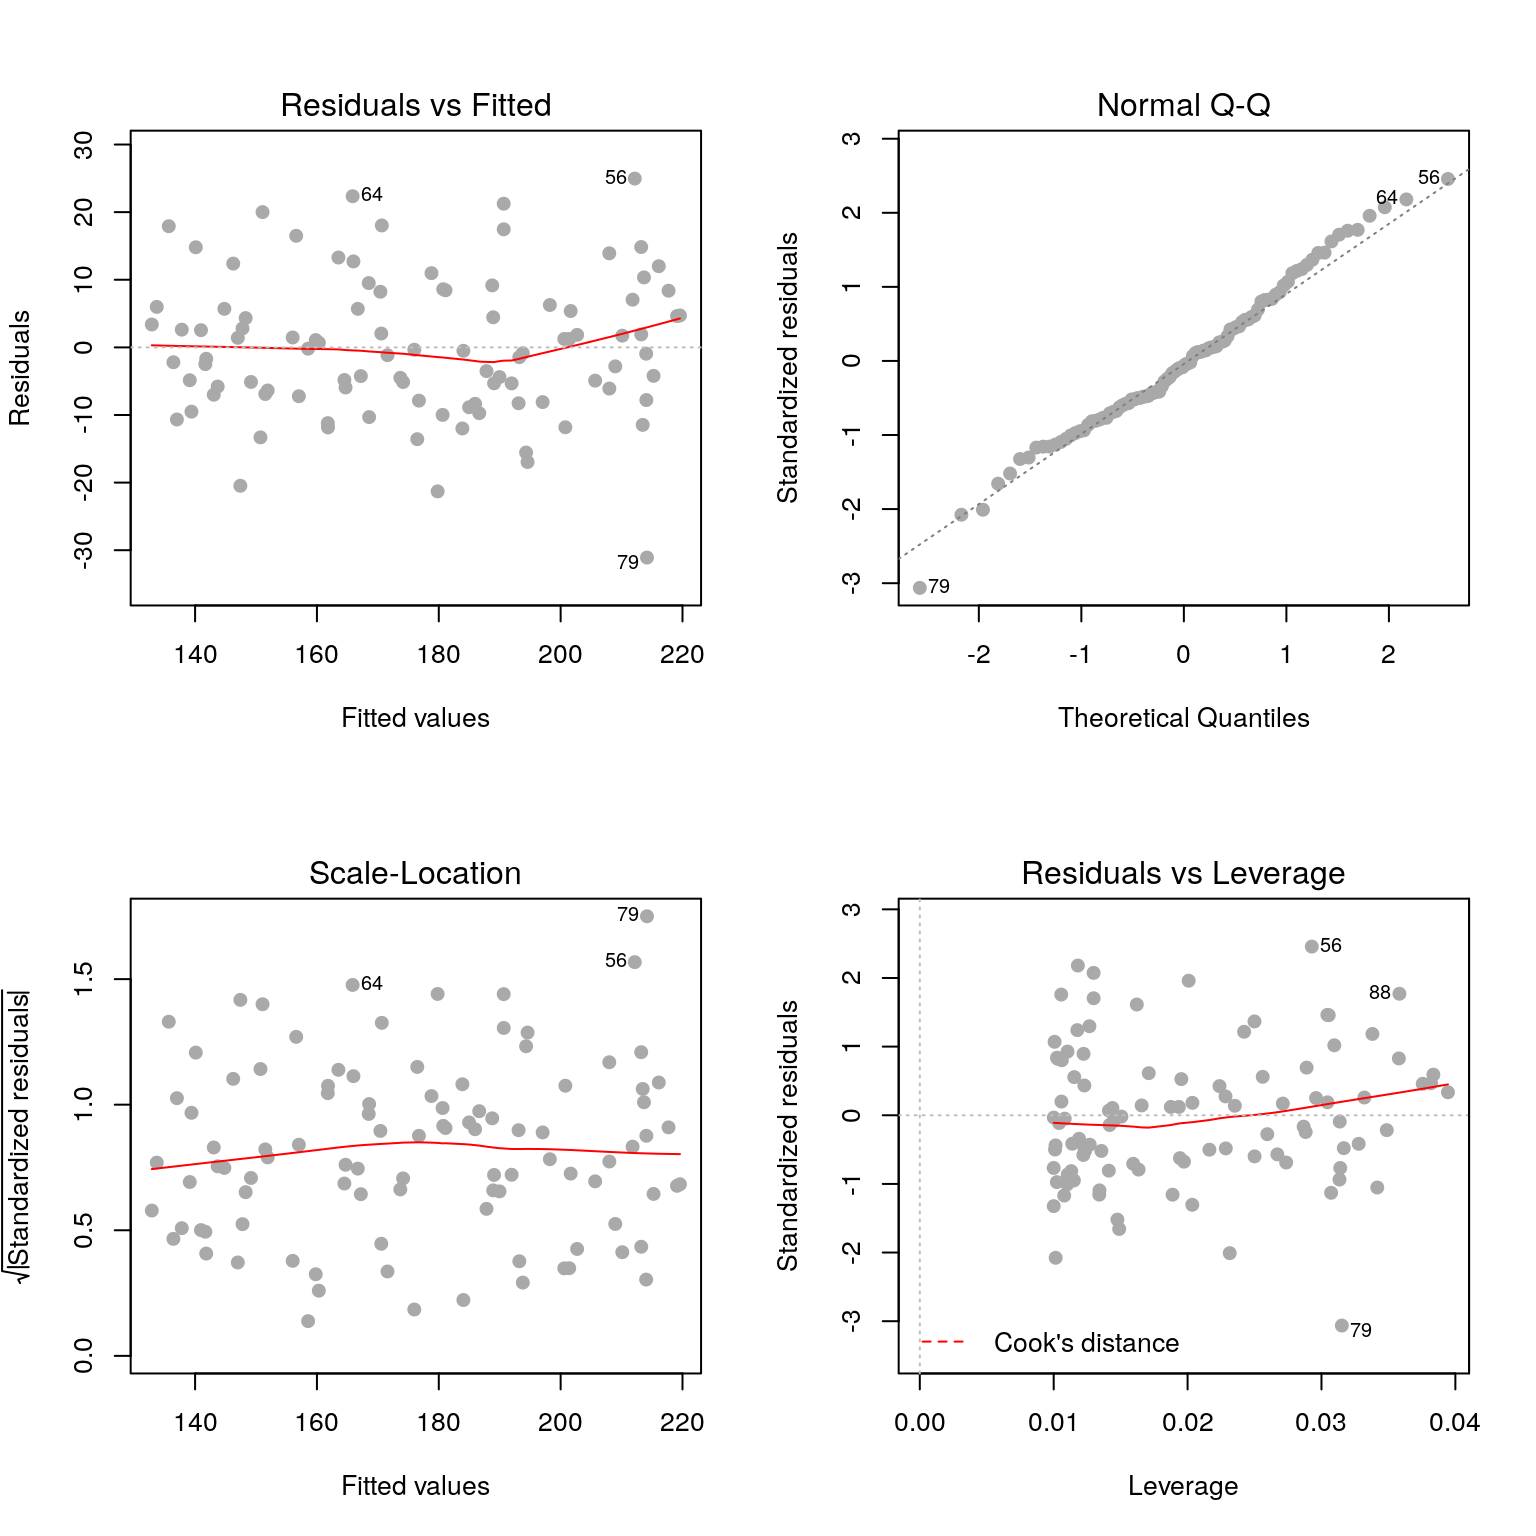
\includegraphics{_main_files/figure-latex/unnamed-chunk-20-1} \end{center}

\subsection{Residuals vs fitted
values}\label{residuals-vs-fitted-values}

\begin{Shaded}
\begin{Highlighting}[]
\KeywordTok{plot}\NormalTok{(fit, }\DataTypeTok{pch=}\DecValTok{19}\NormalTok{, }\DataTypeTok{col=}\StringTok{'darkgrey'}\NormalTok{, }\DataTypeTok{which=}\DecValTok{1}\NormalTok{)}
\end{Highlighting}
\end{Shaded}

\begin{center}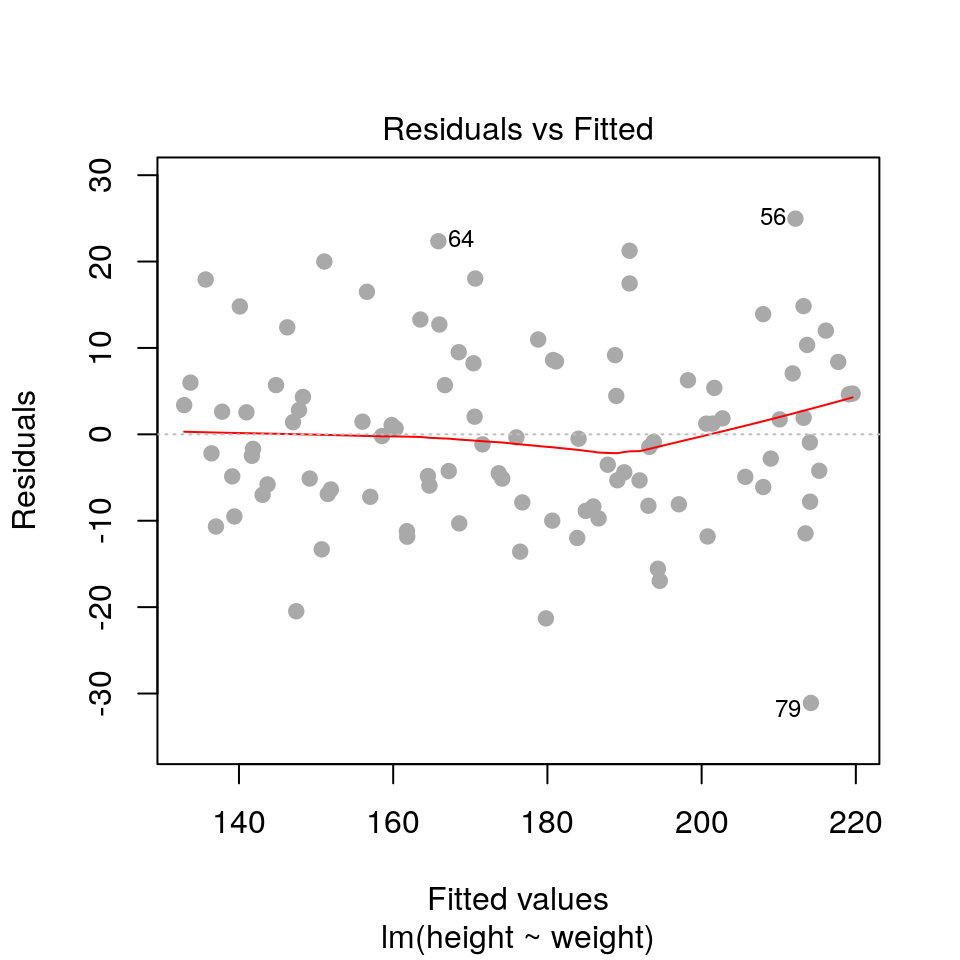
\includegraphics{_main_files/figure-latex/unnamed-chunk-22-1} \end{center}

Here we are checking that the variance is constant along the fitted
line\footnote{non-constant variance is known as \textbf{heteroscedacity}},
and that there are no systematic patterns in the residuals.

A couple of example where this assumption is violated.

\begin{center}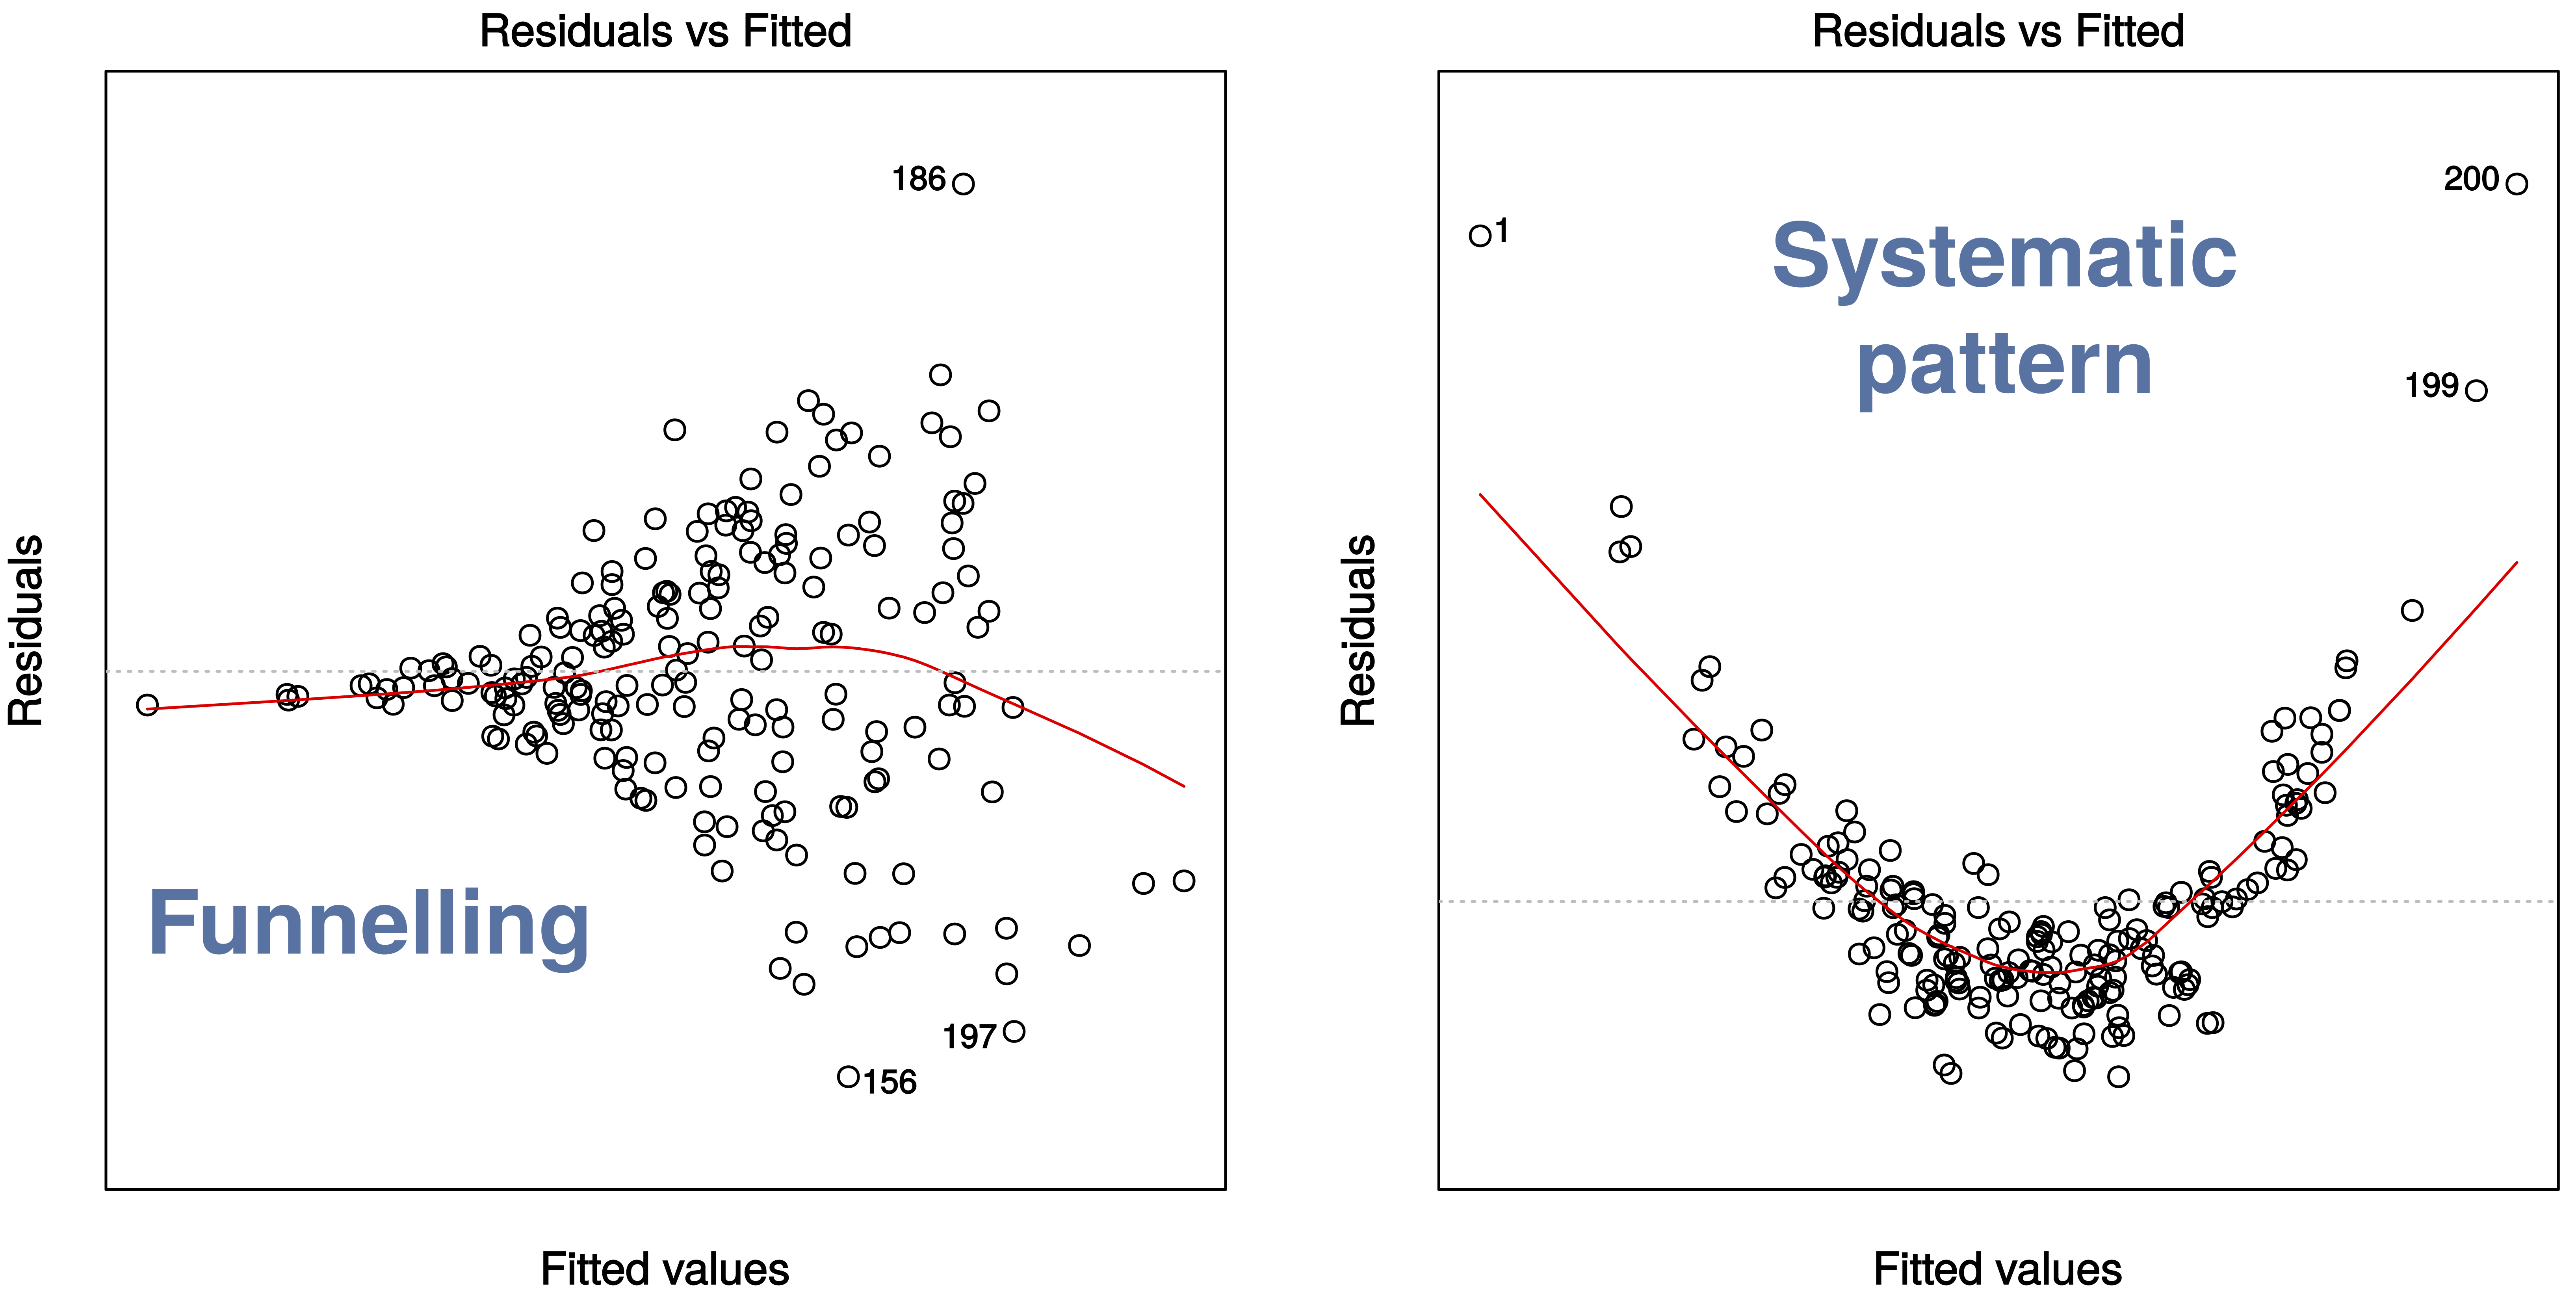
\includegraphics[width=0.9\linewidth]{_img/02-funnel} \end{center}

\subsection{Residuals vs fitted values
(scale-location)}\label{residuals-vs-fitted-values-scale-location}

\begin{Shaded}
\begin{Highlighting}[]
\KeywordTok{plot}\NormalTok{(fit, }\DataTypeTok{pch=}\DecValTok{19}\NormalTok{, }\DataTypeTok{col=}\StringTok{'darkgrey'}\NormalTok{, }\DataTypeTok{which=}\DecValTok{3}\NormalTok{)}
\end{Highlighting}
\end{Shaded}

\begin{center}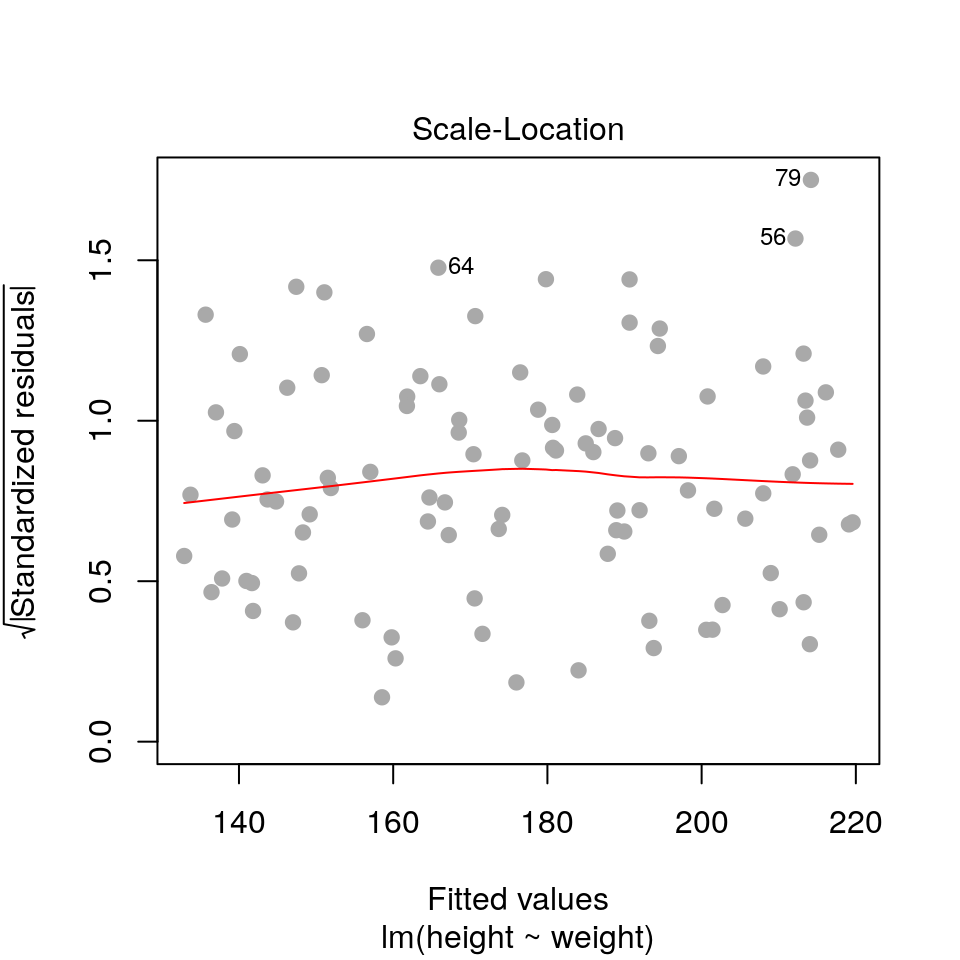
\includegraphics{_main_files/figure-latex/unnamed-chunk-24-1} \end{center}

This is similar to the first plot but on a different scale.

\newpage

\subsection{Residuals vs.~leverage}\label{residuals-vs.leverage}

\begin{Shaded}
\begin{Highlighting}[]
\KeywordTok{plot}\NormalTok{(fit, }\DataTypeTok{pch=}\DecValTok{19}\NormalTok{, }\DataTypeTok{col=}\StringTok{'darkgrey'}\NormalTok{, }\DataTypeTok{which=}\DecValTok{5}\NormalTok{)}
\end{Highlighting}
\end{Shaded}

\begin{center}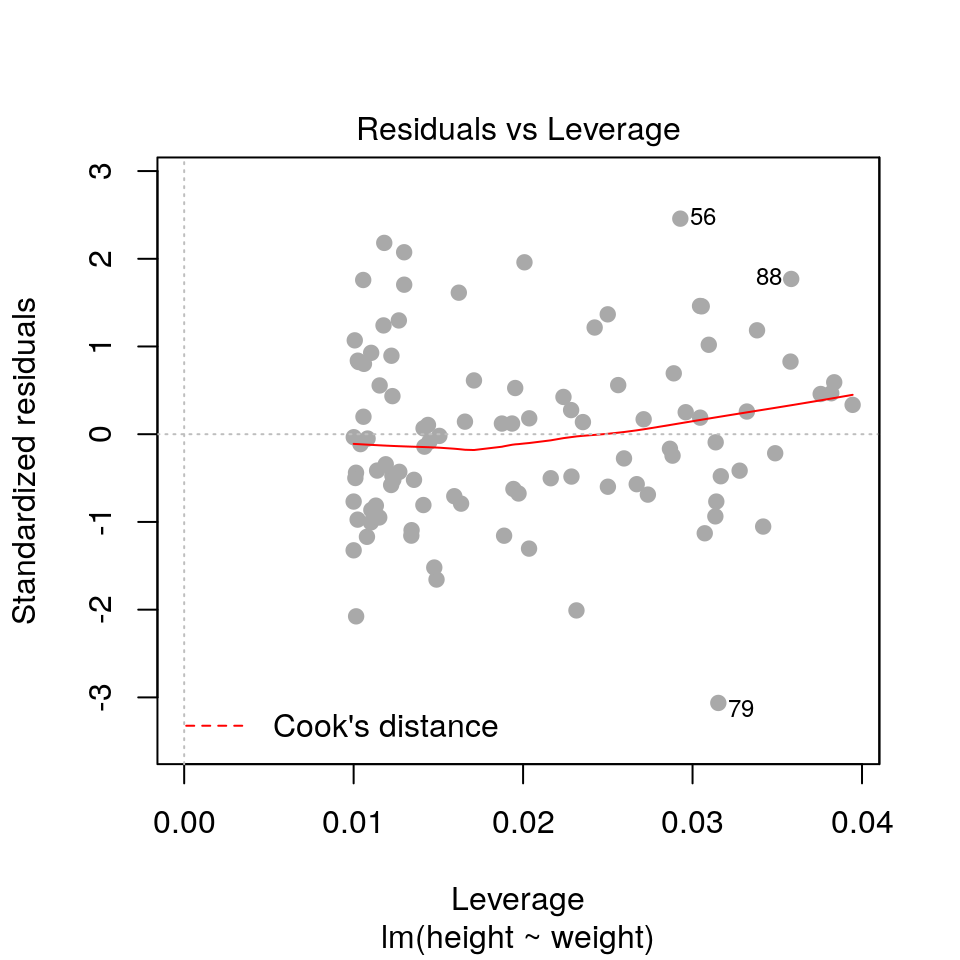
\includegraphics{_main_files/figure-latex/unnamed-chunk-25-1} \end{center}

\begin{itemize}
\tightlist
\item
  \textbf{Leverage}: a measure of how isolated individual points are in
  relation to other points
\item
  \textbf{Cook's Distance}: a measure of how influential a point is to
  the regression
\end{itemize}

These measures help us identify potential outliers.

\newpage

\subsection{QQ plots}\label{qq-plots}

\begin{Shaded}
\begin{Highlighting}[]
\KeywordTok{plot}\NormalTok{(fit, }\DataTypeTok{pch=}\DecValTok{19}\NormalTok{, }\DataTypeTok{col=}\StringTok{'darkgrey'}\NormalTok{, }\DataTypeTok{which=}\DecValTok{2}\NormalTok{)}
\end{Highlighting}
\end{Shaded}

\begin{center}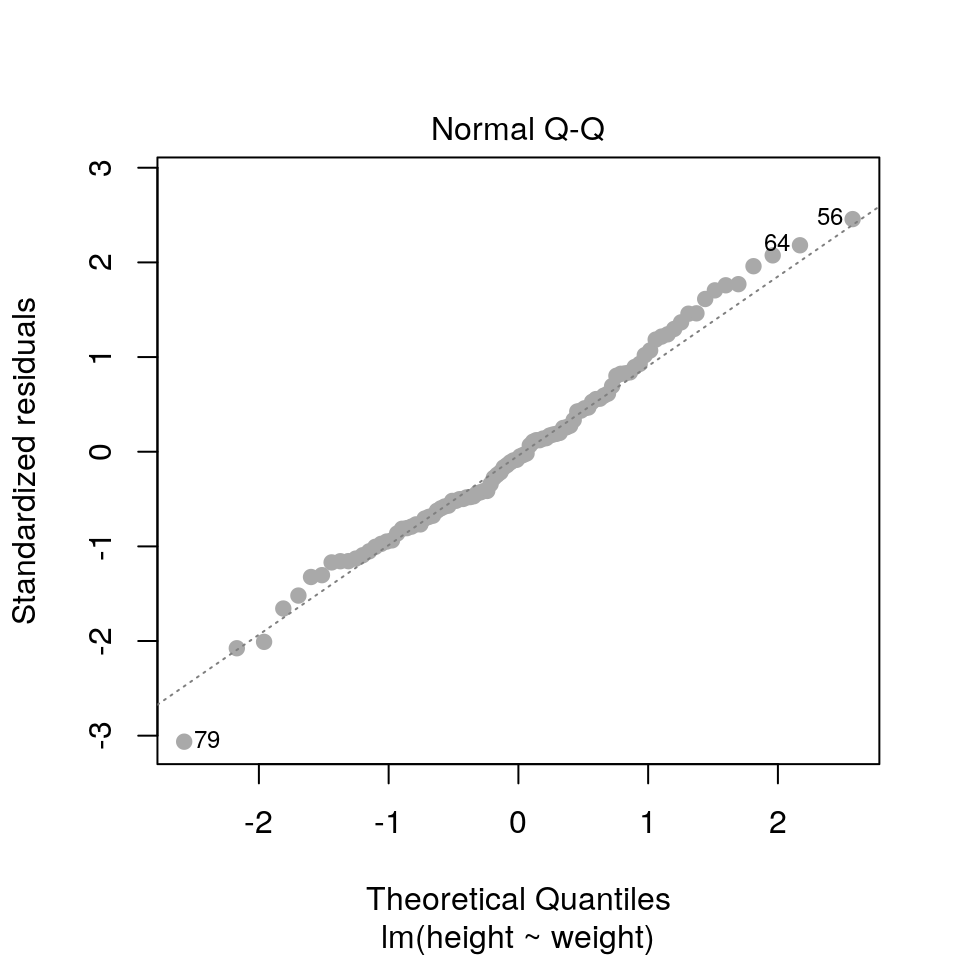
\includegraphics{_main_files/figure-latex/unnamed-chunk-26-1} \end{center}

Here we are checking that the assumption of normally distributed errors
is reasonable. Points should follow the dashed line.

\hypertarget{sec:practical1}{\section{Practical
1}\label{sec:practical1}}

We will use the fruitfly dataset
(\href{https://www.nature.com/articles/294580a0}{Partridge and Farquhar
(1981)}) introduced in the ``Advanced Visualisation and Data Wrangling
in R'', which is summarised again here (do not worry about the details
of the study for now, this is only included for the sake of
completeness):

A cost of increased reproduction in terms of reduced longevity has been
shown for female fruitflies, but not for males. We have data from an
experiment that used a factorial design to assess whether increased
sexual activity affected the lifespan of male fruitflies.

The flies used were an outbred stock. Sexual activity was manipulated by
supplying individual males with one or eight receptive virgin females
per day. The longevity of these males was compared with that of two
control types. The first control consisted of two sets of individual
males kept with one or eight newly inseminated females. Newly
inseminated females will not usually remate for at least two days, and
thus served as a control for any effect of competition with the male for
food or space. The second control was a set of individual males kept
with no females. There were 25 males in each of the five groups, which
were treated identically in number of anaesthetisations (using
\(\mathrm{CO}_2\)) and provision of fresh food medium.

Download the data file from
\href{https://exeter-data-analytics.github.io/StatModelling/_data/fruitfly.rds}{here}
and save it to your working directory.

Since we are working with \texttt{data.frame()} objects, where
appropriate, we have provided examples using both base R or
\texttt{tidyverse} (for those of you who attended the
\href{https://exeter-data-analytics.github.io/AdVis/}{Advanced
Visualisation and Data Wrangling} workshop).

\begin{Shaded}
\begin{Highlighting}[]
\NormalTok{ff <-}\StringTok{ }\KeywordTok{readRDS}\NormalTok{(}\StringTok{"fruitfly.rds"}\NormalTok{)}
\end{Highlighting}
\end{Shaded}

\begin{Shaded}
\begin{Highlighting}[]
\KeywordTok{head}\NormalTok{(ff)}
\end{Highlighting}
\end{Shaded}

\begin{verbatim}
##   partners        type longevity thorax sleep
## 1        8 Inseminated        35   0.64    22
## 2        8 Inseminated        37   0.68     9
## 3        8 Inseminated        49   0.68    49
## 4        8 Inseminated        46   0.72     1
## 5        8 Inseminated        63   0.72    23
## 6        8 Inseminated        39   0.76    83
\end{verbatim}

For the purpose of this practical we will assume that the no female case
is the control case, whilst the inseminated and virgin female cases are
the treatment cases.

\begin{itemize}
\tightlist
\item
  \textbf{partners}: number of companions (0, 1 or 8)
\item
  \textbf{type}: type of companion (inseminated female; virgin female;
  control (when partners = 0))
\item
  \textbf{longevity}: lifespan, in days
\item
  \textbf{thorax}: length of thorax, in mm
\item
  \textbf{sleep}: percentage of each day spent sleeping
\end{itemize}

\hypertarget{tsk1}{}\bblockT[Task]{\phantomsection\label{sol1}1}

Produce a scatterplot of \texttt{longevity} against \texttt{thorax}.
What does the relationship look like? \eblockT

\hyperlink{sol1}{\buttonS{Show Solution on P\colpageref{tsk1}}}

\hypertarget{tsk2}{}\bblockT[Task]{\phantomsection\label{sol2}2}

\begin{enumerate}
\def\labelenumi{\arabic{enumi}.}
\tightlist
\item
  Fit a linear model with lifespan as response variable and thorax
  length as explanatory variable.
\item
  Display a summary of the fit, together with the 97\% confidence
  interval for the estimated parameters.
\item
  Show the diagnostic plots for the model.
\end{enumerate}

\eblockT

\hyperlink{sol2}{\buttonS{Show Solution on P\colpageref{tsk2}}}

\hypertarget{sec:prediction}{\section{Prediction}\label{sec:prediction}}

One of the key benefits of fitting a statistical model is that we can
use it to produce predictions of the response variable for new values of
the explanatory variable(s). We can do this using the \texttt{predict()}
function in R. For example, in the fruitflies example above, we may want
to produce estimates of average \texttt{longevity} for given values of
\texttt{thorax}. To do this we must create a new \texttt{data.frame}
object containing all the values of \textbf{explanatory} variables that
we want to use for our prediction.

\begin{quote}
\textbf{Note}: we only require the \textbf{\emph{explanatory}} variables
in this new data frame, the \textbf{\emph{response}} variable will be
generated from the model.
\end{quote}

For example, if we wanted to produce an estimate of \texttt{longevity}
for an average individual with a \texttt{thorax} length of 0.8mm, we can
run:

\begin{Shaded}
\begin{Highlighting}[]
\NormalTok{## produce predicted longevity for thorax = 0.8mm}
\NormalTok{newdata <-}\StringTok{ }\KeywordTok{data.frame}\NormalTok{(}\DataTypeTok{thorax =} \FloatTok{0.8}\NormalTok{)}
\KeywordTok{predict}\NormalTok{(fit, newdata)}
\end{Highlighting}
\end{Shaded}

\begin{verbatim}
##        1 
## 54.41478
\end{verbatim}

We can also use this to produce \textbf{confidence} or
\textbf{prediction} intervals as follows:

\begin{Shaded}
\begin{Highlighting}[]
\NormalTok{## produce predicted longevity for thorax = 0.8mm}
\NormalTok{newdata <-}\StringTok{ }\KeywordTok{data.frame}\NormalTok{(}\DataTypeTok{thorax =} \FloatTok{0.8}\NormalTok{)}
\KeywordTok{predict}\NormalTok{(fit, newdata, }\DataTypeTok{interval =} \StringTok{"confidence"}\NormalTok{, }\DataTypeTok{level =} \FloatTok{0.97}\NormalTok{)}
\end{Highlighting}
\end{Shaded}

\begin{verbatim}
##        fit      lwr      upr
## 1 54.41478 51.64686 57.18269
\end{verbatim}

\begin{quote}
\textbf{Note}: If you predict \emph{without} an \texttt{interval}
argument, the \texttt{predict()} function returns a \texttt{vector},
otherwise it returns a \texttt{matrix}.
\end{quote}

\textbf{Aside}: there are two types of intervals that you might want to
produce: \textbf{confidence} or \textbf{prediction} intervals.

\begin{itemize}
\tightlist
\item
  \textbf{Confidence} intervals: these correspond to the uncertainty
  surrounding our estimate of an \textbf{average} individual (i.e.~it
  represents the uncertainty in the \textbf{mean}:
  \(y = \beta_0 + \beta_1 x\)
\item
  \textbf{Prediction} intervals: these correspond to the uncertainty
  surrounding an \textbf{individual} observation:
  \(y_i = \beta_0 + \beta_1 x_i + \epsilon_i\).
\end{itemize}

If the model fits well, then we would expect \(100(1 - \alpha)\)\% of
the individual measurements to lie within the \textbf{prediction}
interval, where \(\alpha\) is the significance level (so
\(\alpha = 0.03\) corresponds to a 97\% confidence interval).

\newpage

The \texttt{predict()} function can be used as a very general way to
produce plots of the fitted values over the observed data. For example,
let's consider that we wish to add our fitted regression line to our
observed data plot.

\begin{Shaded}
\begin{Highlighting}[]
\KeywordTok{plot}\NormalTok{(longevity }\OperatorTok{~}\StringTok{ }\NormalTok{thorax, }\DataTypeTok{data =}\NormalTok{ ff, }\DataTypeTok{pch =} \DecValTok{19}\NormalTok{, }\DataTypeTok{col=}\StringTok{'darkgrey'}\NormalTok{)}
\end{Highlighting}
\end{Shaded}

\begin{center}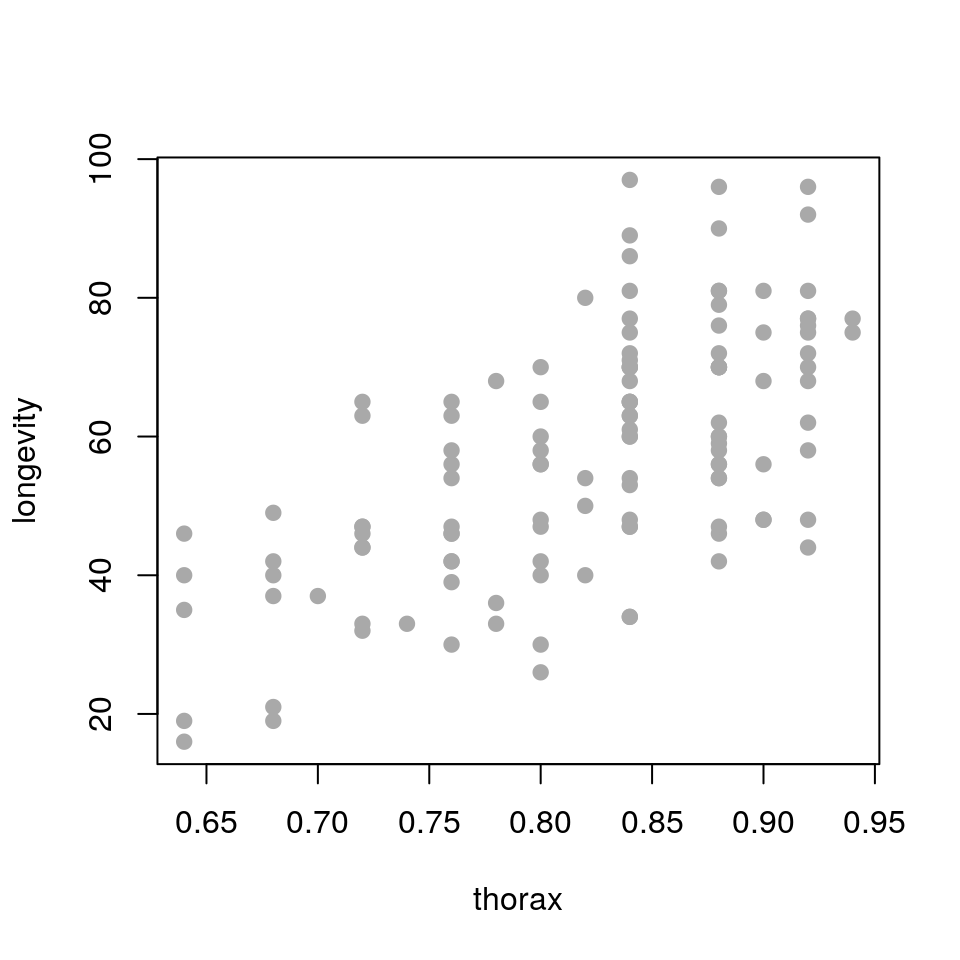
\includegraphics{_main_files/figure-latex/unnamed-chunk-36-1} \end{center}

There are various ways to add the correct regression line to this plot,
but we will show you a general way that can be used for lots of
different types of models. Firstly, we generate a range of
\(x\)-coordinates that we wish to predict to e.g.

\begin{Shaded}
\begin{Highlighting}[]
\NormalTok{## create new data frame to predict to}
\NormalTok{newdata <-}\StringTok{ }\KeywordTok{data.frame}\NormalTok{(}\DataTypeTok{thorax=}\KeywordTok{seq}\NormalTok{(}\KeywordTok{min}\NormalTok{(ff}\OperatorTok{$}\NormalTok{thorax), }\KeywordTok{max}\NormalTok{(ff}\OperatorTok{$}\NormalTok{thorax), }\DataTypeTok{length.out=}\DecValTok{50}\NormalTok{))}
\end{Highlighting}
\end{Shaded}

We then have to use the model to predict the mean \texttt{longevity} at
each of these \texttt{thorax} values:

\begin{Shaded}
\begin{Highlighting}[]
\NormalTok{## predict longevity form the model}
\NormalTok{newdata <-}\StringTok{ }\KeywordTok{cbind}\NormalTok{(newdata, }\DataTypeTok{longevity=}\KeywordTok{predict}\NormalTok{(fit, newdata))}
\end{Highlighting}
\end{Shaded}

Just as an illustration we will overlay these predictions onto the
original scatterplot as points:

\begin{Shaded}
\begin{Highlighting}[]
\NormalTok{## add predicted points to original plot}
\KeywordTok{plot}\NormalTok{(longevity }\OperatorTok{~}\StringTok{ }\NormalTok{thorax, }\DataTypeTok{data =}\NormalTok{ ff, }\DataTypeTok{pch =} \DecValTok{19}\NormalTok{, }\DataTypeTok{col=}\StringTok{'darkgrey'}\NormalTok{)}
\KeywordTok{points}\NormalTok{(longevity }\OperatorTok{~}\StringTok{ }\NormalTok{thorax, }\DataTypeTok{data =}\NormalTok{ newdata, }\DataTypeTok{pch =} \DecValTok{19}\NormalTok{, }\DataTypeTok{col =} \StringTok{"red"}\NormalTok{)}
\end{Highlighting}
\end{Shaded}

\begin{center}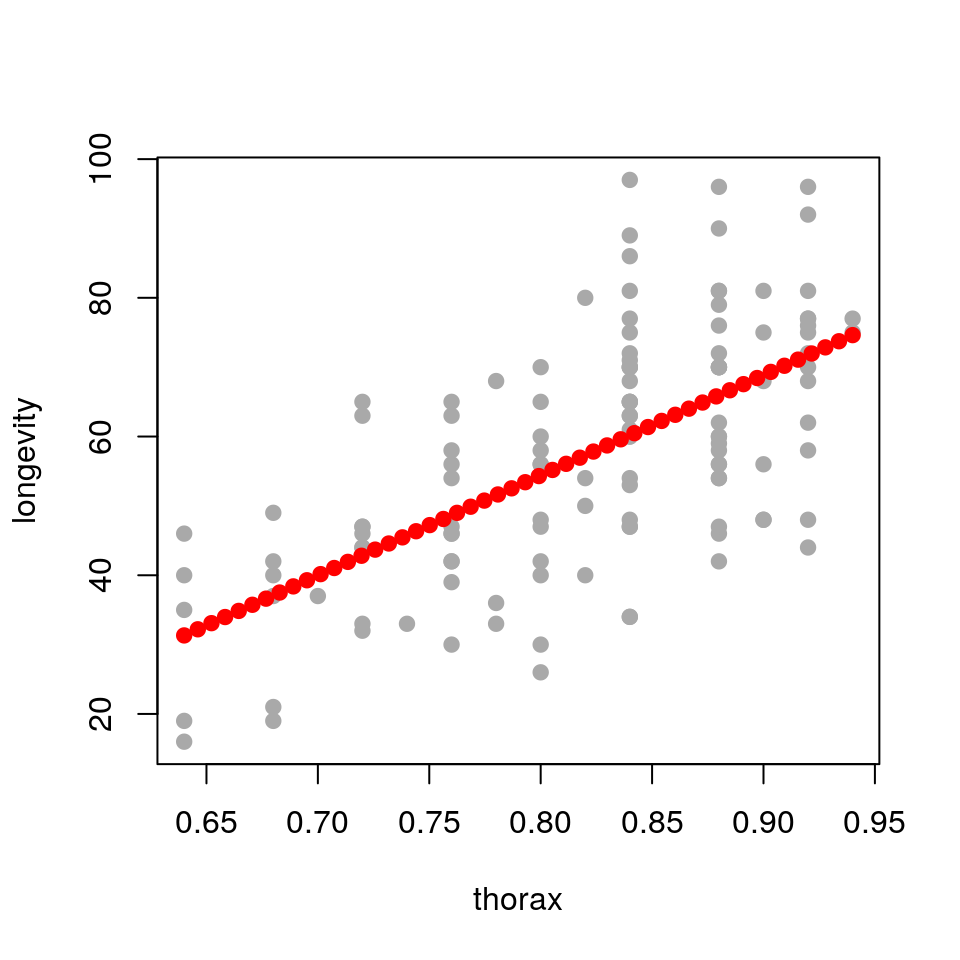
\includegraphics{_main_files/figure-latex/unnamed-chunk-39-1} \end{center}

So we have used the \texttt{predict()} function to produce predicted
coordinates that we can overlay on the original scatterplot. In practice
we would usually plot these predictions as a \textbf{line} rather than
points. This approach is particularly useful if the predictions that we
wish to plot are not straight lines (such as when we generate
\textbf{confidence} or \textbf{prediction} intervals). To complete this
example we will now plot the fitted line and associated confidence
interval as follows:

\begin{Shaded}
\begin{Highlighting}[]
\NormalTok{## create new data frame to predict to}
\NormalTok{newdata <-}\StringTok{ }\KeywordTok{data.frame}\NormalTok{(}\DataTypeTok{thorax=}\KeywordTok{seq}\NormalTok{(}\KeywordTok{min}\NormalTok{(ff}\OperatorTok{$}\NormalTok{thorax), }\KeywordTok{max}\NormalTok{(ff}\OperatorTok{$}\NormalTok{thorax), }\DataTypeTok{length.out=}\DecValTok{50}\NormalTok{))}

\NormalTok{## produce predictions and intervals}
\NormalTok{newdata <-}\StringTok{ }\KeywordTok{cbind}\NormalTok{(newdata, }\KeywordTok{predict}\NormalTok{(fit, newdata, }\DataTypeTok{interval=}\StringTok{"confidence"}\NormalTok{, }\DataTypeTok{level=}\FloatTok{0.97}\NormalTok{))}
\NormalTok{newdata}\OperatorTok{$}\NormalTok{longevity <-}\StringTok{ }\NormalTok{newdata}\OperatorTok{$}\NormalTok{fit}
\NormalTok{newdata}\OperatorTok{$}\NormalTok{fit <-}\StringTok{ }\OtherTok{NULL}
\end{Highlighting}
\end{Shaded}

\newpage

\bmp
\bblockST{Base R}

\begin{Shaded}
\begin{Highlighting}[]
\NormalTok{## plot fitted line against the raw data}
\KeywordTok{plot}\NormalTok{(longevity }\OperatorTok{~}\StringTok{ }\NormalTok{thorax, }\DataTypeTok{data =}\NormalTok{ ff, }
     \DataTypeTok{pch =} \DecValTok{19}\NormalTok{, }\DataTypeTok{col=}\StringTok{'darkgrey'}\NormalTok{,}
     \DataTypeTok{main =} \StringTok{"Fitted regression line}
\StringTok{     with 97% confidence interval"}\NormalTok{)}
\KeywordTok{lines}\NormalTok{(longevity }\OperatorTok{~}\StringTok{ }\NormalTok{thorax, }\DataTypeTok{data =}\NormalTok{ newdata)}
\KeywordTok{lines}\NormalTok{(lwr }\OperatorTok{~}\StringTok{ }\NormalTok{thorax, }\DataTypeTok{data =}\NormalTok{ newdata, }\DataTypeTok{lty =} \DecValTok{2}\NormalTok{)}
\KeywordTok{lines}\NormalTok{(upr }\OperatorTok{~}\StringTok{ }\NormalTok{thorax, }\DataTypeTok{data =}\NormalTok{ newdata, }\DataTypeTok{lty =} \DecValTok{2}\NormalTok{)}
\end{Highlighting}
\end{Shaded}

\begin{center}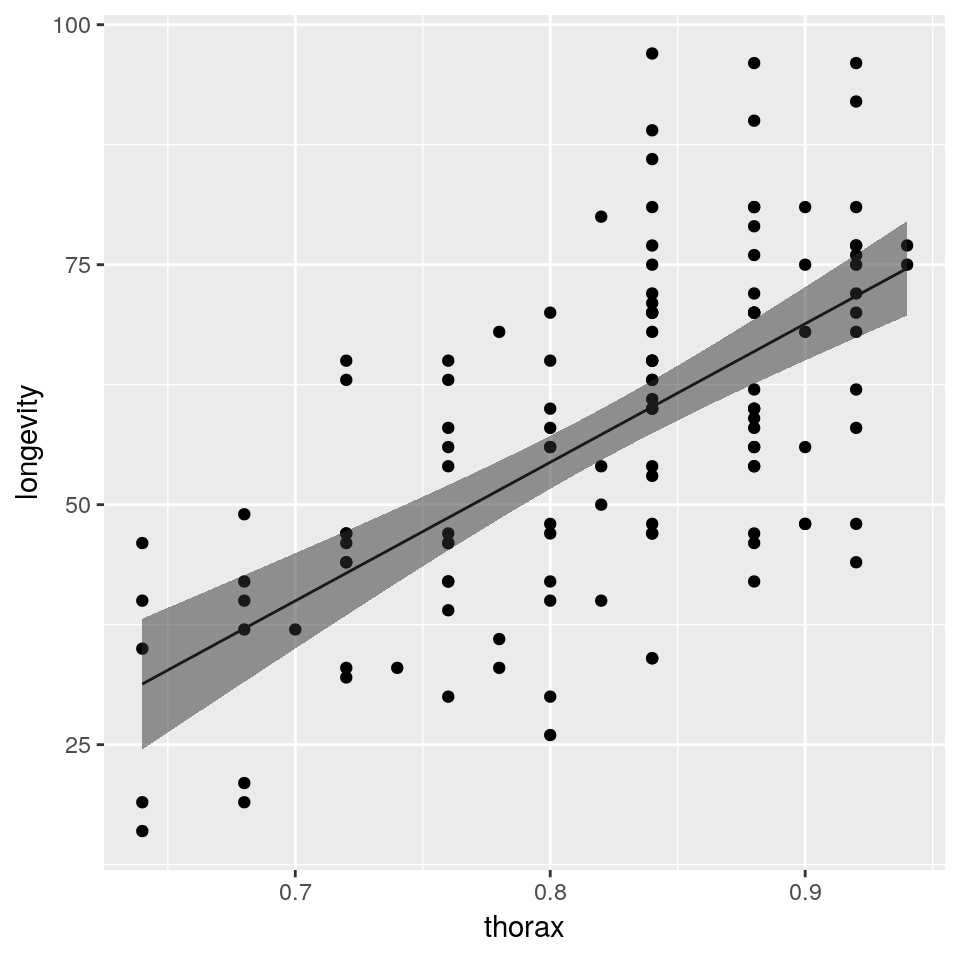
\includegraphics{_main_files/figure-latex/unnamed-chunk-193-1} \end{center}

\eblockST
\emp
\hspace{0.01\textwidth} \bmp\bblockST{\texttt{tidyverse}}

\begin{Shaded}
\begin{Highlighting}[]
\NormalTok{## plot fitted line against the raw data}
\KeywordTok{ggplot}\NormalTok{(}\DataTypeTok{mapping =} 
        \KeywordTok{aes}\NormalTok{(}\DataTypeTok{x =}\NormalTok{ thorax, }\DataTypeTok{y =}\NormalTok{ longevity)) }\OperatorTok{+}
\StringTok{    }\KeywordTok{geom_point}\NormalTok{(}\DataTypeTok{data =}\NormalTok{ ff) }\OperatorTok{+}
\StringTok{    }\KeywordTok{geom_line}\NormalTok{(}\DataTypeTok{data =}\NormalTok{ newdata) }\OperatorTok{+}
\StringTok{    }\KeywordTok{geom_ribbon}\NormalTok{(}
        \KeywordTok{aes}\NormalTok{(}\DataTypeTok{ymin =}\NormalTok{ lwr, }\DataTypeTok{ymax =}\NormalTok{ upr), }
        \DataTypeTok{data =}\NormalTok{ newdata, }\DataTypeTok{alpha =} \FloatTok{0.5}\NormalTok{)}
\end{Highlighting}
\end{Shaded}

\begin{center}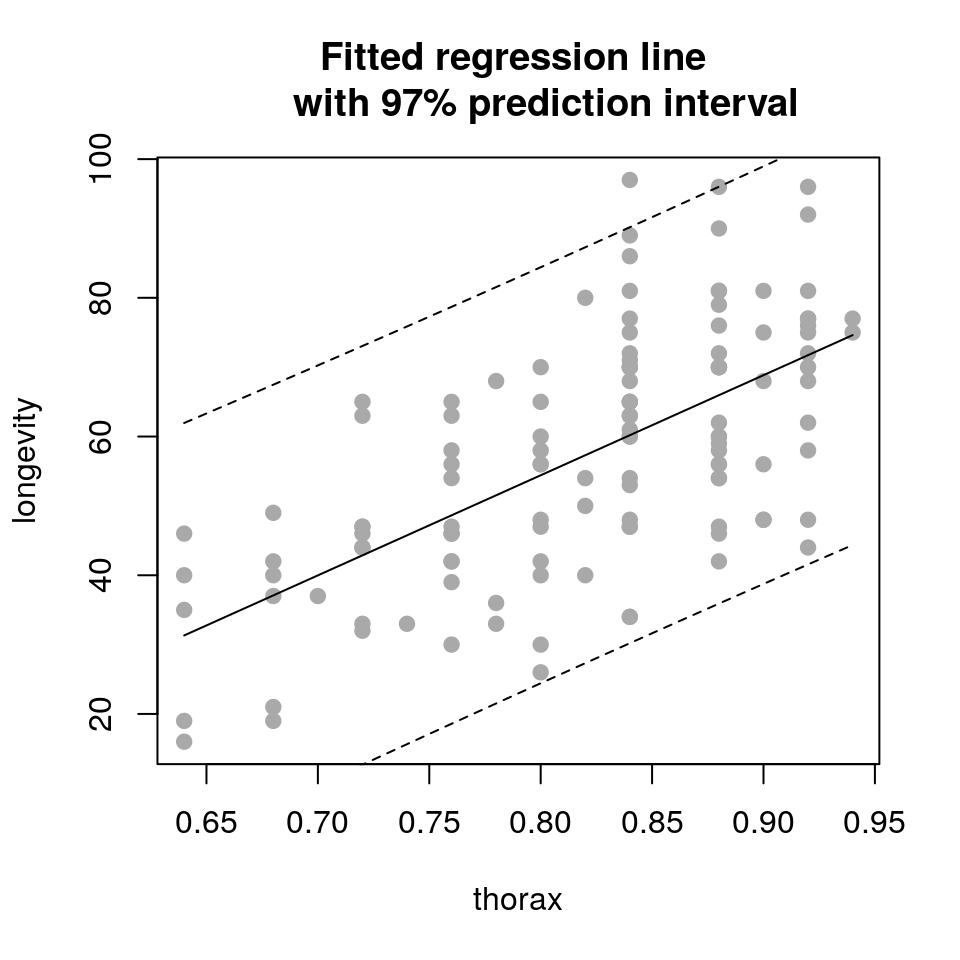
\includegraphics{_main_files/figure-latex/unnamed-chunk-194-1} \end{center}

\eblockST
\emp

\hypertarget{tsk3}{}\bblockT[Task]{\phantomsection\label{sol3}3}

Produce the same plot but with a 97\% \textbf{prediction} interval
\eblockT

\hyperlink{sol3}{\buttonS{Show Solution on P\colpageref{tsk3}}}

\section{Multiple linear regression}\label{multiple-linear-regression}

So far we have looked at examples with one response and one explanatory
variable. In most applications we will have several variables that
affect our outcome. Extending our simple linear regression model to
accommodate multiple explanatory variables is straightforward, we just
add them to the model.

Using our illustrative example of height vs weight, let's add another
explanatory variable, for example, the mean height of the individual's
parents (\texttt{heightParents}). Our linear model is defined as
follows:

\[
\begin{aligned}
y_i & = \beta_0 + \beta_1x_{1i} + \beta_2x_{2i} + \epsilon_i \\
\epsilon_i & \sim \mathcal{N}(0, \sigma^2)
\end{aligned}
\] Or in English:

\[
\begin{aligned}
\mathrm{height}_i & = \beta_0 + \beta_1\mathrm{weight}_i + + \beta_2\mathrm{heightParents}_i+ \epsilon_i \\
\epsilon_i & \sim \mathcal{N}(0, \sigma^2)
\end{aligned}
\]

Let us make up some data again and plot it.

\begin{Shaded}
\begin{Highlighting}[]
\KeywordTok{set.seed}\NormalTok{(}\DecValTok{451}\NormalTok{)}

\NormalTok{## no. of observations}
\NormalTok{N <-}\StringTok{ }\DecValTok{100} 

\NormalTok{## hypothetical weights in kg}
\NormalTok{weight <-}\StringTok{ }\KeywordTok{runif}\NormalTok{(}\DataTypeTok{n=}\NormalTok{N, }\DataTypeTok{min=}\DecValTok{60}\NormalTok{, }\DataTypeTok{max=}\DecValTok{100}\NormalTok{) }

\NormalTok{## hypothetical mean heights of parents in cm}
\NormalTok{heightParents <-}\StringTok{ }\KeywordTok{runif}\NormalTok{(}\DataTypeTok{n=}\NormalTok{N, }\DataTypeTok{min=}\DecValTok{130}\NormalTok{, }\DataTypeTok{max=}\DecValTok{210}\NormalTok{) }

\NormalTok{## hypothetical heights in cm}
\NormalTok{height <-}\StringTok{ }\FloatTok{0.1}\OperatorTok{*}\NormalTok{weight }\OperatorTok{+}\StringTok{ }\FloatTok{1.05}\OperatorTok{*}\NormalTok{heightParents }\OperatorTok{+}\StringTok{ }\KeywordTok{rnorm}\NormalTok{(}\DataTypeTok{n=}\NormalTok{N, }\DataTypeTok{mean=}\DecValTok{0}\NormalTok{, }\DataTypeTok{sd=}\DecValTok{10}\NormalTok{) }

\NormalTok{## store as df}
\NormalTok{df <-}\StringTok{ }\KeywordTok{data.frame}\NormalTok{(}\DataTypeTok{weight=}\NormalTok{weight, }\DataTypeTok{heightParents=}\NormalTok{heightParents, }\DataTypeTok{height=}\NormalTok{height) }

\NormalTok{## Plot}
\KeywordTok{library}\NormalTok{(scatterplot3d) ## library needed for 3D plotting}
\KeywordTok{scatterplot3d}\NormalTok{(weight, heightParents, height, }\DataTypeTok{pch=}\DecValTok{19}\NormalTok{, }\DataTypeTok{xlab=}\StringTok{'Weight (kg)'}\NormalTok{, }
              \DataTypeTok{ylab=}\StringTok{'Height of Parents (cm)'}\NormalTok{, }\DataTypeTok{zlab=}\StringTok{'Height (cm)'}\NormalTok{, }\DataTypeTok{color=}\StringTok{'grey'}\NormalTok{)}
\end{Highlighting}
\end{Shaded}

\begin{center}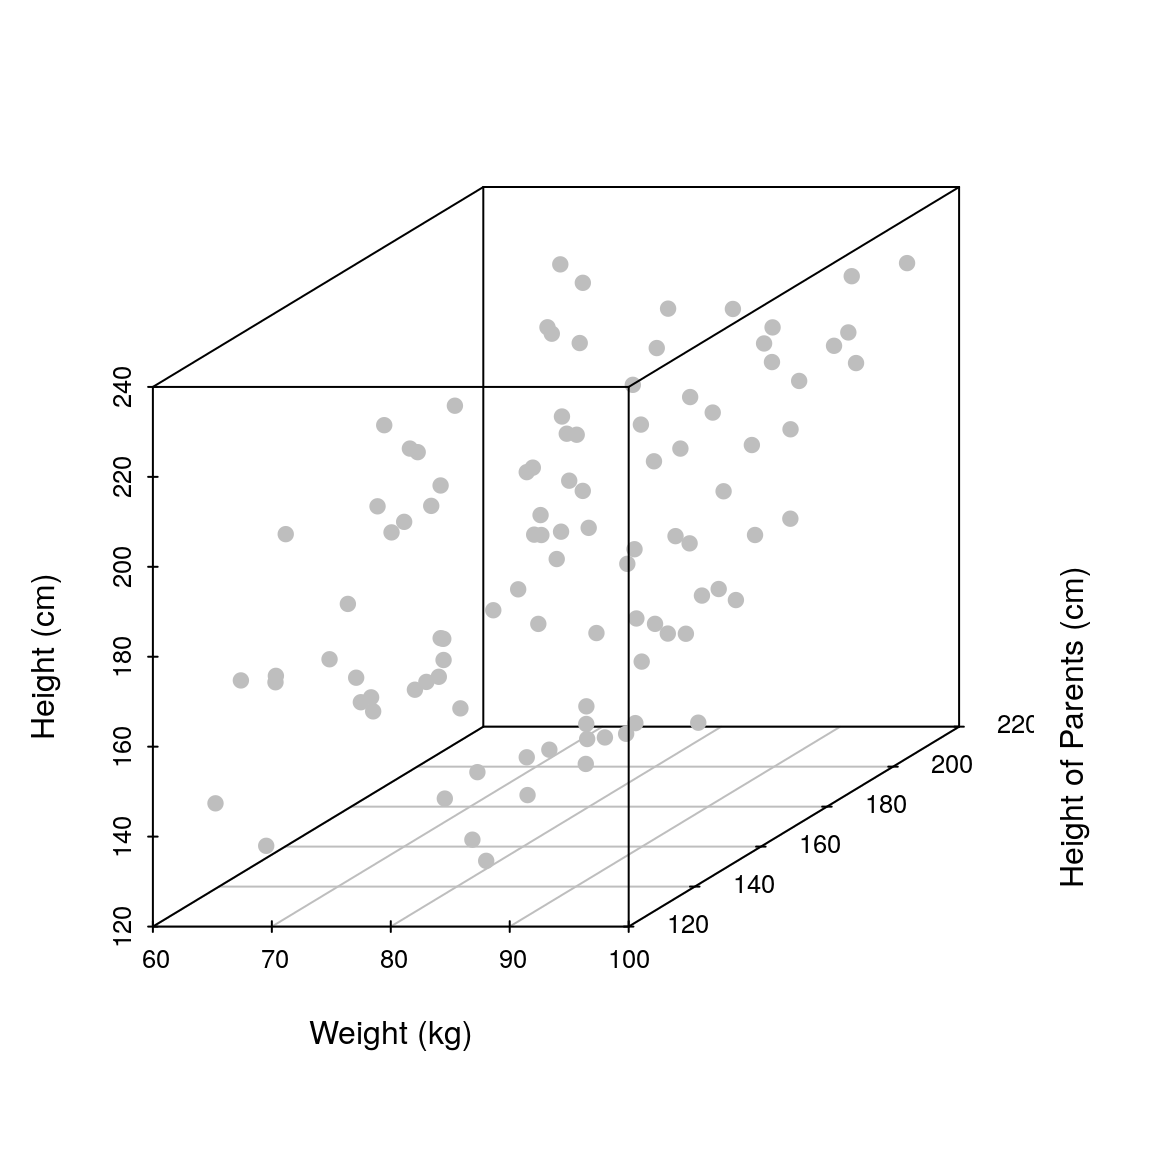
\includegraphics[width=0.6\linewidth]{_main_files/figure-latex/unnamed-chunk-44-1} \end{center}

Note how by adding another explanatory variable we are \emph{spreading}
the observations across an additional dimension. That is, we go from a
2D plot to a 3D plot (if we add a third explanatory variable we would
need a 4D plot). It is important to keep this in mind; the more
explanatory variables we add the more we spread our data thinly across
multiple dimensions. In practice, this means that our observations will
be sparsely scattered across a high dimensional space, making it hard to
fit a robust linear model. In the limit, when we have more explanatory
variables than observations, we would not be able to fit a linear model
at all (unless we employ a different statistical framework and impose
further assumptions/constraints).

The objective of linear modelling is still the same, finding the
``best'' straight line, or in this case a \textbf{hyperplane} (a line in
higher dimensions). You can think of a \textbf{hyperplane} as a (rigid)
sheet of paper, where the objective is to place it such that it passes
as close as possible to the observed data.

To fit a multiple linear regression model we use the
\href{https://www.rdocumentation.org/packages/stats/versions/3.5.1/topics/lm}{\texttt{lm()}}
function again and pass the appropriate \textbf{formula} object which
has the form of
\texttt{response\ \textasciitilde{}\ explanatory\_1\ +\ explanatory\_2}.
In in our case this will be
\texttt{height\ \textasciitilde{}\ weight\ +\ heightParents}.

\begin{Shaded}
\begin{Highlighting}[]
\NormalTok{fit <-}\StringTok{ }\KeywordTok{lm}\NormalTok{(height }\OperatorTok{~}\StringTok{ }\NormalTok{weight }\OperatorTok{+}\StringTok{ }\NormalTok{heightParents, df)}
\end{Highlighting}
\end{Shaded}

Let us plot the resultant model first (i.e the hyperplane).

\begin{Shaded}
\begin{Highlighting}[]
\NormalTok{hFig <-}\StringTok{ }\KeywordTok{scatterplot3d}\NormalTok{(weight, heightParents, height, }\DataTypeTok{pch=}\DecValTok{19}\NormalTok{, }\DataTypeTok{xlab=}\StringTok{'Weight (kg)'}\NormalTok{, }
                      \DataTypeTok{ylab=}\StringTok{'Height of Parents (cm)'}\NormalTok{, }\DataTypeTok{zlab=}\StringTok{'Height (cm)'}\NormalTok{, }\DataTypeTok{color=}\StringTok{'grey'}\NormalTok{)}
\NormalTok{hFig}\OperatorTok{$}\KeywordTok{plane3d}\NormalTok{(fit, }\DataTypeTok{draw_polygon=}\OtherTok{TRUE}\NormalTok{)}
\end{Highlighting}
\end{Shaded}

\begin{center}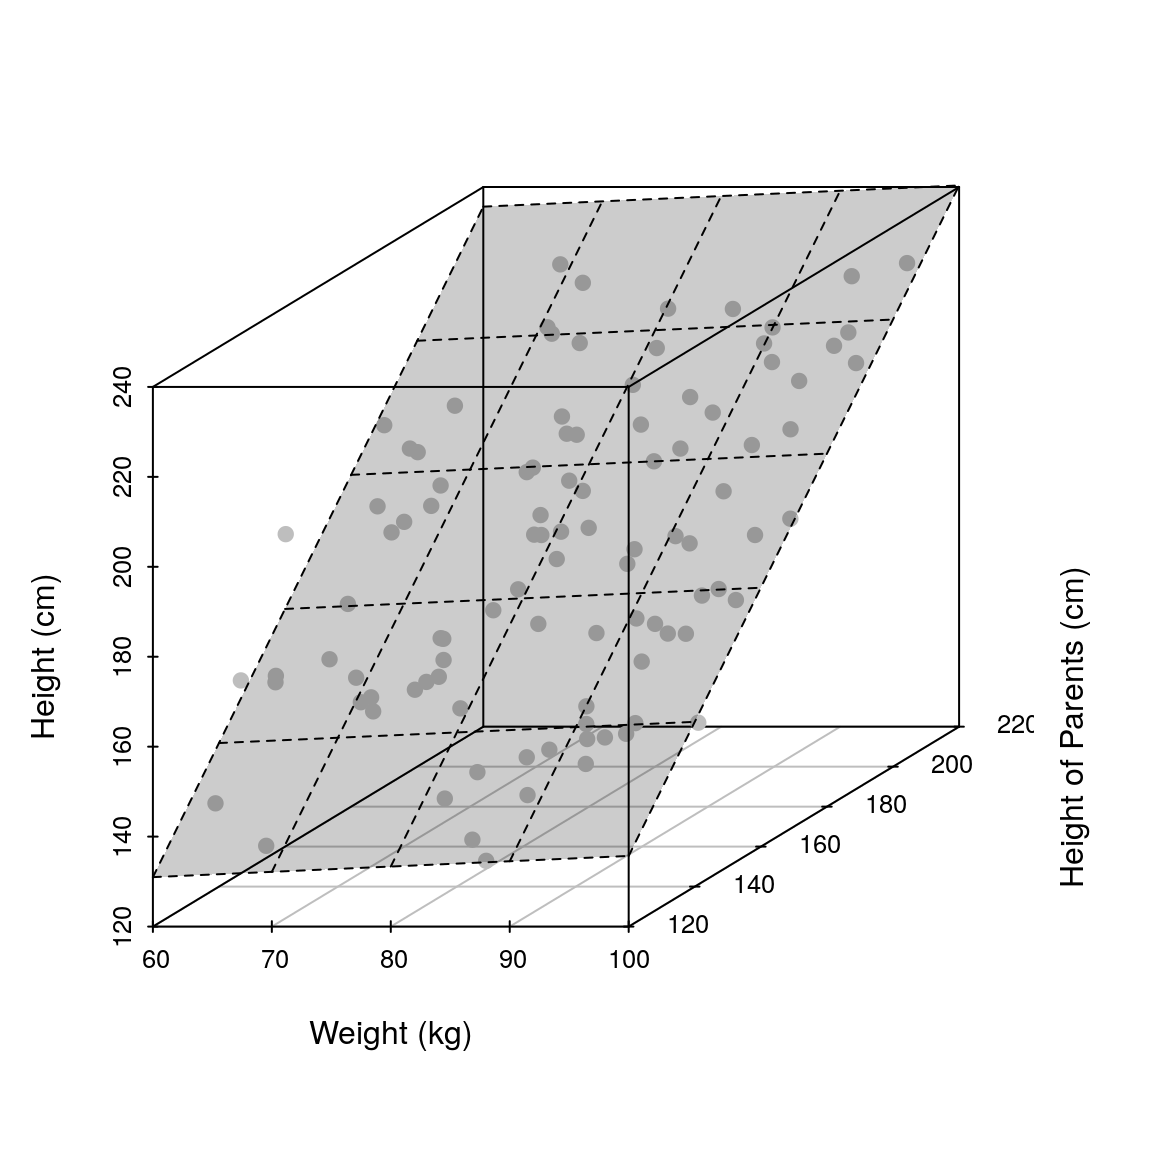
\includegraphics[width=0.6\linewidth]{_main_files/figure-latex/unnamed-chunk-46-1} \end{center}

\newpage

Let us look at the fit's summary

\begin{Shaded}
\begin{Highlighting}[]
\KeywordTok{summary}\NormalTok{(fit)}
\end{Highlighting}
\end{Shaded}

\begin{verbatim}
## 
## Call:
## lm(formula = height ~ weight + heightParents, data = df)
## 
## Residuals:
##     Min      1Q  Median      3Q     Max 
## -28.578  -6.052   0.235   6.027  27.829 
## 
## Coefficients:
##               Estimate Std. Error t value Pr(>|t|)    
## (Intercept)   -1.65589   10.70833  -0.155    0.877    
## weight         0.11790    0.09198   1.282    0.203    
## heightParents  1.04644    0.04707  22.233   <2e-16 ***
## ---
## Signif. codes:  0 '***' 0.001 '**' 0.01 '*' 0.05 '.' 0.1 ' ' 1
## 
## Residual standard error: 10.19 on 97 degrees of freedom
## Multiple R-squared:  0.8372, Adjusted R-squared:  0.8338 
## F-statistic: 249.4 on 2 and 97 DF,  p-value: < 2.2e-16
\end{verbatim}

Same as before, the \texttt{(Intercept)=} -1.656 cm, \texttt{weight=}
0.1179 cm/kg and \texttt{heightParents=} 1.046 cm/cm are the
\(\beta_0\), \(\beta_1\) and \(\beta_2\) parameters.

\begin{itemize}
\tightlist
\item
  The \(\beta_0\) parameter (intercept) is the expected height of
  someone that weighs 0 kg \emph{and} whose parents have a mean height
  of 0 cm. Again, this parameter is not useful in this case.
\item
  The \(\beta_1\) parameter tells us about the relationship between
  \texttt{height} and \texttt{weight}. For every 1 kg increase in weight
  on \emph{average} the height increases by 0.1179 cm.
\item
  The \(\beta_2\) parameter tells us about the relationship between
  \texttt{height} and \texttt{heightParents}. For every 1 cm increase in
  mean height of parents on \emph{average} the person's height increases
  by 1.046 cm.
\end{itemize}

\newpage

As before we look at the model diagnostic plots to check the model fit.

\begin{Shaded}
\begin{Highlighting}[]
\KeywordTok{par}\NormalTok{(}\DataTypeTok{mfrow=}\KeywordTok{c}\NormalTok{(}\DecValTok{2}\NormalTok{, }\DecValTok{2}\NormalTok{))}
\KeywordTok{plot}\NormalTok{(fit, }\DataTypeTok{pch=}\DecValTok{19}\NormalTok{, }\DataTypeTok{col=}\StringTok{'darkgrey'}\NormalTok{)}
\end{Highlighting}
\end{Shaded}

\begin{center}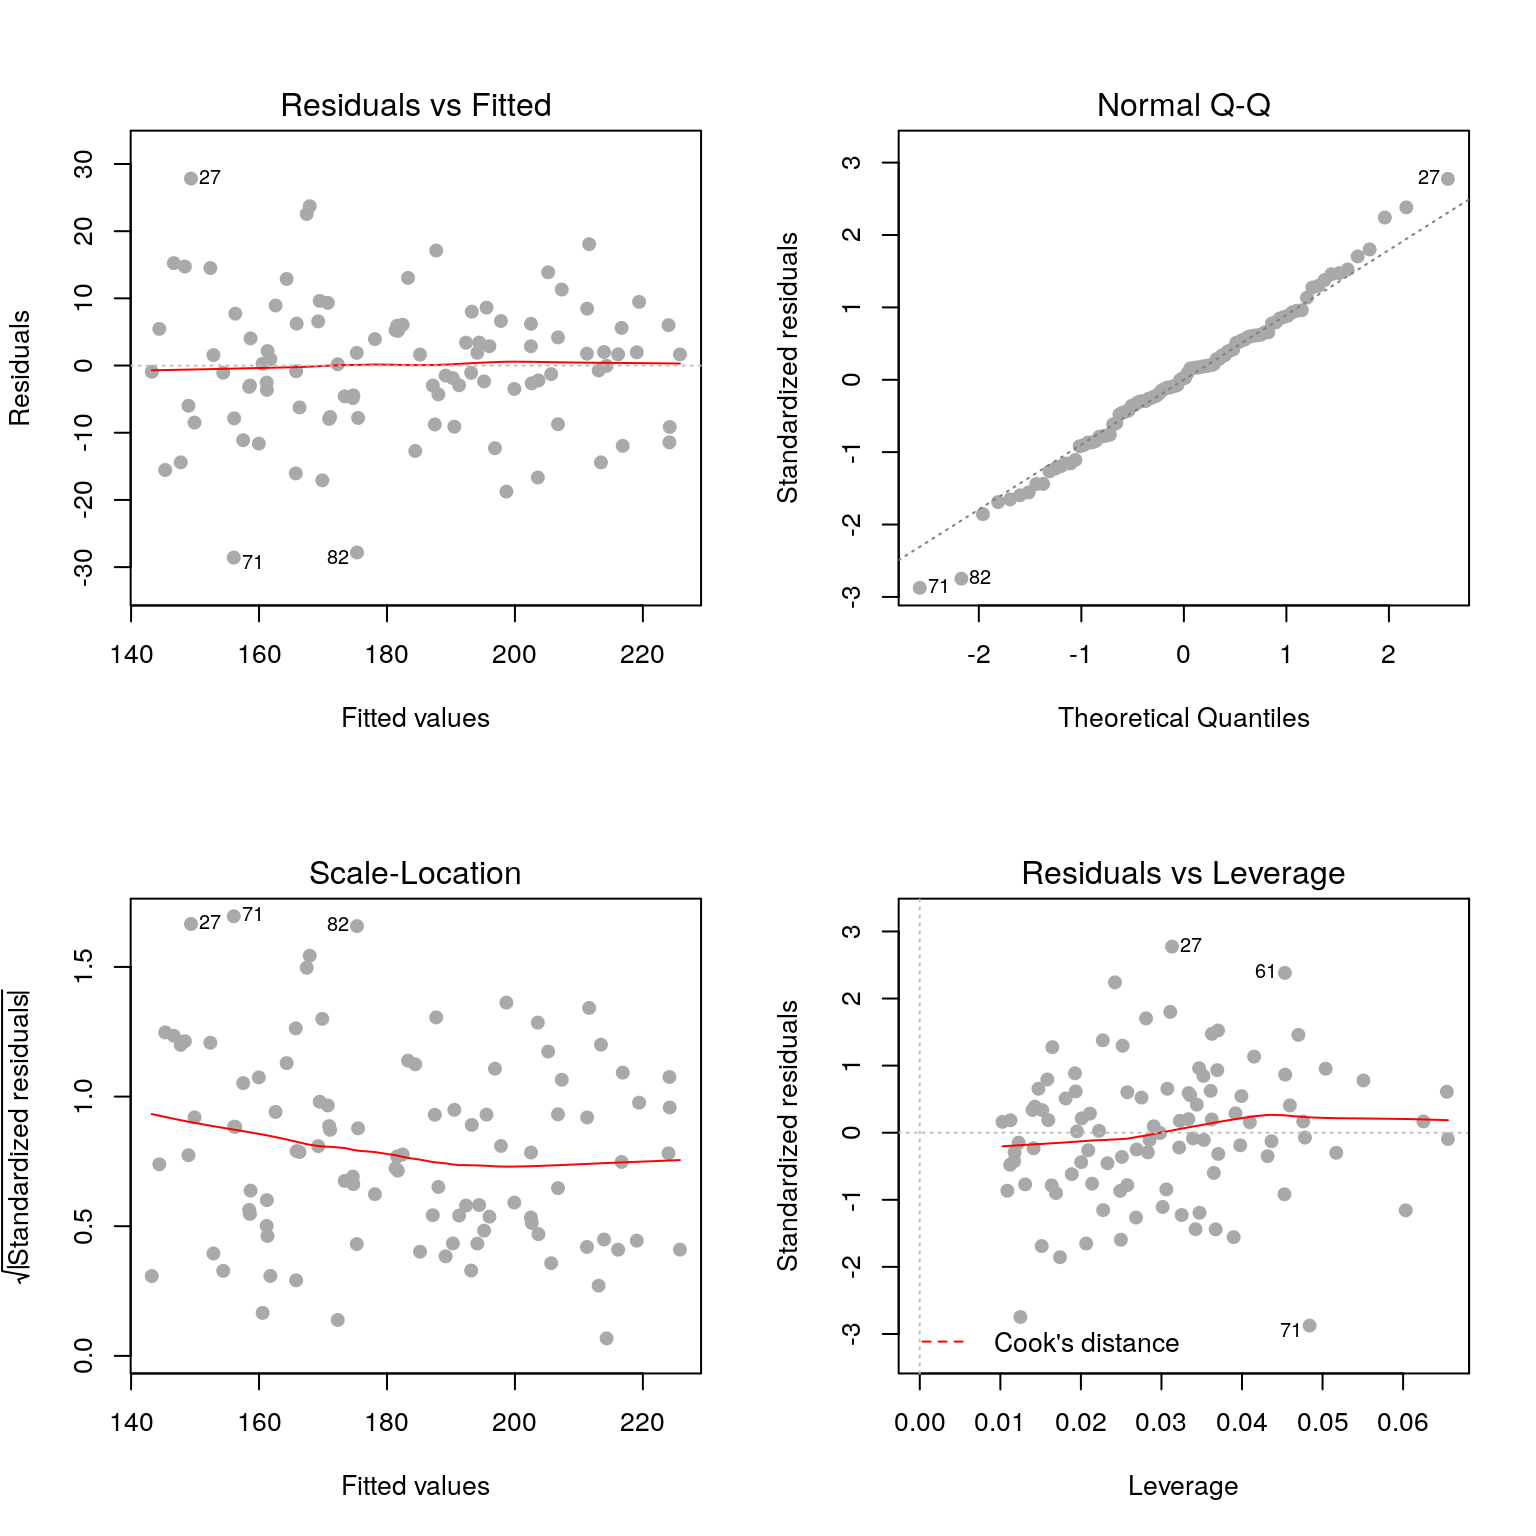
\includegraphics{_main_files/figure-latex/unnamed-chunk-48-1} \end{center}

We can extend this framework to any arbitrary large number of
explanatory variables. The model is:

\[
\begin{aligned}
y_i & = \beta_0 + \beta_1x_{1i} + \ldots + \beta_px_{pi} + \epsilon_i \\
\epsilon_i & \sim \mathcal{N}(0, \sigma^2)
\end{aligned}
\] Where \(i\) is an index that goes from 1 to \(n\) (the total number
of observations) and \(p\) is the total number of explanatory variables.
Hopefully it is now clearer why statisticians use Greek letters
\(\beta_0, \ldots, \beta_p\), else the equation would be too long to
write in English

outcome = intercept + ((gradient outcome vs explanatory variable 1) x
(explanatory variable 1)) + ((gradient outcome vs explanatory variable
2) x (explanatory variable 2)) + \ldots{})

\section{Practical 2}\label{practical-2}

We will use the fruitfly dataset
(\href{https://www.nature.com/articles/294580a0}{Partridge and Farquhar
(1981)}) as we did in the previous practical

\hypertarget{tsk4}{}\bblockT[Task]{\phantomsection\label{sol4}4}

\begin{enumerate}
\def\labelenumi{\arabic{enumi}.}
\tightlist
\item
  Fit a linear model with lifespan as response variable and thorax
  length and sleep as explanatory variables
\item
  Display a summary of the fit, together with the 97\% confidence
  intervals for the estimated parameters
\item
  What's the practical significance of the estimated parameters?
\item
  Show the diagnostic plots for the model, what can you say about the
  model fit?
\item
  What is the total variation explained by \texttt{thorax} and
  \texttt{sleep}?
\end{enumerate}

\eblockT

\hyperlink{sol4}{\buttonS{Show Solution on P\colpageref{tsk4}}}

\newpage

\hypertarget{sec:categorical}{\section{Categorical explanatory
variables}\label{sec:categorical}}

So far we have only considered \textbf{continuous} explanatory
variables. How do we include \textbf{categorical} explanatory variables?
Let's go back to our \texttt{height} vs \texttt{weight} toy example and
consider \texttt{sex} as an additional categorical variable. Let us
simulate some data.

\begin{Shaded}
\begin{Highlighting}[]
\KeywordTok{set.seed}\NormalTok{(}\DecValTok{101}\NormalTok{)}

\NormalTok{## no. of observations}
\NormalTok{N <-}\StringTok{ }\DecValTok{50} 

\NormalTok{## hypothetical weights in kg}
\NormalTok{weightMale <-}\StringTok{ }\KeywordTok{runif}\NormalTok{(}\DataTypeTok{n=}\NormalTok{N, }\DataTypeTok{min=}\DecValTok{60}\NormalTok{, }\DataTypeTok{max=}\DecValTok{100}\NormalTok{) }

\NormalTok{ ## hypothetical weights in kg}
\NormalTok{weightFemale <-}\StringTok{ }\KeywordTok{runif}\NormalTok{(}\DataTypeTok{n=}\NormalTok{N, }\DataTypeTok{min=}\DecValTok{60}\NormalTok{, }\DataTypeTok{max=}\DecValTok{100}\NormalTok{)}

\NormalTok{## hypothetical heights in cm}
\NormalTok{heightMale <-}\StringTok{ }\FloatTok{2.2}\OperatorTok{*}\NormalTok{weightMale }\OperatorTok{+}\StringTok{ }\KeywordTok{rnorm}\NormalTok{(}\DataTypeTok{n=}\NormalTok{N, }\DataTypeTok{mean=}\DecValTok{0}\NormalTok{, }\DataTypeTok{sd=}\DecValTok{10}\NormalTok{) }\OperatorTok{+}\StringTok{ }\DecValTok{40}  

\NormalTok{## hypothetical heights in cm}
\NormalTok{heightFemale <-}\StringTok{ }\FloatTok{2.2}\OperatorTok{*}\NormalTok{weightFemale }\OperatorTok{+}\StringTok{ }\KeywordTok{rnorm}\NormalTok{(}\DataTypeTok{n=}\NormalTok{N, }\DataTypeTok{mean=}\DecValTok{0}\NormalTok{, }\DataTypeTok{sd=}\DecValTok{10}\NormalTok{) }\OperatorTok{+}\StringTok{ }\DecValTok{2} 
\NormalTok{height <-}\StringTok{ }\KeywordTok{c}\NormalTok{(heightMale, heightFemale)}
\NormalTok{weight <-}\StringTok{ }\KeywordTok{c}\NormalTok{(weightMale, weightFemale)}
\NormalTok{sex <-}\StringTok{ }\KeywordTok{c}\NormalTok{(}\KeywordTok{rep}\NormalTok{(}\StringTok{'Male'}\NormalTok{, N), }\KeywordTok{rep}\NormalTok{(}\StringTok{'Female'}\NormalTok{, N))}

\NormalTok{## Store in data frame}
\NormalTok{df <-}\StringTok{ }\KeywordTok{data.frame}\NormalTok{(}\DataTypeTok{weight=}\NormalTok{weight, }\DataTypeTok{sex=}\NormalTok{sex, }\DataTypeTok{height=}\NormalTok{height)}
\end{Highlighting}
\end{Shaded}

\newpage

\bmp
\bblockST{Base R}

\begin{Shaded}
\begin{Highlighting}[]
\NormalTok{## Plot}
\KeywordTok{plot}\NormalTok{(height }\OperatorTok{~}\StringTok{ }\NormalTok{weight, }\DataTypeTok{data=}\NormalTok{df, }
     \DataTypeTok{pch=}\DecValTok{19}\NormalTok{, }\DataTypeTok{xlab=}\StringTok{'Weight (kg)'}\NormalTok{, }
     \DataTypeTok{ylab=}\StringTok{'Height (cm)'}\NormalTok{, }\DataTypeTok{col=}\StringTok{'grey'}\NormalTok{)}
\end{Highlighting}
\end{Shaded}

\begin{center}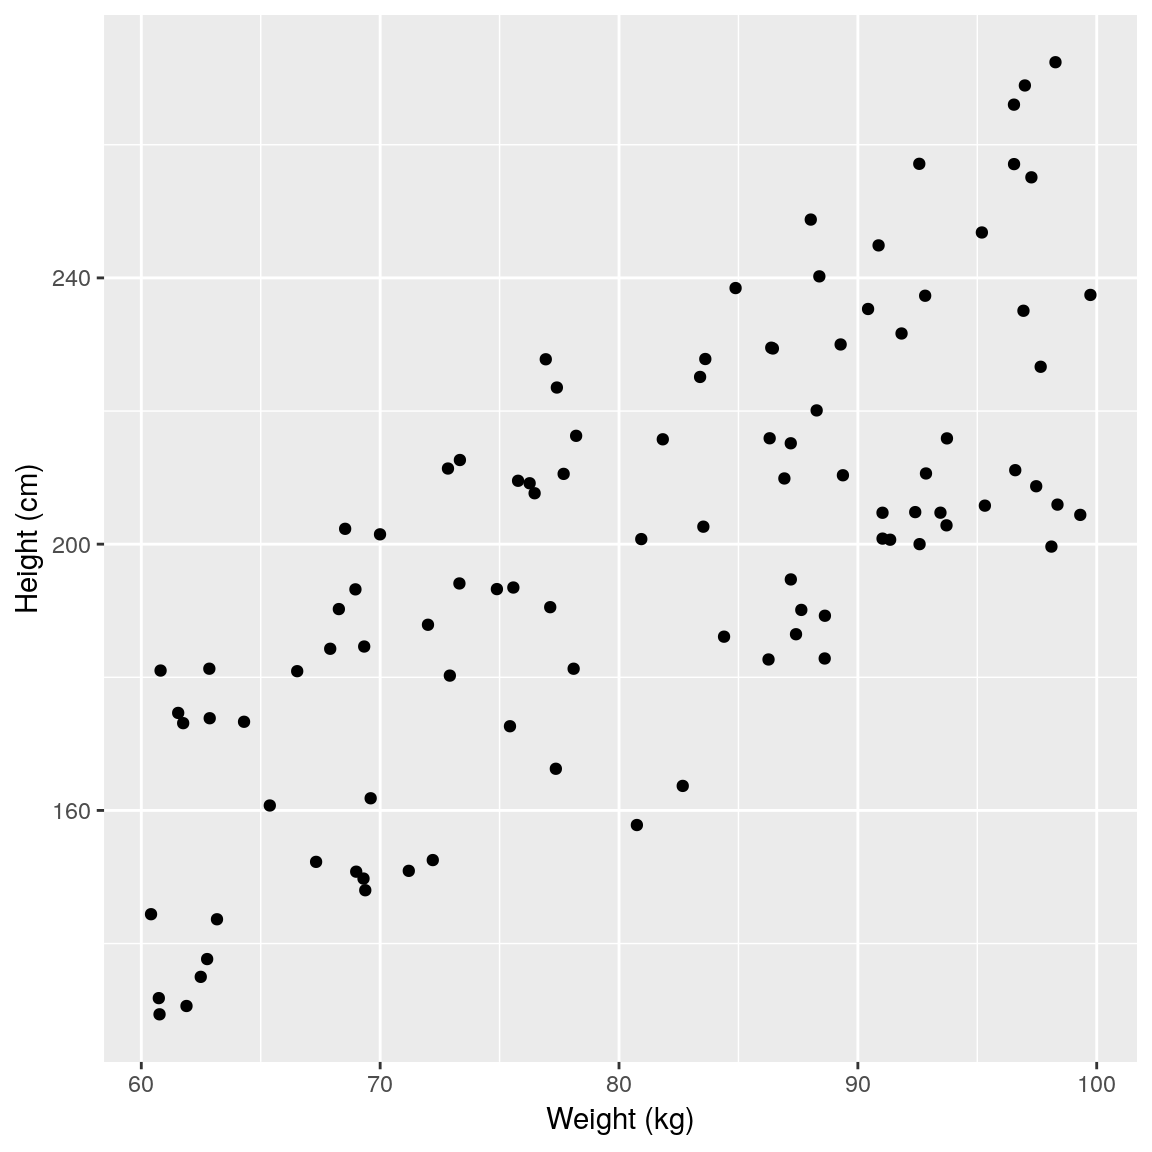
\includegraphics{_main_files/figure-latex/unnamed-chunk-198-1} \end{center}

\eblockST
\emp
\hspace{0.01\textwidth} \bmp\bblockST{\texttt{tidyverse}}

\begin{Shaded}
\begin{Highlighting}[]
\KeywordTok{ggplot}\NormalTok{(df) }\OperatorTok{+}\StringTok{ }
\StringTok{    }\KeywordTok{geom_point}\NormalTok{(}
        \KeywordTok{aes}\NormalTok{(}\DataTypeTok{x =}\NormalTok{ weight, }\DataTypeTok{y =}\NormalTok{ height)) }\OperatorTok{+}
\StringTok{    }\KeywordTok{xlab}\NormalTok{(}\StringTok{"Weight (kg)"}\NormalTok{) }\OperatorTok{+}\StringTok{ }
\StringTok{    }\KeywordTok{ylab}\NormalTok{(}\StringTok{"Height (cm)"}\NormalTok{)}
\end{Highlighting}
\end{Shaded}

\begin{center}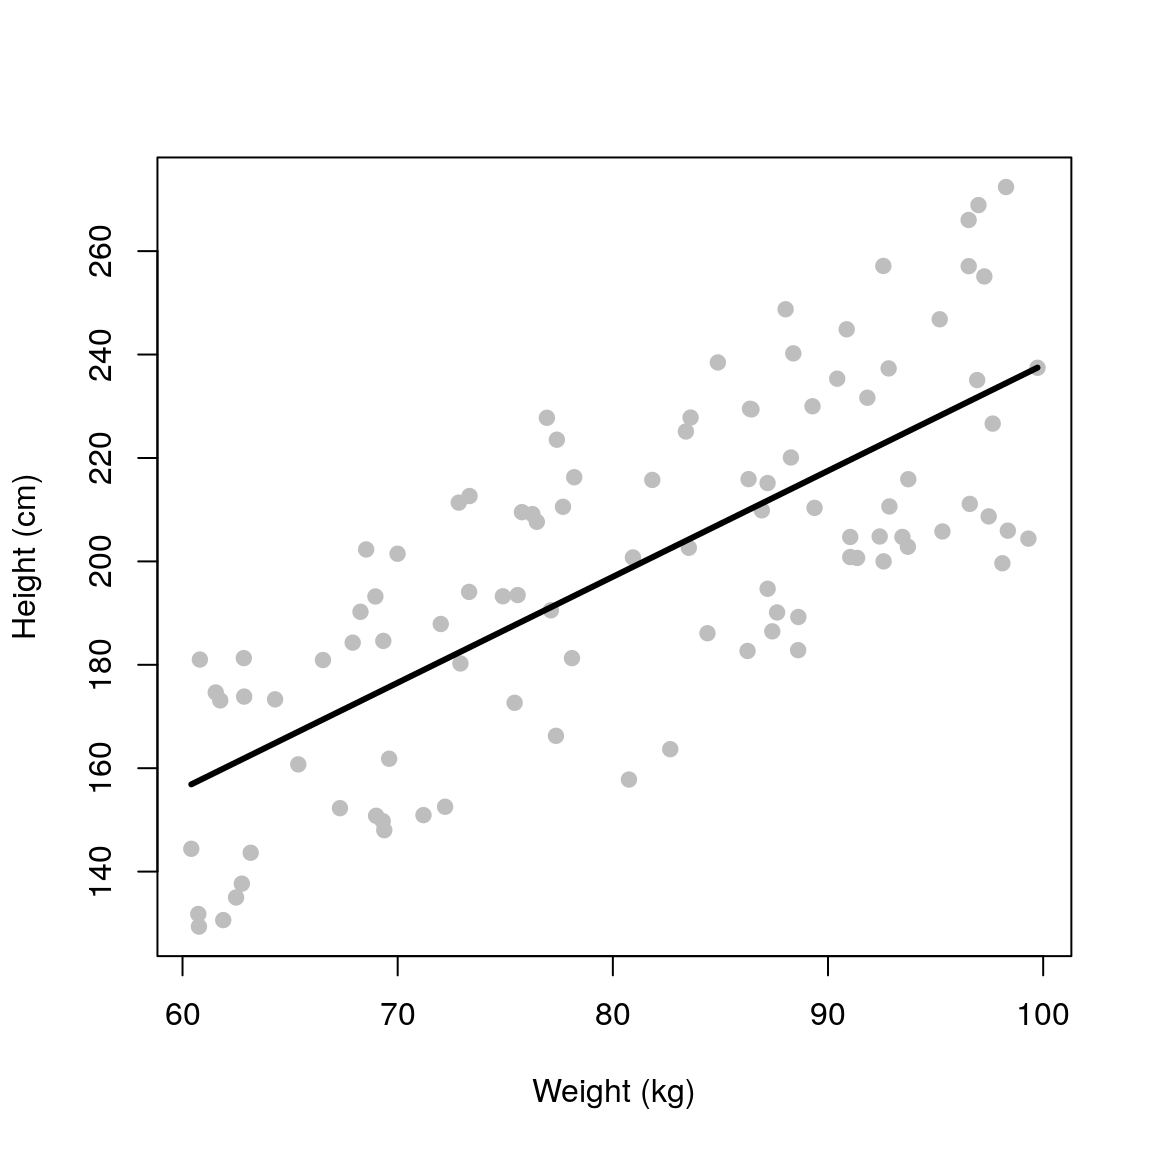
\includegraphics{_main_files/figure-latex/unnamed-chunk-199-1} \end{center}

\eblockST
\emp

\newpage

Data looks similar as before, albeit with a larger variation. We can fit
a model as we have done before and assess the relationship between
\texttt{height} and \texttt{weight}.

\begin{Shaded}
\begin{Highlighting}[]
\NormalTok{## Linear model fit}
\NormalTok{fit <-}\StringTok{ }\KeywordTok{lm}\NormalTok{(height }\OperatorTok{~}\StringTok{ }\NormalTok{weight, }\DataTypeTok{data=}\NormalTok{df)}
\end{Highlighting}
\end{Shaded}

\bmp
\bblockST{Base R}

\begin{Shaded}
\begin{Highlighting}[]
\NormalTok{## predictions}
\NormalTok{newdata <-}\StringTok{ }\KeywordTok{data.frame}\NormalTok{(}
    \DataTypeTok{weight =} \KeywordTok{seq}\NormalTok{(}\KeywordTok{min}\NormalTok{(df}\OperatorTok{$}\NormalTok{weight), }
        \KeywordTok{max}\NormalTok{(df}\OperatorTok{$}\NormalTok{weight), }\DataTypeTok{length.out =} \DecValTok{50}\NormalTok{))}
\NormalTok{newdata}\OperatorTok{$}\NormalTok{height <-}\StringTok{ }\KeywordTok{predict}\NormalTok{(fit, newdata)}

\NormalTok{## Plot model fit}
\KeywordTok{plot}\NormalTok{(height }\OperatorTok{~}\StringTok{ }\NormalTok{weight, }\DataTypeTok{data =}\NormalTok{ df, }
     \DataTypeTok{pch=}\DecValTok{19}\NormalTok{, }\DataTypeTok{xlab=}\StringTok{'Weight (kg)'}\NormalTok{, }
     \DataTypeTok{ylab=}\StringTok{'Height (cm)'}\NormalTok{, }\DataTypeTok{col=}\StringTok{'grey'}\NormalTok{)}
\KeywordTok{lines}\NormalTok{(height }\OperatorTok{~}\StringTok{ }\NormalTok{weight, }\DataTypeTok{data =}\NormalTok{ newdata, }
     \DataTypeTok{col=}\StringTok{'black'}\NormalTok{, }\DataTypeTok{lwd=}\DecValTok{3}\NormalTok{)}
\end{Highlighting}
\end{Shaded}

\begin{center}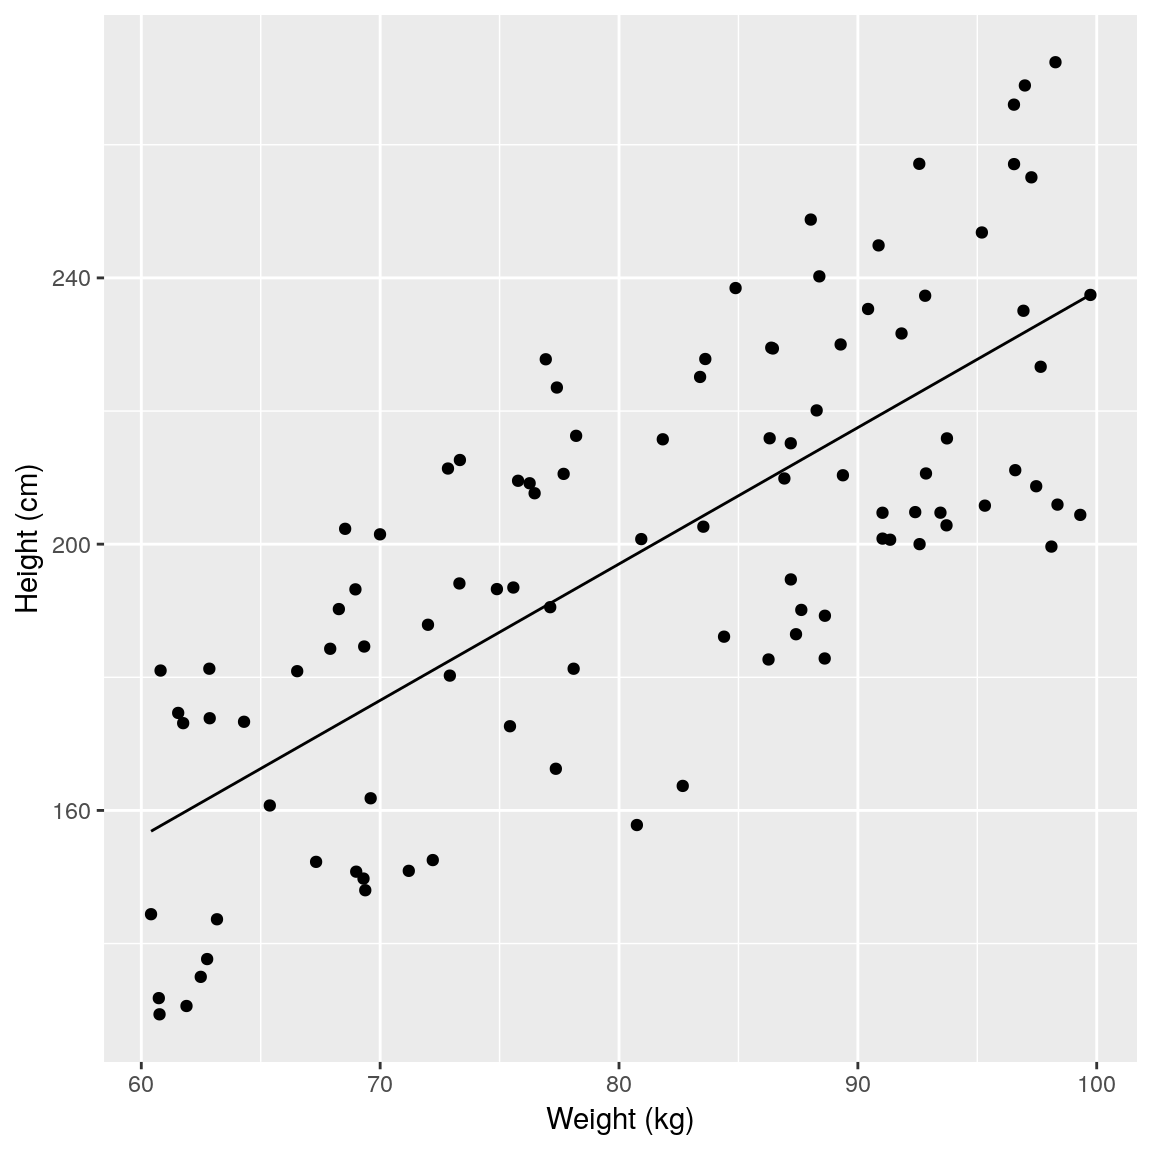
\includegraphics{_main_files/figure-latex/unnamed-chunk-200-1} \end{center}

\eblockST
\emp
\hspace{0.01\textwidth} \bmp\bblockST{\texttt{tidyverse}}

\begin{Shaded}
\begin{Highlighting}[]
\NormalTok{## plot model fit}
\NormalTok{newdata <-}\StringTok{ }\KeywordTok{data.frame}\NormalTok{(}
    \DataTypeTok{weight =} \KeywordTok{seq}\NormalTok{(}\KeywordTok{min}\NormalTok{(df}\OperatorTok{$}\NormalTok{weight), }
        \KeywordTok{max}\NormalTok{(df}\OperatorTok{$}\NormalTok{weight), }\DataTypeTok{length.out =} \DecValTok{50}\NormalTok{))}
\NormalTok{newdata <-}\StringTok{ }\KeywordTok{mutate}\NormalTok{(newdata, }
    \DataTypeTok{height =} \KeywordTok{predict}\NormalTok{(fit, newdata))}
\KeywordTok{ggplot}\NormalTok{(}\DataTypeTok{mapping =} 
        \KeywordTok{aes}\NormalTok{(}\DataTypeTok{x =}\NormalTok{ weight, }\DataTypeTok{y =}\NormalTok{ height)) }\OperatorTok{+}\StringTok{ }
\StringTok{    }\KeywordTok{geom_point}\NormalTok{(}\DataTypeTok{data =}\NormalTok{ df) }\OperatorTok{+}
\StringTok{    }\KeywordTok{geom_line}\NormalTok{(}\DataTypeTok{data =}\NormalTok{ newdata) }\OperatorTok{+}
\StringTok{    }\KeywordTok{xlab}\NormalTok{(}\StringTok{"Weight (kg)"}\NormalTok{) }\OperatorTok{+}\StringTok{ }
\StringTok{    }\KeywordTok{ylab}\NormalTok{(}\StringTok{"Height (cm)"}\NormalTok{)}
\end{Highlighting}
\end{Shaded}

\begin{center}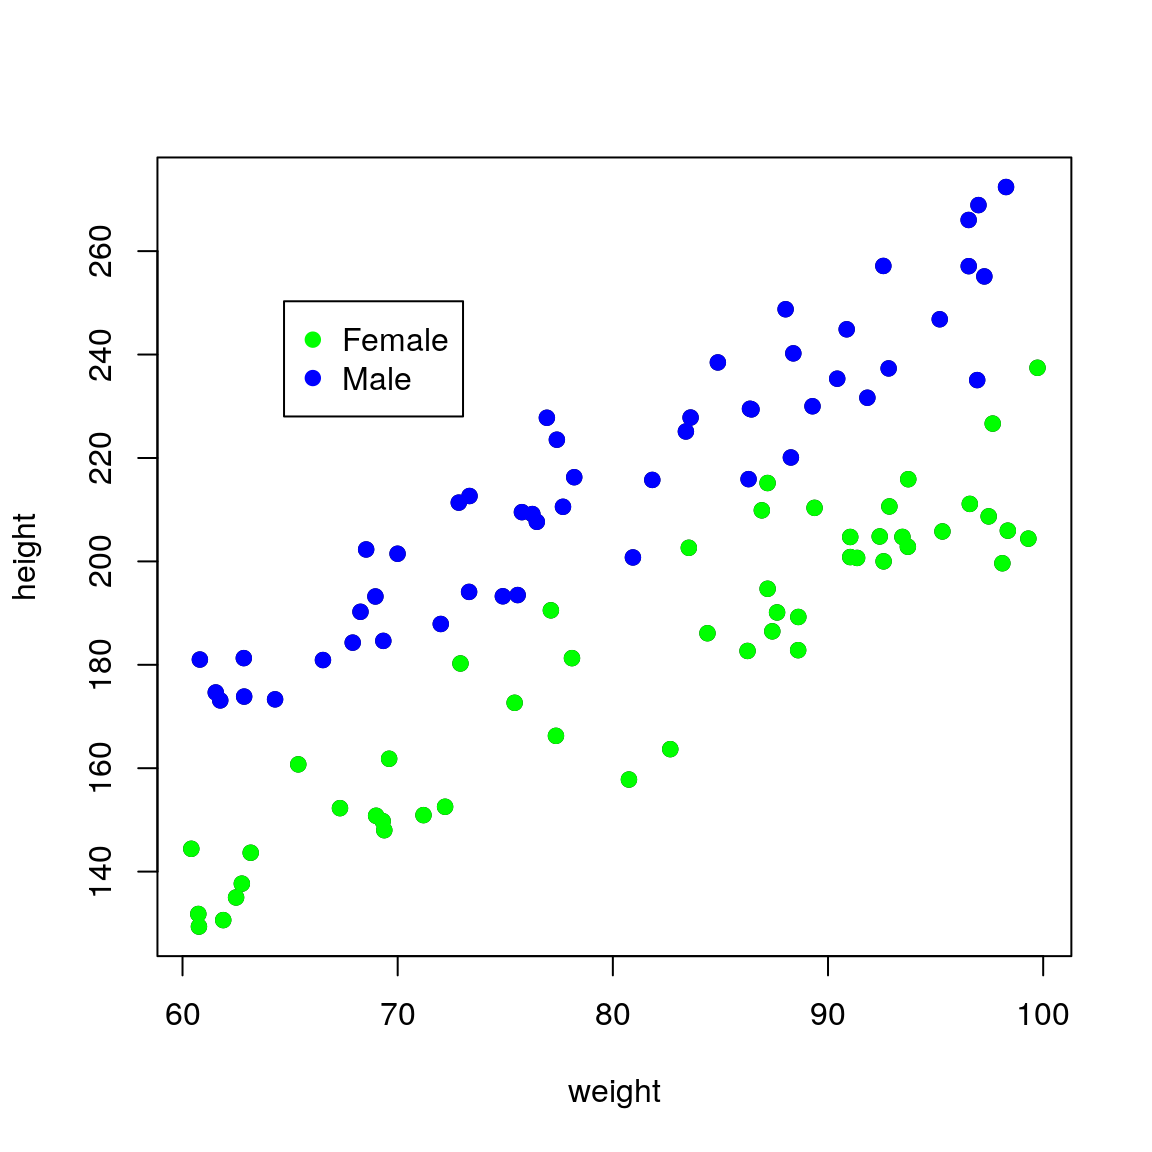
\includegraphics{_main_files/figure-latex/unnamed-chunk-201-1} \end{center}

\eblockST
\emp

\newpage

\begin{Shaded}
\begin{Highlighting}[]
\NormalTok{## Print result}
\KeywordTok{summary}\NormalTok{(fit)}
\end{Highlighting}
\end{Shaded}

\begin{verbatim}
## 
## Call:
## lm(formula = height ~ weight, data = df)
## 
## Residuals:
##     Min      1Q  Median      3Q     Max 
## -40.753 -20.526   2.579  18.889  37.925 
## 
## Coefficients:
##             Estimate Std. Error t value Pr(>|t|)    
## (Intercept)  33.0877    15.2188   2.174   0.0321 *  
## weight        2.0493     0.1859  11.024   <2e-16 ***
## ---
## Signif. codes:  0 '***' 0.001 '**' 0.01 '*' 0.05 '.' 0.1 ' ' 1
## 
## Residual standard error: 22.08 on 98 degrees of freedom
## Multiple R-squared:  0.5536, Adjusted R-squared:  0.549 
## F-statistic: 121.5 on 1 and 98 DF,  p-value: < 2.2e-16
\end{verbatim}

If we colour the data by sex it becomes obvious that this extra
variation is due to sex.

\bmp
\bblockST{Base R}

\begin{Shaded}
\begin{Highlighting}[]
\KeywordTok{plot}\NormalTok{(height }\OperatorTok{~}\StringTok{ }\NormalTok{weight, }\DataTypeTok{data =}\NormalTok{ df, }
     \DataTypeTok{pch =} \DecValTok{19}\NormalTok{)}
\KeywordTok{points}\NormalTok{(height }\OperatorTok{~}\StringTok{ }\NormalTok{weight, }
       \DataTypeTok{pch =} \DecValTok{19}\NormalTok{, }
       \DataTypeTok{data =}\NormalTok{ df[df}\OperatorTok{$}\NormalTok{sex }\OperatorTok{==}\StringTok{ "Female"}\NormalTok{, ], }
       \DataTypeTok{col =} \StringTok{"green"}\NormalTok{)}
\KeywordTok{points}\NormalTok{(height }\OperatorTok{~}\StringTok{ }\NormalTok{weight, }
       \DataTypeTok{pch =} \DecValTok{19}\NormalTok{, }
       \DataTypeTok{data =}\NormalTok{ df[df}\OperatorTok{$}\NormalTok{sex }\OperatorTok{==}\StringTok{ "Male"}\NormalTok{, ], }
       \DataTypeTok{col =} \StringTok{"blue"}\NormalTok{)}
\KeywordTok{legend}\NormalTok{(}\KeywordTok{par}\NormalTok{(}\StringTok{"usr"}\NormalTok{)[}\DecValTok{1}\NormalTok{] }\OperatorTok{*}\StringTok{ }\FloatTok{1.1}\NormalTok{, }
       \KeywordTok{par}\NormalTok{(}\StringTok{"usr"}\NormalTok{)[}\DecValTok{4}\NormalTok{] }\OperatorTok{*}\StringTok{ }\FloatTok{0.9}\NormalTok{,}
       \DataTypeTok{legend =} \KeywordTok{c}\NormalTok{(}\StringTok{"Female"}\NormalTok{, }\StringTok{"Male"}\NormalTok{),}
       \DataTypeTok{pch =} \KeywordTok{c}\NormalTok{(}\DecValTok{19}\NormalTok{, }\DecValTok{19}\NormalTok{),}
       \DataTypeTok{col =} \KeywordTok{c}\NormalTok{(}\StringTok{"green"}\NormalTok{, }\StringTok{"blue"}\NormalTok{))}
\end{Highlighting}
\end{Shaded}

\begin{center}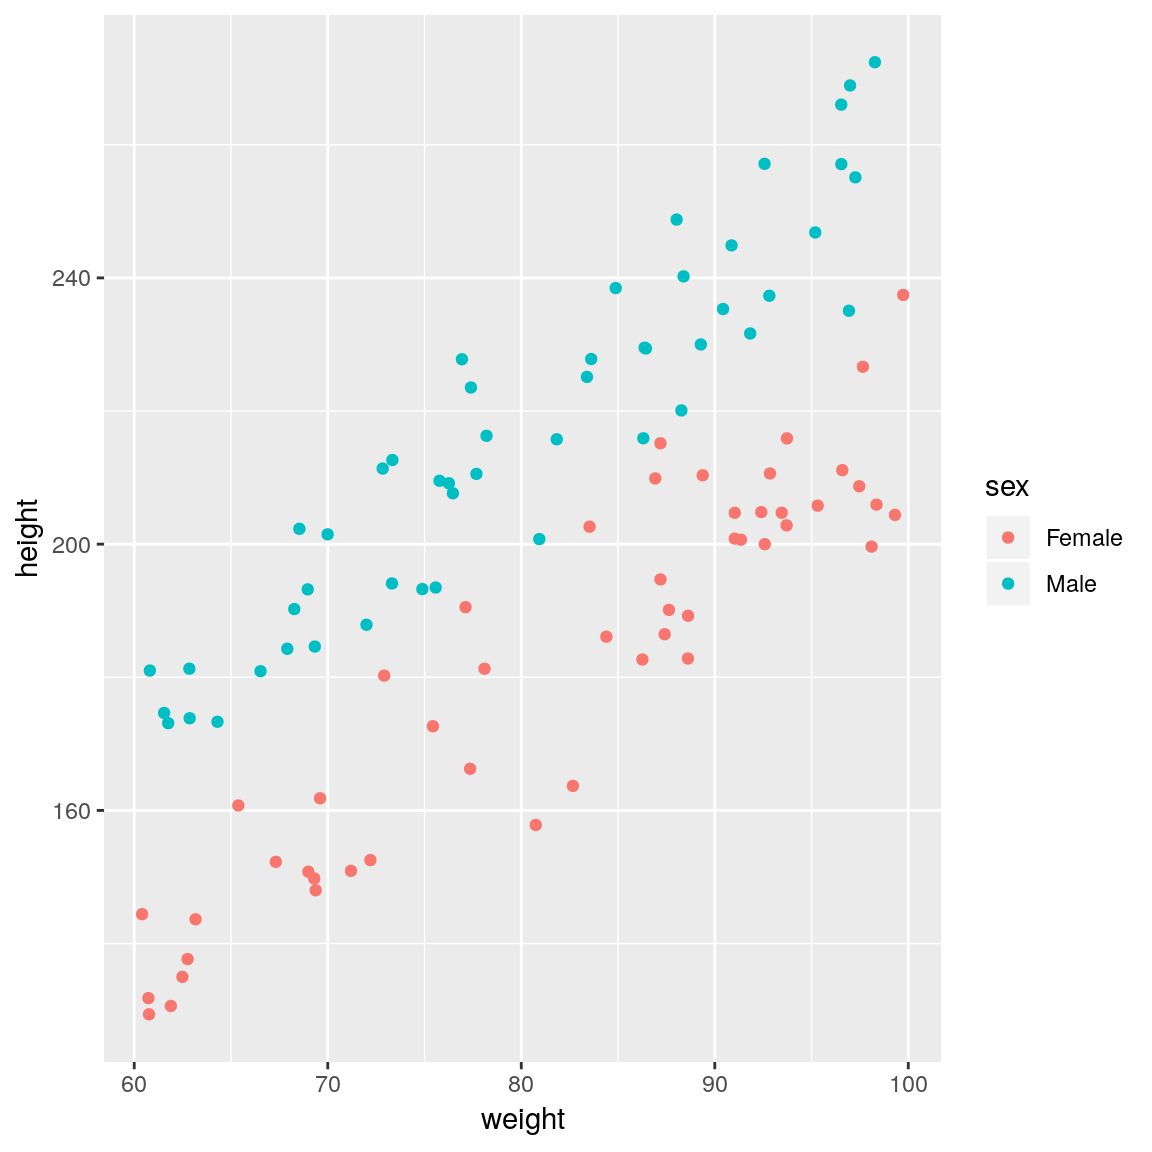
\includegraphics[width=0.6\linewidth]{_main_files/figure-latex/unnamed-chunk-202-1} \end{center}

\eblockST
\emp
\hspace{0.01\textwidth} \bmp\bblockST{\texttt{tidyverse}}

\begin{Shaded}
\begin{Highlighting}[]
\KeywordTok{ggplot}\NormalTok{(df, }
       \KeywordTok{aes}\NormalTok{(}\DataTypeTok{x =}\NormalTok{ weight, }\DataTypeTok{y =}\NormalTok{ height, }
           \DataTypeTok{colour =}\NormalTok{ sex)) }\OperatorTok{+}
\StringTok{    }\KeywordTok{geom_point}\NormalTok{()}
\end{Highlighting}
\end{Shaded}

\begin{center}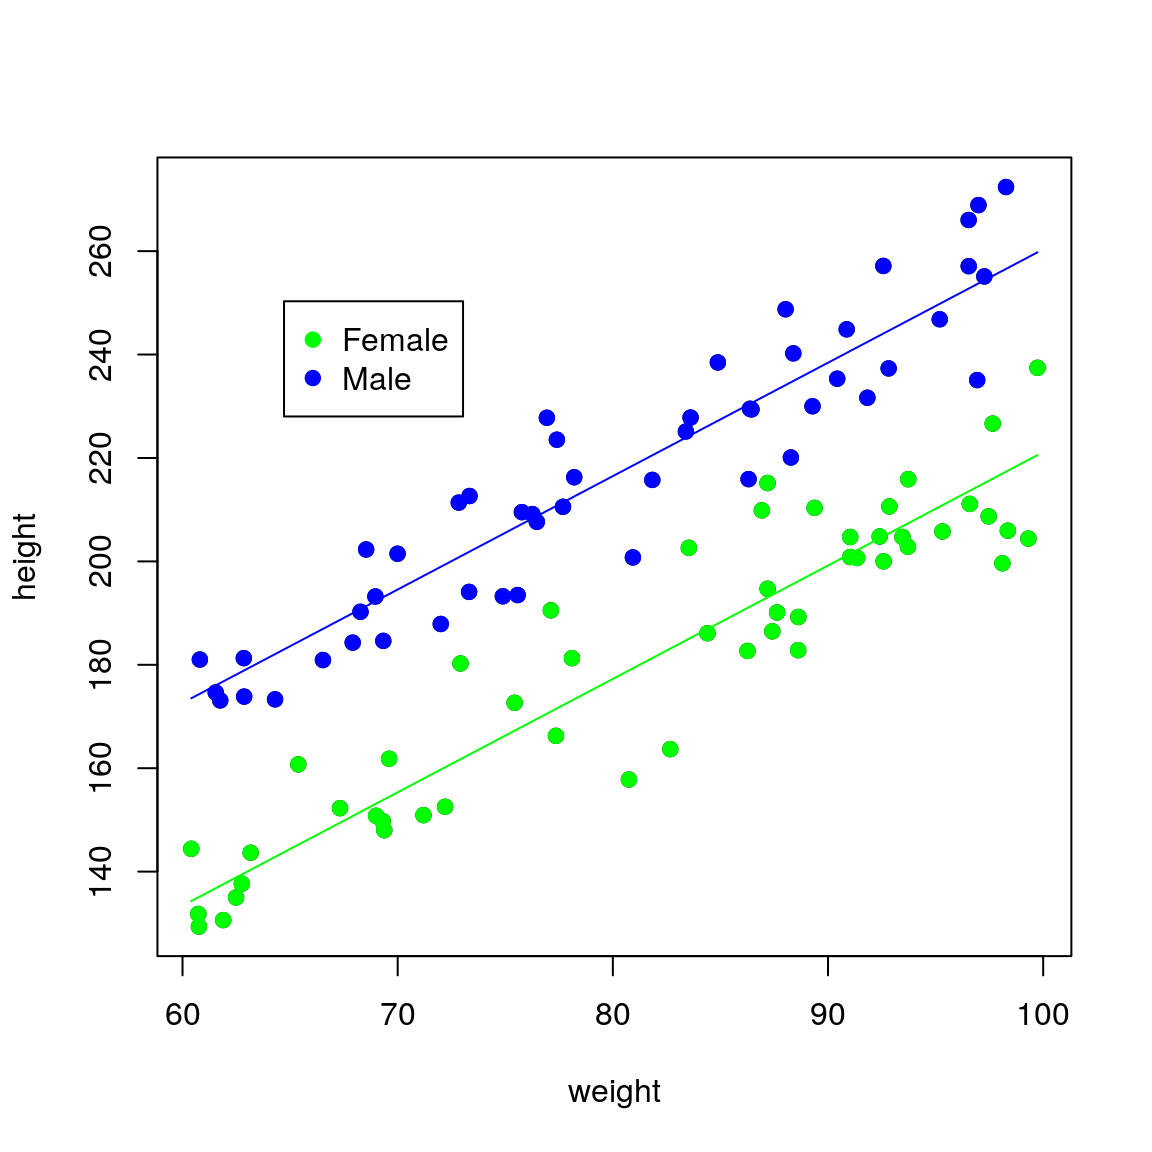
\includegraphics{_main_files/figure-latex/unnamed-chunk-203-1} \end{center}

\eblockST
\emp

\newpage

\texttt{sex} is an important covariate and should therefore be added to
the model. That is, we need a model that has different regression lines
for each sex. The \emph{syntax} for the R formula remains exactly the
same
\texttt{response\ \textasciitilde{}\ explanatory\_1\ +\ ...\ +\ explanatory\_p},
but behind the scenes categorical variables are treated differently to
continuous variables.

To cope with categorical variables (known as \textbf{factors} in R's
lingo), we introduce a \textbf{dummy} variable.

\[
S_i = \left\{\begin{array}{ll}
        1 & \mbox{if $i$ is male},\\
        0 & \mbox{otherwise}
        \end{array}
        \right.
\]

Here, female is known as the \textbf{baseline}/\textbf{reference level}

The regression is:

\[
y_i = \beta_0 + \beta_1 S_i + \beta_2 x_i + \epsilon_i
\] Or in English:

\[
\begin{aligned}
\mathrm{height}_i & = \beta_0 + \beta_1\mathrm{sex}_i + \beta_2\mathrm{weight}_i + \epsilon_i \\
\end{aligned}
\] Where \texttt{sex} is the dummy variable \texttt{S\_i} that can take
the value of 0 (female) or 1 (male)

The mean regression lines for male and female now look like this:

\begin{itemize}
\tightlist
\item
  \textbf{Female} (\texttt{sex=0})
\end{itemize}

\[
\begin{aligned}
    \mathrm{height}_i & = \beta_0 + (\beta_1 \times 0) + \beta_2\mathrm{weight}_i\\
    \mathrm{height}_i & = \beta_0 + \beta_2\mathrm{weight}_i
\end{aligned}
\]

\begin{itemize}
\tightlist
\item
  \textbf{Male} (\texttt{sex=1})
\end{itemize}

\[
\begin{aligned}
    \mathrm{height}_i & = \beta_0 + (\beta_1 \times 1) + \beta_2\mathrm{weight}_i\\
    \mathrm{height}_i & = (\beta_0 + \beta_1) + \beta_2\mathrm{weight}_i
\end{aligned}
\] By introducing a dummy variable, we have now simplified the problem
into \textbf{two} regression lines, where the \textbf{intercept} is:

\begin{itemize}
\tightlist
\item
  \textbf{Female}: \(\beta_0\)
\item
  \textbf{Male}: \(\beta_0 + \beta_1\)
\end{itemize}

Whilst the \textbf{gradient} is \(\beta_2\) in both cases.

\begin{Shaded}
\begin{Highlighting}[]
\NormalTok{## Linear model fit}
\NormalTok{fit <-}\StringTok{ }\KeywordTok{lm}\NormalTok{(height }\OperatorTok{~}\StringTok{ }\NormalTok{sex }\OperatorTok{+}\StringTok{ }\NormalTok{weight, }\DataTypeTok{data=}\NormalTok{df)}
\end{Highlighting}
\end{Shaded}

\newpage

\begin{Shaded}
\begin{Highlighting}[]
\NormalTok{## Print result}
\KeywordTok{summary}\NormalTok{(fit)}
\end{Highlighting}
\end{Shaded}

\begin{verbatim}
## 
## Call:
## lm(formula = height ~ sex + weight, data = df)
## 
## Residuals:
##     Min      1Q  Median      3Q     Max 
## -21.106  -6.853  -1.162   6.691  22.111 
## 
## Coefficients:
##             Estimate Std. Error t value Pr(>|t|)    
## (Intercept)   1.8269     7.0411   0.259    0.796    
## sexMale      39.2220     1.9976  19.634   <2e-16 ***
## weight        2.1931     0.0841  26.078   <2e-16 ***
## ---
## Signif. codes:  0 '***' 0.001 '**' 0.01 '*' 0.05 '.' 0.1 ' ' 1
## 
## Residual standard error: 9.95 on 97 degrees of freedom
## Multiple R-squared:  0.9103, Adjusted R-squared:  0.9084 
## F-statistic: 491.9 on 2 and 97 DF,  p-value: < 2.2e-16
\end{verbatim}

The \texttt{sexMale} coefficient is \(\beta_1\) in the equations above
and it represents the \emph{difference} in intercept between males and
females (remember that the gradient is the same for both sexes). Thus
for the \emph{same} weight, men on average will be \texttt{sexMale}=39.2
cm taller than females.

To plot the fitted lines, we can use a similar trick using
\texttt{predict()} as \protect\hyperlink{sec:prediction}{before}. This
time we need to produce predictions using all relevant combinations of
explanatory variables: \texttt{weight} and \texttt{sex} in this case. A
useful function to do this is \texttt{expand.grid()}:

\newpage

\bmp
\bblockST{Base R}

\begin{Shaded}
\begin{Highlighting}[]
\NormalTok{## create dataset to predict to}
\NormalTok{newdata <-}\StringTok{ }\KeywordTok{expand.grid}\NormalTok{(}
    \DataTypeTok{weight =} \KeywordTok{seq}\NormalTok{(}\KeywordTok{min}\NormalTok{(df}\OperatorTok{$}\NormalTok{weight), }
        \KeywordTok{max}\NormalTok{(df}\OperatorTok{$}\NormalTok{weight), }\DataTypeTok{length.out =} \DecValTok{50}\NormalTok{),}
    \DataTypeTok{sex =} \KeywordTok{c}\NormalTok{(}\StringTok{"Female"}\NormalTok{, }\StringTok{"Male"}\NormalTok{))}

\NormalTok{## generate predictions}
\NormalTok{newdata <-}\StringTok{ }\KeywordTok{cbind}\NormalTok{(newdata, }
    \DataTypeTok{height =} \KeywordTok{predict}\NormalTok{(fit, newdata))}

\NormalTok{## plot fitted lines against the data}
\KeywordTok{plot}\NormalTok{(height }\OperatorTok{~}\StringTok{ }\NormalTok{weight, }\DataTypeTok{data =}\NormalTok{ df, }
    \DataTypeTok{pch =} \DecValTok{19}\NormalTok{)}
\KeywordTok{points}\NormalTok{(height }\OperatorTok{~}\StringTok{ }\NormalTok{weight, }
    \DataTypeTok{pch =} \DecValTok{19}\NormalTok{, }
    \DataTypeTok{data =}\NormalTok{ df[df}\OperatorTok{$}\NormalTok{sex }\OperatorTok{==}\StringTok{ "Female"}\NormalTok{, ], }
    \DataTypeTok{col =} \StringTok{"green"}\NormalTok{)}
\KeywordTok{points}\NormalTok{(height }\OperatorTok{~}\StringTok{ }\NormalTok{weight, }
    \DataTypeTok{pch =} \DecValTok{19}\NormalTok{, }
    \DataTypeTok{data =}\NormalTok{ df[df}\OperatorTok{$}\NormalTok{sex }\OperatorTok{==}\StringTok{ "Male"}\NormalTok{, ], }
    \DataTypeTok{col =} \StringTok{"blue"}\NormalTok{)}
\KeywordTok{lines}\NormalTok{(height }\OperatorTok{~}\StringTok{ }\NormalTok{weight, }
    \DataTypeTok{data =}\NormalTok{ newdata[}
\NormalTok{        newdata}\OperatorTok{$}\NormalTok{sex }\OperatorTok{==}\StringTok{ "Female"}\NormalTok{, ], }
    \DataTypeTok{col =} \StringTok{"green"}\NormalTok{)}
\KeywordTok{lines}\NormalTok{(height }\OperatorTok{~}\StringTok{ }\NormalTok{weight, }
    \DataTypeTok{data =}\NormalTok{ newdata[}
\NormalTok{        newdata}\OperatorTok{$}\NormalTok{sex }\OperatorTok{==}\StringTok{ "Male"}\NormalTok{, ], }
    \DataTypeTok{col =} \StringTok{"blue"}\NormalTok{)}
\KeywordTok{legend}\NormalTok{(}\KeywordTok{par}\NormalTok{(}\StringTok{"usr"}\NormalTok{)[}\DecValTok{1}\NormalTok{] }\OperatorTok{*}\StringTok{ }\FloatTok{1.1}\NormalTok{, }
    \KeywordTok{par}\NormalTok{(}\StringTok{"usr"}\NormalTok{)[}\DecValTok{4}\NormalTok{] }\OperatorTok{*}\StringTok{ }\FloatTok{0.9}\NormalTok{,}
    \DataTypeTok{legend =} \KeywordTok{c}\NormalTok{(}\StringTok{"Female"}\NormalTok{, }\StringTok{"Male"}\NormalTok{),}
    \DataTypeTok{pch =} \KeywordTok{c}\NormalTok{(}\DecValTok{19}\NormalTok{, }\DecValTok{19}\NormalTok{),}
    \DataTypeTok{col =} \KeywordTok{c}\NormalTok{(}\StringTok{"green"}\NormalTok{, }\StringTok{"blue"}\NormalTok{))}
\end{Highlighting}
\end{Shaded}

\begin{center}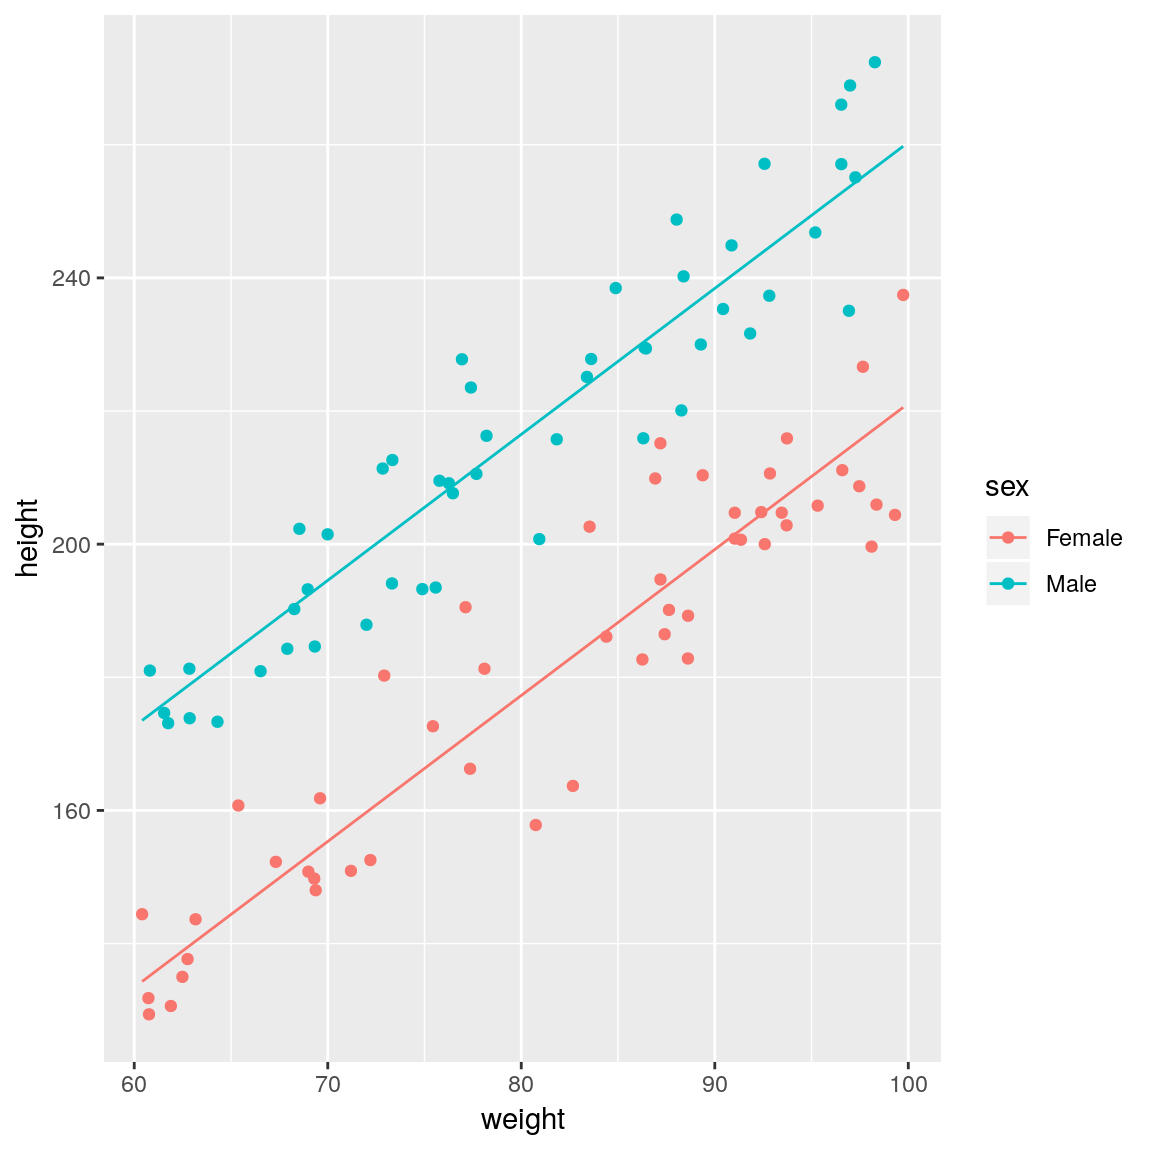
\includegraphics[width=0.6\linewidth]{_main_files/figure-latex/unnamed-chunk-204-1} \end{center}

\eblockST
\emp
\hspace{0.01\textwidth} \bmp\bblockST{\texttt{tidyverse}}

\begin{Shaded}
\begin{Highlighting}[]
\NormalTok{## create dataset to predict to}
\NormalTok{newdata <-}\StringTok{ }\KeywordTok{expand.grid}\NormalTok{(}
    \DataTypeTok{weight =} \KeywordTok{seq}\NormalTok{(}\KeywordTok{min}\NormalTok{(df}\OperatorTok{$}\NormalTok{weight), }
        \KeywordTok{max}\NormalTok{(df}\OperatorTok{$}\NormalTok{weight), }\DataTypeTok{length.out =} \DecValTok{50}\NormalTok{),}
    \DataTypeTok{sex =} \KeywordTok{c}\NormalTok{(}\StringTok{"Female"}\NormalTok{, }\StringTok{"Male"}\NormalTok{))}

\NormalTok{## generate predictions}
\NormalTok{newdata <-}\StringTok{ }\KeywordTok{mutate}\NormalTok{(newdata, }
    \DataTypeTok{height =} \KeywordTok{predict}\NormalTok{(fit, newdata))}

\NormalTok{## plot fitted lines against the data}
\KeywordTok{ggplot}\NormalTok{(}\DataTypeTok{mapping =} 
        \KeywordTok{aes}\NormalTok{(}\DataTypeTok{x =}\NormalTok{ weight, }\DataTypeTok{y =}\NormalTok{ height, }
            \DataTypeTok{colour =}\NormalTok{ sex)) }\OperatorTok{+}
\StringTok{    }\KeywordTok{geom_point}\NormalTok{(}\DataTypeTok{data =}\NormalTok{ df) }\OperatorTok{+}
\StringTok{    }\KeywordTok{geom_line}\NormalTok{(}\DataTypeTok{data =}\NormalTok{ newdata)}
\end{Highlighting}
\end{Shaded}

\begin{center}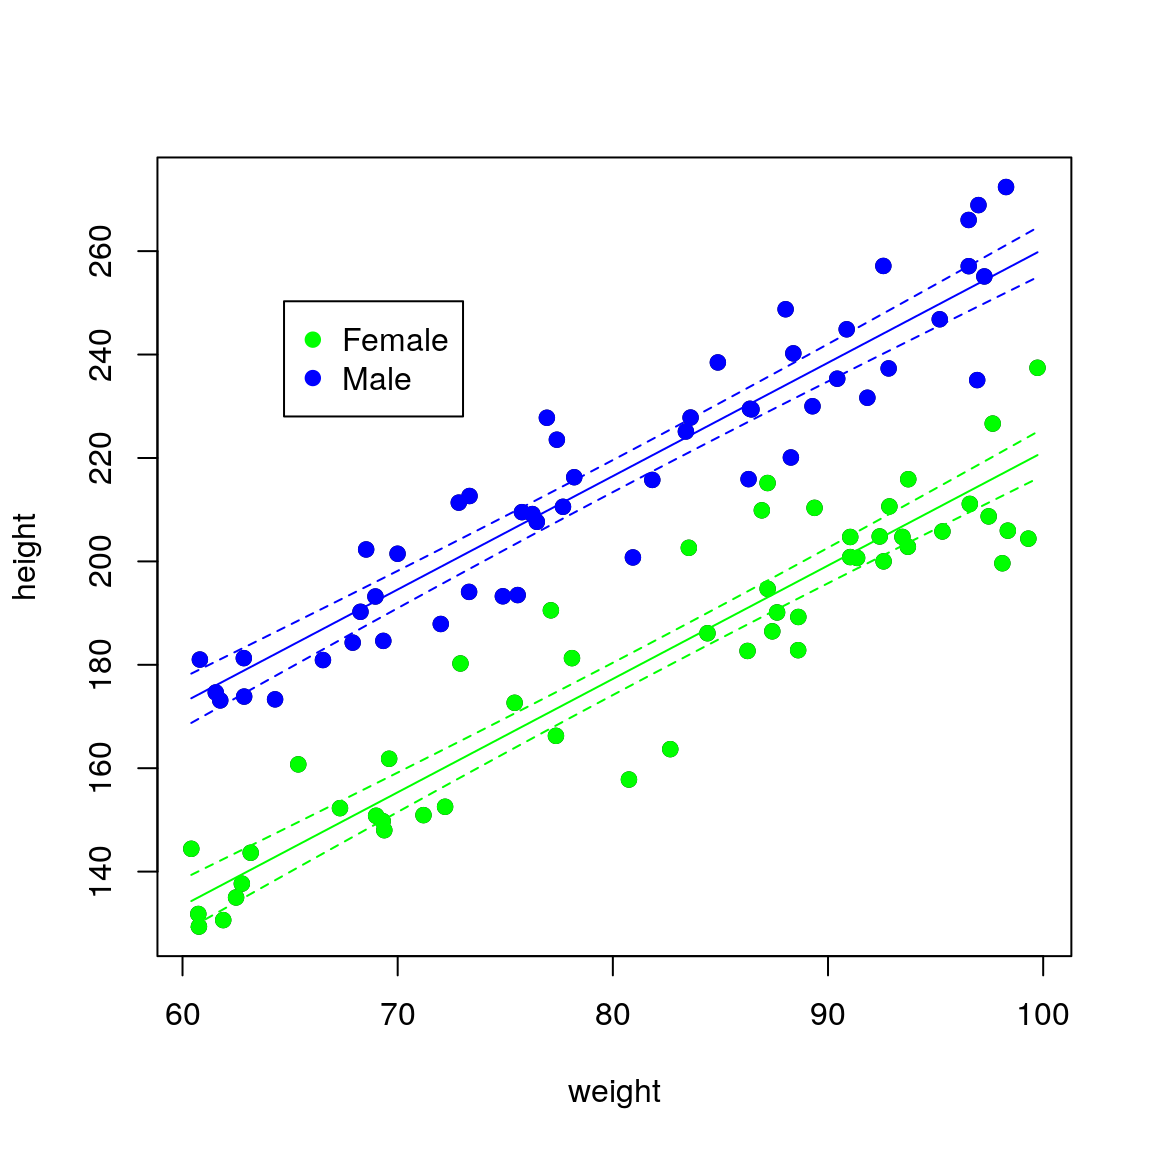
\includegraphics{_main_files/figure-latex/unnamed-chunk-205-1} \end{center}

\eblockST
\emp

\newpage

\hypertarget{tsk5}{}\bblockT[Task]{\phantomsection\label{sol5}5}

Add 97\% confidence intervals to the fitted lines plots above. \eblockT

\hyperlink{sol5}{\buttonS{Show Solution on P\colpageref{tsk5}}}

\hypertarget{tsk6}{}\bblockT[Task]{\phantomsection\label{sol6}6}

Compare the total variation explained by the model with just weight to
the one which considers weight \emph{and} sex. What gives rise to this
difference?

\eblockT

\hyperlink{sol6}{\buttonS{Show Solution on P\colpageref{tsk6}}}

\textbf{Note} the baseline/reference level in R is automatically taken
to be the \emph{first} factor level.

\begin{Shaded}
\begin{Highlighting}[]
\KeywordTok{levels}\NormalTok{(df}\OperatorTok{$}\NormalTok{sex)}
\end{Highlighting}
\end{Shaded}

\begin{verbatim}
## [1] "Female" "Male"
\end{verbatim}

We can change this by re-ordering the levels if we wanted to.

\begin{Shaded}
\begin{Highlighting}[]
\NormalTok{df}\OperatorTok{$}\NormalTok{sex <-}\StringTok{ }\KeywordTok{factor}\NormalTok{(df}\OperatorTok{$}\NormalTok{sex, }\DataTypeTok{levels =} \KeywordTok{c}\NormalTok{(}\StringTok{'Male'}\NormalTok{, }\StringTok{'Female'}\NormalTok{))}
\end{Highlighting}
\end{Shaded}

\begin{Shaded}
\begin{Highlighting}[]
\NormalTok{## Linear model fit}
\NormalTok{fit <-}\StringTok{ }\KeywordTok{lm}\NormalTok{(height }\OperatorTok{~}\StringTok{ }\NormalTok{sex }\OperatorTok{+}\StringTok{ }\NormalTok{weight, }\DataTypeTok{data=}\NormalTok{df)}

\NormalTok{## Print result}
\KeywordTok{summary}\NormalTok{(fit)}
\end{Highlighting}
\end{Shaded}

\begin{verbatim}
## 
## Call:
## lm(formula = height ~ sex + weight, data = df)
## 
## Residuals:
##     Min      1Q  Median      3Q     Max 
## -21.106  -6.853  -1.162   6.691  22.111 
## 
## Coefficients:
##             Estimate Std. Error t value Pr(>|t|)    
## (Intercept)  41.0489     6.8707   5.975 3.81e-08 ***
## sexFemale   -39.2220     1.9976 -19.634  < 2e-16 ***
## weight        2.1931     0.0841  26.078  < 2e-16 ***
## ---
## Signif. codes:  0 '***' 0.001 '**' 0.01 '*' 0.05 '.' 0.1 ' ' 1
## 
## Residual standard error: 9.95 on 97 degrees of freedom
## Multiple R-squared:  0.9103, Adjusted R-squared:  0.9084 
## F-statistic: 491.9 on 2 and 97 DF,  p-value: < 2.2e-16
\end{verbatim}

As expected this change simply changes the sign of the \(\beta_1\)
parameter, because the dummy variable now takes the value of 0 for male
and 1 for female (i.e we switched things around).

\newpage

\section{Practical 3}\label{practical-3}

We will use the fruitfly dataset
(\href{https://www.nature.com/articles/294580a0}{Partridge and Farquhar
(1981)}) as we did in the previous practical

\hypertarget{tsk7}{}\bblockT[Task]{\phantomsection\label{sol7}7}

\begin{enumerate}
\def\labelenumi{\arabic{enumi}.}
\tightlist
\item
  Fit a linear model with lifespan as response variable and thorax
  length and type of companion as explanatory variables
\item
  Display a summary of the fit, together with the 97\% confidence
  intervals for the estimated parameters
\item
  Why do we get two parameters for type of companion and what do they
  mean in practice?
\end{enumerate}

\eblockT

\hyperlink{sol7}{\buttonS{Show Solution on P\colpageref{tsk7}}}

\hypertarget{tsk8}{}\bblockT[Task]{\phantomsection\label{sol8}8}

\begin{enumerate}
\def\labelenumi{\arabic{enumi}.}
\setcounter{enumi}{3}
\tightlist
\item
  Plot the mean regression line for each type of companion together with
  the observed data.
\end{enumerate}

\eblockT

\hyperlink{sol8}{\buttonS{Show Solution on P\colpageref{tsk8}}}

\hypertarget{tsk9}{}\bblockT[Task]{\phantomsection\label{sol9}9}

\begin{enumerate}
\def\labelenumi{\arabic{enumi}.}
\setcounter{enumi}{4}
\tightlist
\item
  Show the diagnostic plots for the model, what can you say about the
  model fit?
\item
  Compare the total variation explained by this model with the one that
  only used \texttt{thorax} as a covariate. What can you say about the
  importance of the type of companion?
\end{enumerate}

\eblockT

\hyperlink{sol9}{\buttonS{Show Solution on P\colpageref{tsk9}}}

\section{Practical issues}\label{practical-issues}

The most common issues when trying to fit simple linear regression
models is that our response variable is not normal which violates our
modelling assumption. There are two things we can do in this case:

\begin{enumerate}
\def\labelenumi{\arabic{enumi}.}
\tightlist
\item
  \textbf{Variable transformation}

  \begin{itemize}
  \tightlist
  \item
    Can sometimes fix linearity
  \item
    Can sometimes fix non-normality and heteroscedasticity (i.e
    non-constant variance)
  \end{itemize}
\item
  \textbf{\emph{Generalised} Linear Models (GLMs)} to change the
  \textbf{error} structure (i.e the assumption that residuals need to be
  normal)
\end{enumerate}

\section{Summary}\label{summary-1}

\textbf{Linear regression} is a powerful tool:

\begin{itemize}
\tightlist
\item
  It splits the data into \textbf{signal} (trend / mean), and
  \textbf{noise} (residual error).
\item
  It can cope with \textbf{multiple variables}.
\item
  It can incorporate different \textbf{types} of variable
\item
  It can be used to produce \textbf{point} and \textbf{interval}
  estimates for the parameters.
\item
  It can be used to assess the importance of variables.
\end{itemize}

\textbf{But} always \textbf{check} that the model fit is sensible and
that the results make sense within the context of the problem at hand.
Investigate thoroughly if they do not!!

\chapter{Generalised linear models}\label{generalised-linear-models}

Slides can be downloaded from:

\begin{itemize}
\tightlist
\item
  \href{https://exeter-data-analytics.github.io/StatModelling/03-generalised-linear-models-handout.pdf}{GLMs
  in R}
\end{itemize}

\section{Motivation}\label{motivation-1}

In the previous workshop we have seen that linear models are a powerful
modelling tool. However, we have to satisfy the following assumptions:

\begin{enumerate}
\def\labelenumi{\arabic{enumi}.}
\tightlist
\item
  A \textbf{linear} mean function is relevant.
\item
  Variances are equal across all predicted values of the response
  (\textbf{homoscedatic})
\item
  Errors are \textbf{normally} distributed.
\item
  Samples collected at \textbf{random}.
\item
  Errors are \textbf{independent}.
\end{enumerate}

If assumptions 1--3 are violated we can \emph{transform} our response
variable to try and fix this (power transforms, Tukey's
ladder-of-powers, Box-Cox transformation, Tukey and Mosteller's bulging
rule). However, in a lot of other cases this is either not possible (e.g
binary output) or we want to explicitly model the underlying
distribution (e.g count data). Instead, we can use \emph{Generalised}
Linear Models (GLMs) that let us change the \emph{error structure} of
our data. By error structure we mean the assumption placed on the
\emph{residuals}. In the previous simple linear regression case we
assumed them to be normal (i.e
\(\epsilon_i \sim \mathcal{N}(0,\sigma^2)\))

\section{Generalised Linear Models
(GLMs)}\label{generalised-linear-models-glms}

\textbf{Generalised Linear Models} (GLMs) have:

\begin{enumerate}
\def\labelenumi{\arabic{enumi}.}
\tightlist
\item
  A linear mean (of your making).
\item
  A \textbf{link function} (like an `internal' transformation).
\item
  An \textbf{error structure}.
\end{enumerate}

\subsection{Link functions}\label{link-functions}

A \textbf{link} function \emph{links} your \textbf{\emph{mean}} function
to the scale of the \textbf{observed data} e.g.

\begin{itemize}
\tightlist
\item
  \textbf{Response} variable \(Y\) and explanatory variable(s) \(X\).
\item
  The \textbf{regression} parameters are denoted using \(\beta_p\) as
  before.
\item
  \textbf{Linear} function: \(\beta_0 + \beta_1 X\).
\item
  \(E(Y) = g^{-1}\left(\beta_0 + \beta_1 X\right)\).
\end{itemize}

Here \(E(Y)\) denotes the \textbf{expected value} (i.e.~mean of \(Y\)).

The function \(g(\cdot)\) is known as the \textbf{link function}, and
\(g^{-1}(\cdot)\) denotes the \textbf{inverse} of \(g(\cdot)\).

The simple linear regression model we have used so far is a special
cases of a GLM:

\begin{Shaded}
\begin{Highlighting}[]
\KeywordTok{lm}\NormalTok{(height }\OperatorTok{~}\StringTok{ }\NormalTok{weight)}
\end{Highlighting}
\end{Shaded}

is equivalent to

\begin{Shaded}
\begin{Highlighting}[]
\KeywordTok{glm}\NormalTok{(height }\OperatorTok{~}\StringTok{ }\NormalTok{weight, }\DataTypeTok{family=}\KeywordTok{gaussian}\NormalTok{(}\DataTypeTok{link=}\NormalTok{identity))}
\end{Highlighting}
\end{Shaded}

Compared to
\href{https://www.rdocumentation.org/packages/stats/versions/3.5.1/topics/lm}{\texttt{lm()}},
the
\href{https://www.rdocumentation.org/packages/stats/versions/3.5.1/topics/glm}{\texttt{glm()}}
function takes an additional argument called
\href{https://www.rdocumentation.org/packages/stats/versions/3.5.1/topics/family}{\texttt{family}},
which specifies the error structure \textbf{and} link function.

The default \textbf{link function} for the normal (Gaussian)
distribution is the \textbf{identity}, i.e.~for mean \(\mu\) we have:

\[
\mu = \beta_0 + \beta_1 X
\]

Defaults are usually good choices (shown in bold below):

\begin{longtable}[]{@{}cc@{}}
\toprule
Family & Link\tabularnewline
\midrule
\endhead
\texttt{gaussian} & \textbf{\texttt{identity}}\tabularnewline
\texttt{binomial} & \textbf{\texttt{logit}}, \texttt{probit} or
\texttt{cloglog}\tabularnewline
\texttt{poisson} & \textbf{\texttt{log}}, \texttt{identity} or
\texttt{sqrt}\tabularnewline
\texttt{Gamma} & \textbf{\texttt{inverse}}, \texttt{identity} or
\texttt{log}\tabularnewline
\texttt{inverse.gaussian} & \textbf{\texttt{1/mu\^{}2}}\tabularnewline
\texttt{quasi} & user-defined\tabularnewline
\texttt{quasibinomial} & \textbf{\texttt{logit}}\tabularnewline
\texttt{quasipoisson} & \textbf{\texttt{log}}\tabularnewline
\bottomrule
\end{longtable}

\hypertarget{tsk10}{}\bblockT[Task]{\phantomsection\label{sol10}10}

Using the fruitfly data introduced in
\protect\hyperlink{sec:practical1}{Practical 1}, fit a linear model with
lifespan as response variable and thorax length and type of companion as
explanatory variables using both the \texttt{lm} and \texttt{glm}
functions and compare their summaries. \eblockT

\hyperlink{sol10}{\buttonS{Show Solution on P\colpageref{tsk10}}}

\subsection{Workflow}\label{workflow}

\begin{itemize}
\tightlist
\item
  Exploratory data analysis
\item
  Choose suitable error term
\item
  Choose suitable mean function (and link function)
\item
  Fit model

  \begin{itemize}
  \tightlist
  \item
    Residual checks and model fit diagnostics
  \item
    Revise model (transformations etc.)
  \end{itemize}
\item
  Model simplification if required
\item
  Check final model
\end{itemize}

\section{Poisson regression (for count
data)}\label{poisson-regression-for-count-data}

Count data are ubiquitous in the life sciences (e.g number of parasites
per microlitre of blood, number of species in a particular area). These
type of data are \textbf{discrete} and \textbf{non-negative}. In such
cases assuming our response variable to be normally distributed is not
typically sensible. The Poisson distribution lets us model count data
explicitly.

Recall the simple linear regression case (i.e a GLM with a Gaussian
error structure and identity link). For the sake of clarity let's
consider a single explanatory variable and omit the index \(i\) which
runs from 1 to \(n\) (the total number of observations/data points):

\[
\begin{aligned}
Y & = \beta_0 + \beta_1X + \epsilon \\
\epsilon & \sim \mathcal{N}(0, \sigma^2)
\end{aligned}
\] Which can be re-written as:

\[
\begin{aligned}
Y & \sim \mathcal{N}(\mu, \sigma^2) \\
\mu & = \beta_0 + \beta_1X
\end{aligned}
\] The mean function is \textbf{unconstrained}, i.e the value of
\(\beta_0 + \beta_1X\) can range from \(-\infty\) to \(+\infty\). If we
want to model count data we therefore want to \textbf{constrain} this
mean to be positive. Mathematically we can do this by taking the
\textbf{logarithm} of the mean (it is by no coincidence that log
transforms are very popular to normalise response variables). We then
assume our count data to be Poisson distributed (a discrete,
non-negative distribution), to obtain our Poisson regression model (to
be consistent with the statistics literature we will rename \(\mu\) to
\(\lambda\)):

\[
\begin{aligned}
Y & \sim \mathcal{Pois}(\lambda) \\
\log{\lambda} & = \beta_0 + \beta_1X
\end{aligned}
\] \textbf{Note}: we are still fitting straight lines (hyperplanes in
higher dimensions) through our data! The only difference is that it is
linear for the log transformed observations.

Where's the variance parameter in this case (i.e anagolous to
\(\sigma^2\))? The \textbf{Poisson} distribution has the following
characteristics:

\begin{itemize}
\tightlist
\item
  \textbf{Discrete} variable, defined on the range
  \(0, 1, \dots, \infty\).
\item
  A single \textbf{\emph{rate}} parameter \(\lambda\), where
  \(\lambda > 0\).
\item
  \textbf{Mean} = \(\lambda\)\\
\item
  \textbf{Variance} = \(\lambda\)
\end{itemize}

\begin{center}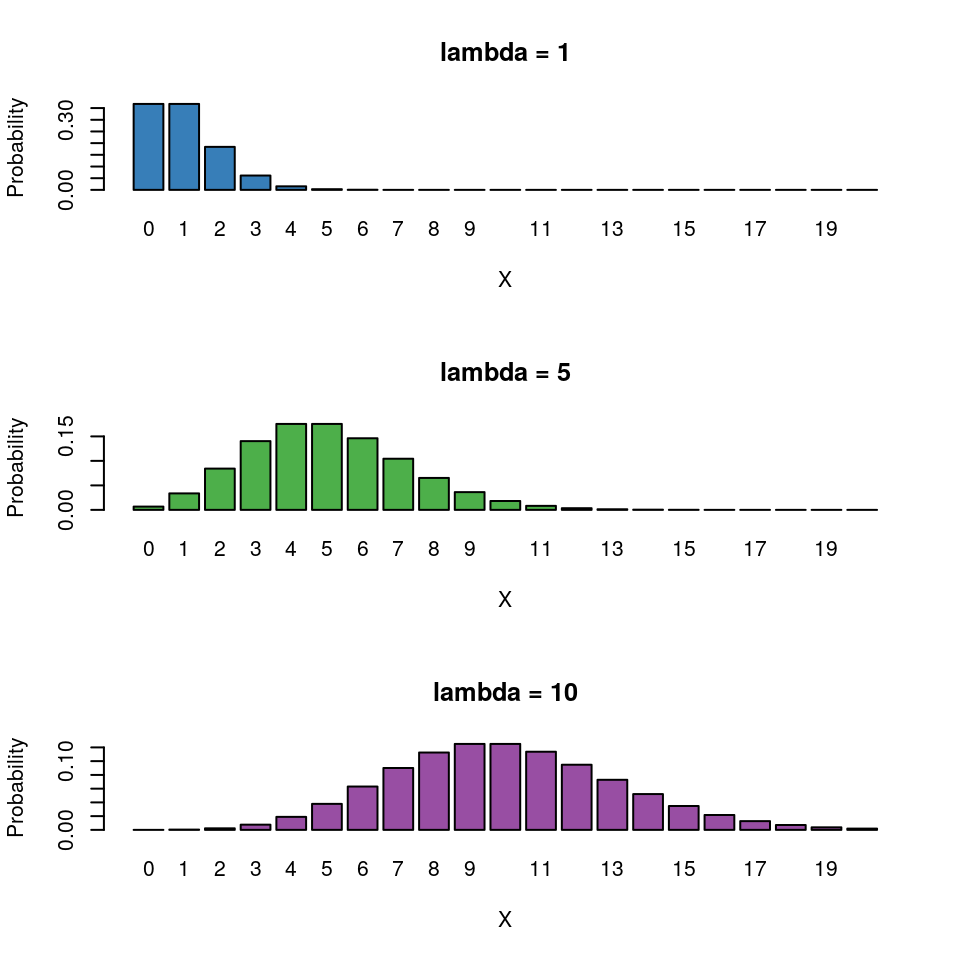
\includegraphics{_main_files/figure-latex/unnamed-chunk-79-1} \end{center}

So for the Poisson regression case we assume that the mean and variance
are the same. Hence, as the mean \emph{increases}, the variance
\emph{increases} also (\textbf{heteroscedascity}). This may or may not
be a sensible assumption so watch out!\footnote{the negative binomial
  model and others can cope with cases where this assumption is not
  satisfied}

Recall the link function and the rules of logarithms (if
\(\log{\lambda} = k\), then \(\lambda = e^k\)):

\[
\begin{aligned}
\log{\lambda} & = \beta_0 + \beta_1X \\
\lambda & = e^{\beta_0 + \beta_1X }
\end{aligned}
\] Thus we are effectively modelling the observed counts (on the
original scale) using an exponential mean function.

\begin{center}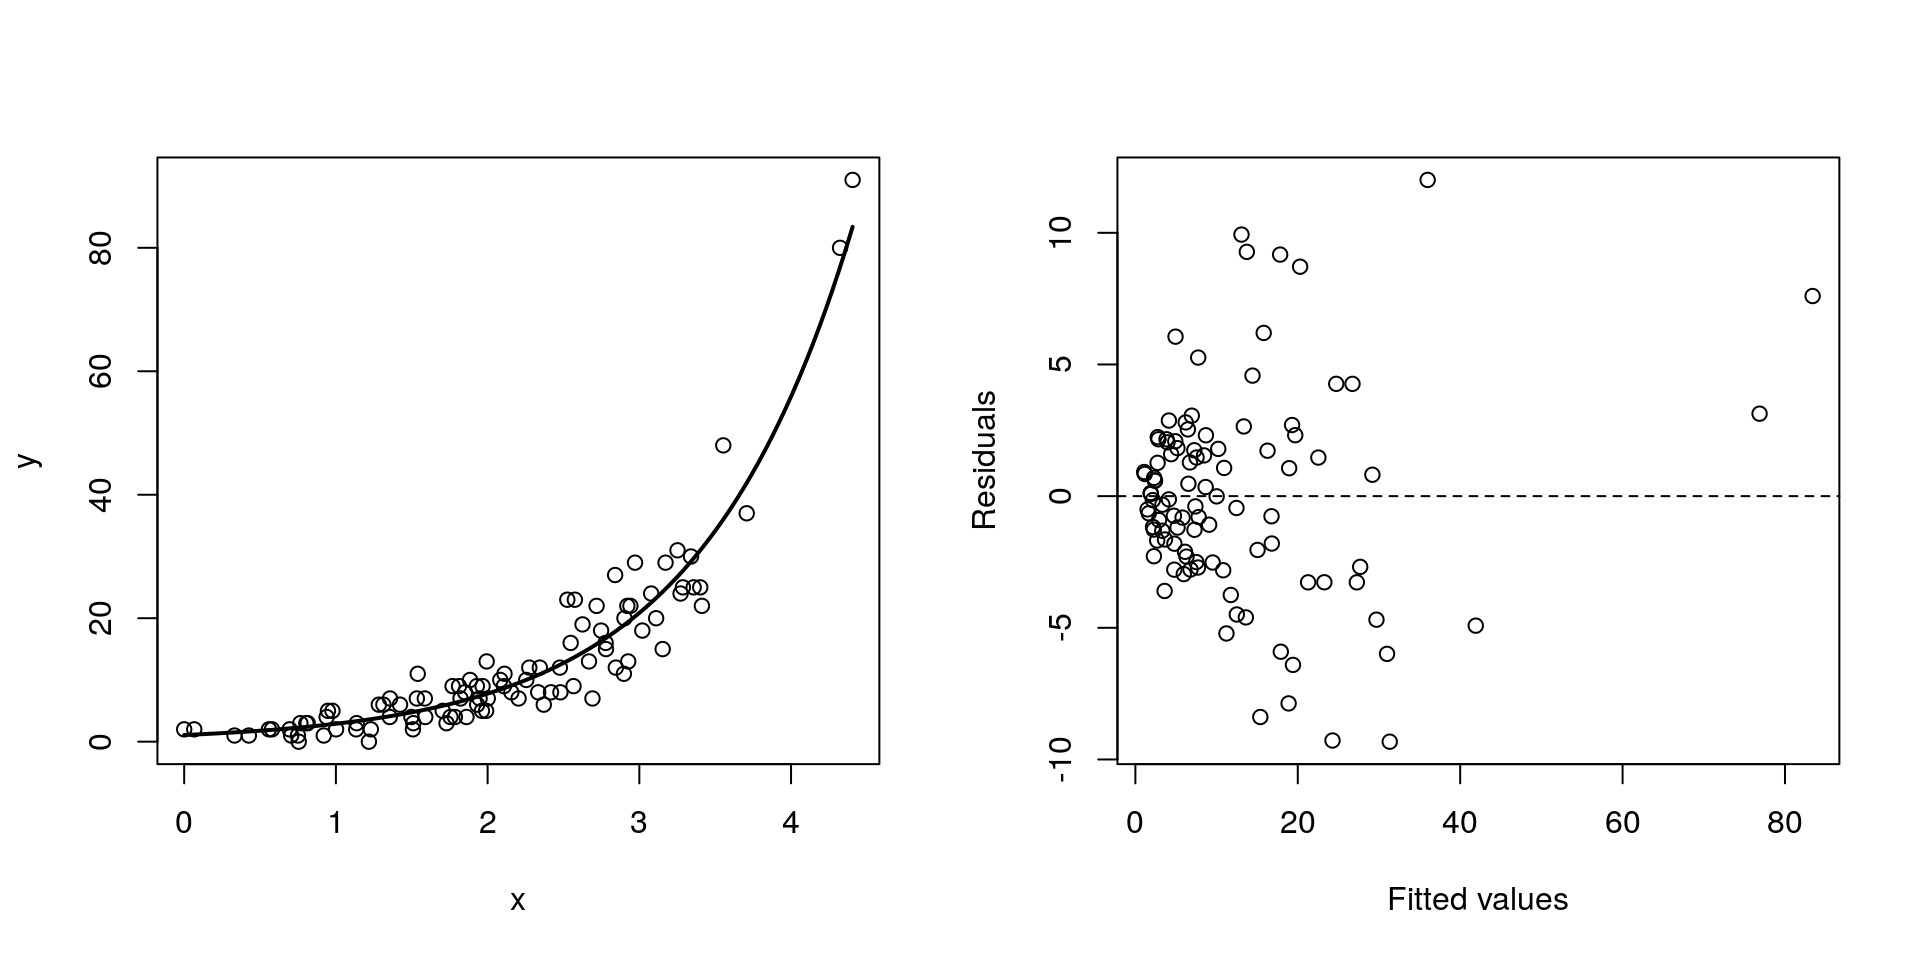
\includegraphics{_main_files/figure-latex/unnamed-chunk-80-1} \end{center}

\section{Example: Cuckoos}\label{example-cuckoos}

\begin{center}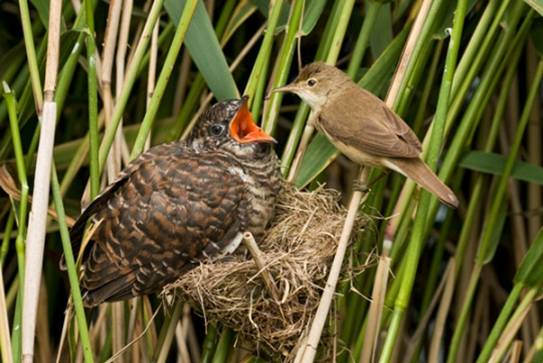
\includegraphics[width=0.75\linewidth]{_img/03-cuckoo} \end{center}

In a study by
\href{http://www.nature.com/nature/journal/v397/n6721/abs/397667a0.html}{Kilner
\emph{et al.} (1999)}, the authors studied the begging rate of nestlings
in relation to total mass of the brood of \textbf{reed warbler chicks}
and \textbf{cuckoo chicks}. The question of interest is:

\begin{quote}
How does nestling mass affect begging rates between the different
species?
\end{quote}

Download the data file from
\href{https://exeter-data-analytics.github.io/StatModelling/_data/cuckoo.csv}{here}
and save it to your working directory.\footnote{this dataset was
  obtained by digitising the plot that appear in the original paper,
  hence you will not be able to fully reproduce the results of the
  original paper, it is only used here for illustrative purposes}

\begin{Shaded}
\begin{Highlighting}[]
\NormalTok{cuckoo <-}\StringTok{ }\KeywordTok{read.csv}\NormalTok{(}\StringTok{"cuckoo.csv"}\NormalTok{, }\DataTypeTok{header=}\NormalTok{T)}
\end{Highlighting}
\end{Shaded}

\begin{Shaded}
\begin{Highlighting}[]
\KeywordTok{head}\NormalTok{(cuckoo)}
\end{Highlighting}
\end{Shaded}

\begin{verbatim}
##        Mass Beg Species
## 1  9.637522   0  Cuckoo
## 2 10.229151   0  Cuckoo
## 3 13.103706   0  Cuckoo
## 4 15.217391   0  Cuckoo
## 5 16.231884   0  Cuckoo
## 6 20.120773   0  Cuckoo
\end{verbatim}

The data columns are:

\begin{itemize}
\tightlist
\item
  \textbf{Mass}: nestling mass of chick in grams
\item
  \textbf{Beg}: begging calls per 6 secs
\item
  \textbf{Species}: Warbler or Cuckoo
\end{itemize}

\begin{Shaded}
\begin{Highlighting}[]
\KeywordTok{ggplot}\NormalTok{(cuckoo, }\KeywordTok{aes}\NormalTok{(}\DataTypeTok{x=}\NormalTok{Mass, }\DataTypeTok{y=}\NormalTok{Beg, }\DataTypeTok{colour=}\NormalTok{Species)) }\OperatorTok{+}\StringTok{ }\KeywordTok{geom_point}\NormalTok{()}
\end{Highlighting}
\end{Shaded}

\begin{center}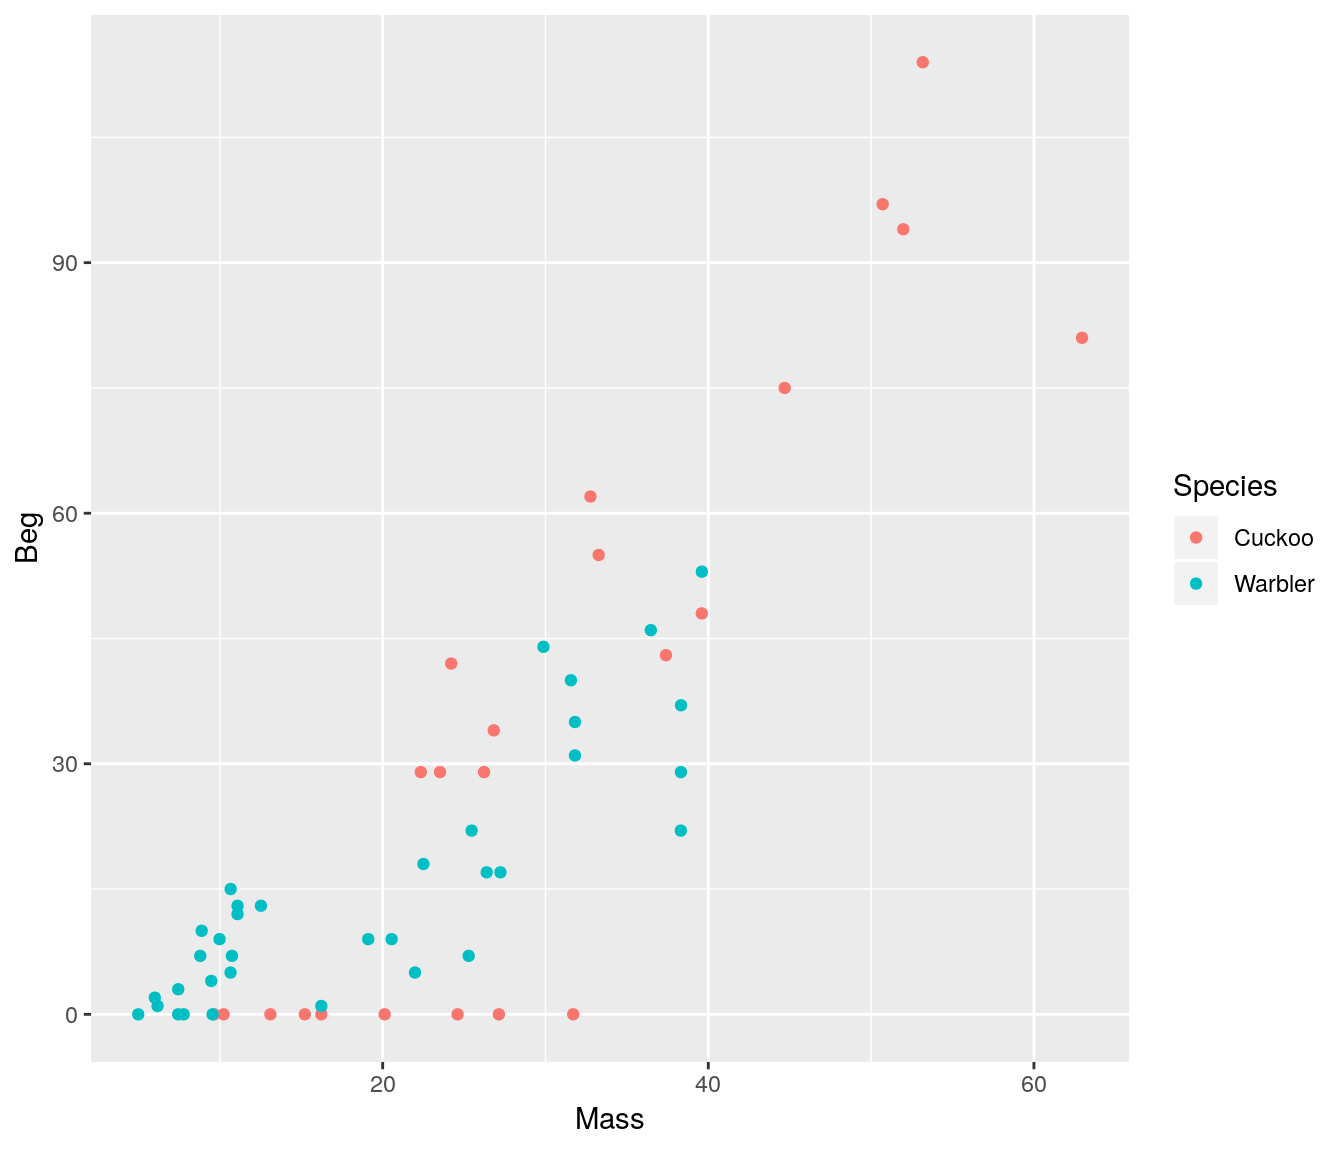
\includegraphics{_main_files/figure-latex/unnamed-chunk-85-1} \end{center}

There seem to be a relationship between mass and begging calls and it
could be different between species. It is tempting to fit a linear model
to this data. In fact, this is what the authors of the original paper
did; \textbf{reed warbler chicks} (solid circles, dashed fitted line)
and \textbf{cuckoo chick} (open circles, solid fitted line):

\begin{center}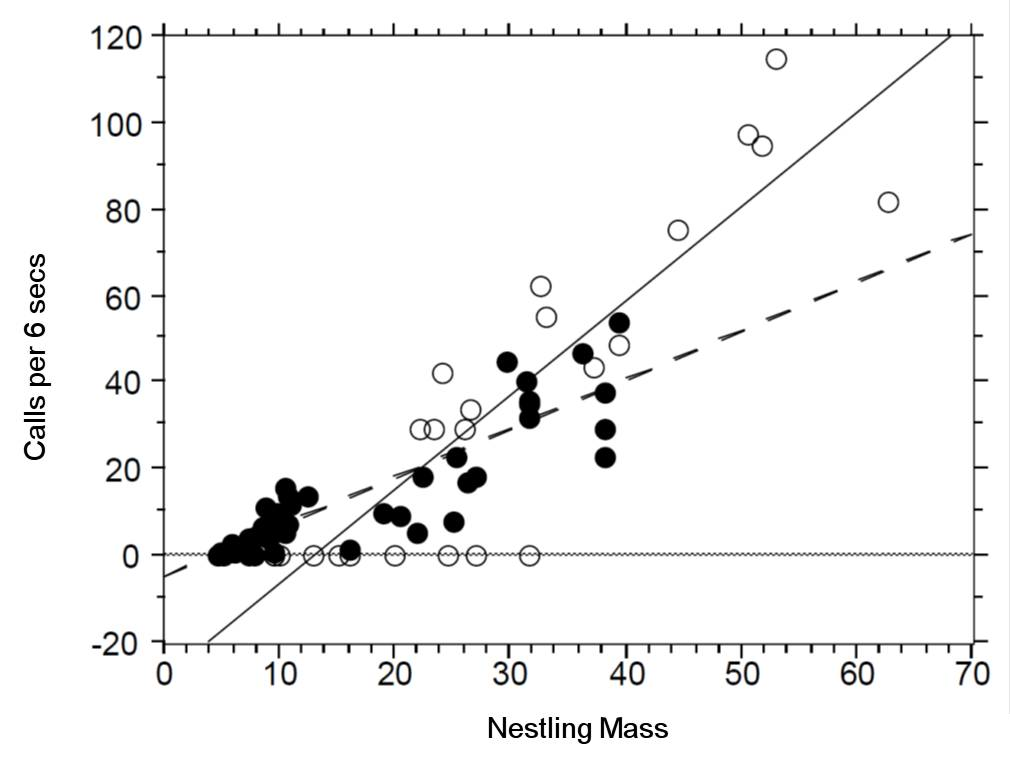
\includegraphics[width=0.75\linewidth]{_img/03-cuckooanalysis} \end{center}

This model is inadequate. It is predicting \textbf{negative} begging
calls \emph{within} the range of the observed data, which clearly does
not make any sense.

Let us display the model diagnostics plots for this linear model.

\begin{Shaded}
\begin{Highlighting}[]
\NormalTok{## Fit model}
\NormalTok{## We add an interaction term here, we will talk about this later on}
\NormalTok{fit <-}\StringTok{ }\KeywordTok{lm}\NormalTok{(Beg }\OperatorTok{~}\StringTok{ }\NormalTok{Mass}\OperatorTok{*}\NormalTok{Species, }\DataTypeTok{data=}\NormalTok{cuckoo) }
\end{Highlighting}
\end{Shaded}

\begin{Shaded}
\begin{Highlighting}[]
\KeywordTok{par}\NormalTok{(}\DataTypeTok{mfrow=}\KeywordTok{c}\NormalTok{(}\DecValTok{2}\NormalTok{, }\DecValTok{2}\NormalTok{))}
\KeywordTok{plot}\NormalTok{(fit, }\DataTypeTok{pch=}\DecValTok{19}\NormalTok{, }\DataTypeTok{col=}\StringTok{'darkgrey'}\NormalTok{)}
\end{Highlighting}
\end{Shaded}

\begin{center}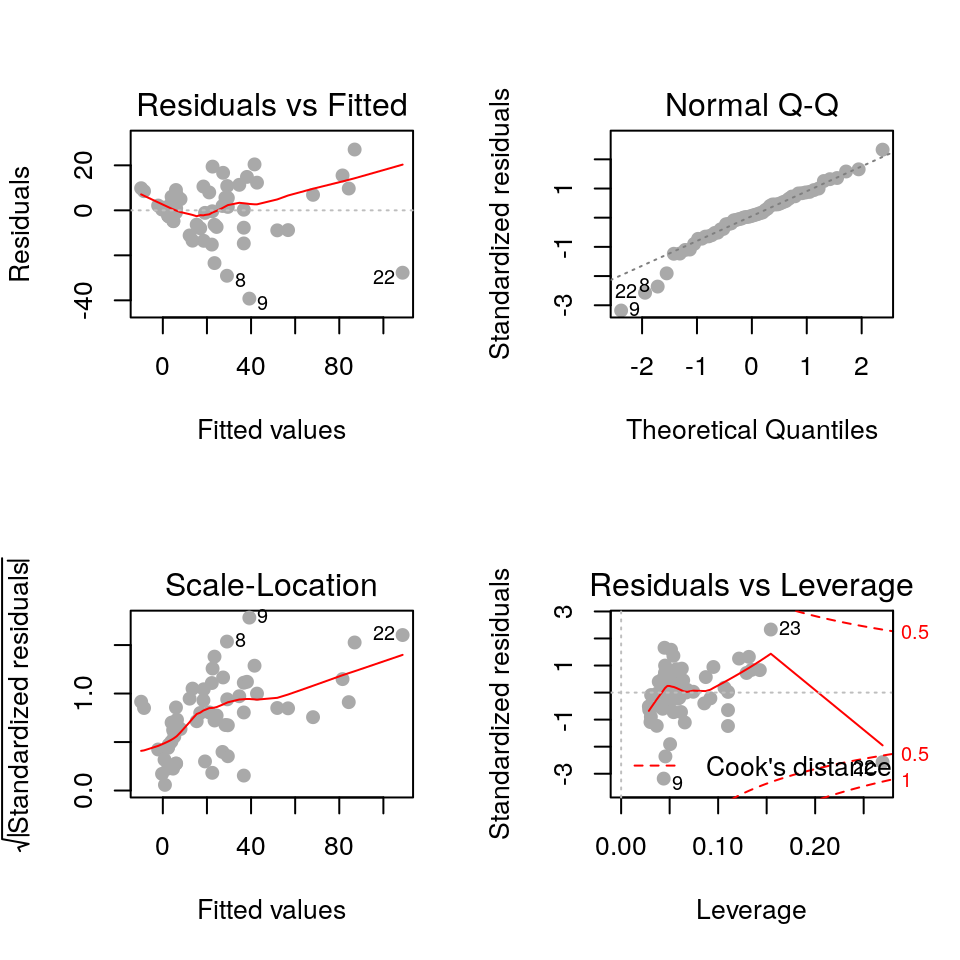
\includegraphics{_main_files/figure-latex/unnamed-chunk-88-1} \end{center}

The residuals plot depicts a ``funnelling'' effect, highlighting that
the model assumptions are violated. We should therefore try a different
model structure.

The response variable in this case is a classic \textbf{count data}:
\textbf{discrete} and bounded below by zero (i.e we cannot have negative
counts). We will therefore try a \textbf{Poisson model} using a
\textbf{log} link function for the mean:

\[
    \log{\lambda} = \beta_0 + \beta_1 M_i + \beta_2 S_i + \beta_3 M_i S_i
\]

where \(M_i\) is nestling mass and \(S_i\) a \textbf{dummy} variable
(refer to \protect\hyperlink{sec:categorical}{Categorical explanatory
variables}):

\[
S_i = \left\{\begin{array}{ll}
        1 & \mbox{if $i$ is warbler},\\
        0 & \mbox{otherwise}.
        \end{array}
        \right.
\]

The term \(M_iS_i\) is an \textbf{interaction} term. Think of this as an
additional explanatory variable in our model. Effectively it lets us
have \textbf{different} slopes for different species (without an
interaction term we assume that both species have the same slope for the
relationship between begging rate and mass, and only the intercept
differ).

The mean regression lines for the two species look like this:

\begin{itemize}
\tightlist
\item
  \textbf{Cuckoo} (\(S_i=0\))
\end{itemize}

\[
\begin{aligned}
    \log{\lambda} & = \beta_0 + \beta_1 M_i + (\beta_2 \times 0)  + (\beta_3 \times M_i \times 0)\\
    \log{\lambda} & = \beta_0 + \beta_1 M_i
\end{aligned}
\]

\begin{itemize}
\item
  \textbf{Intercept} = \(\beta_0\), \textbf{Gradient} = \(\beta_1\)
\item
  \textbf{Warbler} (\(S_i=1\))
\end{itemize}

\[
\begin{aligned}
    \log{\lambda} & = \beta_0 + \beta_1 M_i + (\beta_2 \times 1)  + (\beta_3 \times M_i \times 1)\\
    \log{\lambda} & = \beta_0 + \beta_1 M_i + \beta_2 + \beta_3M_i\\
    \log{\lambda} & = (\beta_0+\beta_2) + (\beta_1+\beta_3) M_i
\end{aligned}
\]

\begin{itemize}
\tightlist
\item
  \textbf{Intercept} = \(\beta_0 + \beta_2\), \textbf{Gradient} =
  \(\beta_1 + \beta_3\)
\end{itemize}

To specify an interaction term in R we use the
\href{https://www.rdocumentation.org/packages/stats/versions/3.5.1/topics/formula}{\texttt{*}}
operator.

\begin{itemize}
\tightlist
\item
  Model with \textbf{no} interaction term:
  \(\log{\lambda} = \beta_0 + \beta_1 M_i + \beta_2 S_i\)
\end{itemize}

\begin{Shaded}
\begin{Highlighting}[]
\KeywordTok{glm}\NormalTok{(Beg }\OperatorTok{~}\StringTok{ }\NormalTok{Mass }\OperatorTok{+}\StringTok{ }\NormalTok{Species, }\DataTypeTok{data=}\NormalTok{cuckoo, }\DataTypeTok{family=}\KeywordTok{poisson}\NormalTok{(}\DataTypeTok{link=}\NormalTok{log))}
\end{Highlighting}
\end{Shaded}

\begin{itemize}
\tightlist
\item
  Model \textbf{with} interaction term:
  \(\log{\lambda} = \beta_0 + \beta_1 M_i + \beta_2 S_i + \beta_3 M_i S_i\)
\end{itemize}

\begin{Shaded}
\begin{Highlighting}[]
\KeywordTok{glm}\NormalTok{(Beg }\OperatorTok{~}\StringTok{ }\NormalTok{Mass}\OperatorTok{*}\NormalTok{Species, }\DataTypeTok{data=}\NormalTok{cuckoo, }\DataTypeTok{family=}\KeywordTok{poisson}\NormalTok{(}\DataTypeTok{link=}\NormalTok{log))}
\end{Highlighting}
\end{Shaded}

Fit the model with the interaction term in R:

\begin{Shaded}
\begin{Highlighting}[]
\NormalTok{fit <-}\StringTok{ }\KeywordTok{glm}\NormalTok{(Beg }\OperatorTok{~}\StringTok{ }\NormalTok{Mass}\OperatorTok{*}\NormalTok{Species, }\DataTypeTok{data=}\NormalTok{cuckoo, }\DataTypeTok{family=}\KeywordTok{poisson}\NormalTok{(}\DataTypeTok{link=}\NormalTok{log))}
\KeywordTok{summary}\NormalTok{(fit)}
\end{Highlighting}
\end{Shaded}

\begin{verbatim}
## 
## Call:
## glm(formula = Beg ~ Mass * Species, family = poisson(link = log), 
##     data = cuckoo)
## 
## Deviance Residuals: 
##     Min       1Q   Median       3Q      Max  
## -7.4570  -3.0504  -0.0006   1.9389   5.2139  
## 
## Coefficients:
##                      Estimate Std. Error z value Pr(>|z|)    
## (Intercept)          1.589861   0.104531  15.209  < 2e-16 ***
## Mass                 0.054736   0.002298  23.820  < 2e-16 ***
## SpeciesWarbler      -0.535546   0.161304  -3.320 0.000900 ***
## Mass:SpeciesWarbler  0.015822   0.004662   3.394 0.000689 ***
## ---
## Signif. codes:  0 '***' 0.001 '**' 0.01 '*' 0.05 '.' 0.1 ' ' 1
## 
## (Dispersion parameter for poisson family taken to be 1)
## 
##     Null deviance: 1730.04  on 57  degrees of freedom
## Residual deviance:  562.08  on 54  degrees of freedom
## AIC: 784.81
## 
## Number of Fisher Scoring iterations: 5
\end{verbatim}

For the sake of clarity here is the mapping of the \(\beta_p\)
regression coefficients used above and those returned by R.

\begin{itemize}
\tightlist
\item
  \texttt{(Intercept)} = \(\beta_0\) (intercept for the
  \textbf{reference/baseline} species, \textbf{cuckoo} in this case)
\item
  \texttt{Mass} = \(\beta_1\) (slope for the baseline species)
\item
  \texttt{SpeciesWarbler} = \(\beta_2\) (the increase/decrease in
  intercept relative to the baseline species)
\item
  \texttt{Mass:SpeciesWarbler} = \(\beta_3\) (the increase/decrease in
  slope relative to the baseline species)
\end{itemize}

Plot the mean regression line for each species:

\begin{Shaded}
\begin{Highlighting}[]
\NormalTok{newdata <-}\StringTok{ }\KeywordTok{expand.grid}\NormalTok{(}\DataTypeTok{Mass=}\KeywordTok{seq}\NormalTok{(}\KeywordTok{min}\NormalTok{(cuckoo}\OperatorTok{$}\NormalTok{Mass), }\KeywordTok{max}\NormalTok{(cuckoo}\OperatorTok{$}\NormalTok{Mass), }\DataTypeTok{length.out=}\DecValTok{200}\NormalTok{),}
                       \DataTypeTok{Species=}\KeywordTok{levels}\NormalTok{(cuckoo}\OperatorTok{$}\NormalTok{Species))}
\NormalTok{newdata <-}\StringTok{ }\KeywordTok{cbind}\NormalTok{(newdata, }\DataTypeTok{Beg=}\KeywordTok{predict}\NormalTok{(fit, newdata, }\DataTypeTok{type=}\StringTok{'response'}\NormalTok{))}


\KeywordTok{ggplot}\NormalTok{(}\DataTypeTok{mapping=}\KeywordTok{aes}\NormalTok{(}\DataTypeTok{x=}\NormalTok{Mass, }\DataTypeTok{y=}\NormalTok{Beg, }\DataTypeTok{colour=}\NormalTok{Species)) }\OperatorTok{+}\StringTok{ }\KeywordTok{geom_point}\NormalTok{(}\DataTypeTok{data=}\NormalTok{cuckoo) }\OperatorTok{+}\StringTok{ }
\StringTok{    }\KeywordTok{geom_line}\NormalTok{(}\DataTypeTok{data=}\NormalTok{newdata)}
\end{Highlighting}
\end{Shaded}

\begin{center}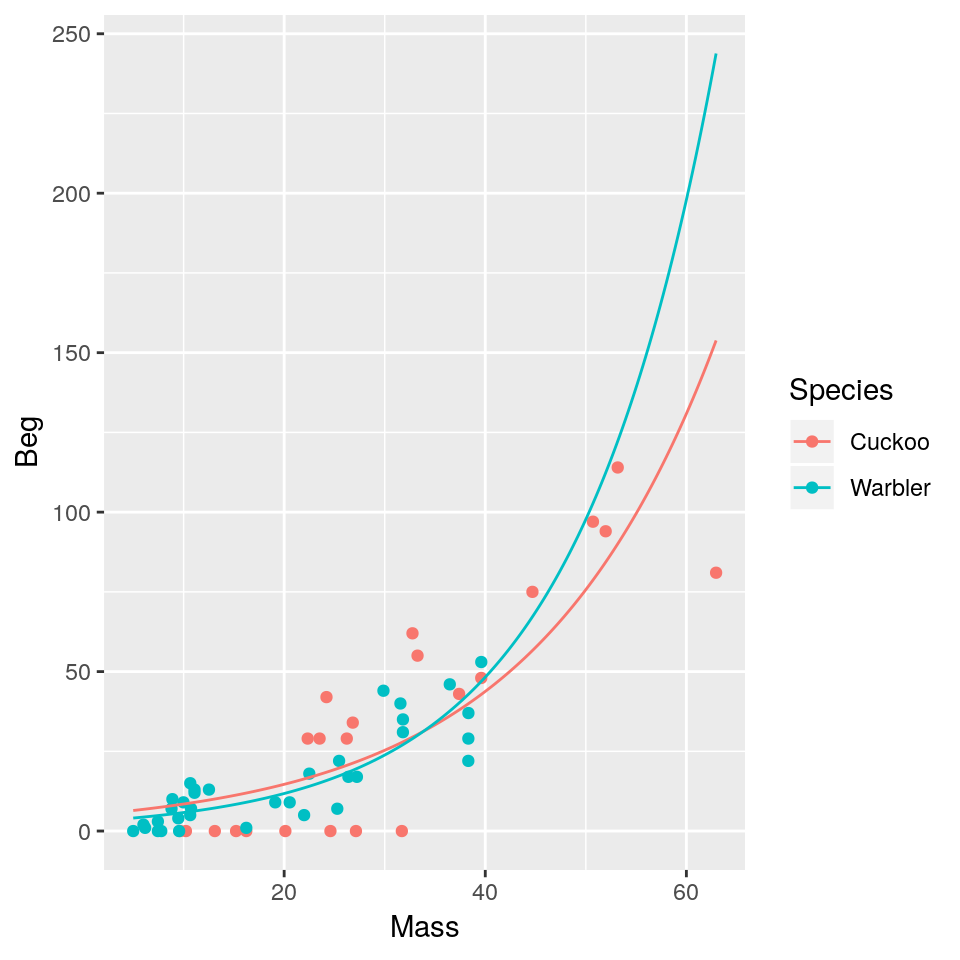
\includegraphics{_main_files/figure-latex/unnamed-chunk-92-1} \end{center}

We get an exponential curve in the scale of the original data, which is
the \textbf{same} as a straight line in the log-scaled version of the
data.

\section{Practical 4 - Species
richness}\label{practical-4---species-richness}

A long-term agricultural experiment had 90 grassland plots, each 25m x
25m, differing in biomass, soil pH and species richness (the count of
species in the whole plot). It is well known that species richness
declines with increasing biomass, but the question addressed here is
whether the slope of that relationship differs with soil pH (i.e there's
an interaction effect). The plots were classified according to a 3-level
factor as high, medium or low pH with 30 plots in each level.

The response variable is the \textbf{count} of species
(\texttt{Species}), so a GLM with Poisson errors is a sensible choice.
The continuous explanatory variable is long-term average biomass
measured in June (\texttt{Biomass}), and the categorical explanatory
variable is soil pH (\texttt{pH}).

Download the data from
\href{https://exeter-data-analytics.github.io/StatModelling/_data/species.csv}{here}

\begin{Shaded}
\begin{Highlighting}[]
\NormalTok{df <-}\StringTok{ }\KeywordTok{read.csv}\NormalTok{(}\StringTok{"species.csv"}\NormalTok{, }\DataTypeTok{header=}\NormalTok{T)}
\end{Highlighting}
\end{Shaded}

\begin{Shaded}
\begin{Highlighting}[]
\KeywordTok{head}\NormalTok{(df)}
\end{Highlighting}
\end{Shaded}

\begin{verbatim}
##     pH   Biomass Species
## 1 high 0.4692972      30
## 2 high 1.7308704      39
## 3 high 2.0897785      44
## 4 high 3.9257871      35
## 5 high 4.3667927      25
## 6 high 5.4819747      29
\end{verbatim}

\begin{Shaded}
\begin{Highlighting}[]
\KeywordTok{ggplot}\NormalTok{(df, }\KeywordTok{aes}\NormalTok{(}\DataTypeTok{x=}\NormalTok{Biomass, }\DataTypeTok{y=}\NormalTok{Species, }\DataTypeTok{colour=}\NormalTok{pH)) }\OperatorTok{+}\StringTok{ }\KeywordTok{geom_point}\NormalTok{()}
\end{Highlighting}
\end{Shaded}

\begin{center}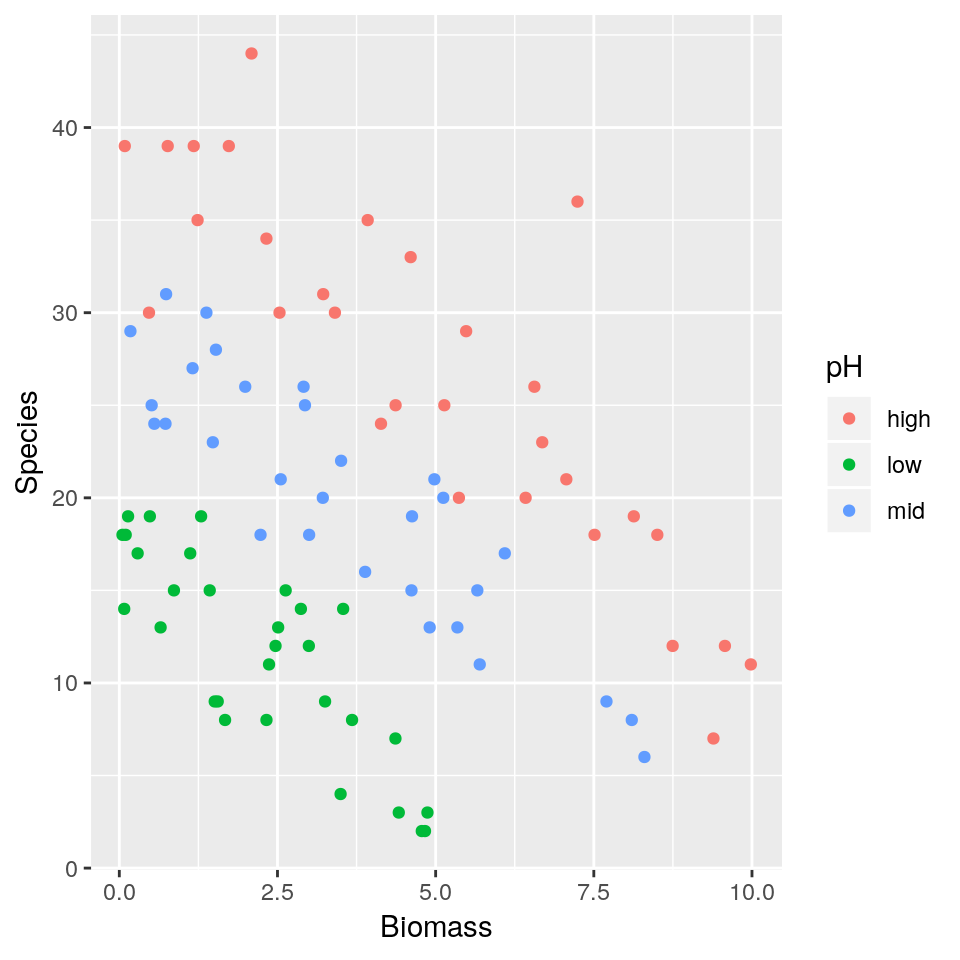
\includegraphics{_main_files/figure-latex/unnamed-chunk-96-1} \end{center}

\hypertarget{tsk11}{}\bblockT[Task]{\phantomsection\label{sol11}11}

\begin{enumerate}
\def\labelenumi{\arabic{enumi}.}
\tightlist
\item
  Fit a simple linear regression model (i.e assuming residuals to be
  normally distributed) with \texttt{Species} as response variable and
  \texttt{Biomass} and \texttt{pH} as explanatory variables. Assume a
  \textbf{different} slope for each \texttt{pH} level. Display a summary
  of the fit.
\item
  Plot the mean regression lines for all three \texttt{pH} levels (low,
  medium, high)
\item
  As \texttt{Biomass} tends to increase what is the expected number of
  species found in the grassland for the different pH levels? Is this
  biologically plausible?
\item
  Repeat 1--3 this time fitting a \textbf{Poisson} regression model.
\end{enumerate}

\eblockT

\hyperlink{sol11}{\buttonS{Show Solution on P\colpageref{tsk11}}}

\section{Logistic regression (for binary
data)}\label{logistic-regression-for-binary-data}

So far we have only considered continuous and discrete data as response
variables. What if our response is a categorical variable (e.g passing
or failing an exam, voting yes or no in a referendum, whether an egg has
successfully fledged or been predated)?

We can model the \textbf{probability} \(p\) of being in a particular
class as a function of other explanatory variables. Here we will focus
on variables with two levels (e.g dead/alive). \footnote{the multinomial
  logistic regression model generalises logistic regression to
  multiclass problems}. These type of \textbf{binary} data are assumed
to follow a \textbf{Bernoulli} distribution which has the following
characteristics:

\[
Y \sim \mathcal{Bern}(p)
\]

\begin{itemize}
\tightlist
\item
  \textbf{Binary} variable, taking the values 0 or 1 (yes/no,
  pass/fail).
\item
  A \textbf{probability} parameter \(p\), where \(0 < p < 1\).
\item
  \textbf{Mean} = \(p\)\\
\item
  \textbf{Variance} = \(p(1 - p)\)
\end{itemize}

\begin{center}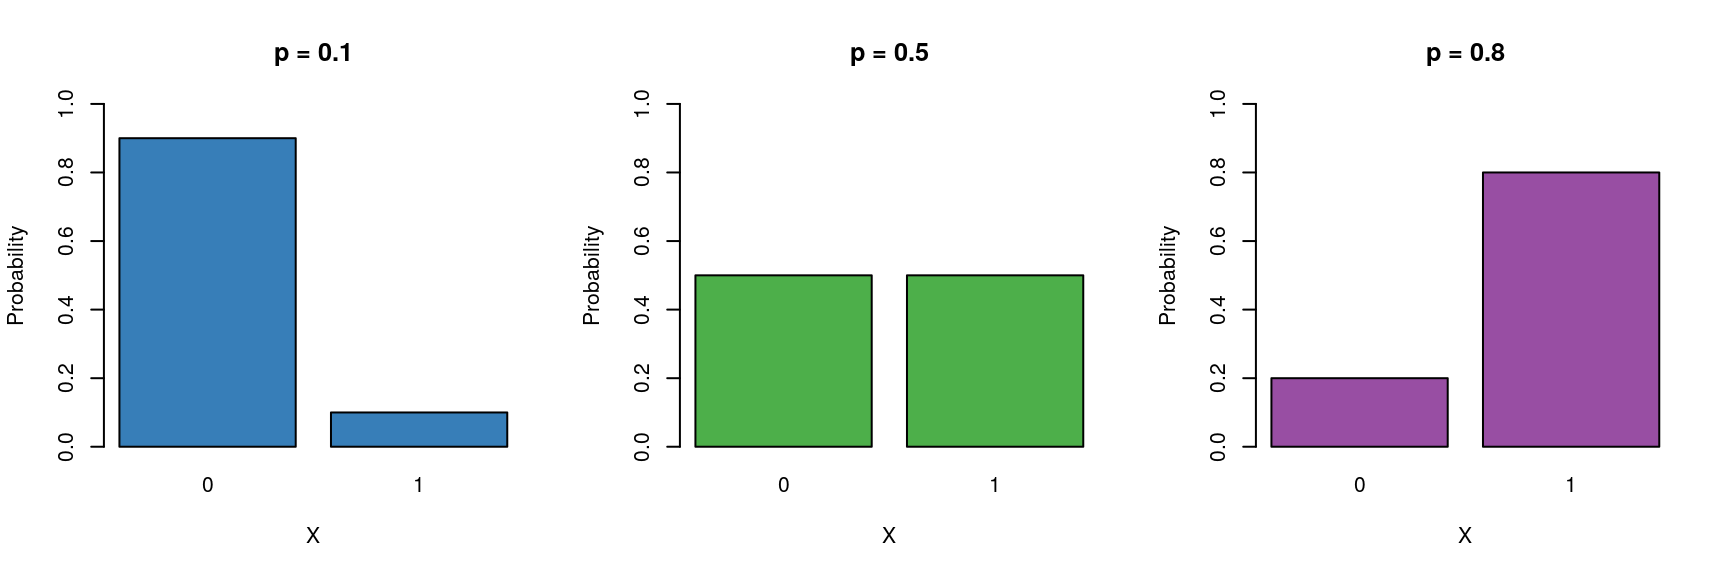
\includegraphics{_main_files/figure-latex/bernplot-1} \end{center}

Let us now place the Gaussian (simple linear regression), Poisson and
logistic models next to each other:

\[
\begin{aligned}
Y & \sim \mathcal{N}(\mu, \sigma^2) &&& Y  \sim \mathcal{Pois}(\lambda) &&& Y  \sim \mathcal{Bern}(p)\\
\mu & = \beta_0 + \beta_1X &&& \log{\lambda} = \beta_0 + \beta_1X &&& ?? = \beta_0 + \beta_1X
\end{aligned}
\]

Now we need to fill in the \texttt{??} with the appropriate term.
Similar to the Poisson regression case, we cannot simply model the
probabiliy as \(p = \beta_0 + \beta_1X\), because \(p\) \textbf{cannot}
be negative. \(\log{p} = \beta_0 + \beta_1X\) won't work either, because
\(p\) cannot be greater than 1. Instead we model the \textbf{log odds}
\(\log\left(\frac{p}{1 - p}\right)\) as a linear function. So our
logistic regression model looks like this:

\[
\begin{aligned}
Y  & \sim \mathcal{Bern}(p)\\
\log\left(\frac{p}{1 - p}\right) &  = \beta_0 + \beta_1 X
\end{aligned}
\]

Again, note that we are still ``only'' fitting straight lines through
our data, but this time in the log odds space. As a shorthand notation
we write
\(\log\left(\frac{p}{1 - p}\right) = \text{logit}(p) = \beta_0 + \beta_1 X\).

\begin{center}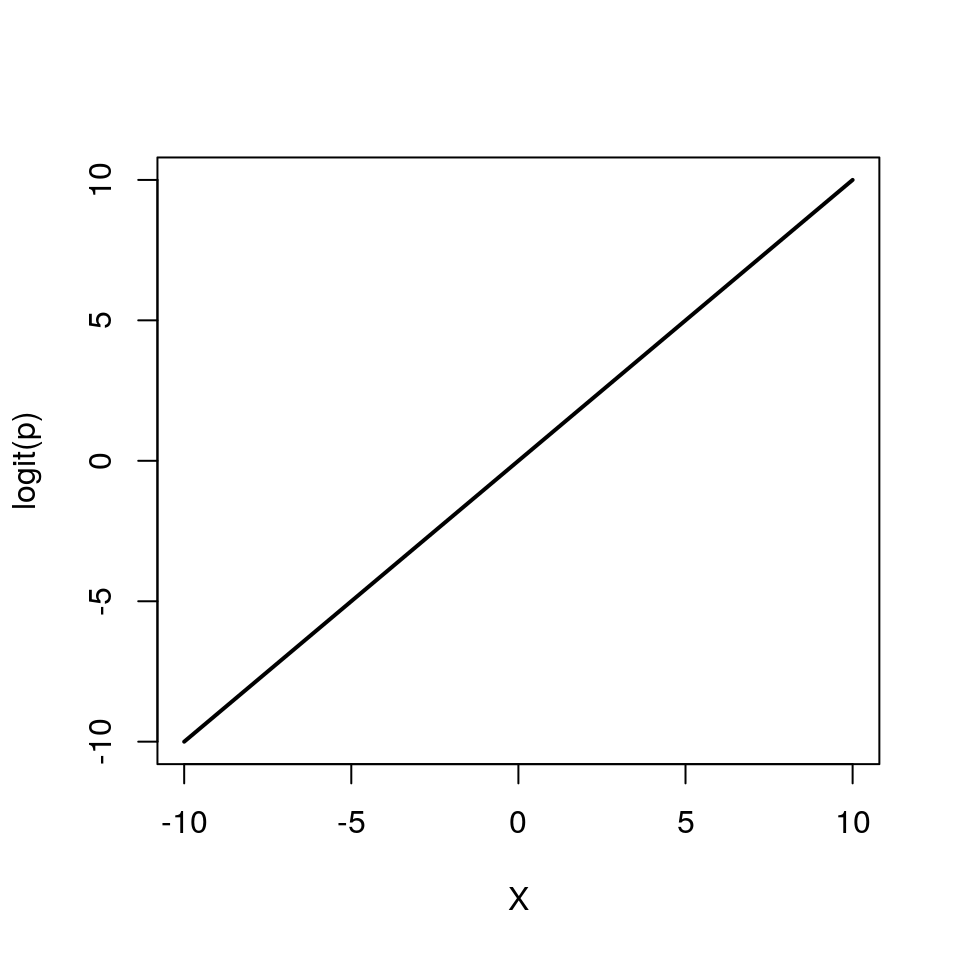
\includegraphics{_main_files/figure-latex/unnamed-chunk-99-1} \end{center}

We can also re-arrange the above equation so that we get an expression
for \(p\)

\[
p = \frac{e^{\beta_0 + \beta_1 X}}{1 + e^{\beta_0 + \beta_1 X}}
\]

\begin{center}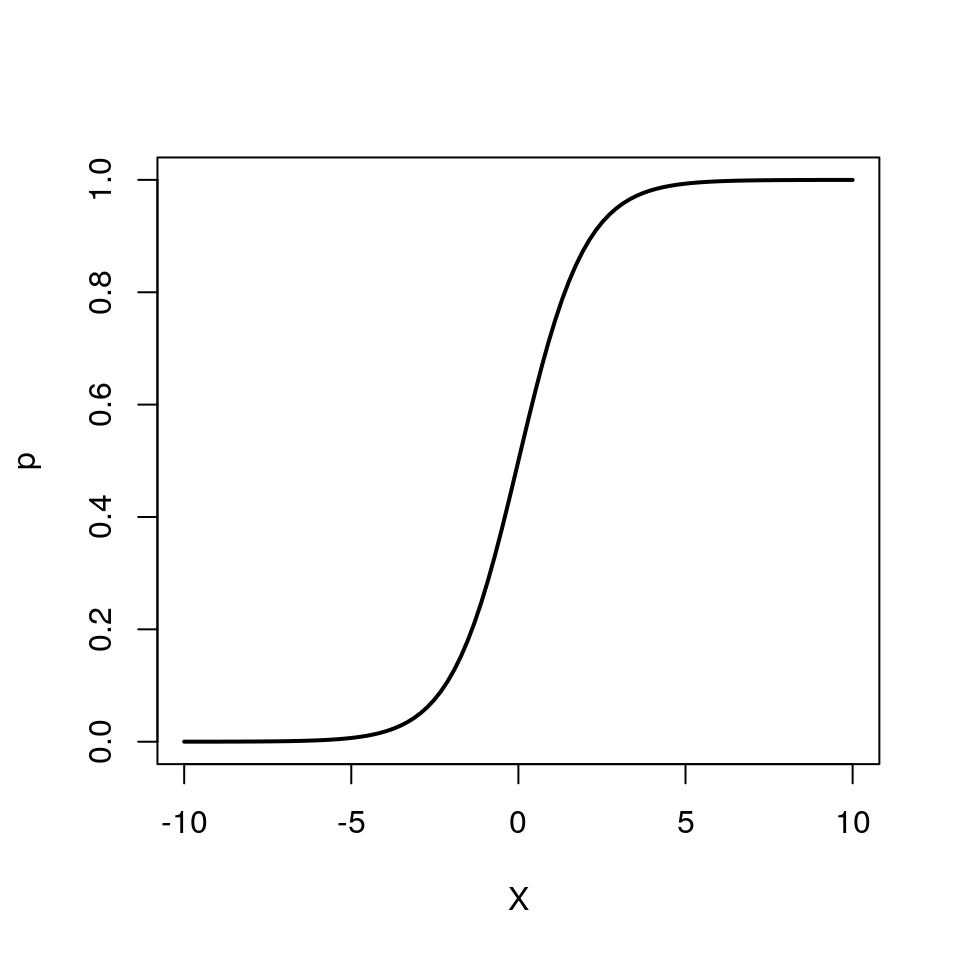
\includegraphics{_main_files/figure-latex/unnamed-chunk-100-1} \end{center}

Note how \(p\) can only vary between 0 and 1.

To implement the logistic regression model in R, we choose
\texttt{family=binomial(link=logit)} (the Bernoulli distribution is a
special case of the Binomial distribution when the number of trials is
1).

\begin{Shaded}
\begin{Highlighting}[]
\KeywordTok{glm}\NormalTok{(response }\OperatorTok{~}\StringTok{ }\NormalTok{explanatory, }\DataTypeTok{family=}\KeywordTok{binomial}\NormalTok{(}\DataTypeTok{link=}\NormalTok{logit))}
\end{Highlighting}
\end{Shaded}

\section{Example: 1992 US election
survey}\label{example-1992-us-election-survey}

Voters were asked if they preferred George Bush (Republican) or Bill
Clinton (Democrat) (voters who preferred other candidates were
excluded). The respondent's income was characterised on a 5-point scale
(1 - poor to 5 - rich). The question of interest in this case is:

\begin{quote}
Do voters with higher incomes prefer conservative\footnote{i.e.~Republican}
candidates?
\end{quote}

Download the data file from
\href{https://exeter-data-analytics.github.io/StatModelling/_data/US1992.csv}{here}
and save it to your working directory.

\begin{Shaded}
\begin{Highlighting}[]
\NormalTok{USA <-}\StringTok{ }\KeywordTok{read.csv}\NormalTok{(}\StringTok{"US1992.csv"}\NormalTok{, }\DataTypeTok{header=}\NormalTok{T)}
\end{Highlighting}
\end{Shaded}

\begin{Shaded}
\begin{Highlighting}[]
\KeywordTok{head}\NormalTok{(USA)}
\end{Highlighting}
\end{Shaded}

\begin{verbatim}
##           Vote Income
## 1  George Bush      4
## 2  George Bush      2
## 3 Bill Clinton      1
## 4  George Bush      2
## 5 Bill Clinton      3
## 6 Bill Clinton      4
\end{verbatim}

The data columns are:

\begin{itemize}
\tightlist
\item
  \textbf{Vote}: Whether voter preferred Bill Clinton (Democrat) or
  George Bush (Republican)
\item
  \textbf{Income}: 1 - poor to 5 - rich (based on quantiles of earnings
  in the US)
\end{itemize}

\begin{Shaded}
\begin{Highlighting}[]
\KeywordTok{ggplot}\NormalTok{(USA, }\KeywordTok{aes}\NormalTok{(}\DataTypeTok{x=}\NormalTok{Income)) }\OperatorTok{+}\StringTok{ }\KeywordTok{geom_bar}\NormalTok{(}\KeywordTok{aes}\NormalTok{(}\DataTypeTok{fill=}\NormalTok{Vote))}
\end{Highlighting}
\end{Shaded}

\begin{center}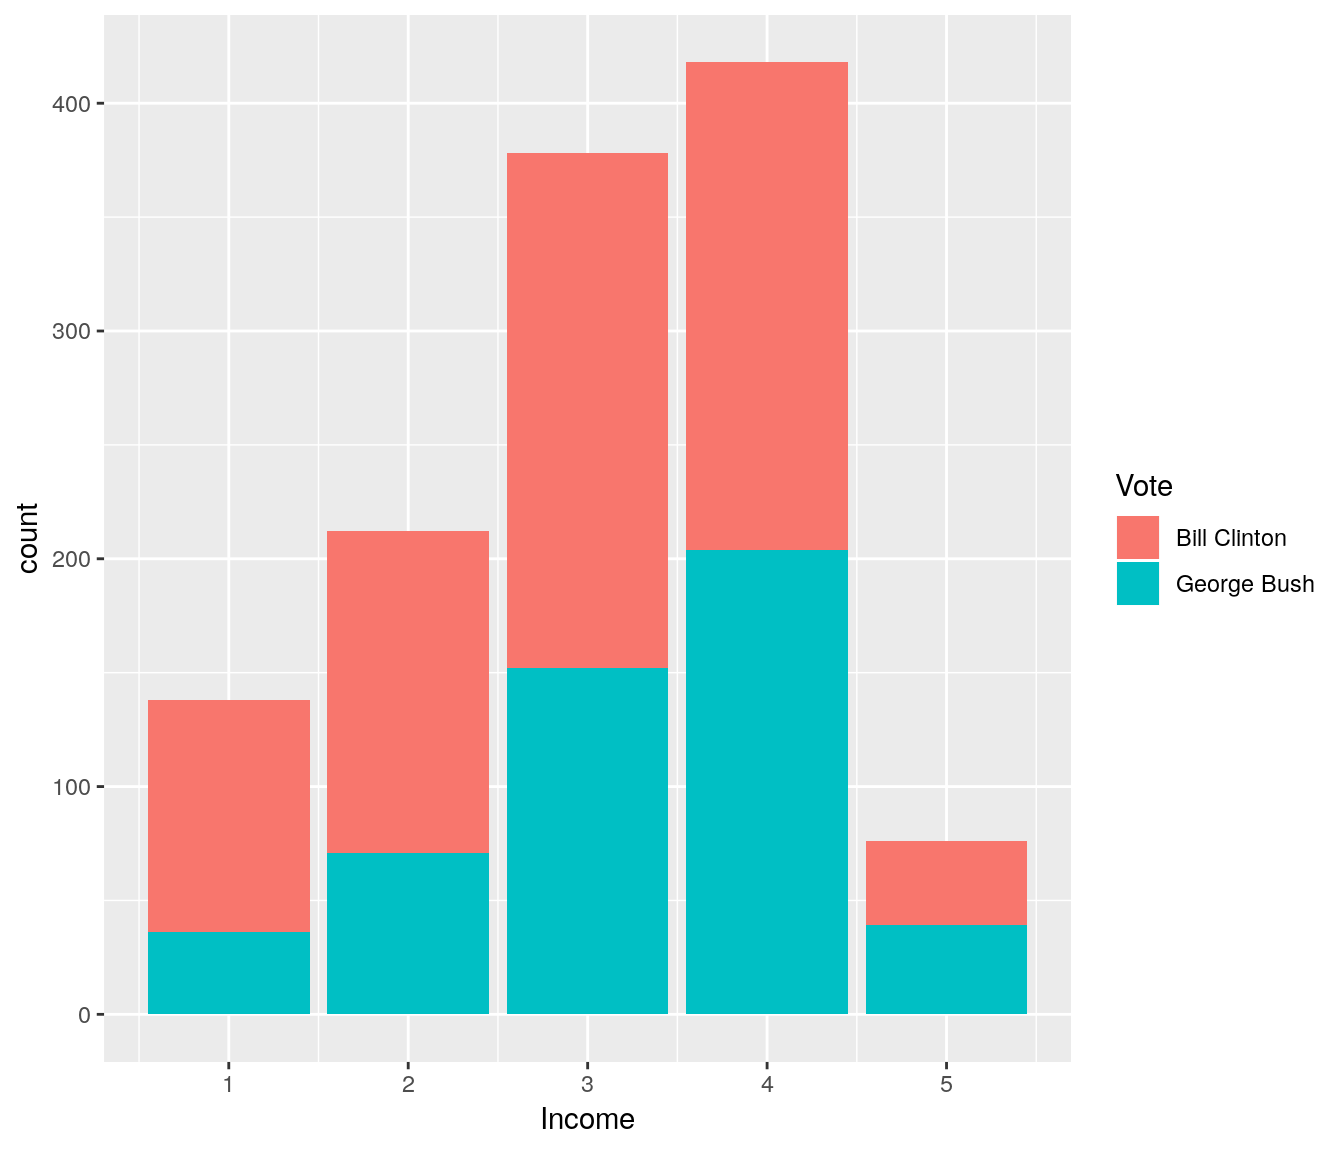
\includegraphics{_main_files/figure-latex/unnamed-chunk-105-1} \end{center}

It does look like people with low income are more likely to prefer Bill
Clinton over George Bush. Let us fit a logistic regression model to dig
deeper into this. Note that by default R will use the order of the
levels to define which one is class ``0'' (fail) and which one is class
``1'' (success).

\begin{Shaded}
\begin{Highlighting}[]
\KeywordTok{levels}\NormalTok{(USA}\OperatorTok{$}\NormalTok{Vote) }\CommentTok{# class 0, class 1}
\end{Highlighting}
\end{Shaded}

\begin{verbatim}
## [1] "Bill Clinton" "George Bush"
\end{verbatim}

So in this case \(p\) will represent the probability of preferring
George Bush. The probability of preferring Bill Clinton is simply
\(1-p\) because we are only considering two options.

\begin{Shaded}
\begin{Highlighting}[]
\NormalTok{fit <-}\StringTok{ }\KeywordTok{glm}\NormalTok{(Vote }\OperatorTok{~}\StringTok{ }\NormalTok{Income, }\DataTypeTok{data=}\NormalTok{USA, }\DataTypeTok{family=}\KeywordTok{binomial}\NormalTok{(}\DataTypeTok{link=}\NormalTok{logit))}
\KeywordTok{summary}\NormalTok{(fit)}
\end{Highlighting}
\end{Shaded}

\begin{verbatim}
## 
## Call:
## glm(formula = Vote ~ Income, family = binomial(link = logit), 
##     data = USA)
## 
## Deviance Residuals: 
##     Min       1Q   Median       3Q      Max  
## -1.2699  -1.0162  -0.8998   1.2152   1.6199  
## 
## Coefficients:
##             Estimate Std. Error z value Pr(>|z|)    
## (Intercept)  -1.3017     0.1828  -7.122 1.06e-12 ***
## Income        0.3033     0.0551   5.505 3.69e-08 ***
## ---
## Signif. codes:  0 '***' 0.001 '**' 0.01 '*' 0.05 '.' 0.1 ' ' 1
## 
## (Dispersion parameter for binomial family taken to be 1)
## 
##     Null deviance: 1655.0  on 1221  degrees of freedom
## Residual deviance: 1623.5  on 1220  degrees of freedom
## AIC: 1627.5
## 
## Number of Fisher Scoring iterations: 4
\end{verbatim}

Recall that we are fitting the model:

\[
\begin{aligned}
Y  & \sim \mathcal{Bern}(p)\\
\log\left(\frac{p}{1 - p}\right) &  = \beta_0 + \beta_1 X
\end{aligned}
\]

\begin{itemize}
\tightlist
\item
  \texttt{(Intercept)} = \(\beta_0\) = -1.3
\item
  \texttt{Income} = \(\beta_1\) = 0.303
\end{itemize}

It is common to interpret variables according to some \textbf{central
tendency} e.g at the central income category (i.e X=3):

\[
\begin{aligned}
P(\mbox{Republican vote at}~X = 3) &= \mbox{logit}^{-1}\left(-1.3 + 0.3 \times 3\right)\\
&= \frac{e^{-1.3 + 0.3 \times 3}}{1 + e^{-1.3 + 0.3 \times 3}}\\
&= 0.4.
\end{aligned}
\] We can also check for \(X=4\) and \(X=5\) (rich)

\[
\begin{aligned}
P(\mbox{Republican vote at}~X = 4) &= \mbox{logit}^{-1}\left(-1.3 + 0.3 \times 4\right)\\
&= \frac{e^{-1.3 + 0.3 \times 4}}{1 + e^{-1.3 + 0.3 \times 4}}\\
&= 0.48.
\end{aligned}
\]

\[
\begin{aligned}
P(\mbox{Republican vote at}~X = 5) &= \mbox{logit}^{-1}\left(-1.3 + 0.3 \times 5\right)\\
&= \frac{e^{-1.3 + 0.3 \times 5}}{1 + e^{-1.3 + 0.3 \times 5}}\\
&= 0.55.
\end{aligned}
\]

So there is a tendency for voters with higher incomes to prefer
Republicans over Democrats.

An \textbf{increase} of 1 unit on the \textbf{income scale} results in a
positive difference of 0.3 on the \textbf{logit} scale in support of
Bush.

A convenient way to express this on the \textbf{probability scale} is to
consider what effect a 1 unit change has close to the \textbf{central
value}, e.g.~between \(X = 3\) and \(X = 2\)

\[
\begin{aligned}
& \mbox{logit}^{-1}\left(-1.3 + 0.3 \times 3\right) \\
&~~~~~~~~- \mbox{logit}^{-1}\left(-1.3 + 0.3 \times 2\right) = 0.07.
\end{aligned}
\]

Hence an increase in income of 1 unit around this central value results
in a 7\% increase in the probability of supporting Bush.

\subsection{\texorpdfstring{The `divide-by-four'
rule}{The divide-by-four rule}}\label{the-divide-by-four-rule}

A useful \emph{rule-of-thumb} can be given by the
\textbf{`divide-by-four'} rule.

That is, the \textbf{maximum difference} in \(P(Y = 1)\) (P(Republican
vote) in our example) corresponding to a \textbf{unit} difference in
\(X\) is given by \(\beta / 4\).

In this example, the \textbf{maximum difference} in P(Republican vote)
corresponding to a \textbf{unit} difference in income is given by
\(0.3 / 4 = 0.076\) (or a 7.6\% change).

\subsection{Odds ratios}\label{odds-ratios}

An common interpretation of logistic regression coefficients is in terms
of \textbf{odds ratios}.

\textbf{Odds}:

\[
    \frac{P(\mbox{event happens})}{P(\mbox{event does not happen})}
\]

\textbf{Probability} of a voter in income category 3 voting Republican
is

\[
    \begin{aligned}
    P(\mbox{Republican vote for}~X = 3) &= p_{X = 3}\\
    &= \mbox{logit}^{-1}\left(-1.3 + 0.3 \times 3\right)\\
    &= 0.4.
    \end{aligned}
\]

\textbf{Odds}: \[\frac{p_{X = 3}}{1 - p_{X = 3}}\]

Odds of a voter in income category 3 voting Republican is 0.4 / 0.6 =
0.67.

\textbf{Odds ratio}:

\[
    \frac{\mbox{odds in one group}}{\mbox{odds in another group}}
\]

e.g.~odds ratio for voters in income category 3 voting Republican
compared to voters in income category 2 is:

\[
    \frac{\mbox{odds of voting Republican when}~X = 3}{\mbox{odds of voting Republican when}~X = 2} = \frac{\frac{p_{X = 3}}{1 - p_{X = 3}}}{\frac{p_{X = 2}}{1 - p_{X = 2}}}.
\]

Take \textbf{logs}:

\[
    \begin{aligned}
    \log\left(\frac{\frac{p_{X = 3}}{1 - p_{X = 3}}}{\frac{p_{X = 2}}{1 - p_{X = 2}}}\right) &= \log\left(\frac{p_{X = 3}}{1 - p_{X = 3}}\right) - \log\left(\frac{p_{X = 2}}{1 - p_{X = 2}}\right)\\
    &= \beta_0 + \left(\beta_1 \cdot 3\right) - \beta_0 - \left(\beta_1 \cdot 2\right)\\
    &= \beta_1 (3 - 2)\\
    &= \beta_1
    \end{aligned}
\]

So \(\beta_1\) is the \textbf{log-odds ratio} for voting Republican per
unit increase in income, and \(e^{\beta_1}\) is the \textbf{odds ratio}.
This measure does \textbf{not} rely on the \textbf{level} of income

In this example the \textbf{odds ratio} is \(e^{0.3}\) = 1.35.

\begin{quote}
Hence the odds of voting Republican increase by a factor of 1.35 per
unit increase in income.
\end{quote}

\textbf{Odds ratios} are a tricky thing to understand, and many people
(including me) find them \textbf{unintuitive}.

Are useful in \textbf{case-control} studies, where the prevalence of an
outcome is unknown.

\subsection{Model diagnostics}\label{model-diagnostics}

Once we have fitted a regression model, we can use it to predict the
\textbf{mean} probability of success for given individual
(\textbf{fitted values}).

We can then generate \textbf{residual plots} as before:

\begin{Shaded}
\begin{Highlighting}[]
\KeywordTok{plot}\NormalTok{(fit, }\DataTypeTok{which =} \KeywordTok{c}\NormalTok{(}\DecValTok{1}\NormalTok{, }\DecValTok{5}\NormalTok{))}
\end{Highlighting}
\end{Shaded}

\begin{center}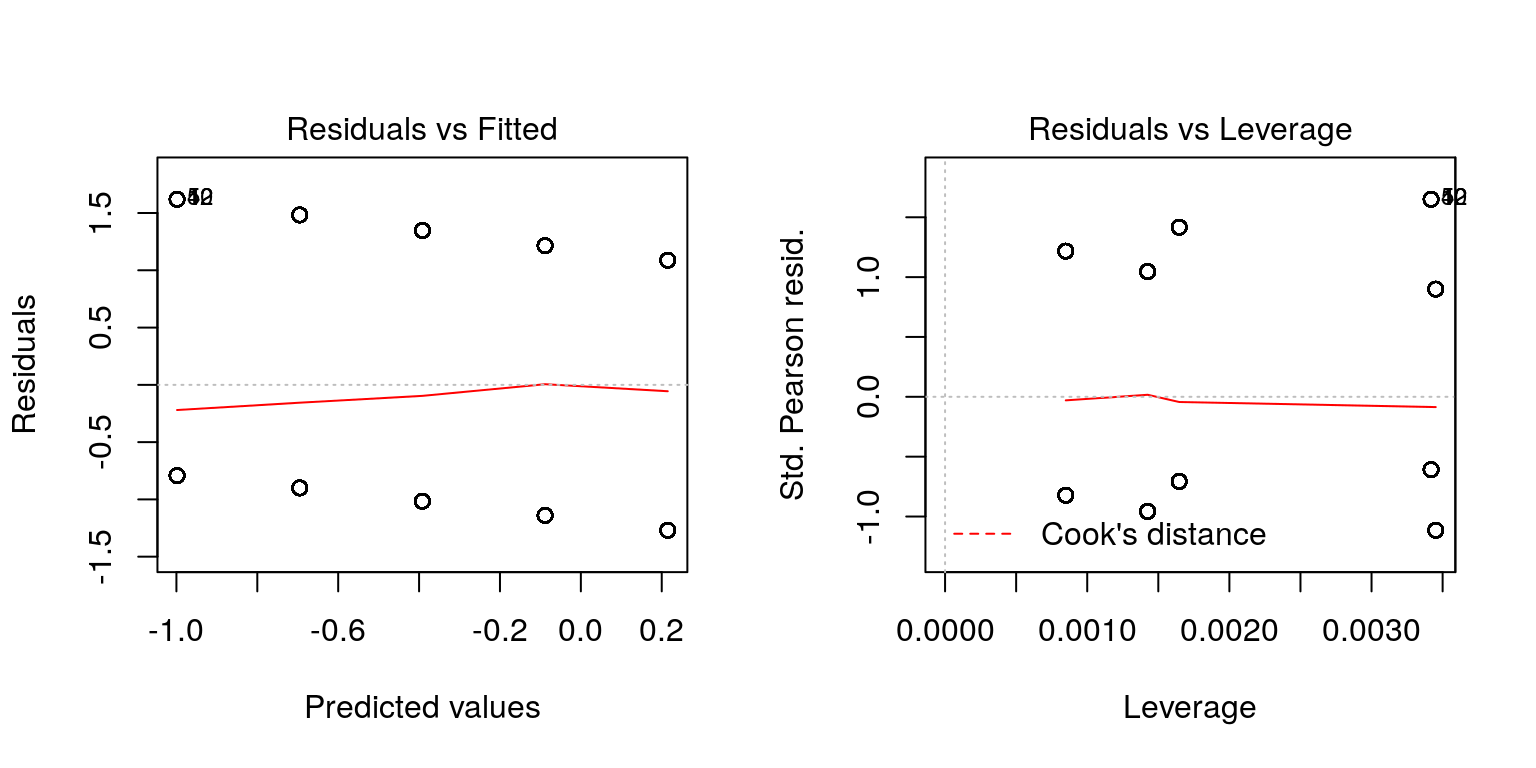
\includegraphics{_main_files/figure-latex/modeldiag-1} \end{center}

Alternative \textbf{residual plots} are possible to generate using the
\texttt{binnedplot()} function in the \texttt{arm} package in R:

\begin{Shaded}
\begin{Highlighting}[]
\NormalTok{USA}\OperatorTok{$}\NormalTok{Vote <-}\StringTok{ }\KeywordTok{ifelse}\NormalTok{(USA}\OperatorTok{$}\NormalTok{Vote }\OperatorTok\StringTok{ 'Bill Clinton'}\NormalTok{, }\DecValTok{0}\NormalTok{, }\DecValTok{1}\NormalTok{) }\CommentTok{# change to 0/1 for plot purposes}
\KeywordTok{library}\NormalTok{(arm)}
\KeywordTok{plot}\NormalTok{(fit, }\DataTypeTok{which =} \DecValTok{1}\NormalTok{)}
\KeywordTok{binnedplot}\NormalTok{(}\KeywordTok{predict}\NormalTok{(fit, }\DataTypeTok{type =} \StringTok{"response"}\NormalTok{), }
\NormalTok{           USA}\OperatorTok{$}\NormalTok{Vote }\OperatorTok{-}\StringTok{ }\KeywordTok{predict}\NormalTok{(fit, }\DataTypeTok{type =} \StringTok{"response"}\NormalTok{))}
\end{Highlighting}
\end{Shaded}

\begin{center}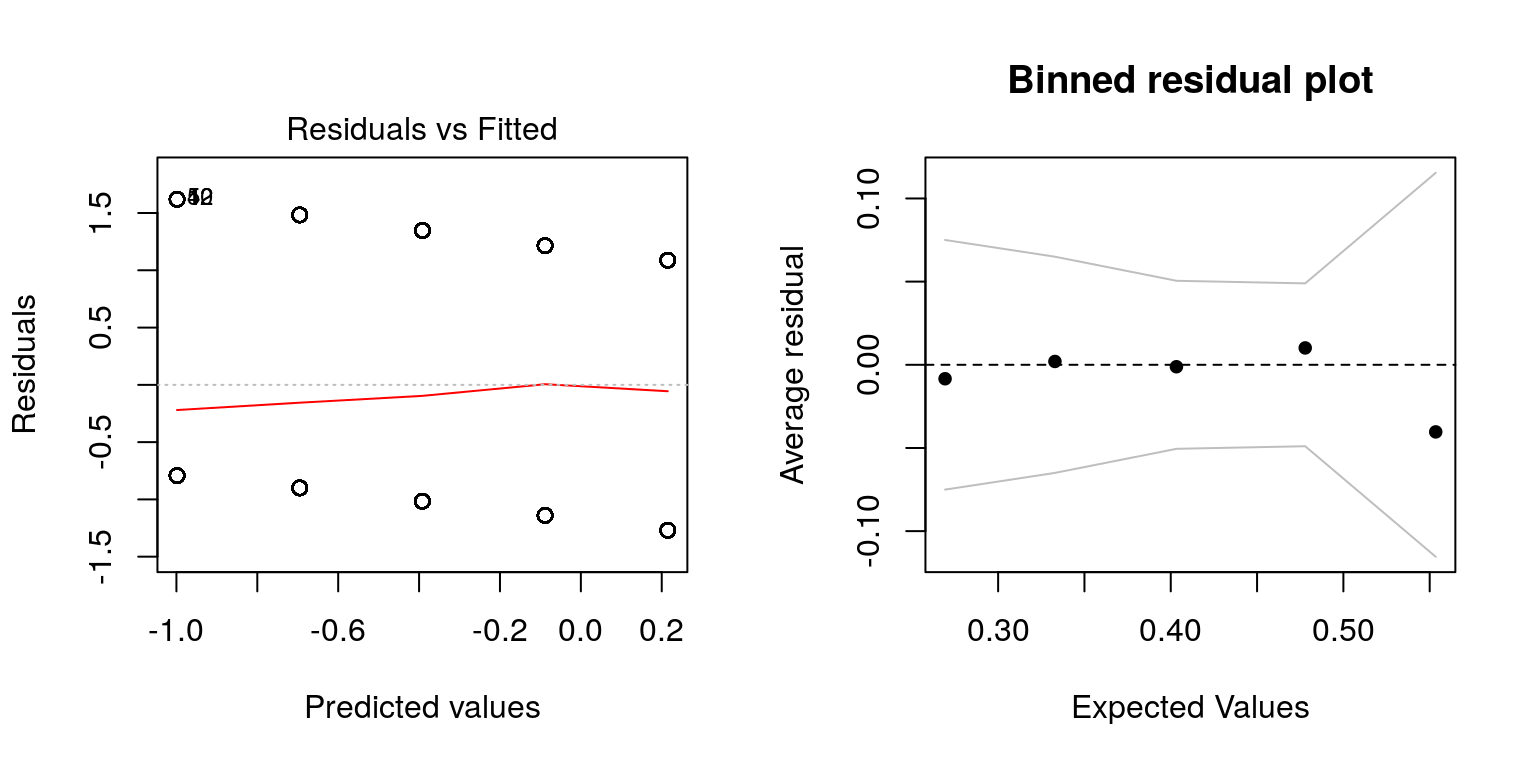
\includegraphics{_main_files/figure-latex/modeldiag1-1} \end{center}

\section{Practical 5 - Wine}\label{practical-5---wine}

The analysis determined the quantities of 13 constituents found in each
of two types of wine. \footnote{the full dataset contains three types of
  wine and is available
  \href{https://archive.ics.uci.edu/ml/datasets/wine}{here}}

Download the data file from
\href{https://exeter-data-analytics.github.io/StatModelling/_data/wine.csv}{here}
and save it to your working directory.

\begin{Shaded}
\begin{Highlighting}[]
\NormalTok{wine <-}\StringTok{ }\KeywordTok{read.csv}\NormalTok{(}\StringTok{"wine.csv"}\NormalTok{, }\DataTypeTok{header=}\NormalTok{T)}
\end{Highlighting}
\end{Shaded}

\begin{Shaded}
\begin{Highlighting}[]
\KeywordTok{head}\NormalTok{(wine)}
\end{Highlighting}
\end{Shaded}

\begin{verbatim}
##   WineType Alcohol MalicAcid  Ash AlcalinityAsh Magnesium TotalPhenols
## 1        A   14.23      1.71 2.43          15.6       127         2.80
## 2        A   13.20      1.78 2.14          11.2       100         2.65
## 3        A   13.16      2.36 2.67          18.6       101         2.80
## 4        A   14.37      1.95 2.50          16.8       113         3.85
## 5        A   13.24      2.59 2.87          21.0       118         2.80
## 6        A   14.20      1.76 2.45          15.2       112         3.27
##   Flavanoids NonflavanoidPhenols Proanthocyanins ColourIntensity  Hue
## 1       3.06                0.28            2.29            5.64 1.04
## 2       2.76                0.26            1.28            4.38 1.05
## 3       3.24                0.30            2.81            5.68 1.03
## 4       3.49                0.24            2.18            7.80 0.86
## 5       2.69                0.39            1.82            4.32 1.04
## 6       3.39                0.34            1.97            6.75 1.05
##   OD280_OD315 Proline
## 1        3.92    1065
## 2        3.40    1050
## 3        3.17    1185
## 4        3.45    1480
## 5        2.93     735
## 6        2.85    1450
\end{verbatim}

The data columns are self-explanatory, but for the purpose of this
practical we will just focus on \texttt{Alcohol} content and
\texttt{TotalPhenols} (a class of chemical compound). The question of
interest is:

\begin{quote}
Can we differentiate between the two types of wine using
\texttt{Alcohol} and \texttt{TotalPhenols}?
\end{quote}

\hypertarget{tsk12}{}\bblockT[Task]{\phantomsection\label{sol12}12}

\begin{enumerate}
\def\labelenumi{\arabic{enumi}.}
\tightlist
\item
  Plot a scatterplot of \texttt{Alcohol} vs \texttt{TotalPhenols} and
  colour data points by \texttt{WineType}
\end{enumerate}

\eblockT

\hyperlink{sol12}{\buttonS{Show Solution on P\colpageref{tsk12}}}

\hypertarget{tsk13}{}\bblockT[Task]{\phantomsection\label{sol13}13}

\begin{enumerate}
\def\labelenumi{\arabic{enumi}.}
\setcounter{enumi}{1}
\tightlist
\item
  Fit a logistic regression model with \texttt{WineType} as response
  variable and \texttt{Alcohol} and \texttt{TotalPhenols} as explanatory
  variables. Display a summary of the fit.
\end{enumerate}

\eblockT

\hyperlink{sol13}{\buttonS{Show Solution on P\colpageref{tsk13}}}

\hypertarget{tsk14}{}\bblockT[Task]{\phantomsection\label{sol14}14}

\begin{enumerate}
\def\labelenumi{\arabic{enumi}.}
\setcounter{enumi}{2}
\tightlist
\item
  What is the probability that a wine with alcohol content of 12.5\% and
  total phenols of 2.5 units, is of \texttt{WineType} B? Hint: Use the
  \texttt{invlogit} function already available in the \texttt{arm}
  package
  (\texttt{install.packages(\textquotesingle{}arm\textquotesingle{})})
\end{enumerate}

\eblockT

\hyperlink{sol14}{\buttonS{Show Solution on P\colpageref{tsk14}}}

\hypertarget{tsk15}{}\bblockT[Task]{\phantomsection\label{sol15}15}

\begin{enumerate}
\def\labelenumi{\arabic{enumi}.}
\setcounter{enumi}{3}
\tightlist
\item
  Plot the mean regression lines on the \textbf{probability scale} for
  \emph{varying} values of \texttt{Alcohol} but fixed values of
  \texttt{TotalPhenols} of 1.5, 2.5 and 3.5 (i.e a plot with
  \texttt{Alcohol} on the x-axis and predicted probability of
  \texttt{WineType} B on the y-axis for the three cases of
  \texttt{TotalPhenols}).
\end{enumerate}

\eblockT

\hyperlink{sol15}{\buttonS{Show Solution on P\colpageref{tsk15}}}

\section{Summary}\label{summary-2}

\textbf{GLMs} are powerful and flexible.

They can be used to fit a wide variety of data types.

Model checking becomes trickier.

Extensions include:

\begin{itemize}
\tightlist
\item
  \textbf{mixed models};
\item
  \textbf{survival models};
\item
  \textbf{generalised additive models} (GAMs).
\end{itemize}

\chapter{Mixed effects models}\label{mixed-effects-models}

My thanks in particular to
\href{http://biosciences.exeter.ac.uk/staff/index.php?web_id=david_hodgson}{Dave
Hodgson}, who's fantastic Master's course offered up the prototype for
this workshop.

Slides can be downloaded from:

\begin{itemize}
\tightlist
\item
  \href{https://exeter-data-analytics.github.io/StatModelling/04-mixed-effects-models-handout.pdf}{(G)LMMs
  in R}
\end{itemize}

Firstly, install if necessary (using \texttt{install.packages()};
uncomment the code below if required) and load the \texttt{lme4}
package:

\begin{Shaded}
\begin{Highlighting}[]
\NormalTok{## load libraries}
\KeywordTok{library}\NormalTok{(tidyverse)}
\KeywordTok{library}\NormalTok{(lme4)}
\end{Highlighting}
\end{Shaded}

\begin{quote}
\textbf{Note}: In this session I will use \texttt{tidyverse} as the
principal way to generate plots etc. because it's \textbf{\emph{far}}
easier for many of the examples in this workshop. The base R code is
provided for those of you that are not familiar with \texttt{tidyverse}.
\end{quote}

This practical will focus on how to analyse data when the experimental
design (or the surveyed explanatory variables) obliges us to study
non-independent experimental units. You will find yourself
distinguishing between random effects and fixed effects. You will find
yourself frustrated at the lack of consensus regarding how to simplify
fixed factors in mixed models. It takes a long time to understand how to
deal with blocks (and other random effects): don't expect understanding
to come overnight, and do rely on books and websites to help you. But be
warned, at this level of statistical prowess, much of the literature is
written in Greek symbols and matrix algebra.

\textbf{\emph{Health Warning: some of these mixed-effects modelling
packages are quickly evolving, and future updates might play some havoc
with the coding, and outputs from, the scripts written here. You will
need to keep your eye on the forums in the future if this happens. As
always, let me or your demonstrators know if you encounter
difficulties.}}

If this workshop has whetted your appetite, then a range of nice
examples can be found at
\href{http://www.maths.bath.ac.uk/~jjf23/}{Julian Faraway's} site:
\url{http://www.maths.bath.ac.uk/~jjf23/mixchange/index.html}. These
examples are discussed in his book:
\href{https://www.amazon.co.uk/Extending-Linear-Model-Generalized-Nonparametric/dp/158488424X}{Extending
the Linear Model with R}.

\section{A note on variable selection and model
simplification}\label{a-note-on-variable-selection-and-model-simplification}

By design we have been a bit wary in focusing on the eponymous null
hypothesis significance testing (NHST) ideas (and associated idolisation
of p-values). We have done this because we want to emphasise that a
statistical model is more than just a p-value, and also that a p-value
on its own (without some measure of effect size) is meaningless. We
appreciate that this might fly in the face of the way that you might
have seen statistical models presented in courses or papers, and this
section is our attempt to explain to you some of the controversies
surrounding these approaches.

There are many philosophical complexities with the way that p-values are
used in many papers, and there have been many papers published
discussing their misuse and misinterpretations. A good one is
\href{https://www.nature.com/articles/nmeth.3288.pdf?origin=ppub}{Halsey
et al. (2015)}.

This is not to say that null hypothesis significance testing (hereafter
NHST) is wrong, it's just that it's easy to misuse, even for experienced
data modellers. Here are some common challenges / misconceptions:

\begin{enumerate}
\def\labelenumi{\arabic{enumi}.}
\tightlist
\item
  A p-value is the \emph{``probability of observing a test statistic
  equal to or more extreme than the observed test statistic if the null
  hypothesis is true''}; it is \textbf{not} the \emph{``probability that
  the null hypothesis is false''}.
\item
  Leads to a binary interpretation: \emph{``is there an effect?''}``,
  rather than, \emph{``what is the size of the effect''}?
\item
  They are heavily dependent on \textbf{sample size}:

  \begin{itemize}
  \tightlist
  \item
    a \emph{larger} study with the same effect size and variance will be
    \emph{more} statistically significant. Example: study is exploring
    differences between sample means from two groups, \(\bar{x}\) and
    \(\bar{y}\).

    \begin{itemize}
    \tightlist
    \item
      \(~~\bar{x} = 10\), \(\bar{y} = 12\), \(s = 5\) (pooled SD),
      \(n = 5\) (per group): \(\mathbf{p = 0.4}\).
    \item
      \(~~\bar{x} = 10\), \(\bar{y} = 12\), \(s = 5\) (pooled SD),
      \(n = 30\) (per group): \(\mathbf{p = 0.0332}\).
    \end{itemize}
  \end{itemize}
\item
  The p-value itself is a \textbf{random variable}, and can have a very
  wide variance

  \begin{itemize}
  \tightlist
  \item
    Geoff Cumming's
    \href{https://www.youtube.com/embed/5OL1RqHrZQ8}{`dance of the
    p-values'}.
  \item
    Type I, II, S and M errors.
  \end{itemize}
\item
  Often, the null hypothesis of a \textbf{zero effect} is not a
  \textbf{biologically} valid one.

  \begin{itemize}
  \tightlist
  \item
    \href{http://www.tandfonline.com/doi/abs/10.1198/000313006X152649}{The
    difference between ``significant'' and ``not significant'' is not
    itself statistically significant\ldots{}}
  \end{itemize}
\item
  Direction and magnitude of effects are important.

  \begin{itemize}
  \tightlist
  \item
    Consider a \textbf{large} study which finds a \textbf{small} effect
    size of \(x\) (\(p < 0.001\)), with the \textbf{minimum biologically
    significant} effect size being \textbf{\emph{larger}} than \(x\).
  \item
    Therefore, the \textbf{\emph{highly (statistically) significant}}
    p-value provides strong evidence of a \textbf{lack-of-effect}. It
    corresponds to a \textbf{negligible real-world} effect estimated
    with high precision!
  \end{itemize}
\end{enumerate}

Many of these problems go away when a study is appropriately
\textbf{powered}, with careful experimental design. In this case the
sample size is large enough to have high power for the comparison of
interest, and the study is often set up in such a way as to make the
comparison of interest meaningful. Note that these kinds of study were
what NHST were derived to model.

That being said, there are times when NHST can be useful, particularly
if you have a complex system (perhaps with large numbers of explanatory
variables), and you wish to produce a more parsimonious model (perhaps
because it is easier to interpret).

\subsection{Common NHST approaches to model
simplification}\label{common-nhst-approaches-to-model-simplification}

Traditionally, if the response variable is Gaussian (normal), then you
may have come across two frequently used approaches:

\begin{itemize}
\tightlist
\item
  F-tests: based on comparing the residual mean squared error with the
  regression mean squared error, or
\item
  Likelihood ratio tests (LRT): based on comparing the model deviance
  between two models.
\end{itemize}

Both of these cases are \textbf{exact} tests for linear regression with
Gaussian errors (but for mixed models these become approximate). Let's
have a look at a simple example using the fruitflies data from earlier
practicals. These data are available in the
\href{https://exeter-data-analytics.github.io/StatModelling/_data/fruitfly.rds}{``fruitfly.rds''}
file.

\begin{Shaded}
\begin{Highlighting}[]
\NormalTok{ff <-}\StringTok{ }\KeywordTok{readRDS}\NormalTok{(}\StringTok{"fruitfly.rds"}\NormalTok{)}
\end{Highlighting}
\end{Shaded}

\newpage

\begin{Shaded}
\begin{Highlighting}[]
\NormalTok{ff_lm <-}\StringTok{ }\KeywordTok{lm}\NormalTok{(longevity }\OperatorTok{~}\StringTok{ }\NormalTok{type, }\DataTypeTok{data =}\NormalTok{ ff)}
\KeywordTok{summary}\NormalTok{(ff_lm)}
\end{Highlighting}
\end{Shaded}

\begin{verbatim}
## 
## Call:
## lm(formula = longevity ~ type, data = ff)
## 
## Residuals:
##    Min     1Q Median     3Q    Max 
## -31.74 -13.74   0.26  11.44  33.26 
## 
## Coefficients:
##                 Estimate Std. Error t value Pr(>|t|)    
## (Intercept)       63.560      3.158  20.130  < 2e-16 ***
## typeInseminated    0.520      3.867   0.134    0.893    
## typeVirgin       -15.820      3.867  -4.091 7.75e-05 ***
## ---
## Signif. codes:  0 '***' 0.001 '**' 0.01 '*' 0.05 '.' 0.1 ' ' 1
## 
## Residual standard error: 15.79 on 122 degrees of freedom
## Multiple R-squared:  0.2051, Adjusted R-squared:  0.1921 
## F-statistic: 15.74 on 2 and 122 DF,  p-value: 8.305e-07
\end{verbatim}

\begin{Shaded}
\begin{Highlighting}[]
\KeywordTok{anova}\NormalTok{(ff_lm, }\DataTypeTok{test =} \StringTok{"F"}\NormalTok{)}
\end{Highlighting}
\end{Shaded}

\begin{verbatim}
## Analysis of Variance Table
## 
## Response: longevity
##            Df  Sum Sq Mean Sq F value    Pr(>F)    
## type        2  7845.3  3922.7  15.738 8.305e-07 ***
## Residuals 122 30407.5   249.2                      
## ---
## Signif. codes:  0 '***' 0.001 '**' 0.01 '*' 0.05 '.' 0.1 ' ' 1
\end{verbatim}

Here the \texttt{anova()} function performs an F-test for the
\texttt{longevity\ \textasciitilde{}\ type} model vs.~the null model
(\texttt{longevity\ \textasciitilde{}\ 1}). The idea is that \emph{if
the fit from the competing models is the same}, then the ratio of mean
squared errors will follow an F-distribution on 2 and 122
degrees-of-freedom (d.f.) in this case.

Here we obtain a test statistic of 15.738, which can be compared against
an F-distribution on 2 and 122 d.f., which gives a p-value of
\(8.3 \times 10^{-7}\) (i.e.~a statistically significant change even at
the 1\% and 0.1\% levels). Thus we would conclude that dropping
\texttt{type} produces a statistically significantly inferior model fit
compared to when it is left in the model.

We can do the same thing but using a likelihood ratio test as:

\begin{Shaded}
\begin{Highlighting}[]
\KeywordTok{anova}\NormalTok{(ff_lm, }\DataTypeTok{test =} \StringTok{"Chisq"}\NormalTok{)}
\end{Highlighting}
\end{Shaded}

\begin{verbatim}
## Analysis of Variance Table
## 
## Response: longevity
##            Df  Sum Sq Mean Sq F value    Pr(>F)    
## type        2  7845.3  3922.7  15.738 8.305e-07 ***
## Residuals 122 30407.5   249.2                      
## ---
## Signif. codes:  0 '***' 0.001 '**' 0.01 '*' 0.05 '.' 0.1 ' ' 1
\end{verbatim}

Here the test statistic produces a p-value of \(5.9 \times 10^{-7}\);
again highly statistically significant even at the 0.1\% level, but
slightly different to the F-test (because they are different tests).
Here we are comparing \(-2 \times\) the difference in log-likelihoods
between the competing models, which under the null hypothesis that the
fits are similar, should follow a chi-squared distribution on 2 d.f.
here (the d.f. is the difference in the number of parameters between the
two nested models). In general, in linear regression with Gaussian
errors the F-test is slightly more powerful than the LRT, but you can
use either.

For Generalised Linear Models (GLMs) with non-Gaussian error structure
the F-test is no longer valid, and the LRT is \textbf{approximate} (the
latter is in fact \textbf{asymptotically chi-squared}, which means that
the approximation gets better for larger sample sizes, but can be
misleading in small samples).

If using F-tests or LRTs to compare models, then the models must be
\textbf{nested} (i.e.~you can get one model to equal the other by fixing
some of the parameters---usually setting coefficients to be zero, as in
the fruitflies example). An alternative is to use something like
Akaike's Information Criterion (AIC), which does not assess statistical
significance and does not require the models to be nested (it is in
essence a measure of predictive accuracy).

For \textbf{mixed models} things get trickier again, and there is much
debate about optimal ways to perform model simplification and
inference---see
\href{https://bbolker.github.io/mixedmodels-misc/glmmFAQ.html}{GLMM FAQ}
for more discussion. A nice description of the types of approaches we
can use in different cases can be found at:

\url{https://rdrr.io/cran/lme4/man/pvalues.html}

A useful quote from the
\href{https://bbolker.github.io/mixedmodels-misc/glmmFAQ.html}{GLMM FAQ}
is:

\begin{quote}
``For special cases that correspond to classical experimental designs
(i.e.~balanced designs that are nested, split-plot, randomized block,
etc.) \ldots{} we can show that the null distributions of particular
ratios of sums of squares follow an F distribution with known numerator
and denominator degrees of freedom (and hence the sampling distributions
of particular contrasts are t-distributed with known df). In more
complicated situations (unbalanced, GLMMs, crossed random effects,
models with temporal or spatial correlation, etc.) it is not in general
clear that the null distribution of the computed ratio of sums of
squares is really an F distribution, for any choice of denominator
degrees of freedom.''
\end{quote}

The developers of \texttt{lme4} recommend (from \textbf{worst} to
\textbf{best})\footnote{see
  \href{https://bbolker.github.io/mixedmodels-misc/glmmFAQ.html}{GLMM
  FAQ}}:

\begin{itemize}
\tightlist
\item
  Wald Z-tests;
\item
  For \textbf{balanced}, \textbf{nested LMMs} where degrees of freedom
  can be computed according to classical rules: Wald t-tests;
\item
  Likelihood ratio test, either by setting up the model so that the
  parameter can be isolated/dropped (via \texttt{anova()} or
  \texttt{drop1()}, or via computing likelihood profiles;
\item
  Markov chain Monte Carlo (MCMC) or \textbf{parametric bootstrap
  confidence intervals}.
\end{itemize}

If I do perform model simplification or variable selection, even then I
would present the final model results in terms of effect sizes and
confidence intervals where possible (or via predictive plots), since
although CIs suffer with some of the same problems as p-values, at least
they focus on the magnitude of the effects. If I have large enough
sample sizes and not too many variables, then it may well be fine just
to fit one model and perform inference from that.

In this workshop we will introduce some common scenarios in which mixed
models can be applied, and give examples of model simplification and
inference in these cases. We will tend to use LRTs and profile
confidence intervals simply because they are easier to compute. A
\protect\hyperlink{parboot}{section} at the end will explore the use of
parametric bootstrapping for those of you who are interested.

\section{Non-independent data: Randomised Complete Block
Design}\label{non-independent-data-randomised-complete-block-design}

Often you will find it impossible to allocate treatments to experimental
units at random because they are structured in time or in space. This
means that units are not independent of each other, hence their
residuals will not be independent, and we have violated an important
assumption of generalised linear modelling (and, indeed, of analysis of
variance). However the recognition of natural structuring in our
population of experimental units can be \textbf{very} useful. If the
experimental design can be stratified so that all units that share a
common `trait' (e.g.~share a corner of a field, or share a single
incubator) can represent one or more full replicate of the proposed
experiment, then we should use this natural structuring to absorb some
of our enemy: noise (also called residual deviance).

An extreme case of using error-absorbers is the Randomised Complete
Block Experimental Design. So-called because it includes blocks, each
block contains a single replicate of the experiment, and experimental
units \textbf{within} blocks are allocated to treatment combinations
\textbf{at random}. The concept is best explained using an example.

A microbiologist wishes to know which of four growth media is best for
rearing large populations of anthrax, quickly. However, this poorly
funded scientist does not own a large enough incubator in which to grow
lots of replicate populations. Instead he requests space in five
different incubators owned by other, better-funded researchers. Each
incubator just has space for four bottles of medium. Our scientist
allocates each growth medium to one bottle per incubator \textbf{at
random}, inoculates with anthrax then monitors population growth rate. A
schematic is given in Figure \ref{fig:bacCabinets}.

\begin{figure}

{\centering 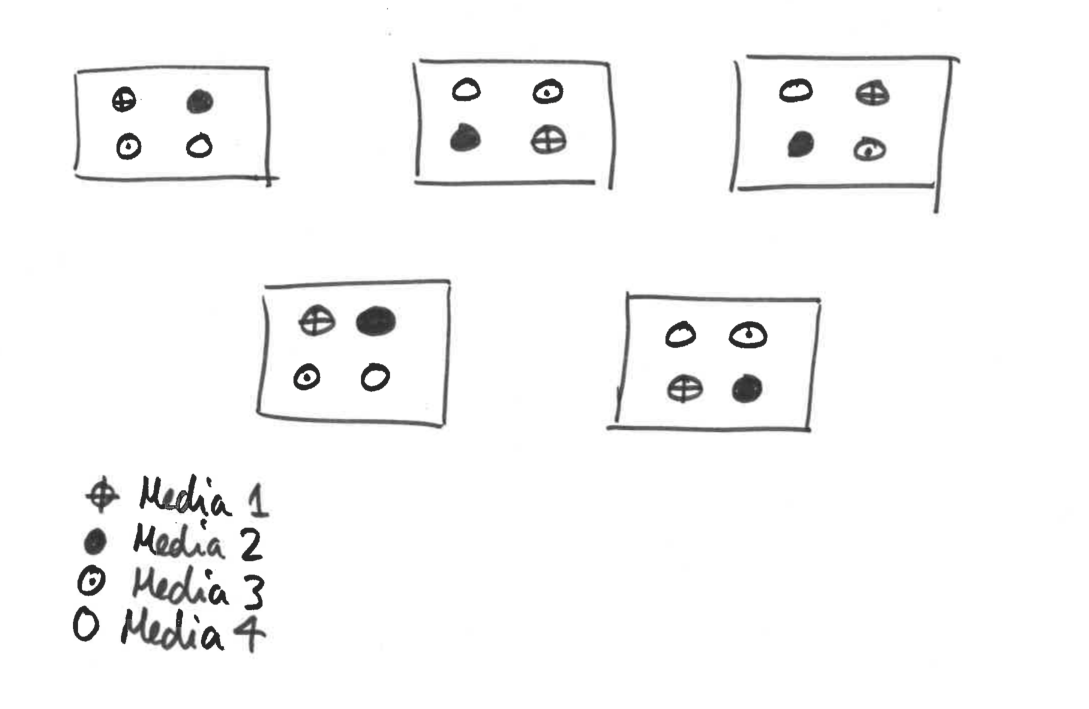
\includegraphics[width=0.8\linewidth,height=0.8\textheight]{_img/bacCabinets} 

}

\caption{Schematic for bacterial growth example}\label{fig:bacCabinets}
\end{figure}

These data are available in the
\href{https://exeter-data-analytics.github.io/StatModelling/_data/bacCabinets.rds}{``bacCabinets.rds''}
file. Read in this dataset and familiarise yourself with its structure.

\begin{Shaded}
\begin{Highlighting}[]
\NormalTok{bac <-}\StringTok{ }\KeywordTok{readRDS}\NormalTok{(}\StringTok{"bacCabinets.rds"}\NormalTok{)}
\end{Highlighting}
\end{Shaded}

Let's do the analysis \textbf{wrongly} to begin with:

\begin{Shaded}
\begin{Highlighting}[]
\NormalTok{bac_lm <-}\StringTok{ }\KeywordTok{lm}\NormalTok{(growth }\OperatorTok{~}\StringTok{ }\NormalTok{media, }\DataTypeTok{data =}\NormalTok{ bac)}
\KeywordTok{drop1}\NormalTok{(bac_lm, }\DataTypeTok{test =} \StringTok{"F"}\NormalTok{)}
\end{Highlighting}
\end{Shaded}

\begin{verbatim}
## Single term deletions
## 
## Model:
## growth ~ media
##        Df Sum of Sq    RSS    AIC F value  Pr(>F)  
## <none>              152.38 48.613                  
## media   3    88.577 240.96 51.778  3.1002 0.05638 .
## ---
## Signif. codes:  0 '***' 0.001 '**' 0.01 '*' 0.05 '.' 0.1 ' ' 1
\end{verbatim}

\hypertarget{tsk16}{}\bblockT[Question]{\phantomsection\label{sol16}16}

Why is this wrong? \eblockT

\hyperlink{sol16}{\buttonS{Show Answer on P\colpageref{tsk16}}}

Let's refit the model with a \texttt{cabinet} effect, and then test for
the statistical significance of \texttt{media}:

\begin{Shaded}
\begin{Highlighting}[]
\NormalTok{bac_lm <-}\StringTok{ }\KeywordTok{lm}\NormalTok{(growth }\OperatorTok{~}\StringTok{ }\NormalTok{media }\OperatorTok{+}\StringTok{ }\NormalTok{cabinet, }\DataTypeTok{data =}\NormalTok{ bac)}
\KeywordTok{drop1}\NormalTok{(bac_lm, }\DataTypeTok{test =} \StringTok{"F"}\NormalTok{)}
\end{Highlighting}
\end{Shaded}

\begin{verbatim}
## Single term deletions
## 
## Model:
## growth ~ media + cabinet
##         Df Sum of Sq    RSS    AIC F value    Pr(>F)    
## <none>                15.23 10.551                      
## media    3    88.577 103.81 42.936  23.264 2.734e-05 ***
## cabinet  4   137.150 152.38 48.613  27.016 6.380e-06 ***
## ---
## Signif. codes:  0 '***' 0.001 '**' 0.01 '*' 0.05 '.' 0.1 ' ' 1
\end{verbatim}

This is better. We need a \texttt{cabinet} effect here to deal with the
fact that measurements within cabinets are not independent. Notice that
the sum-of-squares for \texttt{media} is the same in this model compared
to the one without \texttt{cabinet} in it. This is because we have a
\textbf{balanced design} (i.e.~the same number of measurements in each
combination of explanatory variables). However, the F-statistic is
different, and this is because this depends on the \textbf{residual
sum-of-squares}, which is the second model is different due to the
inclusion of \texttt{cabinet}, which soaks up some of the residual
variance that can be attributed to differences between cabinets.

\begin{quote}
\textbf{Note}: here the \texttt{cabinet} effect \textbf{must} be
included in the model. It does not make sense for us to drop the
\texttt{cabinet} effect and test for whether it should be included or
not. It needs to be included \textbf{by design}! Hence we can ignore the
\texttt{cabinet} line output by \texttt{drop1()}.
\end{quote}

\hypertarget{tsk17}{}\bblockT[Task]{\phantomsection\label{sol17}17}

Try with an \textbf{interaction} effect between \texttt{media} and
\texttt{cabinet}. What happens and why? \eblockT

\hyperlink{sol17}{\buttonS{Show Solution on P\colpageref{tsk17}}}

\newpage

\subsection{Mixed model approach}\label{mixed-model-approach}

Let's re-do this analysis using a \textbf{mixed model}. If you haven't
already, you will need to load the \texttt{lme4} package:

\begin{Shaded}
\begin{Highlighting}[]
\KeywordTok{library}\NormalTok{(lme4)}
\end{Highlighting}
\end{Shaded}

\begin{quote}
\textbf{Fixed and random effects}:

\begin{itemize}
\tightlist
\item
  \texttt{media} is a \textbf{fixed} effect---we chose the media to be
  tested, each media has a specific identity, we want to estimate the
  differences in bacterial growth between different media;
\item
  \texttt{cabinet} is a \textbf{random} effect---we don't care about the
  identity of each cabinet, each cabinet is sampled from a population of
  possible cabinets, we just want to predict and absorb the variance in
  bacterial growth rate explained by cabinet.
\end{itemize}
\end{quote}

Now on with the analysis:

\begin{Shaded}
\begin{Highlighting}[]
\NormalTok{bac_lmer <-}\StringTok{ }\KeywordTok{lmer}\NormalTok{(growth }\OperatorTok{~}\StringTok{ }\NormalTok{media }\OperatorTok{+}\StringTok{ }\NormalTok{(}\DecValTok{1} \OperatorTok{|}\StringTok{ }\NormalTok{cabinet), }\DataTypeTok{data =}\NormalTok{ bac)}
\KeywordTok{summary}\NormalTok{(bac_lmer)}
\end{Highlighting}
\end{Shaded}

\begin{verbatim}
## Linear mixed model fit by REML ['lmerMod']
## Formula: growth ~ media + (1 | cabinet)
##    Data: bac
## 
## REML criterion at convergence: 68.8
## 
## Scaled residuals: 
##     Min      1Q  Median      3Q     Max 
## -1.2306 -0.5407  0.1088  0.4320  1.7696 
## 
## Random effects:
##  Groups   Name        Variance Std.Dev.
##  cabinet  (Intercept) 8.255    2.873   
##  Residual             1.269    1.127   
## Number of obs: 20, groups:  cabinet, 5
## 
## Fixed effects:
##             Estimate Std. Error t value
## (Intercept)   5.5800     1.3801   4.043
## media2        1.7800     0.7125   2.498
## media3       -1.9600     0.7125  -2.751
## media4       -3.8400     0.7125  -5.389
## 
## Correlation of Fixed Effects:
##        (Intr) media2 media3
## media2 -0.258              
## media3 -0.258  0.500       
## media4 -0.258  0.500  0.500
\end{verbatim}

\begin{quote}
\textbf{Syntax for \texttt{lmer}}: The \texttt{lmer} command has two
important sections:

\begin{itemize}
\tightlist
\item
  The first part corresponds to the `fixed effects' part of the model
  (in this case, \texttt{growth\ \textasciitilde{}\ media}), which is
  identical to the model you would enter into \texttt{glm} if there were
  no problems of non-independence of data.
\item
  The second part is where you enter the `random effects' part of the
  model, where you tell R how the data is nested and where the
  non-independence lies. There is a whole world of possibilities here,
  from spatially autocorrelated variance/covariance matrices to
  independently varying random slopes and intercepts. We keep it simple
  in this course. For this example, we assume no interaction between
  media and cabinet, hence we just want to predict and absorb the
  additive variance due to different cabinets. Hence our random effect
  term is \texttt{(1\ \textbar{}\ cabinet)}. This means: `the intercept
  of our linear model will vary according to cabinet'.
\end{itemize}
\end{quote}

Mathematically this corresponds to: \[
    Y_i = \beta_0 + \beta_1 x_{i1} + \beta_2 x_{i2}+ \beta_3 x_{i3} + \gamma_{C_i} + \epsilon_i
\] where \(\epsilon_i \sim N(0, \sigma^2)\), the \(x_{i*}\) are dummy
\textbf{binary} variables corresponding to each level of \texttt{media}.
For example: \[
    x_{i1} = \left\{ \begin{array}{ll}
    1 & \mbox{if measurement $i$ has media = 2}\\
    0 & \mbox{otherwise},
    \end{array}
    \right.
\] and similarly for \(x_{i2}\) and \(x_{i3}\). Here \(\gamma_{C_i}\) is
the random effect term for each \texttt{cabinet}
(\(C_i = 1, \dots, 5\)). The reason why \(\gamma_{C_i}\) are denoted as
\textbf{random} effects, is that we assume they come from some
distribution such that \(\gamma_{j} \sim N(0, \sigma^2_{\gamma})\) (for
\(j = 1, \dots, 5\)). I promise this will be the last equation in these
notes!

\subsubsection{\texorpdfstring{\textbf{REML} vs.
\textbf{ML}}{REML vs. ML}}\label{reml-vs.-ml}

To fit these models we use an approach called \textbf{maximum
likelihood} (\textbf{ML}). ML is a very general technique with desirable
\emph{asymptotic} properties. However, ML estimators can be
\textbf{biased}, particularly for small sample sizes. In mixed models an
alternative approach, known as \textbf{restricted maximum likelihood}
(\textbf{REML}), can be used, which produces better estimates of the
model coefficients, particularly for small sample sizes. However, the
REML likelihood function is different to the ML likelihood function, and
only makes sense for mixed models (since it's designed to estimate the
variance components).

We may have to switch between these two approaches depending on what we
want to do. In general, if you want to compare nested models that only
differ in the random effects, then you can use either REML or ML.
However, if you want to compare models that differ in their fixed
effects, then for \textbf{balanced, nested} designs we can usually
derive suitable tests based on REML fits. For \textbf{unbalanced} or
\textbf{non-nested} designs you will need to use ML. Hence, if we are
performing variable selection or model simplification, then we
\emph{may} have to switch to ML when comparing models, but then refit
the model using REML in order to produce estimates of the coefficients.

\begin{quote}
\textbf{Note:} for various reasons the authors of \texttt{lme4} do not
provide p-values as standard from a call to \texttt{summary()} or
\texttt{anova()}. We can perform a \textbf{likelihood ratio test} for
the impact of dropping \texttt{media} from the fitted model. The
simplest way to do this is to use the \texttt{drop1()} function:

Since this is a \textbf{balanced design}, then we can use either REML or
ML to generate appropriate likelihood ratio tests for assessing the
impact of dropping \textbf{fixed} effects. In an \textbf{unbalanced}
design, then we would need to refit the model using ML. The easiest way
to do this is \emph{in situ}, using the \texttt{update()} function and
setting the argument \texttt{REML\ =\ F}. This does not change the
original \texttt{bac\_lmer} model object.

Trying both approaches here should give the same result.
\end{quote}

\begin{Shaded}
\begin{Highlighting}[]
\KeywordTok{drop1}\NormalTok{(bac_lmer, }\DataTypeTok{test =} \StringTok{"Chisq"}\NormalTok{)}
\end{Highlighting}
\end{Shaded}

\begin{verbatim}
## Single term deletions
## 
## Model:
## growth ~ media + (1 | cabinet)
##        Df     AIC    LRT  Pr(Chi)    
## <none>     85.544                    
## media   3 108.333 28.789 2.48e-06 ***
## ---
## Signif. codes:  0 '***' 0.001 '**' 0.01 '*' 0.05 '.' 0.1 ' ' 1
\end{verbatim}

\begin{Shaded}
\begin{Highlighting}[]
\KeywordTok{drop1}\NormalTok{(}\KeywordTok{update}\NormalTok{(bac_lmer, }\DataTypeTok{REML =}\NormalTok{ F), }\DataTypeTok{test =} \StringTok{"Chisq"}\NormalTok{)}
\end{Highlighting}
\end{Shaded}

\begin{verbatim}
## Single term deletions
## 
## Model:
## growth ~ media + (1 | cabinet)
##        Df     AIC    LRT  Pr(Chi)    
## <none>     85.544                    
## media   3 108.333 28.789 2.48e-06 ***
## ---
## Signif. codes:  0 '***' 0.001 '**' 0.01 '*' 0.05 '.' 0.1 ' ' 1
\end{verbatim}

We have used a \textbf{likelihood ratio test}\footnote{you could also
  use an F-test using the \texttt{Anova()} function in the \texttt{car}
  package in this particular case} to assess whether the removal of
\texttt{media} corresponds to a statistically significantly inferior
model fit, which in this case it does at both the 5\% and 1\% levels.
Hence we should leave \texttt{media} in the model. Once we have the
final model, we can look at a summary of the model fit:

\begin{Shaded}
\begin{Highlighting}[]
\KeywordTok{summary}\NormalTok{(bac_lmer)}
\end{Highlighting}
\end{Shaded}

\begin{verbatim}
## Linear mixed model fit by REML ['lmerMod']
## Formula: growth ~ media + (1 | cabinet)
##    Data: bac
## 
## REML criterion at convergence: 68.8
## 
## Scaled residuals: 
##     Min      1Q  Median      3Q     Max 
## -1.2306 -0.5407  0.1088  0.4320  1.7696 
## 
## Random effects:
##  Groups   Name        Variance Std.Dev.
##  cabinet  (Intercept) 8.255    2.873   
##  Residual             1.269    1.127   
## Number of obs: 20, groups:  cabinet, 5
## 
## Fixed effects:
##             Estimate Std. Error t value
## (Intercept)   5.5800     1.3801   4.043
## media2        1.7800     0.7125   2.498
## media3       -1.9600     0.7125  -2.751
## media4       -3.8400     0.7125  -5.389
## 
## Correlation of Fixed Effects:
##        (Intr) media2 media3
## media2 -0.258              
## media3 -0.258  0.500       
## media4 -0.258  0.500  0.500
\end{verbatim}

\textbf{Note} that this summary has been produced from the model fit
using REML, even though the last LRT was conducted using the model
fitted using ML---this is because we updated the model \emph{in situ}
within \texttt{drop1()}.

The `intercept' of the \texttt{lmer} model is the mean growth rate in
\texttt{media1} for an \textbf{average} cabinet. \texttt{lmer} output
also gives you information criteria about the model, tells you the
standard deviation of the random effects, correlations between levels of
fixed effects, and so on.

\newpage

\begin{quote}
\textbf{Note}: we use a likelihood ratio test (LRT) here, rather than an
F-test. The F-test would be OK in this particular case, with Gaussian
error structure and fully balanced, nested design. However, LRTs are
more general, and thus for consistency I will tend to use these (or AIC)
throughout where required.
\end{quote}

We can derive confidence intervals using \texttt{confint()}, and also
produce predictions from the model using \texttt{predict()}.

\hypertarget{tsk18}{}\bblockT[Task]{\phantomsection\label{sol18}18}

Produce a 97\% confidence interval for each regression coefficient of
the model. What do each of these coefficients mean? \eblockT

\hyperlink{sol18}{\buttonS{Show Solution on P\colpageref{tsk18}}}

\hypertarget{tsk19}{}\bblockT[Task]{\phantomsection\label{sol19}19}

The \texttt{abrasion} data in the \texttt{faraway} package contains
information on an experiment where four materials were fed into a wear
testing machine and the amount of wear recorded. Four samples could be
processed at the same time and the position of these samples may be
important, but we really care about assessing wear rates between
different materials. Multiple runs were performed. You can load the
package and data as follows:

\begin{Shaded}
\begin{Highlighting}[]
\KeywordTok{library}\NormalTok{(faraway)}
\KeywordTok{data}\NormalTok{(abrasion)}
\end{Highlighting}
\end{Shaded}

Take a look at the data and the help file for abrasion (i.e.
\texttt{?abrasion}). Fit an appropriate linear mixed model to these data
and assess whether there is any statistical evidence for differences in
wear rates between the different materials. \eblockT

\hyperlink{sol19}{\buttonS{Show Solution on P\colpageref{tsk19}}}

\section{Non-independent data: pseudoreplication, nested variance and
derived variable
analysis}\label{non-independent-data-pseudoreplication-nested-variance-and-derived-variable-analysis}

We take an example from Sokal \& Rohlf (1981). The experiment involved a
simple one-way anova with 3 treatments given to 6 rats. The analysis was
complicated by the fact that three preparations were taken from the
liver of each rat, and two readings of glycogen content were taken from
each preparation. This generated 6 pseudoreplicates per rat to give a
total of 36 readings in all. A schematic is given in Figure
\ref{fig:rats}.

\begin{figure}

{\centering 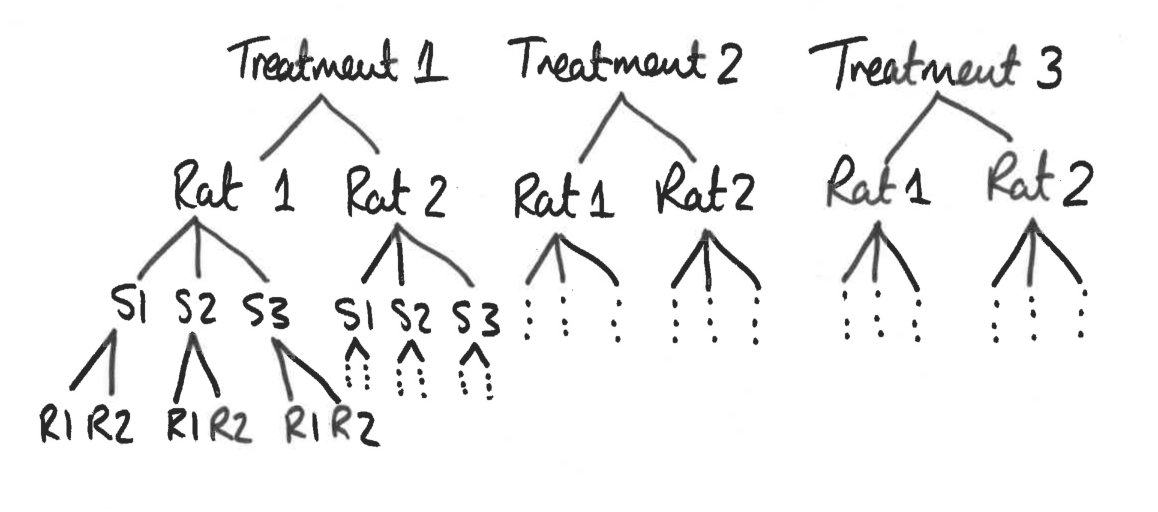
\includegraphics[width=0.8\linewidth,height=0.8\textheight]{_img/rats} 

}

\caption{Schematic for glycogen in rats example}\label{fig:rats}
\end{figure}

Clearly, it would be a mistake to analyse these data as if they were a
straightforward one-way anova, because that would give us 33 degrees of
freedom for error. In fact, since there are only two rats in each
treatment, we have only one degree of freedom per treatment, giving a
total of 3 d.f. for error.

The variance is likely to be different at each level of this nested
analysis because:

\begin{enumerate}
\def\labelenumi{\arabic{enumi}.}
\tightlist
\item
  the readings differ because of variation in the glycogen detection
  method within each liver sample (measurement error);
\item
  the pieces of liver may differ because of heterogeneity in the
  distribution of glycogen within the liver of a single rat;
\item
  the rats will differ from one another in their glycogen levels because
  of sex, age, size, genotype, etc.;
\item
  rats allocated different experimental treatments may differ as a
  result of the fixed effects of treatment.
\end{enumerate}

If all we want to test is whether the experimental treatments have
affected the glycogen levels, then we are not interested in liver bits
within rat's livers, or in preparations within liver bits. We could
combine all the pseudoreplicates together, and analyse the 6 averages.
This would have the virtue of showing what a tiny experiment this really
was. This latter approach also ignores the nested sources of
uncertainties. Instead we will use a linear mixed model.

The new concept here is that there are multiple random effects that are
\textbf{nested}. These data are available in the
\href{https://exeter-data-analytics.github.io/StatModelling/_data/rats.rds}{``rats.rds''}
file. First, read in the data:

\begin{Shaded}
\begin{Highlighting}[]
\NormalTok{rats <-}\StringTok{ }\KeywordTok{readRDS}\NormalTok{(}\StringTok{"rats.rds"}\NormalTok{)}
\KeywordTok{summary}\NormalTok{(rats)}
\end{Highlighting}
\end{Shaded}

\begin{verbatim}
##     Glycogen     Treatment Rat    Liver 
##  Min.   :125.0   1:12      1:18   1:12  
##  1st Qu.:135.8   2:12      2:18   2:12  
##  Median :141.0   3:12             3:12  
##  Mean   :142.2                          
##  3rd Qu.:150.0                          
##  Max.   :162.0
\end{verbatim}

\subsection{The Wrong Analysis}\label{the-wrong-analysis}

Here is what not to do (try it anyway)!

\begin{Shaded}
\begin{Highlighting}[]
\NormalTok{rats_lm <-}\StringTok{ }\KeywordTok{lm}\NormalTok{(Glycogen }\OperatorTok{~}\StringTok{ }\NormalTok{Treatment }\OperatorTok{*}\StringTok{ }\NormalTok{Rat }\OperatorTok{*}\StringTok{ }\NormalTok{Liver, }\DataTypeTok{data =}\NormalTok{ rats)}
\end{Highlighting}
\end{Shaded}

The model has been specified as if it were a full factorial with no
nesting and no pseudoreplication. Note that the structure of the data
allows this mistake to be made. It is a very common problem with data
frames that include pseudoreplication.

\newpage

An ANOVA table gives:

\begin{Shaded}
\begin{Highlighting}[]
\KeywordTok{anova}\NormalTok{(rats_lm, }\DataTypeTok{test =} \StringTok{"F"}\NormalTok{)}
\end{Highlighting}
\end{Shaded}

\begin{verbatim}
## Analysis of Variance Table
## 
## Response: Glycogen
##                     Df  Sum Sq Mean Sq F value    Pr(>F)    
## Treatment            2 1557.56  778.78 36.7927 4.375e-07 ***
## Rat                  1  413.44  413.44 19.5328 0.0003308 ***
## Liver                2  113.56   56.78  2.6824 0.0955848 .  
## Treatment:Rat        2  384.22  192.11  9.0761 0.0018803 ** 
## Treatment:Liver      4  328.11   82.03  3.8753 0.0192714 *  
## Rat:Liver            2   50.89   25.44  1.2021 0.3235761    
## Treatment:Rat:Liver  4  101.44   25.36  1.1982 0.3455924    
## Residuals           18  381.00   21.17                      
## ---
## Signif. codes:  0 '***' 0.001 '**' 0.01 '*' 0.05 '.' 0.1 ' ' 1
\end{verbatim}

\begin{quote}
\textbf{Note}: I can only use the \texttt{anova()} function in this way
because the data are \textbf{balanced} (or at least the model
formulation above with no nesting and no pseudoreplication ends up
treating the data as if they were balanced). In general you have to be
very careful to use \texttt{anova()} in this way.
\end{quote}

This says that there was a highly statistically significant difference
between the treatment means, at least some of the rats were
statistically significantly different from one another, and there was a
statistically significant interaction effect between treatments and
rats. \textbf{This is wrong!} The analysis is flawed because it is based
on the assumption that there is only one error variance and that its
value is 21.2. This value is actually the measurement error; that is to
say the variation between one reading and another from the same piece of
liver. For testing whether the treatment has had any effect, it is the
rats that are the replicates, and there were only 6 of them in the whole
experiment. Note also that the way the rats have been coded makes it
look like there are only two rat ``groups''. Again this is wrong (see
\protect\hyperlink{secmixed}{mixed models} section below).

One way that we could analyse these data is to use a \textbf{derived
variable} analysis.

\subsection{Derived variables avoid
pseudoreplication}\label{derived-variables-avoid-pseudoreplication}

The idea is to get rid of the pseudoreplication by averaging over the
liver bits and preparations for each rat. A useful way of averaging, in
R, is to use \texttt{aggregate} (or \texttt{tidyverse}):

\bmp
\bblockST{\texttt{tidyverse}}

\begin{Shaded}
\begin{Highlighting}[]
\NormalTok{ratsNew <-}\StringTok{ }\NormalTok{rats }\OperatorTok
\StringTok{    }\KeywordTok{group_by}\NormalTok{(Rat, Treatment) }\OperatorTok
\StringTok{    }\KeywordTok{summarise}\NormalTok{(}\DataTypeTok{Glycogen =} \KeywordTok{mean}\NormalTok{(Glycogen))}
\NormalTok{ratsNew}
\end{Highlighting}
\end{Shaded}

\begin{verbatim}
## # A tibble: 6 x 3
## # Groups:   Rat [?]
##   Rat   Treatment Glycogen
##   <fct> <fct>        <dbl>
## 1 1     1             132.
## 2 1     2             150.
## 3 1     3             134.
## 4 2     1             148.
## 5 2     2             152.
## 6 2     3             136
\end{verbatim}

\eblockST
\emp
\hspace{0.01\textwidth} \bmp\bblockST{Base R}

\begin{Shaded}
\begin{Highlighting}[]
\NormalTok{ratsNew <-}\StringTok{ }\KeywordTok{aggregate}\NormalTok{(Glycogen }\OperatorTok{~}\StringTok{ }\NormalTok{Rat }\OperatorTok{+}\StringTok{ }
\StringTok{    }\NormalTok{Treatment, }\DataTypeTok{data =}\NormalTok{ rats, mean)}
\NormalTok{ratsNew}
\end{Highlighting}
\end{Shaded}

\begin{verbatim}
##   Rat Treatment Glycogen
## 1   1         1 132.5000
## 2   2         1 148.5000
## 3   1         2 149.6667
## 4   2         2 152.3333
## 5   1         3 134.3333
## 6   2         3 136.0000
\end{verbatim}

\eblockST
\emp

Here, \texttt{ratsNew} is a new dataset (hopefully shorter than its
ancestral dataset) but has the same column headings as \texttt{rats}.
(Hence be careful to specify the \textbf{correct} data set using the
\texttt{data} argument where necessary.)

\begin{Shaded}
\begin{Highlighting}[]
\NormalTok{ratsNew_lm <-}\StringTok{ }\KeywordTok{lm}\NormalTok{(Glycogen }\OperatorTok{~}\StringTok{ }\NormalTok{Treatment, }\DataTypeTok{data =}\NormalTok{ ratsNew)}
\KeywordTok{drop1}\NormalTok{(ratsNew_lm, }\DataTypeTok{test =} \StringTok{"F"}\NormalTok{)}
\end{Highlighting}
\end{Shaded}

\begin{verbatim}
## Single term deletions
## 
## Model:
## Glycogen ~ Treatment
##           Df Sum of Sq    RSS    AIC F value Pr(>F)
## <none>                 132.94 24.589               
## Treatment  2    259.59 392.54 27.085   2.929 0.1971
\end{verbatim}

This is a statistically valid analysis, but it ignores the uncertainties
around the pseudo-replicates, and the interpretation of the response
variable is actually the mean of a bunch of measurements, not the
measurements themselves. In balanced designs this is OK, but it may not
be possible to generate derived variables for some studies (how do you
average a categorical response for example)?

\hypertarget{secmixed}{\subsection{Mixed model
approach}\label{secmixed}}

\subsubsection{Nested and crossed random
effects}\label{nested-and-crossed-random-effects}

The bacterial loads example we saw earlier is an example of a
\textbf{crossed} random effect i.e.~the \texttt{cabinet} level
\texttt{1} corresponds to the \textbf{same} cabinet for each of the
\texttt{media} levels. In the \texttt{rats} data set this is no longer
so, and we have to be careful to get the model formula correct.
\textbf{This section is subtle but important!}

Notice that in the \texttt{rats} data the \texttt{Rat} column is coded
as a \texttt{1} or a \texttt{2}. This means that we could use the
formula:

\begin{Shaded}
\begin{Highlighting}[]
\NormalTok{rats_lmer <-}\StringTok{ }\KeywordTok{lmer}\NormalTok{(Glycogen }\OperatorTok{~}\StringTok{ }\NormalTok{Treatment }\OperatorTok{+}\StringTok{ }\NormalTok{(}\DecValTok{1} \OperatorTok{|}\StringTok{ }\NormalTok{Rat), }\DataTypeTok{data =}\NormalTok{ rats)}
\end{Highlighting}
\end{Shaded}

\textbf{without} throwing an error.

\hypertarget{tsk20}{}\bblockT[Question]{\phantomsection\label{sol20}20}

Why is this wrong? \eblockT

\hyperlink{sol20}{\buttonS{Show Answer on P\colpageref{tsk20}}}

In this case we must tell \texttt{lmer()} that \texttt{Liver} is
\textbf{nested} within \texttt{Rat}, and \texttt{Rat} within
\texttt{Treatment}. We can do this in various ways, but the easiest
thing here is to generate a unique coding for each of the 6 rats.

\bmp
\bblockST{\texttt{tidyverse}}

\begin{Shaded}
\begin{Highlighting}[]
\NormalTok{rats <-}\StringTok{ }\NormalTok{rats }\OperatorTok
\StringTok{    }\KeywordTok{unite}\NormalTok{(Rat, Treatment, Rat, }
          \DataTypeTok{sep =} \StringTok{"_"}\NormalTok{, }\DataTypeTok{remove =}\NormalTok{ F) }\OperatorTok
\StringTok{    }\KeywordTok{mutate}\NormalTok{(}\DataTypeTok{Rat =} \KeywordTok{factor}\NormalTok{(}
        \KeywordTok{as.numeric}\NormalTok{(}\KeywordTok{factor}\NormalTok{(Rat))))}
\end{Highlighting}
\end{Shaded}

\eblockST
\emp
\hspace{0.01\textwidth} \bmp\bblockST{Base R}

\begin{Shaded}
\begin{Highlighting}[]
\NormalTok{rats}\OperatorTok{$}\NormalTok{Rat <-}\StringTok{ }\KeywordTok{paste}\NormalTok{(rats}\OperatorTok{$}\NormalTok{Treatment, }
    \StringTok{"_"}\NormalTok{, rats}\OperatorTok{$}\NormalTok{Rat)}
\NormalTok{rats}\OperatorTok{$}\NormalTok{Rat <-}\StringTok{ }\KeywordTok{factor}\NormalTok{(}
    \KeywordTok{as.numeric}\NormalTok{(}\KeywordTok{factor}\NormalTok{(rats}\OperatorTok{$}\NormalTok{Rat)))}
\end{Highlighting}
\end{Shaded}

\eblockST
\emp

We can use \textbf{nested} random effects to account for the hierarchy
of measurements:

\begin{Shaded}
\begin{Highlighting}[]
\NormalTok{rats_lmer <-}\StringTok{ }\KeywordTok{lmer}\NormalTok{(Glycogen }\OperatorTok{~}\StringTok{ }\NormalTok{Treatment }\OperatorTok{+}\StringTok{ }\NormalTok{(}\DecValTok{1} \OperatorTok{|}\StringTok{ }\NormalTok{Rat }\OperatorTok{/}\StringTok{ }\NormalTok{Liver), }\DataTypeTok{data =}\NormalTok{ rats)}
\KeywordTok{drop1}\NormalTok{(}\KeywordTok{update}\NormalTok{(rats_lmer, }\DataTypeTok{REML =}\NormalTok{ F), }\DataTypeTok{test =} \StringTok{"Chisq"}\NormalTok{)}
\end{Highlighting}
\end{Shaded}

\begin{verbatim}
## Single term deletions
## 
## Model:
## Glycogen ~ Treatment + (1 | Rat/Liver)
##           Df    AIC    LRT Pr(Chi)  
## <none>       245.27                 
## Treatment  2 247.77 6.4962 0.03885 *
## ---
## Signif. codes:  0 '***' 0.001 '**' 0.01 '*' 0.05 '.' 0.1 ' ' 1
\end{verbatim}

\begin{quote}
\textbf{Note}: the syntax \texttt{Rats\ /\ Liver} means that the
\texttt{Liver} levels are \textbf{nested} within the \texttt{Rat}
levels. In this case we do not have to recode \texttt{Liver} to be
unique, since the nesting ensures that \texttt{lmer()} knows that
\texttt{Liver\ =\ 1} inside \texttt{Rat\ =\ 1} is different from
\texttt{Liver\ =\ 1} inside \texttt{Rat\ =\ 2}.
\end{quote}

\hypertarget{tsk21}{}\bblockT[Task]{\phantomsection\label{sol21}21}

The data for the alcohol example in the slides can be found in the
\href{https://exeter-data-analytics.github.io/StatModelling/_data/drunk.rds}{``drunk.rds''}
file. Read this data set into R and:

\begin{enumerate}
\def\labelenumi{\arabic{enumi}.}
\tightlist
\item
  Conduct a derived variable analysis, to test for the impact of
  \texttt{freshener} use on the model fit using a likelihood ratio test.
\item
  Produce 97\% confidence intervals for the \texttt{freshener} effect.
\item
  Fit a mixed model using \texttt{lmer()}, taking care to get the
  nesting of the random effects correct.
\item
  Use a likelihood ratio test to assess the impact of \texttt{freshener}
  on the model fit. Does it matter whether you use REML or ML here, and
  why?
\item
  Produce an estimate of the \texttt{freshener} effect with 97\% profile
  confidence intervals.
\item
  How do these estimates compare?
\end{enumerate}

\eblockT

\hyperlink{sol21}{\buttonS{Show Solution on P\colpageref{tsk21}}}

\section{Non-independent data: Split-plot
analyses}\label{non-independent-data-split-plot-analyses}

Split-plot experiments are like nested designs in that they involve
plots of different sizes and hence have multiple error terms (one error
term for each plot size). They are also like nested designs in that they
involve pseudoreplication: measurements made on the smaller plots are
pseudoreplicates as far as the treatments applied to larger plots are
concerned. This is spatial pseudoreplication, and arises because the
smaller plots nested within the larger plots are not spatially
independent of one another. The only real difference between nested
analysis and split plot analysis is that other than blocks, all of the
factors in a split-plot experiment are typically fixed effects, whereas
in most nested analyses most (or all) of the factors are random effects.

This experiment involves the yield of cereals in a factorial experiment
with 3 treatments, each applied to plots of different sizes within 4
blocks. The largest plots (half of each block) were irrigated or not
because of the practical difficulties of watering large numbers of small
plots. Next, the irrigated plots were split into 3 smaller split-plots
and seeds were sown at different densities. Again, because the seeds
were machine sown, larger plots were preferred. Finally, each sowing
density plot was split into 3 small split-split plots and fertilisers
applied by hand (N alone, P alone and N + P together). A schematic is
given in Figure \ref{fig:splityields}.

\begin{figure}

{\centering 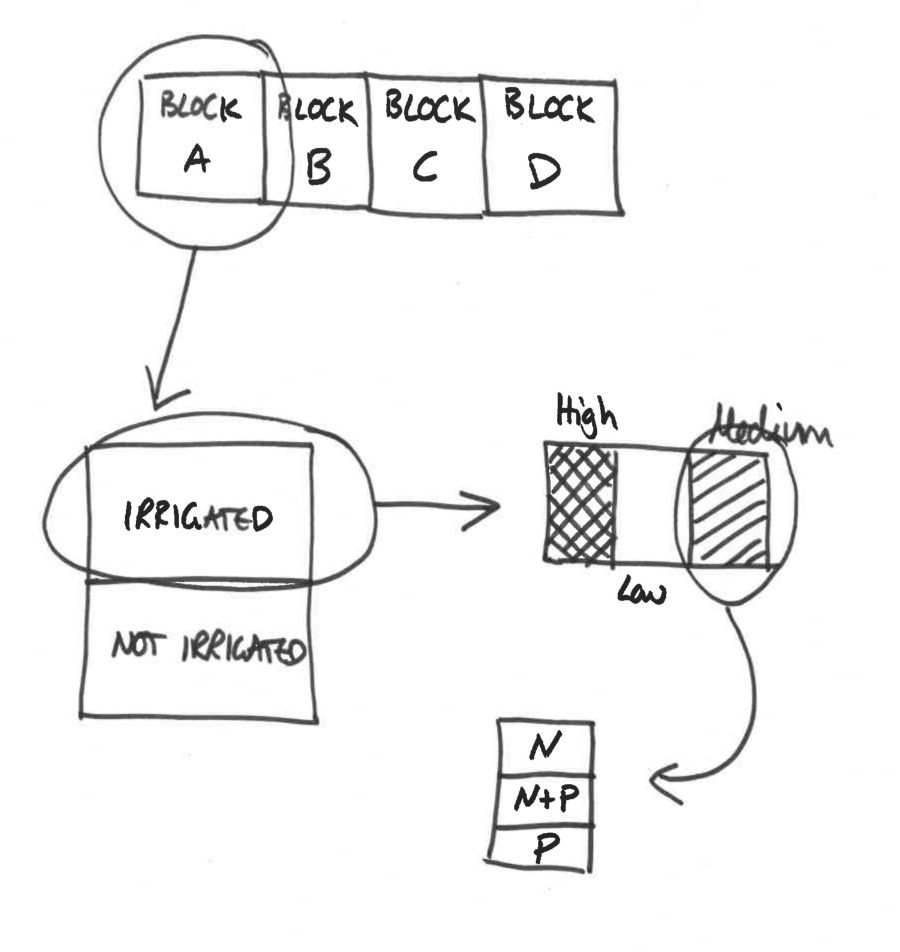
\includegraphics[width=0.8\linewidth,height=0.8\textheight]{_img/splitPlot} 

}

\caption{Schematic for split plot example}\label{fig:splityields}
\end{figure}

\newpage

The data look like:

\begin{longtable}[]{@{}cccccccc@{}}
\toprule
~ & ~ & ~ & Control & ~ & ~ & Irrigated & ~\tabularnewline
\midrule
\endhead
& \textbf{Density / Fertiliser} & N & NP & P & N & NP & P\tabularnewline
& high & 81 & 93 & 92 & 78 & 122 & 98\tabularnewline
\textbf{Block A} & medium & 92 & 92 & 89 & 121 & 119 &
110\tabularnewline
& low & 90 & 107 & 95 & 80 & 100 & 87\tabularnewline
& high & 74 & 74 & 81 & 136 & 132 & 133\tabularnewline
\textbf{Block B} & medium & 98 & 106 & 98 & 99 & 123 & 94\tabularnewline
& low & 83 & 95 & 80 & 102 & 105 & 109\tabularnewline
& high & 82 & 94 & 78 & 119 & 136 & 122\tabularnewline
\textbf{Block C} & medium & 112 & 91 & 104 & 90 & 113 &
118\tabularnewline
& low & 85 & 88 & 88 & 60 & 114 & 104\tabularnewline
& high & 85 & 83 & 89 & 116 & 133 & 136\tabularnewline
\textbf{Block D} & medium & 79 & 87 & 86 & 109 & 126 &
131\tabularnewline
& low & 86 & 89 & 78 & 73 & 114 & 114\tabularnewline
\bottomrule
\end{longtable}

These data are available in the
\href{https://exeter-data-analytics.github.io/StatModelling/_data/splityield.rds}{``splityield.rds''}
file. First, let's read in the data and take a look at it.

\begin{Shaded}
\begin{Highlighting}[]
\NormalTok{splityield <-}\StringTok{ }\KeywordTok{readRDS}\NormalTok{(}\StringTok{"splityield.rds"}\NormalTok{)}
\KeywordTok{head}\NormalTok{(splityield)}
\KeywordTok{summary}\NormalTok{(splityield)}
\end{Highlighting}
\end{Shaded}

\begin{verbatim}
##   yield block irrigation density fertilizer
## 1    90     A    control     low          N
## 2    95     A    control     low          P
## 3   107     A    control     low         NP
## 4    92     A    control  medium          N
## 5    89     A    control  medium          P
## 6    92     A    control  medium         NP
\end{verbatim}

\begin{verbatim}
##      yield        block      irrigation   density   fertilizer
##  Min.   : 60.00   A:18   control  :36   high  :24   N :24     
##  1st Qu.: 86.00   B:18   irrigated:36   medium:24   NP:24     
##  Median : 95.00   C:18                  low   :24   P :24     
##  Mean   : 99.72   D:18                                        
##  3rd Qu.:114.00                                               
##  Max.   :136.00
\end{verbatim}

\subsection{\texorpdfstring{Analysing split-plot designs using
\texttt{lmer}}{Analysing split-plot designs using lmer}}\label{analysing-split-plot-designs-using-lmer}

Now, how do we set up a mixed effects model to analyse these data?
\texttt{block} is the only random effect but our data are nested. Our
fixed effects are \texttt{irrigation}, \texttt{density} and
\texttt{fertilizer}. Here is the model, including prediction of the
variance due to block's random effect on the intercept of the model.

\textbf{Note}: Ordinarily we would write the nested random effect terms
using the syntax:

\begin{Shaded}
\begin{Highlighting}[]
\NormalTok{split_lmer <-}\StringTok{ }\KeywordTok{lmer}\NormalTok{(yield }\OperatorTok{~}\StringTok{ }\NormalTok{irrigation }\OperatorTok{*}\StringTok{ }\NormalTok{density }\OperatorTok{*}\StringTok{ }\NormalTok{fertilizer }\OperatorTok{+}\StringTok{ }
\StringTok{                       }\NormalTok{(}\DecValTok{1} \OperatorTok{|}\StringTok{ }\NormalTok{block }\OperatorTok{/}\StringTok{ }\NormalTok{irrigation }\OperatorTok{/}\StringTok{ }\NormalTok{density }\OperatorTok{/}\StringTok{ }\NormalTok{fertilizer), }\DataTypeTok{data =}\NormalTok{ splityield)}
\end{Highlighting}
\end{Shaded}

\begin{verbatim}
## Error: number of levels of each grouping factor must be < number of observations
\end{verbatim}

However, if you run this, you will notice that the function returns an
error. This is because there are no replicates within the final nesting
(i.e.~the table above on has a single replicate in each cell). To
overcome this we need to remove the final nesting. Hence we can run:

\begin{Shaded}
\begin{Highlighting}[]
\NormalTok{split_lmer <-}\StringTok{ }\KeywordTok{lmer}\NormalTok{(yield }\OperatorTok{~}\StringTok{ }\NormalTok{irrigation }\OperatorTok{*}\StringTok{ }\NormalTok{density }\OperatorTok{*}\StringTok{ }\NormalTok{fertilizer }\OperatorTok{+}\StringTok{ }
\StringTok{                       }\NormalTok{(}\DecValTok{1} \OperatorTok{|}\StringTok{ }\NormalTok{block }\OperatorTok{/}\StringTok{ }\NormalTok{irrigation }\OperatorTok{/}\StringTok{ }\NormalTok{density), }\DataTypeTok{data =}\NormalTok{ splityield)}
\end{Highlighting}
\end{Shaded}

\begin{quote}
\textbf{Aside:} Another way of writing
\texttt{(1\ \textbar{}\ block\ /\ irrigation\ /\ density\ /\ fertilizer)}
is:

\texttt{(1\ \textbar{}\ block)\ +\ (1\ \textbar{}\ block:irrigation)\ +\ (1\ \textbar{}\ block:irrigation:density)\ +\ (1\ \textbar{}\ block:irrigation:density:fertilizer)}.

Pretty grim eh? However, in this case we note that the final nested
random effect only has one replicate per group, so we could simply
remove this term. Leaving:

\texttt{(1\ \textbar{}\ block)\ +\ (1\ \textbar{}\ block:irrigation)\ +\ (1\ \textbar{}\ block:irrigation:density)}.

This is equivalent to
\texttt{(1\ \textbar{}\ block\ /\ irrigation\ /\ density)}
\end{quote}

We can now perform model simplification (remembering to refit the model
using ML in each case):

\begin{Shaded}
\begin{Highlighting}[]
\KeywordTok{drop1}\NormalTok{(}\KeywordTok{update}\NormalTok{(split_lmer, }\DataTypeTok{REML =}\NormalTok{ F), }\DataTypeTok{test =} \StringTok{"Chisq"}\NormalTok{)}
\end{Highlighting}
\end{Shaded}

\begin{verbatim}
## Single term deletions
## 
## Model:
## yield ~ irrigation * density * fertilizer + (1 | block/irrigation/density)
##                               Df    AIC    LRT Pr(Chi)
## <none>                           573.51               
## irrigation:density:fertilizer  4 569.00 3.4938  0.4788
\end{verbatim}

We can see that the three-way interaction term is not statistically
significant, so we can drop it from the model and then test dropping the
two-way interaction effects.

\begin{Shaded}
\begin{Highlighting}[]
\NormalTok{split_lmer <-}\StringTok{ }\KeywordTok{update}\NormalTok{(split_lmer, }\OperatorTok{~}\StringTok{ }\NormalTok{. }\OperatorTok{-}\StringTok{ }\NormalTok{irrigation}\OperatorTok{:}\NormalTok{density}\OperatorTok{:}\NormalTok{fertilizer)}
\KeywordTok{drop1}\NormalTok{(}\KeywordTok{update}\NormalTok{(split_lmer, }\DataTypeTok{REML =}\NormalTok{ F), }\DataTypeTok{test =} \StringTok{"Chisq"}\NormalTok{)}
\end{Highlighting}
\end{Shaded}

\begin{verbatim}
## Single term deletions
## 
## Model:
## yield ~ irrigation + density + fertilizer + (1 | block/irrigation/density) + 
##     irrigation:density + irrigation:fertilizer + density:fertilizer
##                       Df    AIC     LRT  Pr(Chi)   
## <none>                   569.00                    
## irrigation:density     2 576.71 11.7088 0.002867 **
## irrigation:fertilizer  2 577.05 12.0424 0.002427 **
## density:fertilizer     4 565.19  4.1888 0.381061   
## ---
## Signif. codes:  0 '***' 0.001 '**' 0.01 '*' 0.05 '.' 0.1 ' ' 1
\end{verbatim}

We are thus safe to remove the \texttt{density:fertilizer} interaction
term:

\begin{Shaded}
\begin{Highlighting}[]
\NormalTok{split_lmer <-}\StringTok{ }\KeywordTok{update}\NormalTok{(split_lmer, }\OperatorTok{~}\StringTok{ }\NormalTok{. }\OperatorTok{-}\StringTok{ }\NormalTok{density}\OperatorTok{:}\NormalTok{fertilizer)}
\end{Highlighting}
\end{Shaded}

\newpage

\begin{Shaded}
\begin{Highlighting}[]
\KeywordTok{drop1}\NormalTok{(}\KeywordTok{update}\NormalTok{(split_lmer, }\DataTypeTok{REML =}\NormalTok{ F), }\DataTypeTok{test =} \StringTok{"Chisq"}\NormalTok{)}
\end{Highlighting}
\end{Shaded}

\begin{verbatim}
## Single term deletions
## 
## Model:
## yield ~ irrigation + density + fertilizer + (1 | block/irrigation/density) + 
##     irrigation:density + irrigation:fertilizer
##                       Df    AIC    LRT  Pr(Chi)   
## <none>                   565.19                   
## irrigation:density     2 572.90 11.709 0.002867 **
## irrigation:fertilizer  2 572.34 11.144 0.003803 **
## ---
## Signif. codes:  0 '***' 0.001 '**' 0.01 '*' 0.05 '.' 0.1 ' ' 1
\end{verbatim}

We thus have a simplified final model. If you really want to know all
the coefficients, type \texttt{summary(split.lmer)}, but here we will
try to understand the interaction terms graphically.

A useful way to understand these is to use the
\texttt{interaction.plot()} function. The variables are listed in a
non-obvious order: first the factor to go on the \(x\)-axis, then the
factor to go as different lines on the plot, then the response variable.

\newpage

There are 3 plots to look at so we make a \(2 \times 2\) plotting area:

\begin{Shaded}
\begin{Highlighting}[]
\KeywordTok{par}\NormalTok{(}\DataTypeTok{mfrow =} \KeywordTok{c}\NormalTok{(}\DecValTok{2}\NormalTok{, }\DecValTok{2}\NormalTok{))}
\KeywordTok{interaction.plot}\NormalTok{(splityield}\OperatorTok{$}\NormalTok{fertilizer, splityield}\OperatorTok{$}\NormalTok{density, splityield}\OperatorTok{$}\NormalTok{yield) }
\KeywordTok{interaction.plot}\NormalTok{(splityield}\OperatorTok{$}\NormalTok{fertilizer, splityield}\OperatorTok{$}\NormalTok{irrigation, splityield}\OperatorTok{$}\NormalTok{yield) }
\KeywordTok{interaction.plot}\NormalTok{(splityield}\OperatorTok{$}\NormalTok{density, splityield}\OperatorTok{$}\NormalTok{irrigation, splityield}\OperatorTok{$}\NormalTok{yield)}
\KeywordTok{par}\NormalTok{(}\DataTypeTok{mfrow =} \KeywordTok{c}\NormalTok{(}\DecValTok{1}\NormalTok{, }\DecValTok{1}\NormalTok{))}
\end{Highlighting}
\end{Shaded}

\begin{center}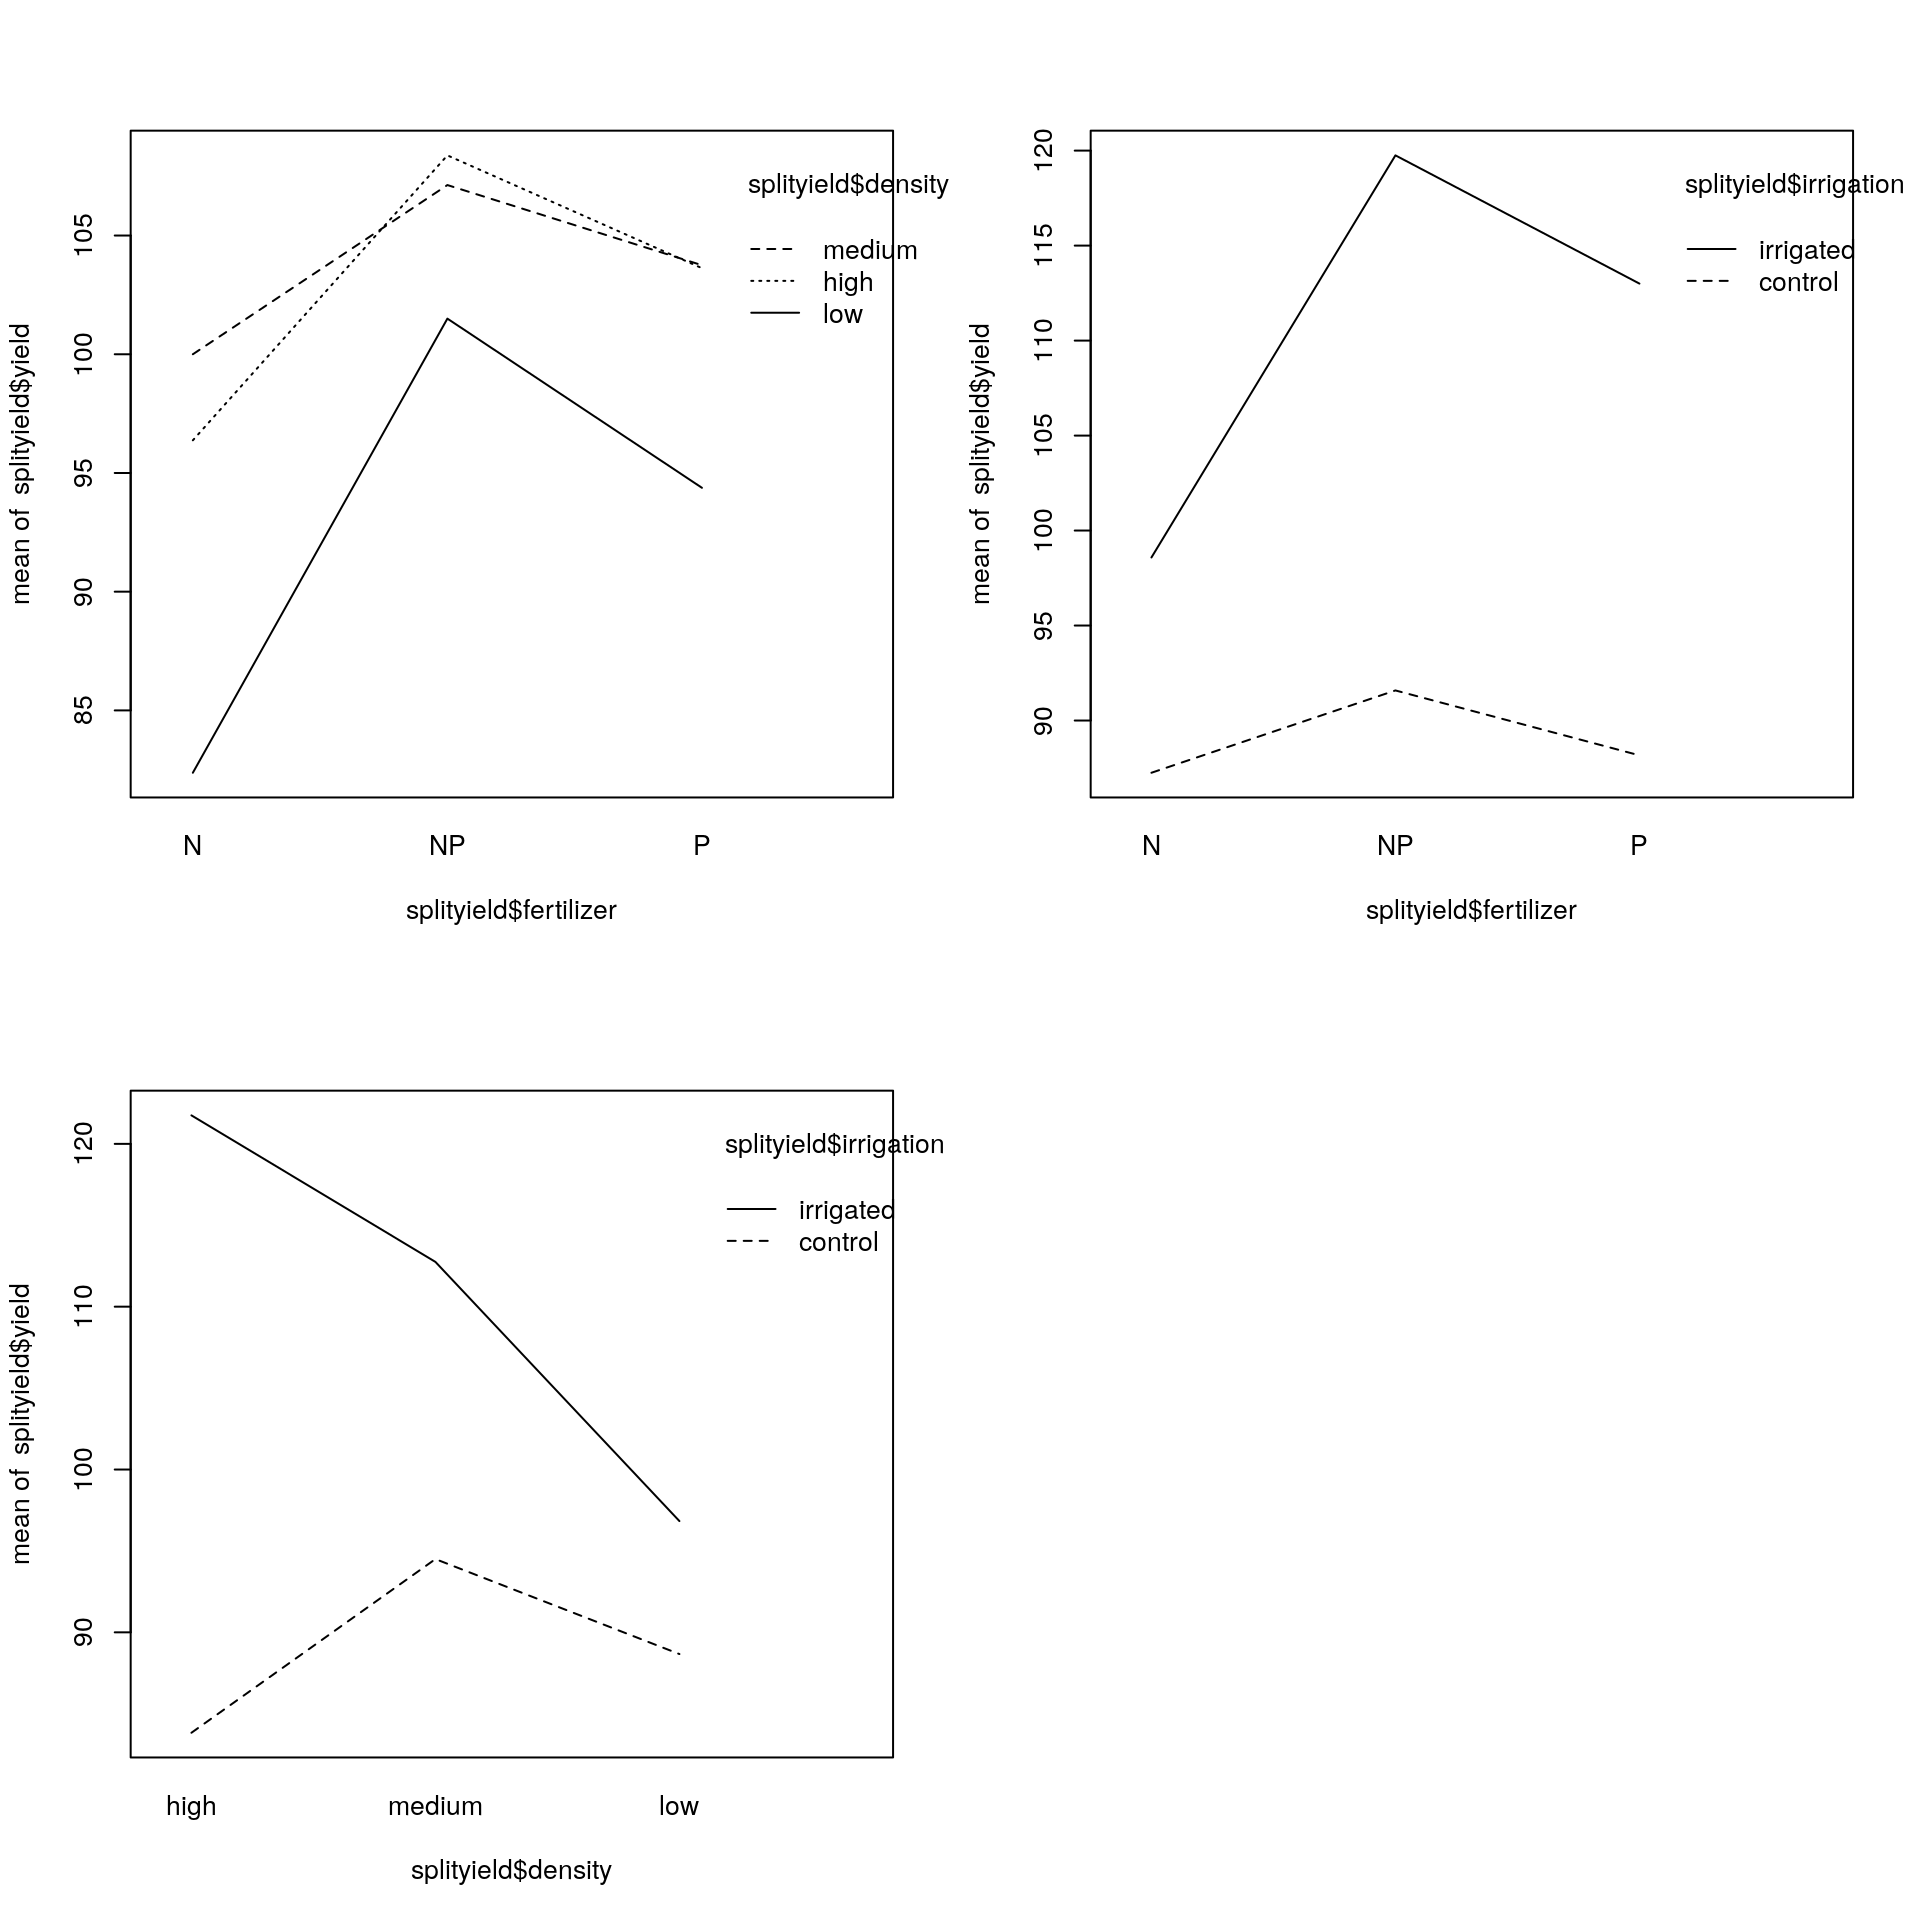
\includegraphics{_main_files/figure-latex/unnamed-chunk-163-1} \end{center}

The really pronounced interaction is that between irrigation and
density, with a reversal of the high to low density difference on the
irrigated and control plots. Overall, the 3-way interaction was not
statistically significant, nor was the 2-way interaction between density
and fertilizer. The 2-way interaction between irrigation and fertilizer,
however, was highly statistically significant.

Another way to visualise the model outputs would be to generate a plot
of the predicted yield (plus confidence intervals), for each combination
of explanatory factors. I have created a \texttt{data.frame} with these
predictions using bootstrapping. The code to replicate this can be found
\protect\hyperlink{parboot}{here}, but is a bit time consuming to run,
so I have included the predictions as a file called
\href{https://exeter-data-analytics.github.io/StatModelling/_data/split_pred.rds}{``split\_pred.rds''}.

First, read in the predictions:

\begin{Shaded}
\begin{Highlighting}[]
\NormalTok{split_pred <-}\StringTok{ }\KeywordTok{readRDS}\NormalTok{(}\StringTok{"split_pred.rds"}\NormalTok{)}
\end{Highlighting}
\end{Shaded}

Now to plot these predictions (note, once again these ease of
\texttt{ggplot2} compared to base R graphics):

\newpage

\bmp
\bblockST{\texttt{tidyverse}}

In \texttt{ggplot2} we can use the \texttt{geom\_pointrange()} function,
a \texttt{colour} aesthetic and a \texttt{facet\_wrap()}.

\eblockST
\emp
\hspace{0.01\textwidth} \bmp\bblockST{Base R}

\small

To plot the CIs in base R, we can proceed as follows:

\begin{enumerate}
\def\labelenumi{\arabic{enumi}.}
\tightlist
\item
  Set the figure layout to have two figures side-by-side.
\item
  Calculate limits for the \(y\)-axis based on the range of the CIs to
  be plotted.
\item
  Calculate manual limits for the \(x\)-axis to enable us to jitter the
  error bars around each fertiliser level.
\item
  For each level of \texttt{irrigation}:

  \begin{itemize}
  \tightlist
  \item
    Extract the subset of data corresponding to the level of
    \texttt{irrigation}.
  \item
    Produce an empty plot (setting the \(y\)-limits and \(x\)-limits).
    Remove the \(x\)-axis (using the \texttt{xaxt\ =\ "n"} argument).
    This latter step is so that we can add the \texttt{fertilizer}
    labels manually in the next step.
  \item
    For each level of \texttt{density}:

    \begin{itemize}
    \tightlist
    \item
      Extract the subset of data corresponding to the level of
      \texttt{density}.
    \item
      Sort this so that the levels of \texttt{fertilizer} are the same
      at each stage of the \texttt{i} loop\footnote{at this point,
        \texttt{temp1} will have three rows, one for each level of
        \texttt{fertilizer}}.
    \item
      Add points for the estimates and add confidence intervals using
      the \texttt{arrows()} function\footnote{I'll let you check the
        help file for \texttt{arrows()} to figure out the arguments and
        what they are doing}. Notice that I have used a \texttt{for}
      loop to allow me to plot the three CIs for each level of
      \texttt{fertilizer}. All that this loop does is to run the
      \texttt{arrows()} command 3 times, substituting \texttt{j} each
      time for the corresponding row of the sorted data set (which will
      be of length three here). You could do this explicitly in three
      lines of code if you prefer. Notice that I've jittered the points
      slightly so that the three levels of \texttt{density} can be
      plotted side-by-side.
    \end{itemize}
  \item
    Add a new \(x\)-axis and set appropriate labels for the points.
  \item
    Add a legend.
  \end{itemize}
\end{enumerate}

Phew! (Now check out the \texttt{tidyverse} solution and tell me it's
not worth the effort to learn \texttt{ggplot2}!)

\eblockST
\emp

\newpage

\bmp
\bblockST{\texttt{tidyverse}}

\small

\begin{Shaded}
\begin{Highlighting}[]
\NormalTok{## plot confidence intervals}
\KeywordTok{ggplot}\NormalTok{(newdata, }
    \KeywordTok{aes}\NormalTok{(}\DataTypeTok{x =}\NormalTok{ fertilizer, }\DataTypeTok{colour =}\NormalTok{ density)) }\OperatorTok{+}\StringTok{ }
\KeywordTok{geom_pointrange}\NormalTok{(}
    \KeywordTok{aes}\NormalTok{(}\DataTypeTok{y =}\NormalTok{ yield, }\DataTypeTok{ymin =}\NormalTok{ lci, }\DataTypeTok{ymax =}\NormalTok{ uci), }
    \DataTypeTok{position =} \KeywordTok{position_dodge}\NormalTok{(}\DataTypeTok{width =} \FloatTok{0.5}\NormalTok{)) }\OperatorTok{+}
\KeywordTok{facet_wrap}\NormalTok{(}\OperatorTok{~}\StringTok{ }\NormalTok{irrigation) }\OperatorTok{+}
\KeywordTok{labs}\NormalTok{(}\DataTypeTok{title =} \StringTok{"CIs based on fixed-effects }
\StringTok{     uncertainty ONLY"}\NormalTok{)}
\end{Highlighting}
\end{Shaded}

\begin{center}\includegraphics{_main_files/figure-latex/unnamed-chunk-246-1} \end{center}

\normalsize

\eblockST
\emp
\hspace{0.01\textwidth} \bmp\bblockST{Base R}

\scriptsize

\begin{Shaded}
\begin{Highlighting}[]
\NormalTok{## set plot layout}
\KeywordTok{par}\NormalTok{(}\DataTypeTok{mfrow =} \KeywordTok{c}\NormalTok{(}\DecValTok{1}\NormalTok{, }\DecValTok{2}\NormalTok{))}
    
\NormalTok{## set plot limits}
\NormalTok{ylims <-}\StringTok{ }\KeywordTok{min}\NormalTok{(newdata[, }\OperatorTok{-}\KeywordTok{c}\NormalTok{(}\DecValTok{1}\OperatorTok{:}\DecValTok{3}\NormalTok{)])}
\NormalTok{ylims <-}\StringTok{ }\KeywordTok{c}\NormalTok{(ylims, }\KeywordTok{max}\NormalTok{(newdata[, }\OperatorTok{-}\KeywordTok{c}\NormalTok{(}\DecValTok{1}\OperatorTok{:}\DecValTok{3}\NormalTok{)]))}
\NormalTok{xlims <-}\StringTok{ }\KeywordTok{c}\NormalTok{(}\DecValTok{0}\NormalTok{, }\FloatTok{3.5}\NormalTok{)}

\ControlFlowTok{for}\NormalTok{(m }\ControlFlowTok{in} \KeywordTok{levels}\NormalTok{(newdata}\OperatorTok{$}\NormalTok{irrigation)) \{}
\NormalTok{    ## extract control predictions}
\NormalTok{    temp <-}\StringTok{ }\NormalTok{newdata[newdata}\OperatorTok{$}\NormalTok{irrigation }\OperatorTok{==}\StringTok{ }\NormalTok{m, ]}
    
\NormalTok{    ## produce empty plot}
    \KeywordTok{plot}\NormalTok{(}\OtherTok{NULL}\NormalTok{, }\DataTypeTok{ylim =}\NormalTok{ ylims, }\DataTypeTok{xlim =}\NormalTok{ xlims, }
         \DataTypeTok{xaxt =} \StringTok{"n"}\NormalTok{, }\DataTypeTok{main =} \KeywordTok{paste}\NormalTok{(}\StringTok{"irrigation ="}\NormalTok{, m),}
         \DataTypeTok{xlab =} \StringTok{"fertilizer"}\NormalTok{, }\DataTypeTok{ylab =} \StringTok{"yield"}\NormalTok{)}
    
\NormalTok{    ## plot yield against fertiliser stratified by density}
    \ControlFlowTok{for}\NormalTok{(i }\ControlFlowTok{in} \DecValTok{1}\OperatorTok{:}\KeywordTok{length}\NormalTok{(}\KeywordTok{levels}\NormalTok{(newdata}\OperatorTok{$}\NormalTok{density))) \{}
\NormalTok{        temp1 <-}\StringTok{ }\NormalTok{temp[}
\NormalTok{            temp}\OperatorTok{$}\NormalTok{density }\OperatorTok{==}\StringTok{ }\KeywordTok{levels}\NormalTok{(newdata}\OperatorTok{$}\NormalTok{density)[i], ]}
\NormalTok{        temp1 <-}\StringTok{ }\NormalTok{temp1[}\KeywordTok{order}\NormalTok{(temp1}\OperatorTok{$}\NormalTok{fertilizer), ]}
        \ControlFlowTok{for}\NormalTok{(j }\ControlFlowTok{in} \DecValTok{1}\OperatorTok{:}\KeywordTok{nrow}\NormalTok{(temp1))\{}
            \KeywordTok{points}\NormalTok{(j }\OperatorTok{-}\StringTok{ }\FloatTok{0.2} \OperatorTok{*}\StringTok{ }\NormalTok{(}\DecValTok{2} \OperatorTok{-}\StringTok{ }\NormalTok{i), temp1}\OperatorTok{$}\NormalTok{yield[j], }
                \DataTypeTok{col =}\NormalTok{ i, }\DataTypeTok{pch =} \DecValTok{16}\NormalTok{)}
            \KeywordTok{arrows}\NormalTok{(j }\OperatorTok{-}\StringTok{ }\FloatTok{0.2} \OperatorTok{*}\StringTok{ }\NormalTok{(}\DecValTok{2} \OperatorTok{-}\StringTok{ }\NormalTok{i), temp1}\OperatorTok{$}\NormalTok{lci[j], }
\NormalTok{                j }\OperatorTok{-}\StringTok{ }\FloatTok{0.2} \OperatorTok{*}\StringTok{ }\NormalTok{(}\DecValTok{2} \OperatorTok{-}\StringTok{ }\NormalTok{i), temp1}\OperatorTok{$}\NormalTok{uci[j], }
                \DataTypeTok{length =} \FloatTok{0.1}\NormalTok{, }\DataTypeTok{col =}\NormalTok{ i, }
                \DataTypeTok{angle =} \DecValTok{90}\NormalTok{, }\DataTypeTok{code =} \DecValTok{3}\NormalTok{)}
\NormalTok{        \}}
\NormalTok{    \}}
    
\NormalTok{    ## add custom x-axis}
    \KeywordTok{axis}\NormalTok{(}\DataTypeTok{side =} \DecValTok{1}\NormalTok{, }\DataTypeTok{at =} \DecValTok{1}\OperatorTok{:}\DecValTok{3}\NormalTok{, }
         \DataTypeTok{labels =} \KeywordTok{levels}\NormalTok{(newdata}\OperatorTok{$}\NormalTok{fertilizer))}
    
\NormalTok{    ## add legend}
    \KeywordTok{legend}\NormalTok{(}\FloatTok{0.1}\NormalTok{, }
        \KeywordTok{diff}\NormalTok{(}\KeywordTok{par}\NormalTok{(}\StringTok{"usr"}\NormalTok{)[}\DecValTok{3}\OperatorTok{:}\DecValTok{4}\NormalTok{]) }\OperatorTok{*}\StringTok{ }\FloatTok{0.95} \OperatorTok{+}\StringTok{ }\KeywordTok{par}\NormalTok{(}\StringTok{"usr"}\NormalTok{)[}\DecValTok{3}\NormalTok{], }
        \DataTypeTok{legend =} \KeywordTok{levels}\NormalTok{(newdata}\OperatorTok{$}\NormalTok{density),}
        \DataTypeTok{col =} \DecValTok{1}\OperatorTok{:}\DecValTok{3}\NormalTok{, }\DataTypeTok{lty =} \DecValTok{1}\NormalTok{, }\DataTypeTok{pch =} \DecValTok{16}\NormalTok{)}
\NormalTok{\}}
\end{Highlighting}
\end{Shaded}

\begin{center}\includegraphics{_main_files/figure-latex/unnamed-chunk-247-1} \end{center}

\begin{Shaded}
\begin{Highlighting}[]
\NormalTok{## reset plot layout}
\KeywordTok{par}\NormalTok{(}\DataTypeTok{mfrow =} \KeywordTok{c}\NormalTok{(}\DecValTok{1}\NormalTok{, }\DecValTok{1}\NormalTok{))}
\end{Highlighting}
\end{Shaded}

\normalsize

\eblockST
\emp

So we can see that in the control group the \texttt{medium} density
sowing seems to produce slightly higher yields on average than the
\texttt{low} or \texttt{high} density settings, but we note that these
differences are not statistically significantly different at the 5\%
level. However, irrigation tends to not only produce higher yields on
average (except for the \texttt{N} fertiliser), but also to favour
\texttt{high} density sowing efforts, which are now much preferred over
\texttt{low} density sowing efforts (although not too dissimilar from
\texttt{medium} density efforts). The model tends to favour the
\texttt{NP} fertiliser in all cases, though there's not much between
\texttt{NP} and \texttt{P}.

\begin{quote}
\textbf{Note}: This approach does now take into account the random
effects variances or covariances. It is therefore likely to
underestimate the variance. To account for these additional
uncertainties is difficult. If you want a more consistent approach, go
\protect\hyperlink{secbayes}{Bayesian}.
\end{quote}

\section{Non-independent data: Absorbing the influence of random
effects}\label{non-independent-data-absorbing-the-influence-of-random-effects}

Eight groups of students walked through Hell's Gate National Park and
estimated the distance to groups of individuals of several species of
mammalian herbivores. Here we work with data on distances to three key
species: Thomson's gazelle, warthog and zebra. We are interested in
whether distances to these animals differ among species, whether
distances depend on animal group size, and also whether the relationship
between distance and group size differs among species. These data are
available in the
\href{https://exeter-data-analytics.github.io/StatModelling/_data/hg.rds}{``hg.rds''}
file.

A naïve analysis would ignore the identity of the student group, and
therefore treat all the distance observations as independent. It would
probably fit a \texttt{lm} of distance against species, number and the
interaction between species and number. My own exploration of the data
suggests that raw distances are skewed, and that a log-transformation
improves homoscedasticity and normality of residuals. So before
analysing we do this transformation.

\begin{Shaded}
\begin{Highlighting}[]
\NormalTok{hg <-}\StringTok{ }\KeywordTok{readRDS}\NormalTok{(}\StringTok{"hg.rds"}\NormalTok{)}
\end{Highlighting}
\end{Shaded}

\small

\begin{Shaded}
\begin{Highlighting}[]
\NormalTok{hg}\OperatorTok{$}\NormalTok{ldist <-}\StringTok{ }\KeywordTok{log}\NormalTok{(hg}\OperatorTok{$}\NormalTok{Distance)}
\NormalTok{hg_lm <-}\StringTok{ }\KeywordTok{lm}\NormalTok{(ldist }\OperatorTok{~}\StringTok{ }\NormalTok{Species }\OperatorTok{*}\StringTok{ }\NormalTok{Number, }\DataTypeTok{data =}\NormalTok{ hg)}
\KeywordTok{drop1}\NormalTok{(hg_lm, }\DataTypeTok{test =} \StringTok{"F"}\NormalTok{)}
\end{Highlighting}
\end{Shaded}

\begin{verbatim}
## Single term deletions
## 
## Model:
## ldist ~ Species * Number
##                Df Sum of Sq    RSS     AIC F value   Pr(>F)   
## <none>                      212.51 -346.77                    
## Species:Number  2    5.3917 217.91 -339.19  5.7846 0.003305 **
## ---
## Signif. codes:  0 '***' 0.001 '**' 0.01 '*' 0.05 '.' 0.1 ' ' 1
\end{verbatim}

\normalsize

This suggests a statistically significant interaction between
\texttt{Species} and \texttt{Number} (\(F_{2, 456} = 5.78\),
\(p = 0.003\)).

\small

\begin{Shaded}
\begin{Highlighting}[]
\KeywordTok{summary}\NormalTok{(hg_lm)}
\end{Highlighting}
\end{Shaded}

\begin{verbatim}
## 
## Call:
## lm(formula = ldist ~ Species * Number, data = hg)
## 
## Residuals:
##      Min       1Q   Median       3Q      Max 
## -2.32646 -0.39255  0.04353  0.44779  1.85666 
## 
## Coefficients:
##                         Estimate Std. Error t value Pr(>|t|)    
## (Intercept)            5.4357462  0.0689700  78.813  < 2e-16 ***
## Specieswarthog        -0.4178168  0.1066872  -3.916 0.000104 ***
## Specieszebra          -0.1247300  0.1203792  -1.036 0.300685    
## Number                 0.0009105  0.0118508   0.077 0.938790    
## Specieswarthog:Number  0.0156732  0.0254035   0.617 0.537563    
## Specieszebra:Number   -0.0742589  0.0238692  -3.111 0.001981 ** 
## ---
## Signif. codes:  0 '***' 0.001 '**' 0.01 '*' 0.05 '.' 0.1 ' ' 1
## 
## Residual standard error: 0.6827 on 456 degrees of freedom
## Multiple R-squared:  0.09402,    Adjusted R-squared:  0.08409 
## F-statistic: 9.465 on 5 and 456 DF,  p-value: 1.338e-08
\end{verbatim}

\normalsize

The interaction appears to be driven by a decrease in distance with
increasing group size, but only in zebras. We can draw the relevant
figure (notice that this is where \texttt{tidyverse} comes into its own,
with much more concise code resulting in a better plot).

\bmp
\bblockST{\texttt{tidyverse}}

Generate `fake' data in order to plot fitted lines:

\begin{Shaded}
\begin{Highlighting}[]
\NormalTok{newdata <-}\StringTok{ }\KeywordTok{expand.grid}\NormalTok{(}
        \DataTypeTok{Number =} \KeywordTok{seq}\NormalTok{(}\KeywordTok{min}\NormalTok{(hg}\OperatorTok{$}\NormalTok{Number), }
            \KeywordTok{max}\NormalTok{(hg}\OperatorTok{$}\NormalTok{Number), }\DataTypeTok{length =} \DecValTok{100}\NormalTok{),}
        \DataTypeTok{Species =} \KeywordTok{levels}\NormalTok{(hg}\OperatorTok{$}\NormalTok{Species)}
\NormalTok{    )}
\end{Highlighting}
\end{Shaded}

Now get the predicted values for the fake data, and back-transform
log-distance to real distances, using the \texttt{exp} command:

\begin{Shaded}
\begin{Highlighting}[]
\NormalTok{newdata <-}\StringTok{ }\NormalTok{newdata }\OperatorTok
\StringTok{    }\KeywordTok{mutate}\NormalTok{(}\DataTypeTok{Distance =} 
        \KeywordTok{exp}\NormalTok{(}\KeywordTok{predict}\NormalTok{(hg_lm, newdata)))}
\end{Highlighting}
\end{Shaded}

Now plot the fitted lines against the observed data points:

\begin{Shaded}
\begin{Highlighting}[]
\KeywordTok{ggplot}\NormalTok{(hg, }\KeywordTok{aes}\NormalTok{(}\DataTypeTok{x =}\NormalTok{ Number, }\DataTypeTok{y =}\NormalTok{ Distance, }
    \DataTypeTok{col =}\NormalTok{ Species)) }\OperatorTok{+}
\KeywordTok{geom_point}\NormalTok{() }\OperatorTok{+}\StringTok{ }
\KeywordTok{geom_line}\NormalTok{(}\DataTypeTok{data =}\NormalTok{ newdata)}
\end{Highlighting}
\end{Shaded}

\begin{center}\includegraphics{_main_files/figure-latex/unnamed-chunk-250-1} \end{center}

\eblockST
\emp
\hspace{0.01\textwidth} \bmp\bblockST{Base R}

\small

Generate `fake' data in order to plot fitted lines:

\scriptsize

\begin{Shaded}
\begin{Highlighting}[]
\NormalTok{newdata <-}\StringTok{ }\KeywordTok{expand.grid}\NormalTok{(}
    \DataTypeTok{Number =} \KeywordTok{seq}\NormalTok{(}\KeywordTok{min}\NormalTok{(hg}\OperatorTok{$}\NormalTok{Number), }\KeywordTok{max}\NormalTok{(hg}\OperatorTok{$}\NormalTok{Number), }
        \DataTypeTok{length =} \DecValTok{100}\NormalTok{),}
    \DataTypeTok{Species =} \KeywordTok{levels}\NormalTok{(hg}\OperatorTok{$}\NormalTok{Species)}
\NormalTok{)}
\end{Highlighting}
\end{Shaded}

\normalsize

Now get the predicted values for the fake data, and back-transform
log-distance to real distances, using the \texttt{exp} command:

\scriptsize

\begin{Shaded}
\begin{Highlighting}[]
\NormalTok{newdata}\OperatorTok{$}\NormalTok{Distance <-}\StringTok{ }\KeywordTok{exp}\NormalTok{(}\KeywordTok{predict}\NormalTok{(hg_lm, newdata))}
\end{Highlighting}
\end{Shaded}

\normalsize

Now plot the fitted lines against the observed data points:

\scriptsize

\begin{Shaded}
\begin{Highlighting}[]
\KeywordTok{plot}\NormalTok{(Distance }\OperatorTok{~}\StringTok{ }\NormalTok{Number, }\DataTypeTok{data =}\NormalTok{ hg, }\DataTypeTok{type =} \StringTok{"n"}\NormalTok{)}
\KeywordTok{points}\NormalTok{(Distance }\OperatorTok{~}\StringTok{ }\NormalTok{Number, }\DataTypeTok{data =}\NormalTok{ hg, }
       \DataTypeTok{subset =}\NormalTok{ (Species }\OperatorTok{==}\StringTok{ "thomsons gazelle"}\NormalTok{), }
       \DataTypeTok{pch =} \DecValTok{16}\NormalTok{)}
\KeywordTok{points}\NormalTok{(Distance }\OperatorTok{~}\StringTok{ }\NormalTok{Number, }\DataTypeTok{data =}\NormalTok{ hg, }
       \DataTypeTok{subset =}\NormalTok{ (Species }\OperatorTok{==}\StringTok{ "warthog"}\NormalTok{), }
       \DataTypeTok{pch =} \DecValTok{16}\NormalTok{,}
       \DataTypeTok{col =} \StringTok{"red"}\NormalTok{)}
\KeywordTok{points}\NormalTok{(Distance }\OperatorTok{~}\StringTok{ }\NormalTok{Number, }\DataTypeTok{data =}\NormalTok{ hg, }
       \DataTypeTok{subset =}\NormalTok{ (Species }\OperatorTok{==}\StringTok{ "zebra"}\NormalTok{), }
       \DataTypeTok{pch =} \DecValTok{16}\NormalTok{,}
       \DataTypeTok{col =} \StringTok{"blue"}\NormalTok{)}
\KeywordTok{lines}\NormalTok{(Distance }\OperatorTok{~}\StringTok{ }\NormalTok{Number, }\DataTypeTok{data =}\NormalTok{ newdata, }
      \DataTypeTok{subset =}\NormalTok{ (newdata}\OperatorTok{$}\NormalTok{Species }\OperatorTok{==}\StringTok{ "thomsons gazelle"}\NormalTok{), }
      \DataTypeTok{lwd =} \DecValTok{2}\NormalTok{)}
\KeywordTok{lines}\NormalTok{(Distance }\OperatorTok{~}\StringTok{ }\NormalTok{Number, }\DataTypeTok{data =}\NormalTok{ newdata,}
      \DataTypeTok{subset =}\NormalTok{ (newdata}\OperatorTok{$}\NormalTok{Species }\OperatorTok{==}\StringTok{ "warthog"}\NormalTok{), }
      \DataTypeTok{lwd =} \DecValTok{2}\NormalTok{, }
      \DataTypeTok{col =} \StringTok{"red"}\NormalTok{)}
\KeywordTok{lines}\NormalTok{(Distance }\OperatorTok{~}\StringTok{ }\NormalTok{Number, }\DataTypeTok{data =}\NormalTok{ newdata,}
      \DataTypeTok{subset =}\NormalTok{ (newdata}\OperatorTok{$}\NormalTok{Species }\OperatorTok{==}\StringTok{ "zebra"}\NormalTok{), }
      \DataTypeTok{lwd =} \DecValTok{2}\NormalTok{, }
      \DataTypeTok{col =} \StringTok{"blue"}\NormalTok{)}
\KeywordTok{legend}\NormalTok{(}\DecValTok{15}\NormalTok{, }\DecValTok{1000}\NormalTok{, }
       \DataTypeTok{pch =} \KeywordTok{rep}\NormalTok{(}\DecValTok{16}\NormalTok{, }\DecValTok{3}\NormalTok{), }
       \DataTypeTok{col =} \KeywordTok{c}\NormalTok{(}\StringTok{"black"}\NormalTok{, }\StringTok{"red"}\NormalTok{, }\StringTok{"blue"}\NormalTok{), }
       \DataTypeTok{legend =} \KeywordTok{c}\NormalTok{(}\StringTok{"gazelle"}\NormalTok{, }\StringTok{"warthog"}\NormalTok{, }\StringTok{"zebra"}\NormalTok{))}
\end{Highlighting}
\end{Shaded}

\begin{center}\includegraphics{_main_files/figure-latex/unnamed-chunk-253-1} \end{center}

\normalsize

\eblockST
\emp

\newpage

This naïve analysis is fundamentally flawed because the distance
estimations are not independent of each other. Several estimates come
from each of 8 student groups, and it's easy to imagine (or remember)
that observers vary dramatically in the bias of their distance estimates
(and indeed in their estimates of group size, possibly even species
identity). It's entirely possible that a group of observers who estimate
``short'' distances also encountered strangely large groups of zebras:
such a correlation between \texttt{Group.Name} and \texttt{Distance}
could drive the observed relationship for zebras.

One solution would be to fit \texttt{Group.Name} as a categorical
explanatory variable to our model. This approach has two main problems:

\begin{enumerate}
\def\labelenumi{\arabic{enumi}.}
\tightlist
\item
  It wastes valuable degrees of freedom (8 student groups, therefore 7
  d.f. as a main effect and 7 d.f. more for each interaction), giving
  the residual variance fewer d.f. and therefore weakening the power of
  our analysis.
\item
  It could easily result in a complicated minimal adequate model
  involving something that we don't really care about and which does not
  appear in our hypothesis: \texttt{Group.Name}.
\end{enumerate}

Instead we would like to be able to absorb the variance in distance
estimates among student groups. Such a model would estimate the
relationship between \texttt{Distance}, \texttt{Species} and
\texttt{Number} for an \textbf{average} group of observers. It could
also tell us just how much variance exists among groups of observers.

This is a classic example of where a \textbf{mixed-effects model} is
useful. We care about the influence of \texttt{Species} and
\texttt{Number} on \texttt{Distance}. These are \textbf{fixed effects}.
We know that \texttt{Group.Name} will have an influence on
\texttt{Distance}, but the categories of \texttt{Group.Name} are
uninformative to the lay reader and cannot be replicated in future field
trips. Hence we treat \texttt{Group.Name} as a \textbf{random effect}.
An ideal mixed-effects model will test the influence of \texttt{Species}
and \texttt{Number} on \texttt{Distance}, meanwhile absorbing the
influence of \texttt{Group.Name}.

\begin{Shaded}
\begin{Highlighting}[]
\NormalTok{hg_lmer <-}\StringTok{ }\KeywordTok{lmer}\NormalTok{(ldist }\OperatorTok{~}\StringTok{ }\NormalTok{Species }\OperatorTok{*}\StringTok{ }\NormalTok{Number }\OperatorTok{+}\StringTok{ }\NormalTok{(}\DecValTok{1} \OperatorTok{|}\StringTok{ }\NormalTok{Group.Name), }\DataTypeTok{data =}\NormalTok{ hg)}
\end{Highlighting}
\end{Shaded}

Note that there is no nesting going on here; \texttt{Species} and
\texttt{Number} have the same interpretation regardless of the
\texttt{Group.Name}. Let's take a look at the summary of the fitted
model.

\begin{Shaded}
\begin{Highlighting}[]
\KeywordTok{summary}\NormalTok{(hg_lmer)}
\end{Highlighting}
\end{Shaded}

\begin{verbatim}
## Linear mixed model fit by REML ['lmerMod']
## Formula: ldist ~ Species * Number + (1 | Group.Name)
##    Data: hg
## 
## REML criterion at convergence: 814.2
## 
## Scaled residuals: 
##     Min      1Q  Median      3Q     Max 
## -4.4891 -0.6386 -0.0128  0.5896  2.6806 
## 
## Random effects:
##  Groups     Name        Variance Std.Dev.
##  Group.Name (Intercept) 0.2085   0.4566  
##  Residual               0.3046   0.5519  
## Number of obs: 462, groups:  Group.Name, 8
## 
## Fixed effects:
##                         Estimate Std. Error t value
## (Intercept)            5.4411458  0.1721299  31.611
## Specieswarthog        -0.3947870  0.0869880  -4.538
## Specieszebra          -0.2975063  0.0997439  -2.983
## Number                -0.0001202  0.0099875  -0.012
## Specieswarthog:Number -0.0049066  0.0208474  -0.235
## Specieszebra:Number   -0.0289725  0.0199376  -1.453
## 
## Correlation of Fixed Effects:
##             (Intr) Spcswr Spcszb Number Spcsw:N
## Speciswrthg -0.216                             
## Specieszebr -0.173  0.362                      
## Number      -0.235  0.415  0.318               
## Spcswrthg:N  0.101 -0.710 -0.148 -0.460        
## Spcszbr:Nmb  0.084 -0.196 -0.747 -0.416  0.200
\end{verbatim}

This summary table is packed with information. First, we can see that
the standard deviation in \texttt{Distance} among student groups is
0.46, which is almost as big as the residual standard deviation of 0.55.
This suggests variation among observers is important and could
dramatically change our results. Second, the estimates of slopes and
differences between species are going in the `same direction' as the
estimates from the naïve \texttt{lm()} analysis, but seem to be smaller.

With \textbf{unbalanced} experimental designs like this, the fixed
effects part of the model cannot be simplified in the usual way. This is
because the removal of a fixed effect will \textbf{fundamentally} change
the model fit: it's not just a case of dumping the deviance explained by
a fixed effect into the residual deviance, because the residual deviance
is different for each nested level of the experimental design.
Furthermore, if the experiment is unbalanced, we should beware of using
F-tests to check the statistical significance of terms. Instead, we
should use AIC or \textbf{likelihood ratio tests}, and if we do this we
need to change the fitting mechanism from REML to ML whilst performing
LRT. (We do this \emph{in situ} using the \texttt{update()} function.)

\begin{Shaded}
\begin{Highlighting}[]
\KeywordTok{drop1}\NormalTok{(}\KeywordTok{update}\NormalTok{(hg_lmer, }\DataTypeTok{REML =}\NormalTok{ F), }\DataTypeTok{test =} \StringTok{"Chisq"}\NormalTok{)}
\end{Highlighting}
\end{Shaded}

\begin{verbatim}
## Single term deletions
## 
## Model:
## ldist ~ Species * Number + (1 | Group.Name)
##                Df    AIC    LRT Pr(Chi)
## <none>            800.99               
## Species:Number  2 799.15 2.1605  0.3395
\end{verbatim}

As usual, likelihood ratio tests in this context have a chi-squared
distribution with d.f. equal to the difference in d.f. between the
models. Here we have 8 - 6 = 2 d.f. So, here we find no evidence for an
interaction between \texttt{Species} and \texttt{Number}
(\(X^2_2 = 2.16\), \(p = 0.34\)).

Since we have an \textbf{unbalanced} design here, we can continue model
simplification by dropping each of the main effect terms from the
current model and seeing which has the largest impact on model fit (in
this case the model simplification will be different depending on the
\textbf{\emph{order}} in which variables are added/removed from the
model).

\small

\begin{Shaded}
\begin{Highlighting}[]
\NormalTok{## set baseline model from previous round}
\NormalTok{hg_lmer <-}\StringTok{ }\KeywordTok{update}\NormalTok{(hg_lmer, }\OperatorTok{~}\StringTok{ }\NormalTok{. }\OperatorTok{-}\StringTok{ }\NormalTok{Species}\OperatorTok{:}\NormalTok{Number)}

\NormalTok{## now drop terms compare to baseline model}
\KeywordTok{drop1}\NormalTok{(}\KeywordTok{update}\NormalTok{(hg_lmer, }\DataTypeTok{REML =}\NormalTok{ F), }\DataTypeTok{test =} \StringTok{"Chisq"}\NormalTok{)}
\end{Highlighting}
\end{Shaded}

\begin{verbatim}
## Single term deletions
## 
## Model:
## ldist ~ Species + Number + (1 | Group.Name)
##         Df    AIC    LRT   Pr(Chi)    
## <none>     799.15                     
## Species  2 849.64 54.490 1.471e-12 ***
## Number   1 797.68  0.528    0.4674    
## ---
## Signif. codes:  0 '***' 0.001 '**' 0.01 '*' 0.05 '.' 0.1 ' ' 1
\end{verbatim}

\normalsize

Here dropping \texttt{Number} has little impact on the model fit,
whereas dropping \texttt{Species} results in a statistically
significantly inferior fit. Hence the next stage is to drop
\texttt{Number}. Therefore our baseline model now has just the main
effect for \texttt{Species}. The final stage is to drop \texttt{Species}
and assess the change in fit relative to our current model.

\hypertarget{tsk22}{}\bblockT[Question]{\phantomsection\label{sol22}22}

Why do we need to do this last step, since we assessed the impact of
removing \texttt{Species} before? \eblockT

\hyperlink{sol22}{\buttonS{Show Answer on P\colpageref{tsk22}}}

\begin{Shaded}
\begin{Highlighting}[]
\NormalTok{## set baseline model from previous round}
\NormalTok{hg_lmer <-}\StringTok{ }\KeywordTok{update}\NormalTok{(hg_lmer, }\OperatorTok{~}\StringTok{ }\NormalTok{. }\OperatorTok{-}\StringTok{ }\NormalTok{Number)}

\NormalTok{## now drop terms compare to baseline model}
\KeywordTok{drop1}\NormalTok{(}\KeywordTok{update}\NormalTok{(hg_lmer, }\DataTypeTok{REML =}\NormalTok{ F), }\DataTypeTok{test =} \StringTok{"Chisq"}\NormalTok{)}
\end{Highlighting}
\end{Shaded}

\begin{verbatim}
## Single term deletions
## 
## Model:
## ldist ~ Species + (1 | Group.Name)
##         Df    AIC    LRT   Pr(Chi)    
## <none>     797.68                     
## Species  2 847.64 53.965 1.913e-12 ***
## ---
## Signif. codes:  0 '***' 0.001 '**' 0.01 '*' 0.05 '.' 0.1 ' ' 1
\end{verbatim}

This suggests there is a clear effect of \texttt{Species} identity on
\texttt{log(Distance)} (\(X^2_2 = 54.0\), \(p < 0.001\)).

Now we'd like to see our model summary (notice that R has automatically
kept the REML fit; since we only converted the model objects to use ML
during the model comparison exercise):

\begin{Shaded}
\begin{Highlighting}[]
\KeywordTok{summary}\NormalTok{(hg_lmer)}
\end{Highlighting}
\end{Shaded}

\scriptsize

\begin{verbatim}
## Linear mixed model fit by REML ['lmerMod']
## Formula: ldist ~ Species + (1 | Group.Name)
##    Data: hg
## 
## REML criterion at convergence: 797.1
## 
## Scaled residuals: 
##     Min      1Q  Median      3Q     Max 
## -4.4743 -0.6479 -0.0538  0.5904  2.6838 
## 
## Random effects:
##  Groups     Name        Variance Std.Dev.
##  Group.Name (Intercept) 0.2161   0.4649  
##  Residual               0.3042   0.5516  
## Number of obs: 462, groups:  Group.Name, 8
## 
## Fixed effects:
##                Estimate Std. Error t value
## (Intercept)     5.43619    0.17008  31.962
## Specieswarthog -0.41088    0.06060  -6.780
## Specieszebra   -0.40508    0.06627  -6.113
## 
## Correlation of Fixed Effects:
##             (Intr) Spcswr
## Speciswrthg -0.179       
## Specieszebr -0.164  0.466
\end{verbatim}

\normalsize

This final summary tells us that the standard deviation among observer
groups is almost as big as the residual standard deviation in distances.
It tells us that both warthogs and zebra are closer to the observer than
Thomson's gazelles, which are approximately \(e^{5.44} = 230\) metres
away on average. The number of animals in a group has negligible
influence on distance given the uncertainties in the data.

We're now left with a final model that has a single categorical
variable. We could provide a boxplot of the raw data to describe it, but
in this instance it would be misleading because it would not
differentiate between observer-level noise and residual noise. In this
instance we will produce confidence intervals for the mean distance from
the road for each species and plot them.

The simplest way to generate confidence intervals for each of the three
parameters of the model is to refit the model three times, changing the
baseline species each time and using the \texttt{confint} function to
extract the confidence intervals (converting to the correct scale at the
end). For consistency we'll use a bootstrap method to generate the
intervals (using 500 replicates, which is the default, though you might
want to change to a larger number in practice). (Note that you could use
a \texttt{predict()} solution as in the
\protect\hyperlink{parboot}{earlier example}, which is often easier for
more complex predictions.)

\begin{Shaded}
\begin{Highlighting}[]
\NormalTok{hg_cis <-}\StringTok{ }\KeywordTok{matrix}\NormalTok{(}\OtherTok{NA}\NormalTok{, }\KeywordTok{length}\NormalTok{(}\KeywordTok{levels}\NormalTok{(hg}\OperatorTok{$}\NormalTok{Species)), }\DecValTok{3}\NormalTok{)}
\NormalTok{hg_spec <-}\StringTok{ }\KeywordTok{levels}\NormalTok{(hg}\OperatorTok{$}\NormalTok{Species)}
\ControlFlowTok{for}\NormalTok{(i }\ControlFlowTok{in} \DecValTok{1}\OperatorTok{:}\KeywordTok{length}\NormalTok{(hg_spec))\{}
\NormalTok{    hg}\OperatorTok{$}\NormalTok{Species <-}\StringTok{ }\KeywordTok{relevel}\NormalTok{(hg}\OperatorTok{$}\NormalTok{Species, }\DataTypeTok{ref =} \KeywordTok{levels}\NormalTok{(hg}\OperatorTok{$}\NormalTok{Species)[i])}
\NormalTok{    hg_lmer <-}\StringTok{ }\KeywordTok{update}\NormalTok{(hg_lmer, }\DataTypeTok{data =}\NormalTok{ hg)}
\NormalTok{    hg_cis[i, ] <-}\StringTok{ }\KeywordTok{c}\NormalTok{(}
        \KeywordTok{coef}\NormalTok{(}\KeywordTok{summary}\NormalTok{(hg_lmer))[ , }\StringTok{"Estimate"}\NormalTok{][}\DecValTok{1}\NormalTok{], }
        \KeywordTok{confint}\NormalTok{(hg_lmer, }\DataTypeTok{quiet =}\NormalTok{ T, }\DataTypeTok{method =} \StringTok{"boot"}\NormalTok{)[}\DecValTok{3}\NormalTok{, ]}
\NormalTok{    )}
\NormalTok{\}}
\NormalTok{hg_cis <-}\StringTok{ }\KeywordTok{exp}\NormalTok{(hg_cis)}
\NormalTok{hg_cis <-}\StringTok{ }\KeywordTok{as.data.frame}\NormalTok{(hg_cis)}
\KeywordTok{colnames}\NormalTok{(hg_cis) <-}\StringTok{ }\KeywordTok{c}\NormalTok{(}\StringTok{"mean"}\NormalTok{, }\StringTok{"lci"}\NormalTok{, }\StringTok{"uci"}\NormalTok{)}
\NormalTok{hg_cis}\OperatorTok{$}\NormalTok{Species <-}\StringTok{ }\NormalTok{hg_spec}
\NormalTok{hg_cis}
\end{Highlighting}
\end{Shaded}

\begin{verbatim}
##       mean      lci      uci          Species
## 1 229.5666 169.8597 327.1454 thomsons gazelle
## 2 152.2176 111.4347 213.6262          warthog
## 3 153.1030 107.7038 211.2413            zebra
\end{verbatim}

\newpage

\bmp
\bblockST{\texttt{tidyverse}}

In \texttt{ggplot2} we can use the \texttt{geom\_pointrange()} function.

\small

\begin{Shaded}
\begin{Highlighting}[]
\KeywordTok{ggplot}\NormalTok{(hg_cis, }\KeywordTok{aes}\NormalTok{(}\DataTypeTok{x =}\NormalTok{ Species)) }\OperatorTok{+}
\StringTok{    }\KeywordTok{geom_pointrange}\NormalTok{(}
        \KeywordTok{aes}\NormalTok{(}\DataTypeTok{y =}\NormalTok{ mean, }\DataTypeTok{ymin =}\NormalTok{ lci, }
        \DataTypeTok{ymax =}\NormalTok{ uci)) }\OperatorTok{+}
\StringTok{    }\KeywordTok{xlab}\NormalTok{(}\StringTok{"Species"}\NormalTok{) }\OperatorTok{+}\StringTok{ }
\StringTok{    }\KeywordTok{ylab}\NormalTok{(}\StringTok{"Distance from road (m)"}\NormalTok{)}
\end{Highlighting}
\end{Shaded}

\begin{center}\includegraphics{_main_files/figure-latex/unnamed-chunk-254-1} \end{center}

\normalsize

\eblockST
\emp
\hspace{0.01\textwidth} \bmp\bblockST{Base R}

To plot the CIs in base R, we can proceed as follows:

\begin{enumerate}
\def\labelenumi{\arabic{enumi}.}
\tightlist
\item
  Calculate limits for the \(y\)-axis based on the range of the CIs to
  be plotted.
\item
  Calculate manual limits for the \(x\)-axis to enable the species names
  to render correctly.
\item
  Produce a scatterplot of points defined on the ranges set above, but
  remove the \(x\)-axis (using the \texttt{xaxt\ =\ "n"} argument). This
  latter step is so that we can add the species labels manually in the
  next step.
\item
  Add a new \(x\)-axis and set appropriate labels for the points.
\item
  Add confidence intervals using the \texttt{arrows()} function. Notice
  that Ive used a \texttt{for} loop to allow me to plot the three CIs in
  one line of code as in the earlier example. You could do this
  explicitly in three lines of code if you prefer.
\end{enumerate}

\small

\begin{Shaded}
\begin{Highlighting}[]
\NormalTok{ylims <-}\StringTok{ }\KeywordTok{c}\NormalTok{(}\DecValTok{0}\NormalTok{, }\KeywordTok{max}\NormalTok{(hg_cis[, }\OperatorTok{-}\KeywordTok{ncol}\NormalTok{(hg_cis)]))}
\NormalTok{xlims <-}\StringTok{ }\KeywordTok{c}\NormalTok{(}\FloatTok{0.5}\NormalTok{, }\FloatTok{3.5}\NormalTok{)}
\KeywordTok{plot}\NormalTok{(}\DecValTok{1}\OperatorTok{:}\KeywordTok{nrow}\NormalTok{(hg_cis), hg_cis}\OperatorTok{$}\NormalTok{mean, }
     \DataTypeTok{xlab =} \StringTok{"Species"}\NormalTok{, }
     \DataTypeTok{ylab =} \StringTok{"Distance from road (m)"}\NormalTok{, }
     \DataTypeTok{xaxt =} \StringTok{"n"}\NormalTok{, }\DataTypeTok{pch =} \DecValTok{16}\NormalTok{, }\DataTypeTok{ylim =}\NormalTok{ ylims, }
     \DataTypeTok{xlim =}\NormalTok{ xlims)}
\KeywordTok{axis}\NormalTok{(}\DecValTok{1}\NormalTok{, }\DecValTok{1}\OperatorTok{:}\KeywordTok{nrow}\NormalTok{(hg_cis), hg_cis}\OperatorTok{$}\NormalTok{Species)}
\ControlFlowTok{for}\NormalTok{(i }\ControlFlowTok{in} \DecValTok{1}\OperatorTok{:}\KeywordTok{nrow}\NormalTok{(hg_cis)) \{}
    \KeywordTok{arrows}\NormalTok{(i, hg_cis}\OperatorTok{$}\NormalTok{lci[i], }
\NormalTok{           i, hg_cis}\OperatorTok{$}\NormalTok{uci[i], }
           \DataTypeTok{code =} \DecValTok{3}\NormalTok{, }
           \DataTypeTok{angle =} \DecValTok{90}\NormalTok{, }
           \DataTypeTok{length =} \FloatTok{0.1}\NormalTok{)}
\NormalTok{\}}
\end{Highlighting}
\end{Shaded}

\begin{center}\includegraphics{_main_files/figure-latex/unnamed-chunk-255-1} \end{center}

\normalsize

\eblockST
\emp

\section{Model checking with mixed
models}\label{model-checking-with-mixed-models}

We need to be just as conscious of testing the assumptions of mixed
effects models as we are with any other. The assumptions are:

\begin{enumerate}
\def\labelenumi{\arabic{enumi}.}
\tightlist
\item
  Within-group errors are independent and normally distributed with mean
  zero and variance \(\sigma^2\).
\item
  Within-group errors are independent of the random effects.
\item
  Random effects are normally distributed with mean zero.
\item
  Random effects have a covariance matrix \(\Psi\) that does not depend
  on the group\ldots{} this is rather advanced.
\item
  Random effects are independent for different groups, except as
  specified by nesting\ldots{} I'm not really sure what this means.
\end{enumerate}

Several model check plots would help us to confirm/deny these
assumptions, but note that QQ-plots may not be relevant because of the
model structure. Two commonly-used plots are:

\begin{enumerate}
\def\labelenumi{\arabic{enumi}.}
\tightlist
\item
  A simple plot of residuals against fitted values, irrespective of
  random effects (note we have to do this ``by hand'' here):
\end{enumerate}

\begin{Shaded}
\begin{Highlighting}[]
\KeywordTok{plot}\NormalTok{(}\KeywordTok{resid}\NormalTok{(hg_lmer) }\OperatorTok{~}\StringTok{ }\KeywordTok{fitted}\NormalTok{(hg_lmer))}
\end{Highlighting}
\end{Shaded}

\begin{center}\includegraphics{_main_files/figure-latex/unnamed-chunk-183-1} \end{center}

It can often be useful to check the distribution of residuals in each of
the groups (e.g.~blocks) to check assumptions 1 and 2. We can do this by
plotting the residuals against the fitted values, separately for each
level of the random effect, using the precious \texttt{coplot} function:

\begin{Shaded}
\begin{Highlighting}[]
\KeywordTok{coplot}\NormalTok{(}\KeywordTok{resid}\NormalTok{(hg_lmer) }\OperatorTok{~}\StringTok{ }\KeywordTok{fitted}\NormalTok{(hg_lmer) }\OperatorTok{|}\StringTok{ }\NormalTok{hg}\OperatorTok{$}\NormalTok{Group.Name)}
\end{Highlighting}
\end{Shaded}

\begin{center}\includegraphics{_main_files/figure-latex/unnamed-chunk-184-1} \end{center}

You'll notice that each sub-figure of this plot, which refers to an
individual group of observers, doesn't contain much data. Therefore it's
hard to judge whether the spread of residuals around fitted values is
the same for each observer group. But, with better-replicated
experiments (i.e.~with many more animals seen per observer group) we
could check that the residuals are homoscedastic both \textbf{within}
and \textbf{among} observers. (Note that the order of the coplots
relating to the groups denoted in the top plot is left-to-right,
bottom-to-top: so \texttt{bilbo\textquotesingle{}s\ badgers} are
bottom-left, \texttt{Mega-my-fauna} are bottom-middle and so on\ldots{})

\section{Why aren't GLMs much good at modelling non-independent
data?}\label{why-arent-glms-much-good-at-modelling-non-independent-data}

This is a short section, but very important. When you perform ANOVA or
linear regression with a Gaussian (normal) error structure, you can use
F-tests which are based on `model' and `residual' mean-squares or
deviances (remember an F-statistic is the ratio of two variances). When
data are non-independent, this is really useful because you can choose
which part of the experimental design structure from which to select
your residual deviance. Remember that you can also use likelihood ratio
testing, in which case the chi-squared test statistic is an
\textbf{exact} test (although subtlely different to the F-test).

When you perform Generalised Linear Modelling with non-normal error
structures, you have to use likelihood ratio testing (i.e.~chi-square
tests). In the case of a standard GLM, then the LRT test statistic is
\textbf{asymptotically chi-squared} (i.e.~it's approximately
chi-squared, where the approximation gets better as the sample size gets
bigger). However, these are based only on `model' deviance and do not
take into account residual deviance. Hence a model of non-independent
data cannot provide correct chi-square tests because they ignore the
nesting in the experimental design.

\begin{quote}
\textbf{Moral}: It's far better to use \textbf{Generalised Linear Mixed
Modelling} in these cases.
\end{quote}

\section{Generalised Linear Mixed Modelling
(GLMM)}\label{generalised-linear-mixed-modelling-glmm}

Obviously given your expertise with non-normal data and error
structures, by now (if you're still reading) you'll be craving a
mixed-effects modelling technique that copes with Poisson, binomial,
quasi etc. errors: \texttt{glmer()} gives it a good try.

As an example, suppose our hypotheses change. Now we believe that the
group sizes vary among species and with distance from the road. Using
\texttt{Number} as a response variable is unlikely to have normal
residuals (I'm confident). If this was a GLM, we would start by trying
\texttt{family\ =\ poisson}, because the data are counts (close to
zero). Miraculously, that's all we have to do in \texttt{glmer()} as
well.

\begin{Shaded}
\begin{Highlighting}[]
\NormalTok{hometime <-}\StringTok{ }\KeywordTok{glmer}\NormalTok{(Number }\OperatorTok{~}\StringTok{ }\NormalTok{Species }\OperatorTok{*}\StringTok{ }\NormalTok{ldist }\OperatorTok{+}\StringTok{ }\NormalTok{(}\DecValTok{1} \OperatorTok{|}\StringTok{ }\NormalTok{Group.Name), }
    \DataTypeTok{data =}\NormalTok{ hg, }\DataTypeTok{family =}\NormalTok{ poisson)}
\KeywordTok{summary}\NormalTok{(hometime)}
\end{Highlighting}
\end{Shaded}

\newpage

\begin{verbatim}
## Generalized linear mixed model fit by maximum likelihood (Laplace
##   Approximation) [glmerMod]
##  Family: poisson  ( log )
## Formula: Number ~ Species * ldist + (1 | Group.Name)
##    Data: hg
## 
##      AIC      BIC   logLik deviance df.resid 
##   2241.8   2270.8  -1113.9   2227.8      455 
## 
## Scaled residuals: 
##     Min      1Q  Median      3Q     Max 
## -1.9259 -0.9735 -0.4698  0.5877  9.6966 
## 
## Random effects:
##  Groups     Name        Variance Std.Dev.
##  Group.Name (Intercept) 0.128    0.3577  
## Number of obs: 462, groups:  Group.Name, 8
## 
## Fixed effects:
##                               Estimate Std. Error z value Pr(>|z|)    
## (Intercept)                    2.50760    0.34501   7.268 3.64e-13 ***
## Specieswarthog                -1.84315    0.43850  -4.203 2.63e-05 ***
## Speciesthomsons gazelle       -1.11766    0.45641  -2.449 0.014332 *  
## ldist                         -0.23485    0.06493  -3.617 0.000298 ***
## Specieswarthog:ldist           0.32048    0.08687   3.689 0.000225 ***
## Speciesthomsons gazelle:ldist  0.23311    0.08697   2.680 0.007354 ** 
## ---
## Signif. codes:  0 '***' 0.001 '**' 0.01 '*' 0.05 '.' 0.1 ' ' 1
## 
## Correlation of Fixed Effects:
##             (Intr) Spcswr Spcstg ldist  Spcsw:
## Speciswrthg -0.571                            
## Spcsthmsnsg -0.502  0.413                     
## ldist       -0.920  0.607  0.533              
## Spcswrthg:l  0.576 -0.988 -0.417 -0.629       
## Spcsthgzll:  0.541 -0.435 -0.989 -0.591  0.451
\end{verbatim}

Simplification to find the Minimal Adequate Model is\ldots{} a challenge
for you to complete!

Congratulations.

\hypertarget{parboot}{\section{Parametric bootstrapping}\label{parboot}}

Bootstrapping is a resampling technique that was designed for inference
when it is not possible (or hard) to generate theoretical sampling
distributions for particular quantities of interest. It was introduced
by \href{https://en.wikipedia.org/wiki/Bradley_Efron}{Bradley Efron} in
1979. The name is based on the adage: ``to pull oneself up by one's
bootstraps''.

The basic idea is that we can generate \textbf{empirical} sampling
distributions for a quantity of interest (e.g.~a median for example) by
sampling from the underlying system a very large number of times and
calculating the quantity in each case. This sampling distribution can be
used directly to generate confidence intervals for example. Of course,
in practice we cannot sample multiple times from the underlying system
(we often only have one replicate---the \textbf{observed data}).
Instead, bootstrapping aims to approximate this idea by instead
\textbf{re-sampling with replacement} from the observed data, and then
generating empirical bootstrapped sampling distributions. These ideas
have been developed greatly over the years, but the technique is
attractive because it is simple to implement (although the estimates are
often slightly biased). \texttt{lme4} has a function \texttt{bootMer()}
that can be used to implement specific types of bootstrapping---in this
case we want to use \textbf{parametric} bootstrapping. We do not dwell
on the details here, but if you want more information please come and
see me.

To generate the confidence intervals used in the
\protect\hyperlink{secsplit}{split-plot} design
\protect\hyperlink{splitplot}{earlier}, you can use the following code:

\begin{Shaded}
\begin{Highlighting}[]
\NormalTok{## new data to predict to}
\NormalTok{newdata <-}\StringTok{ }\KeywordTok{expand.grid}\NormalTok{(}
    \DataTypeTok{density =} \KeywordTok{levels}\NormalTok{(splityield}\OperatorTok{$}\NormalTok{density),}
    \DataTypeTok{irrigation =} \KeywordTok{levels}\NormalTok{(splityield}\OperatorTok{$}\NormalTok{irrigation),}
    \DataTypeTok{fertilizer =} \KeywordTok{levels}\NormalTok{(splityield}\OperatorTok{$}\NormalTok{fertilizer)}
\NormalTok{)}

\NormalTok{## prediction function to use in bootstrap routine}
\NormalTok{predFun <-}\StringTok{ }\ControlFlowTok{function}\NormalTok{(mod) \{}
  \KeywordTok{predict}\NormalTok{(mod, }\DataTypeTok{newdata =}\NormalTok{ newdata, }\DataTypeTok{re.form =} \OtherTok{NA}\NormalTok{)}
\NormalTok{\}}

\NormalTok{## produce 1000 bootstrapped samples}
\NormalTok{boot1 <-}\StringTok{ }\KeywordTok{bootMer}\NormalTok{(split_lmer, predFun, }\DataTypeTok{nsim =} \DecValTok{1000}\NormalTok{, }\DataTypeTok{type =} \StringTok{"parametric"}\NormalTok{, }\DataTypeTok{re.form =} \OtherTok{NA}\NormalTok{)}

\NormalTok{## function to produce percentile based CIs}
\NormalTok{sumBoot <-}\StringTok{ }\ControlFlowTok{function}\NormalTok{(merBoot) \{}
    \KeywordTok{data.frame}\NormalTok{(}
        \DataTypeTok{yield =} \KeywordTok{apply}\NormalTok{(merBoot}\OperatorTok{$}\NormalTok{t, }\DecValTok{2}\NormalTok{, }\ControlFlowTok{function}\NormalTok{(x)\{}
            \KeywordTok{mean}\NormalTok{(x, }\DataTypeTok{na.rm =}\NormalTok{ T)}
\NormalTok{        \}),}
        \DataTypeTok{lci =} \KeywordTok{apply}\NormalTok{(merBoot}\OperatorTok{$}\NormalTok{t, }\DecValTok{2}\NormalTok{, }\ControlFlowTok{function}\NormalTok{(x)\{}
            \KeywordTok{quantile}\NormalTok{(x, }\DataTypeTok{probs =} \FloatTok{0.025}\NormalTok{, }\DataTypeTok{na.rm =}\NormalTok{ T)}
\NormalTok{        \}),}
        \DataTypeTok{uci =} \KeywordTok{apply}\NormalTok{(merBoot}\OperatorTok{$}\NormalTok{t, }\DecValTok{2}\NormalTok{, }\ControlFlowTok{function}\NormalTok{(x)\{}
            \KeywordTok{quantile}\NormalTok{(x, }\DataTypeTok{probs =} \FloatTok{0.975}\NormalTok{, }\DataTypeTok{na.rm =}\NormalTok{ T)}
\NormalTok{        \})}
\NormalTok{    )}
\NormalTok{\}}

\NormalTok{## bind CIs to newdata}
\NormalTok{split_pred <-}\StringTok{ }\KeywordTok{cbind}\NormalTok{(newdata, }\KeywordTok{sumBoot}\NormalTok{(boot1))}
\end{Highlighting}
\end{Shaded}

\hypertarget{secbayes}{\section{Bayesian modelling}\label{secbayes}}

Many of the challenges associated with \textbf{mixed effects} models go
away if you move your inference into a \textbf{Bayesian} framework.
That's not to say that other challenges do not arise in their place,
mainly in terms of variable selection, however, in general I would
recommend using a Bayesian framework for complex models with
hierarchical structures, particularly spatio-temporal modelling.

For GLMMs there is an R package called
\href{https://cran.r-project.org/web/packages/MCMCglmm/index.html}{\texttt{MCMCglmm}}
that will fit a wide range of models in a Bayesian framework.
Alternatively there are general purpose Bayesian packages such as
\href{https://www.mrc-bsu.cam.ac.uk/software/bugs/the-bugs-project-winbugs/}{WinBUGS},
\href{http://www.openbugs.net/w/FrontPage}{OpenBUGS},
\href{http://mcmc-jags.sourceforge.net/}{JAGS} or more recently
\href{http://mc-stan.org/}{Stan}.

These approaches are beyond the scope of this course, but we are hoping
to run a Bayesian Modelling workshop next year, so keep your ears to the
ground!

\newgeometry{margin=0.5in}

\appendix


\chapter{Answers}\label{answers}

\hypertarget{sol1}{} \bblockS[Solution]{\phantomsection\label{tsk1}1}
\bmp
\bblockST{Base R}

\begin{Shaded}
\begin{Highlighting}[]
\KeywordTok{plot}\NormalTok{(longevity }\OperatorTok{~}\StringTok{ }\NormalTok{thorax, }\DataTypeTok{data =}\NormalTok{ ff, }
     \DataTypeTok{pch=}\DecValTok{19}\NormalTok{, }\DataTypeTok{col=}\StringTok{'darkgrey'}\NormalTok{)}
\end{Highlighting}
\end{Shaded}

\begin{center}\includegraphics[width=0.6\linewidth]{_main_files/figure-latex/unnamed-chunk-190-1} \end{center}

The plot suggests that a linear relationship might exist between the two
variables. So we can proceed by fitting a linear model in R.

\eblockST
\emp
\hspace{0.01\textwidth} \bmp\bblockST{\texttt{tidyverse}}

\begin{Shaded}
\begin{Highlighting}[]
\KeywordTok{ggplot}\NormalTok{(ff) }\OperatorTok{+}
\StringTok{    }\KeywordTok{geom_point}\NormalTok{(}\KeywordTok{aes}\NormalTok{(}\DataTypeTok{x =}\NormalTok{ thorax, }\DataTypeTok{y =}\NormalTok{ longevity))}
\end{Highlighting}
\end{Shaded}

\begin{center}\includegraphics{_main_files/figure-latex/unnamed-chunk-191-1} \end{center}

The plot suggests that a linear relationship might exist between the two
variables. So we can proceed by fitting a linear model in R.

\eblockST
\emp

\vspace{\baselineskip}\hyperlink{tsk1}{\buttonT{Return to task on P\colpageref{sol1}}}
\eblockS
\hypertarget{sol2}{} \bblockS[Solution]{\phantomsection\label{tsk2}2}

\begin{Shaded}
\begin{Highlighting}[]
\NormalTok{fit <-}\StringTok{ }\KeywordTok{lm}\NormalTok{(longevity }\OperatorTok{~}\StringTok{ }\NormalTok{thorax, ff)}
\KeywordTok{summary}\NormalTok{(fit)}
\end{Highlighting}
\end{Shaded}

\begin{verbatim}
## 
## Call:
## lm(formula = longevity ~ thorax, data = ff)
## 
## Residuals:
##     Min      1Q  Median      3Q     Max 
## -28.415  -9.961   1.132   9.265  36.812 
## 
## Coefficients:
##             Estimate Std. Error t value Pr(>|t|)    
## (Intercept)   -61.05      13.00  -4.695  7.0e-06 ***
## thorax        144.33      15.77   9.152  1.5e-15 ***
## ---
## Signif. codes:  0 '***' 0.001 '**' 0.01 '*' 0.05 '.' 0.1 ' ' 1
## 
## Residual standard error: 13.6 on 123 degrees of freedom
## Multiple R-squared:  0.4051, Adjusted R-squared:  0.4003 
## F-statistic: 83.76 on 1 and 123 DF,  p-value: 1.497e-15
\end{verbatim}

\begin{Shaded}
\begin{Highlighting}[]
\KeywordTok{confint}\NormalTok{(fit, }\DataTypeTok{level=}\FloatTok{0.97}\NormalTok{)}
\end{Highlighting}
\end{Shaded}

\begin{verbatim}
##                 1.5 %   98.5 %
## (Intercept) -89.60261 -32.5008
## thorax      109.70817 178.9580
\end{verbatim}

\begin{Shaded}
\begin{Highlighting}[]
\KeywordTok{par}\NormalTok{(}\DataTypeTok{mfrow=}\KeywordTok{c}\NormalTok{(}\DecValTok{2}\NormalTok{, }\DecValTok{2}\NormalTok{))}
\KeywordTok{plot}\NormalTok{(fit, }\DataTypeTok{pch=}\DecValTok{19}\NormalTok{, }\DataTypeTok{col=}\StringTok{'darkgrey'}\NormalTok{)}
\end{Highlighting}
\end{Shaded}

\begin{center}\includegraphics[width=0.6\linewidth]{_main_files/figure-latex/unnamed-chunk-192-1} \end{center}

\begin{Shaded}
\begin{Highlighting}[]
\KeywordTok{par}\NormalTok{(}\DataTypeTok{mfrow=}\KeywordTok{c}\NormalTok{(}\DecValTok{1}\NormalTok{, }\DecValTok{1}\NormalTok{))}
\end{Highlighting}
\end{Shaded}

\vspace{\baselineskip}\hyperlink{tsk2}{\buttonT{Return to task on P\colpageref{sol2}}}
\eblockS
\hypertarget{sol3}{} \bblockS[Solution]{\phantomsection\label{tsk3}3}
\bmp
\bblockST{Base R}

\begin{Shaded}
\begin{Highlighting}[]
\NormalTok{## create new data frame to predict to}
\NormalTok{newdata <-}\StringTok{ }\KeywordTok{data.frame}\NormalTok{(}
    \DataTypeTok{thorax =} \KeywordTok{seq}\NormalTok{(}\KeywordTok{min}\NormalTok{(ff}\OperatorTok{$}\NormalTok{thorax), }
        \KeywordTok{max}\NormalTok{(ff}\OperatorTok{$}\NormalTok{thorax), }\DataTypeTok{length.out =} \DecValTok{50}\NormalTok{)}
\NormalTok{)}

\NormalTok{## produce predictions and intervals}
\NormalTok{newdata <-}\StringTok{ }\KeywordTok{cbind}\NormalTok{(newdata, }
    \KeywordTok{predict}\NormalTok{(fit, newdata, }
        \DataTypeTok{interval =} \StringTok{"prediction"}\NormalTok{, }
        \DataTypeTok{level =} \FloatTok{0.97}\NormalTok{))}
\NormalTok{newdata}\OperatorTok{$}\NormalTok{longevity <-}\StringTok{ }\NormalTok{newdata}\OperatorTok{$}\NormalTok{fit}
\NormalTok{newdata}\OperatorTok{$}\NormalTok{fit <-}\StringTok{ }\OtherTok{NULL}

\NormalTok{## plot fitted line against the raw data}
\KeywordTok{plot}\NormalTok{(longevity }\OperatorTok{~}\StringTok{ }\NormalTok{thorax, }\DataTypeTok{data =}\NormalTok{ ff, }
     \DataTypeTok{pch =} \DecValTok{19}\NormalTok{, }\DataTypeTok{col=}\StringTok{'darkgrey'}\NormalTok{,}
     \DataTypeTok{main =} \StringTok{"Fitted regression line }
\StringTok{     with 97% prediction interval"}\NormalTok{)}
\KeywordTok{lines}\NormalTok{(longevity }\OperatorTok{~}\StringTok{ }\NormalTok{thorax, }\DataTypeTok{data =}\NormalTok{ newdata)}
\KeywordTok{lines}\NormalTok{(lwr }\OperatorTok{~}\StringTok{ }\NormalTok{thorax, }\DataTypeTok{data =}\NormalTok{ newdata, }
      \DataTypeTok{lty =} \DecValTok{2}\NormalTok{)}
\KeywordTok{lines}\NormalTok{(upr }\OperatorTok{~}\StringTok{ }\NormalTok{thorax, }\DataTypeTok{data =}\NormalTok{ newdata, }
      \DataTypeTok{lty =} \DecValTok{2}\NormalTok{)}
\end{Highlighting}
\end{Shaded}

\begin{center}\includegraphics{_main_files/figure-latex/unnamed-chunk-195-1} \end{center}

\eblockST
\emp
\hspace{0.01\textwidth} \bmp\bblockST{\texttt{tidyverse}}

\begin{Shaded}
\begin{Highlighting}[]
\NormalTok{## create new data frame to predict to}
\NormalTok{newdata <-}\StringTok{ }\KeywordTok{data.frame}\NormalTok{(}
    \DataTypeTok{thorax =} \KeywordTok{seq}\NormalTok{(}\KeywordTok{min}\NormalTok{(ff}\OperatorTok{$}\NormalTok{thorax), }
        \KeywordTok{max}\NormalTok{(ff}\OperatorTok{$}\NormalTok{thorax), }\DataTypeTok{length.out =} \DecValTok{50}\NormalTok{)}
\NormalTok{)}

\NormalTok{## produce predictions and intervals}
\NormalTok{newdata <-}\StringTok{ }\KeywordTok{cbind}\NormalTok{(newdata, }
    \KeywordTok{predict}\NormalTok{(fit, newdata, }
        \DataTypeTok{interval =} \StringTok{"prediction"}\NormalTok{, }
        \DataTypeTok{level =} \FloatTok{0.97}\NormalTok{)) }\OperatorTok
\StringTok{    }\KeywordTok{rename}\NormalTok{(}\DataTypeTok{longevity =}\NormalTok{ fit)}

\NormalTok{## plot fitted line against the raw data}
\KeywordTok{ggplot}\NormalTok{(}\DataTypeTok{mapping =} 
        \KeywordTok{aes}\NormalTok{(}\DataTypeTok{x =}\NormalTok{ thorax, }\DataTypeTok{y =}\NormalTok{ longevity)) }\OperatorTok{+}
\StringTok{    }\KeywordTok{geom_point}\NormalTok{(}\DataTypeTok{data =}\NormalTok{ ff) }\OperatorTok{+}
\StringTok{    }\KeywordTok{geom_line}\NormalTok{(}\DataTypeTok{data =}\NormalTok{ newdata) }\OperatorTok{+}\StringTok{ }
\StringTok{    }\KeywordTok{geom_ribbon}\NormalTok{(}\KeywordTok{aes}\NormalTok{(}\DataTypeTok{ymin =}\NormalTok{ lwr, }\DataTypeTok{ymax =}\NormalTok{ upr), }
        \DataTypeTok{data =}\NormalTok{ newdata, }\DataTypeTok{alpha =} \FloatTok{0.5}\NormalTok{) }\OperatorTok{+}
\StringTok{    }\KeywordTok{ggtitle}\NormalTok{(}\StringTok{"Fitted regression line}
\StringTok{        with 97% prediction interval"}\NormalTok{)}
\end{Highlighting}
\end{Shaded}

\begin{center}\includegraphics{_main_files/figure-latex/unnamed-chunk-196-1} \end{center}

\eblockST
\emp

\vspace{\baselineskip}\hyperlink{tsk3}{\buttonT{Return to task on P\colpageref{sol3}}}
\eblockS
\hypertarget{sol4}{} \bblockS[Solution]{\phantomsection\label{tsk4}4}

\begin{Shaded}
\begin{Highlighting}[]
\NormalTok{fit <-}\StringTok{ }\KeywordTok{lm}\NormalTok{(longevity }\OperatorTok{~}\StringTok{ }\NormalTok{thorax }\OperatorTok{+}\StringTok{ }\NormalTok{sleep, ff)}
\KeywordTok{summary}\NormalTok{(fit)}
\end{Highlighting}
\end{Shaded}

\begin{verbatim}
## 
## Call:
## lm(formula = longevity ~ thorax + sleep, data = ff)
## 
## Residuals:
##     Min      1Q  Median      3Q     Max 
## -28.548 -10.062   1.116   8.787  36.572 
## 
## Coefficients:
##              Estimate Std. Error t value Pr(>|t|)    
## (Intercept) -60.53266   13.07649  -4.629 9.24e-06 ***
## thorax      144.89926   15.85031   9.142 1.68e-15 ***
## sleep        -0.04193    0.07731  -0.542    0.589    
## ---
## Signif. codes:  0 '***' 0.001 '**' 0.01 '*' 0.05 '.' 0.1 ' ' 1
## 
## Residual standard error: 13.64 on 122 degrees of freedom
## Multiple R-squared:  0.4065, Adjusted R-squared:  0.3968 
## F-statistic: 41.79 on 2 and 122 DF,  p-value: 1.502e-14
\end{verbatim}

\begin{Shaded}
\begin{Highlighting}[]
\KeywordTok{confint}\NormalTok{(fit, }\DataTypeTok{level=}\FloatTok{0.97}\NormalTok{)}
\end{Highlighting}
\end{Shaded}

\begin{verbatim}
##                   1.5 %      98.5 %
## (Intercept) -89.2456056 -31.8197076
## thorax      110.0956304 179.7028839
## sleep        -0.2116944   0.1278351
\end{verbatim}

\begin{Shaded}
\begin{Highlighting}[]
\KeywordTok{par}\NormalTok{(}\DataTypeTok{mfrow=}\KeywordTok{c}\NormalTok{(}\DecValTok{2}\NormalTok{, }\DecValTok{2}\NormalTok{))}
\KeywordTok{plot}\NormalTok{(fit, }\DataTypeTok{pch=}\DecValTok{19}\NormalTok{, }\DataTypeTok{col=}\StringTok{'darkgrey'}\NormalTok{)}
\end{Highlighting}
\end{Shaded}

\begin{center}\includegraphics[width=0.6\linewidth]{_main_files/figure-latex/unnamed-chunk-197-1} \end{center}

\begin{Shaded}
\begin{Highlighting}[]
\KeywordTok{par}\NormalTok{(}\DataTypeTok{mfrow=}\KeywordTok{c}\NormalTok{(}\DecValTok{1}\NormalTok{, }\DecValTok{1}\NormalTok{))}
\end{Highlighting}
\end{Shaded}

\textbf{Practical significance of estimated parameters}

The \texttt{intercept} parameter (-60.5 days) represents the expected
longevity for a fruitfly that has a thorax length of zero and that
spends no time sleeping. This is of course biologically implausible, but
again acts as a reminder that the linearity assumption is not
necessarily true outside the range of the observed data

The \texttt{thorax} parameter (145 days/mm) is the expected increase in
longevity for every 1mm increase in \texttt{thorax}. A 1mm increase in
thorax length is huge and so for ease of interpretation we can instead
state it as 14.5 days per 0.1mm increase in thorax length. The
confidence intervals around this parameter is relatively narrow and
always positive, suggesting that having a longer thorax is associated
with an increased lifespan.

The \texttt{sleep} parameter (-0.0419days/\%) is the expected increase
in longevity for every 1\% increase in \texttt{sleep}. This parameter
has a standard error which is comparable to the parameter estimate
itself, suggesting a huge uncertainty around this estimate. This is
reflected in the 97\% confidence intervals which spans from a negative
to a positive value. It is therefore unlikely that \texttt{sleep} is
associated with \texttt{longevity}.

\textbf{Model fit}

All of the diagnostic plots look sensible, suggesting that our model
assumptions are satisfied.

\textbf{Explained variation}

The \(R^2\) statistic (also known as the \textbf{coefficient of
determination}) is the proportion of the total variation that is
explained by the regression. Which in this case is 40.7\%. This is
essentially the same as the previous model which only contained
\texttt{thorax}, suggesting that \texttt{sleep} is not an important
predictor of \texttt{longevity}.

\vspace{\baselineskip}\hyperlink{tsk4}{\buttonT{Return to task on P\colpageref{sol4}}}
\eblockS
\hypertarget{sol5}{} \bblockS[Solution]{\phantomsection\label{tsk5}5}
\bmp
\bblockST{Base R}

\begin{Shaded}
\begin{Highlighting}[]
\NormalTok{## create dataset to predict to}
\NormalTok{newdata <-}\StringTok{ }\KeywordTok{expand.grid}\NormalTok{(}
  \DataTypeTok{weight =} \KeywordTok{seq}\NormalTok{(}\KeywordTok{min}\NormalTok{(df}\OperatorTok{$}\NormalTok{weight), }
    \KeywordTok{max}\NormalTok{(df}\OperatorTok{$}\NormalTok{weight), }\DataTypeTok{length.out =} \DecValTok{50}\NormalTok{),}
  \DataTypeTok{sex =} \KeywordTok{c}\NormalTok{(}\StringTok{"Female"}\NormalTok{, }\StringTok{"Male"}\NormalTok{))}

\NormalTok{## generate predictions}
\NormalTok{newdata <-}\StringTok{ }\KeywordTok{cbind}\NormalTok{(newdata, }
  \KeywordTok{predict}\NormalTok{(fit, newdata, }\DataTypeTok{level =} \FloatTok{0.97}\NormalTok{,}
    \DataTypeTok{interval =} \StringTok{"confidence"}\NormalTok{))}
\NormalTok{newdata}\OperatorTok{$}\NormalTok{height <-}\StringTok{ }\NormalTok{newdata}\OperatorTok{$}\NormalTok{fit}
\NormalTok{newdata}\OperatorTok{$}\NormalTok{fit <-}\StringTok{ }\OtherTok{NULL}

\NormalTok{## plot fitted lines against the data}
\KeywordTok{plot}\NormalTok{(height }\OperatorTok{~}\StringTok{ }\NormalTok{weight, }\DataTypeTok{data =}\NormalTok{ df, }\DataTypeTok{pch =} \DecValTok{19}\NormalTok{)}
\KeywordTok{points}\NormalTok{(height }\OperatorTok{~}\StringTok{ }\NormalTok{weight, }
  \DataTypeTok{pch =} \DecValTok{19}\NormalTok{, }\DataTypeTok{col =} \StringTok{"green"}\NormalTok{,}
  \DataTypeTok{data =}\NormalTok{ df[df}\OperatorTok{$}\NormalTok{sex }\OperatorTok{==}\StringTok{ "Female"}\NormalTok{, ])}
\KeywordTok{points}\NormalTok{(height }\OperatorTok{~}\StringTok{ }\NormalTok{weight, }
  \DataTypeTok{pch =} \DecValTok{19}\NormalTok{, }\DataTypeTok{col =} \StringTok{"blue"}\NormalTok{,}
  \DataTypeTok{data =}\NormalTok{ df[df}\OperatorTok{$}\NormalTok{sex }\OperatorTok{==}\StringTok{ "Male"}\NormalTok{, ])}
\KeywordTok{lines}\NormalTok{(height }\OperatorTok{~}\StringTok{ }\NormalTok{weight, }\DataTypeTok{col =} \StringTok{"green"}\NormalTok{,}
  \DataTypeTok{data =}\NormalTok{ newdata[newdata}\OperatorTok{$}\NormalTok{sex }\OperatorTok{==}\StringTok{ "Female"}\NormalTok{, ])}
\KeywordTok{lines}\NormalTok{(height }\OperatorTok{~}\StringTok{ }\NormalTok{weight, }\DataTypeTok{col =} \StringTok{"blue"}\NormalTok{, }
  \DataTypeTok{data =}\NormalTok{ newdata[newdata}\OperatorTok{$}\NormalTok{sex }\OperatorTok{==}\StringTok{ "Male"}\NormalTok{, ])}
\KeywordTok{lines}\NormalTok{(lwr }\OperatorTok{~}\StringTok{ }\NormalTok{weight, }
  \DataTypeTok{data =}\NormalTok{ newdata[newdata}\OperatorTok{$}\NormalTok{sex }\OperatorTok{==}\StringTok{ "Female"}\NormalTok{, ], }
  \DataTypeTok{col =} \StringTok{"green"}\NormalTok{, }\DataTypeTok{lty =} \DecValTok{2}\NormalTok{)}
\KeywordTok{lines}\NormalTok{(lwr }\OperatorTok{~}\StringTok{ }\NormalTok{weight, }
  \DataTypeTok{data =}\NormalTok{ newdata[newdata}\OperatorTok{$}\NormalTok{sex }\OperatorTok{==}\StringTok{ "Male"}\NormalTok{, ], }
  \DataTypeTok{col =} \StringTok{"blue"}\NormalTok{, }\DataTypeTok{lty =} \DecValTok{2}\NormalTok{)}
\KeywordTok{lines}\NormalTok{(upr }\OperatorTok{~}\StringTok{ }\NormalTok{weight, }
  \DataTypeTok{data =}\NormalTok{ newdata[newdata}\OperatorTok{$}\NormalTok{sex }\OperatorTok{==}\StringTok{ "Female"}\NormalTok{, ], }
  \DataTypeTok{col =} \StringTok{"green"}\NormalTok{, }\DataTypeTok{lty =} \DecValTok{2}\NormalTok{)}
\KeywordTok{lines}\NormalTok{(upr }\OperatorTok{~}\StringTok{ }\NormalTok{weight, }
  \DataTypeTok{data =}\NormalTok{ newdata[newdata}\OperatorTok{$}\NormalTok{sex }\OperatorTok{==}\StringTok{ "Male"}\NormalTok{, ], }
  \DataTypeTok{col =} \StringTok{"blue"}\NormalTok{, }\DataTypeTok{lty =} \DecValTok{2}\NormalTok{)}
\KeywordTok{legend}\NormalTok{(}\KeywordTok{par}\NormalTok{(}\StringTok{"usr"}\NormalTok{)[}\DecValTok{1}\NormalTok{]}\OperatorTok{*}\FloatTok{1.1}\NormalTok{, }\KeywordTok{par}\NormalTok{(}\StringTok{"usr"}\NormalTok{)[}\DecValTok{4}\NormalTok{]}\OperatorTok{*}\FloatTok{0.9}\NormalTok{, }
  \DataTypeTok{pch =} \KeywordTok{c}\NormalTok{(}\DecValTok{19}\NormalTok{, }\DecValTok{19}\NormalTok{), }\DataTypeTok{col =} \KeywordTok{c}\NormalTok{(}\StringTok{"green"}\NormalTok{, }\StringTok{"blue"}\NormalTok{),}
  \DataTypeTok{legend =} \KeywordTok{c}\NormalTok{(}\StringTok{"Female"}\NormalTok{, }\StringTok{"Male"}\NormalTok{))}
\end{Highlighting}
\end{Shaded}

\begin{center}\includegraphics[width=0.6\linewidth]{_main_files/figure-latex/unnamed-chunk-206-1} \end{center}

\eblockST
\emp
\hspace{0.01\textwidth} \bmp\bblockST{\texttt{tidyverse}}

\begin{Shaded}
\begin{Highlighting}[]
\NormalTok{## create dataset to predict to}
\NormalTok{newdata <-}\StringTok{ }\KeywordTok{expand.grid}\NormalTok{(}
    \DataTypeTok{weight =} \KeywordTok{seq}\NormalTok{(}\KeywordTok{min}\NormalTok{(df}\OperatorTok{$}\NormalTok{weight), }
        \KeywordTok{max}\NormalTok{(df}\OperatorTok{$}\NormalTok{weight), }\DataTypeTok{length.out =} \DecValTok{50}\NormalTok{),}
    \DataTypeTok{sex =} \KeywordTok{c}\NormalTok{(}\StringTok{"Female"}\NormalTok{, }\StringTok{"Male"}\NormalTok{))}

\NormalTok{## generate predictions}
\NormalTok{newdata <-}\StringTok{ }\KeywordTok{cbind}\NormalTok{(newdata, }
    \KeywordTok{predict}\NormalTok{(fit, newdata, }
        \DataTypeTok{interval =} \StringTok{"confidence"}\NormalTok{, }
        \DataTypeTok{level =} \FloatTok{0.97}\NormalTok{)) }\OperatorTok
\StringTok{    }\KeywordTok{rename}\NormalTok{(}\DataTypeTok{height =}\NormalTok{ fit)}

\NormalTok{## plot fitted lines against the data}
\KeywordTok{ggplot}\NormalTok{(}\DataTypeTok{mapping =} \KeywordTok{aes}\NormalTok{(}\DataTypeTok{x =}\NormalTok{ weight)) }\OperatorTok{+}
\StringTok{    }\KeywordTok{geom_point}\NormalTok{(}\KeywordTok{aes}\NormalTok{(}\DataTypeTok{y =}\NormalTok{ height, }\DataTypeTok{colour =}\NormalTok{ sex), }
        \DataTypeTok{data =}\NormalTok{ df) }\OperatorTok{+}
\StringTok{    }\KeywordTok{geom_line}\NormalTok{(}\KeywordTok{aes}\NormalTok{(}\DataTypeTok{y =}\NormalTok{ height, }\DataTypeTok{colour =}\NormalTok{ sex), }
        \DataTypeTok{data =}\NormalTok{ newdata) }\OperatorTok{+}
\StringTok{    }\KeywordTok{geom_ribbon}\NormalTok{(}\KeywordTok{aes}\NormalTok{(}\DataTypeTok{ymin =}\NormalTok{ lwr, }\DataTypeTok{ymax =}\NormalTok{ upr, }
        \DataTypeTok{fill =}\NormalTok{ sex), }\DataTypeTok{data =}\NormalTok{ newdata, }
        \DataTypeTok{alpha =} \FloatTok{0.5}\NormalTok{)}
\end{Highlighting}
\end{Shaded}

\begin{center}\includegraphics{_main_files/figure-latex/unnamed-chunk-207-1} \end{center}

\eblockST
\emp

\vspace{\baselineskip}\hyperlink{tsk5}{\buttonT{Return to task on P\colpageref{sol5}}}
\eblockS
\hypertarget{sol6}{} \bblockS[Solution]{\phantomsection\label{tsk6}6}

By omitting \texttt{sex} from our model, we have no other alternatives
but to treat this extra variation as \textbf{noise},
\(\epsilon_i \sim \mathcal{N}(0, \sigma^2)\). The unexplained variation
(\(\sigma^2\)) is due to observation noise \emph{and} sex. Once we put
\texttt{sex} into our model, it will ``soak'' up the variation that is
due to sex which improves our model considerably. The unexplained
variation (\(\sigma^2\)) is now only due to the observation error (and
other factors that we might be omitting).

\vspace{\baselineskip}\hyperlink{tsk6}{\buttonT{Return to task on P\colpageref{sol6}}}
\eblockS
\hypertarget{sol7}{} \bblockS[Solution]{\phantomsection\label{tsk7}7}

\begin{Shaded}
\begin{Highlighting}[]
\NormalTok{fit <-}\StringTok{ }\KeywordTok{lm}\NormalTok{(longevity }\OperatorTok{~}\StringTok{ }\NormalTok{type }\OperatorTok{+}\StringTok{ }\NormalTok{thorax, ff)}
\KeywordTok{summary}\NormalTok{(fit)}
\end{Highlighting}
\end{Shaded}

\begin{verbatim}
## 
## Call:
## lm(formula = longevity ~ type + thorax, data = ff)
## 
## Residuals:
##     Min      1Q  Median      3Q     Max 
## -27.330  -6.803  -2.531   7.143  29.415 
## 
## Coefficients:
##                 Estimate Std. Error t value Pr(>|t|)    
## (Intercept)      -56.521     11.149  -5.069 1.45e-06 ***
## typeInseminated    3.450      2.759   1.250    0.214    
## typeVirgin       -13.349      2.756  -4.845 3.80e-06 ***
## thorax           143.638     13.064  10.995  < 2e-16 ***
## ---
## Signif. codes:  0 '***' 0.001 '**' 0.01 '*' 0.05 '.' 0.1 ' ' 1
## 
## Residual standard error: 11.21 on 121 degrees of freedom
## Multiple R-squared:  0.6024, Adjusted R-squared:  0.5925 
## F-statistic:  61.1 on 3 and 121 DF,  p-value: < 2.2e-16
\end{verbatim}

\begin{Shaded}
\begin{Highlighting}[]
\KeywordTok{confint}\NormalTok{(fit, }\DataTypeTok{level=}\FloatTok{0.97}\NormalTok{)}
\end{Highlighting}
\end{Shaded}

\begin{verbatim}
##                      1.5 %     98.5 %
## (Intercept)     -81.005320 -32.037404
## typeInseminated  -2.609106   9.509537
## typeVirgin      -19.400571  -7.298282
## thorax          114.949413 172.326573
\end{verbatim}

\textbf{The type of companion parameters}

In our toy example we introduced one dummy variable because the variable
\texttt{sex} only had two factors (male or female). Type of companion
has three factors (inseminated, virgin and control), we therefore need
\textbf{two} dummy variables as follows:

\[
S_{1i} = \left\{\begin{array}{ll}
        1 & \mbox{if $i$ is inseminated},\\
        0 & \mbox{otherwise}
        \end{array}
        \right.
\]

\[
S_{2i} = \left\{\begin{array}{ll}
        1 & \mbox{if $i$ is virgin},\\
        0 & \mbox{otherwise}
        \end{array}
        \right.
\]

Here, control is the \textbf{baseline}/\textbf{reference level} for type
of companion.

\begin{verbatim}
    The mean regression line is:
\end{verbatim}

\[
y_i = \beta_0 + \beta_1 S_{1i} + \beta_2 S_{2i} + \beta_3 x_i
\]

Or in English:

\[
\begin{aligned}
\mathrm{longevity}_i & = \beta_0 + \beta_1\mathrm{inseminated}_i + \beta_2\mathrm{virgin}_i + \beta_3\mathrm{thorax}_i
\end{aligned}
\]

Where \texttt{inseminated} is a dummy variable that takes the value of 1
(inseminated) or 0 (otherwise) and \texttt{virgin} is another dummy
variable that takes the value of 1 (virgin) or 0 (otherwise). For
\texttt{control} both dummy variables are zero.

The mean regression lines for the three cases is as follows:

\begin{itemize}
\tightlist
\item
  \textbf{Control} (\texttt{inseminated=0} and \texttt{virgin=0})
\end{itemize}

\[
\begin{aligned}
    \mathrm{longevity}_i & = \beta_0 + (\beta_1 \times 0) + (\beta_2 \times 0) + \beta_3\mathrm{thorax}_i\\
        \mathrm{longevity}_i & = \beta_0 + \beta_3\mathrm{thorax}_i
\end{aligned}
\]

\begin{itemize}
\tightlist
\item
  \textbf{Inseminated} (\texttt{inseminated=1} and \texttt{virgin=0})
\end{itemize}

\[
\begin{aligned}
    \mathrm{longevity}_i & = \beta_0 + (\beta_1 \times 1) + (\beta_2 \times 0) + \beta_3\mathrm{thorax}_i\\
        \mathrm{longevity}_i & = (\beta_0 + \beta_1) + \beta_3\mathrm{thorax}_i
\end{aligned}
\]

\begin{itemize}
\tightlist
\item
  \textbf{Virgin} (\texttt{inseminated=0} and \texttt{virgin=1})
\end{itemize}

\[
\begin{aligned}
    \mathrm{longevity}_i & = \beta_0 + (\beta_1 \times 0) + (\beta_2 \times 1) + \beta_3\mathrm{thorax}_i\\
        \mathrm{longevity}_i & = (\beta_0 + \beta_2) + \beta_3\mathrm{thorax}_i
\end{aligned}
\]

The \textbf{intercept} for these three regression lines is therefore:

\begin{itemize}
\tightlist
\item
  \textbf{Control}: \(\beta_0\) = \texttt{intercept}=-56.5 days
\item
  \textbf{Inseminated}: \(\beta_0 + \beta_1\) = \texttt{intercept} +
  \texttt{typeInesminated} = -56.5 + 3.45 = -53.1 days
\item
  \textbf{Virgin}: \(\beta_0 + \beta_2\) = \texttt{intercept} +
  \texttt{typeVirgin} = -56.5 + -13.3 = -69.9 days
\end{itemize}

The intercepts \emph{per se} are not a useful measure as they represent
the expected longevity of a fruitfly which has a thorax length of zero,
which is clearly absurd. What is important is the \emph{difference}
between these intercepts as it represents a vertical shift in the
regression line for the three conditions (see plot).

\texttt{typeInseminated} = 3.45 days is the expected increase in
longevity for inseminated with respect to control for \emph{any} thorax
length. Similarly, \texttt{typeVirgin} = -13.3 days, is the expected
increase in longevity for virgin with respect to control. We can also
compute the expected increase in longevity for virgin with respect to
inseminated which is \texttt{typeVirgin} - \texttt{typeInseminated} =
-13.3 + 3.45 = -16.8 days.

\vspace{\baselineskip}\hyperlink{tsk7}{\buttonT{Return to task on P\colpageref{sol7}}}
\eblockS
\hypertarget{sol8}{} \bblockS[Solution]{\phantomsection\label{tsk8}8}
\bmp
\bblockST{Base R}

\begin{Shaded}
\begin{Highlighting}[]
\NormalTok{newdata <-}\StringTok{ }\KeywordTok{expand.grid}\NormalTok{(}
    \DataTypeTok{thorax =} \KeywordTok{seq}\NormalTok{(}\KeywordTok{min}\NormalTok{(ff}\OperatorTok{$}\NormalTok{thorax), }
        \KeywordTok{max}\NormalTok{(ff}\OperatorTok{$}\NormalTok{thorax), }\DataTypeTok{length.out =} \DecValTok{50}\NormalTok{),}
    \DataTypeTok{type =} \KeywordTok{levels}\NormalTok{(ff}\OperatorTok{$}\NormalTok{type)}
\NormalTok{)}
\NormalTok{newdata <-}\StringTok{ }\KeywordTok{cbind}\NormalTok{(newdata, }
    \DataTypeTok{longevity =} \KeywordTok{predict}\NormalTok{(fit, newdata))}
\KeywordTok{plot}\NormalTok{(longevity }\OperatorTok{~}\StringTok{ }\NormalTok{thorax, }\DataTypeTok{data =}\NormalTok{ ff, }
     \DataTypeTok{pch =} \DecValTok{19}\NormalTok{, }\DataTypeTok{col =} \KeywordTok{as.numeric}\NormalTok{(ff}\OperatorTok{$}\NormalTok{type))}
\ControlFlowTok{for}\NormalTok{(i }\ControlFlowTok{in} \DecValTok{1}\OperatorTok{:}\DecValTok{3}\NormalTok{)\{}
    \KeywordTok{lines}\NormalTok{(longevity }\OperatorTok{~}\StringTok{ }\NormalTok{thorax, }
        \DataTypeTok{data =}\NormalTok{ newdata[newdata}\OperatorTok{$}\NormalTok{type }\OperatorTok{==}\StringTok{ }
\StringTok{            }\KeywordTok{levels}\NormalTok{(ff}\OperatorTok{$}\NormalTok{type)[i], ], }
        \DataTypeTok{col =}\NormalTok{ i)}
\NormalTok{\}}
\end{Highlighting}
\end{Shaded}

\begin{center}\includegraphics{_main_files/figure-latex/unnamed-chunk-209-1} \end{center}

\eblockST
\emp
\hspace{0.01\textwidth} \bmp\bblockST{\texttt{tidyverse}}

\begin{Shaded}
\begin{Highlighting}[]
\NormalTok{newdata <-}\StringTok{ }\KeywordTok{expand.grid}\NormalTok{(}
    \DataTypeTok{thorax =} \KeywordTok{seq}\NormalTok{(}\KeywordTok{min}\NormalTok{(ff}\OperatorTok{$}\NormalTok{thorax), }
        \KeywordTok{max}\NormalTok{(ff}\OperatorTok{$}\NormalTok{thorax), }\DataTypeTok{length.out =} \DecValTok{50}\NormalTok{),}
    \DataTypeTok{type =} \KeywordTok{levels}\NormalTok{(ff}\OperatorTok{$}\NormalTok{type)}
\NormalTok{)}
\NormalTok{newdata <-}\StringTok{ }\KeywordTok{cbind}\NormalTok{(newdata, }
    \DataTypeTok{longevity =} \KeywordTok{predict}\NormalTok{(fit, newdata))}
\KeywordTok{ggplot}\NormalTok{(}\DataTypeTok{mapping =} \KeywordTok{aes}\NormalTok{(}\DataTypeTok{x =}\NormalTok{ thorax, y}
\NormalTok{        =}\StringTok{ }\NormalTok{longevity, }\DataTypeTok{colour =}\NormalTok{ type)) }\OperatorTok{+}
\StringTok{    }\KeywordTok{geom_point}\NormalTok{(}\DataTypeTok{data =}\NormalTok{ ff) }\OperatorTok{+}
\StringTok{    }\KeywordTok{geom_line}\NormalTok{(}\DataTypeTok{data =}\NormalTok{ newdata)}
\end{Highlighting}
\end{Shaded}

\begin{center}\includegraphics{_main_files/figure-latex/unnamed-chunk-210-1} \end{center}

\eblockST
\emp

\vspace{\baselineskip}\hyperlink{tsk8}{\buttonT{Return to task on P\colpageref{sol8}}}
\eblockS
\hypertarget{sol9}{} \bblockS[Solution]{\phantomsection\label{tsk9}9}

\textbf{Model fit}

\begin{Shaded}
\begin{Highlighting}[]
\KeywordTok{par}\NormalTok{(}\DataTypeTok{mfrow=}\KeywordTok{c}\NormalTok{(}\DecValTok{2}\NormalTok{, }\DecValTok{2}\NormalTok{))}
\KeywordTok{plot}\NormalTok{(fit, }\DataTypeTok{pch=}\DecValTok{19}\NormalTok{, }\DataTypeTok{col=}\StringTok{'darkgrey'}\NormalTok{)}
\end{Highlighting}
\end{Shaded}

\begin{center}\includegraphics{_main_files/figure-latex/unnamed-chunk-211-1} \end{center}

\begin{Shaded}
\begin{Highlighting}[]
\KeywordTok{par}\NormalTok{(}\DataTypeTok{mfrow=}\KeywordTok{c}\NormalTok{(}\DecValTok{1}\NormalTok{, }\DecValTok{1}\NormalTok{))}
\end{Highlighting}
\end{Shaded}

All of the diagnostic plots look sensible, suggesting that our model
assumptions are satisfied.

\textbf{Explained variation}

The \(R^2\) statistic (also known as the \textbf{coefficient of
determination}) is the proportion of the total variation that is
explained by the regression. Which in this case is 60.2\%. This is
considerably higher than the 40\% achieved with just \texttt{thorax},
suggesting that type of companion is indeed an important covariate and
thus should be included in the model.

\vspace{\baselineskip}\hyperlink{tsk9}{\buttonT{Return to task on P\colpageref{sol9}}}
\eblockS
\hypertarget{sol10}{} \bblockS[Solution]{\phantomsection\label{tsk10}10}

\begin{Shaded}
\begin{Highlighting}[]
\NormalTok{ff <-}\StringTok{ }\KeywordTok{readRDS}\NormalTok{(}\StringTok{"fruitfly.rds"}\NormalTok{)}
\end{Highlighting}
\end{Shaded}

\begin{Shaded}
\begin{Highlighting}[]
\NormalTok{fit_lm <-}\StringTok{ }\KeywordTok{lm}\NormalTok{(longevity }\OperatorTok{~}\StringTok{ }\NormalTok{type }\OperatorTok{+}\StringTok{ }\NormalTok{thorax, ff)}
\KeywordTok{summary}\NormalTok{(fit_lm)}
\end{Highlighting}
\end{Shaded}

\begin{verbatim}
## 
## Call:
## lm(formula = longevity ~ type + thorax, data = ff)
## 
## Residuals:
##     Min      1Q  Median      3Q     Max 
## -27.330  -6.803  -2.531   7.143  29.415 
## 
## Coefficients:
##                 Estimate Std. Error t value Pr(>|t|)    
## (Intercept)      -56.521     11.149  -5.069 1.45e-06 ***
## typeInseminated    3.450      2.759   1.250    0.214    
## typeVirgin       -13.349      2.756  -4.845 3.80e-06 ***
## thorax           143.638     13.064  10.995  < 2e-16 ***
## ---
## Signif. codes:  0 '***' 0.001 '**' 0.01 '*' 0.05 '.' 0.1 ' ' 1
## 
## Residual standard error: 11.21 on 121 degrees of freedom
## Multiple R-squared:  0.6024, Adjusted R-squared:  0.5925 
## F-statistic:  61.1 on 3 and 121 DF,  p-value: < 2.2e-16
\end{verbatim}

\begin{Shaded}
\begin{Highlighting}[]
\NormalTok{fit_glm <-}\StringTok{ }\KeywordTok{glm}\NormalTok{(longevity }\OperatorTok{~}\StringTok{ }\NormalTok{type }\OperatorTok{+}\StringTok{ }\NormalTok{thorax, ff, }\DataTypeTok{family=}\NormalTok{gaussian)}
\KeywordTok{summary}\NormalTok{(fit_glm)}
\end{Highlighting}
\end{Shaded}

\begin{verbatim}
## 
## Call:
## glm(formula = longevity ~ type + thorax, family = gaussian, data = ff)
## 
## Deviance Residuals: 
##     Min       1Q   Median       3Q      Max  
## -27.330   -6.803   -2.531    7.143   29.415  
## 
## Coefficients:
##                 Estimate Std. Error t value Pr(>|t|)    
## (Intercept)      -56.521     11.149  -5.069 1.45e-06 ***
## typeInseminated    3.450      2.759   1.250    0.214    
## typeVirgin       -13.349      2.756  -4.845 3.80e-06 ***
## thorax           143.638     13.064  10.995  < 2e-16 ***
## ---
## Signif. codes:  0 '***' 0.001 '**' 0.01 '*' 0.05 '.' 0.1 ' ' 1
## 
## (Dispersion parameter for gaussian family taken to be 125.7095)
## 
##     Null deviance: 38253  on 124  degrees of freedom
## Residual deviance: 15211  on 121  degrees of freedom
## AIC: 964.92
## 
## Number of Fisher Scoring iterations: 2
\end{verbatim}

The model fits are exactly the same

\vspace{\baselineskip}\hyperlink{tsk10}{\buttonT{Return to task on P\colpageref{sol10}}}
\eblockS
\hypertarget{sol11}{} \bblockS[Solution]{\phantomsection\label{tsk11}11}

\begin{Shaded}
\begin{Highlighting}[]
\NormalTok{## Simple linear regression model}

\NormalTok{## Model fit}
\NormalTok{fit <-}\StringTok{ }\KeywordTok{lm}\NormalTok{(Species }\OperatorTok{~}\StringTok{ }\NormalTok{Biomass}\OperatorTok{*}\NormalTok{pH, }\DataTypeTok{data=}\NormalTok{df)}
\KeywordTok{summary}\NormalTok{(fit)}
\end{Highlighting}
\end{Shaded}

\begin{verbatim}
## 
## Call:
## lm(formula = Species ~ Biomass * pH, data = df)
## 
## Residuals:
##    Min     1Q Median     3Q    Max 
## -9.290 -2.554 -0.124  2.208 15.677 
## 
## Coefficients:
##                Estimate Std. Error t value Pr(>|t|)    
## (Intercept)    40.60407    1.36701  29.703  < 2e-16 ***
## Biomass        -2.80045    0.23856 -11.739  < 2e-16 ***
## pHlow         -22.75667    1.83564 -12.397  < 2e-16 ***
## pHmid         -11.57307    1.86926  -6.191  2.1e-08 ***
## Biomass:pHlow  -0.02733    0.51248  -0.053    0.958    
## Biomass:pHmid   0.23535    0.38579   0.610    0.543    
## ---
## Signif. codes:  0 '***' 0.001 '**' 0.01 '*' 0.05 '.' 0.1 ' ' 1
## 
## Residual standard error: 3.818 on 84 degrees of freedom
## Multiple R-squared:  0.8531, Adjusted R-squared:  0.8444 
## F-statistic: 97.58 on 5 and 84 DF,  p-value: < 2.2e-16
\end{verbatim}

\begin{Shaded}
\begin{Highlighting}[]
\NormalTok{## Plot mean regression lines}
\NormalTok{newdata <-}\StringTok{ }\KeywordTok{expand.grid}\NormalTok{(}\DataTypeTok{Biomass=}\KeywordTok{seq}\NormalTok{(}\KeywordTok{min}\NormalTok{(df}\OperatorTok{$}\NormalTok{Biomass), }\KeywordTok{max}\NormalTok{(df}\OperatorTok{$}\NormalTok{Biomass), }\DataTypeTok{length.out=}\DecValTok{200}\NormalTok{),}
                       \DataTypeTok{pH=}\KeywordTok{levels}\NormalTok{(df}\OperatorTok{$}\NormalTok{pH))}
\NormalTok{newdata <-}\StringTok{ }\KeywordTok{cbind}\NormalTok{(newdata, }\DataTypeTok{Species=}\KeywordTok{predict}\NormalTok{(fit, newdata, }\DataTypeTok{type=}\StringTok{'response'}\NormalTok{))}


\KeywordTok{ggplot}\NormalTok{(}\DataTypeTok{mapping=}\KeywordTok{aes}\NormalTok{(}\DataTypeTok{x=}\NormalTok{Biomass, }\DataTypeTok{y=}\NormalTok{Species, }\DataTypeTok{colour=}\NormalTok{pH)) }\OperatorTok{+}\StringTok{ }\KeywordTok{geom_point}\NormalTok{(}\DataTypeTok{data=}\NormalTok{df) }\OperatorTok{+}\StringTok{ }
\StringTok{    }\KeywordTok{geom_line}\NormalTok{(}\DataTypeTok{data=}\NormalTok{newdata)}
\end{Highlighting}
\end{Shaded}

\begin{center}\includegraphics{_main_files/figure-latex/unnamed-chunk-215-1} \end{center}

As \texttt{Biomass} increases the expected number of species tends
towards a negative number for all three \texttt{pH} levels, which is not
biologically plausible.

\begin{Shaded}
\begin{Highlighting}[]
\NormalTok{## Poisson regression model}

\NormalTok{## Model fit}
\NormalTok{fit <-}\StringTok{ }\KeywordTok{glm}\NormalTok{(Species }\OperatorTok{~}\StringTok{ }\NormalTok{Biomass}\OperatorTok{*}\NormalTok{pH, }\DataTypeTok{data=}\NormalTok{df, }\DataTypeTok{family=}\KeywordTok{poisson}\NormalTok{(}\DataTypeTok{link=}\NormalTok{log))}
\KeywordTok{summary}\NormalTok{(fit)}
\end{Highlighting}
\end{Shaded}

\begin{verbatim}
## 
## Call:
## glm(formula = Species ~ Biomass * pH, family = poisson(link = log), 
##     data = df)
## 
## Deviance Residuals: 
##     Min       1Q   Median       3Q      Max  
## -2.4978  -0.7485  -0.0402   0.5575   3.2297  
## 
## Coefficients:
##               Estimate Std. Error z value Pr(>|z|)    
## (Intercept)    3.76812    0.06153  61.240  < 2e-16 ***
## Biomass       -0.10713    0.01249  -8.577  < 2e-16 ***
## pHlow         -0.81557    0.10284  -7.931 2.18e-15 ***
## pHmid         -0.33146    0.09217  -3.596 0.000323 ***
## Biomass:pHlow -0.15503    0.04003  -3.873 0.000108 ***
## Biomass:pHmid -0.03189    0.02308  -1.382 0.166954    
## ---
## Signif. codes:  0 '***' 0.001 '**' 0.01 '*' 0.05 '.' 0.1 ' ' 1
## 
## (Dispersion parameter for poisson family taken to be 1)
## 
##     Null deviance: 452.346  on 89  degrees of freedom
## Residual deviance:  83.201  on 84  degrees of freedom
## AIC: 514.39
## 
## Number of Fisher Scoring iterations: 4
\end{verbatim}

\begin{Shaded}
\begin{Highlighting}[]
\NormalTok{## Plot mean regression lines}
\NormalTok{newdata <-}\StringTok{ }\KeywordTok{expand.grid}\NormalTok{(}\DataTypeTok{Biomass=}\KeywordTok{seq}\NormalTok{(}\KeywordTok{min}\NormalTok{(df}\OperatorTok{$}\NormalTok{Biomass), }\KeywordTok{max}\NormalTok{(df}\OperatorTok{$}\NormalTok{Biomass), }\DataTypeTok{length.out=}\DecValTok{200}\NormalTok{),}
                       \DataTypeTok{pH=}\KeywordTok{levels}\NormalTok{(df}\OperatorTok{$}\NormalTok{pH))}
\NormalTok{newdata <-}\StringTok{ }\KeywordTok{cbind}\NormalTok{(newdata, }\DataTypeTok{Species=}\KeywordTok{predict}\NormalTok{(fit, newdata, }\DataTypeTok{type=}\StringTok{'response'}\NormalTok{))}


\KeywordTok{ggplot}\NormalTok{(}\DataTypeTok{mapping=}\KeywordTok{aes}\NormalTok{(}\DataTypeTok{x=}\NormalTok{Biomass, }\DataTypeTok{y=}\NormalTok{Species, }\DataTypeTok{colour=}\NormalTok{pH)) }\OperatorTok{+}\StringTok{ }\KeywordTok{geom_point}\NormalTok{(}\DataTypeTok{data=}\NormalTok{df) }\OperatorTok{+}\StringTok{ }
\StringTok{    }\KeywordTok{geom_line}\NormalTok{(}\DataTypeTok{data=}\NormalTok{newdata)}
\end{Highlighting}
\end{Shaded}

\begin{center}\includegraphics{_main_files/figure-latex/unnamed-chunk-216-1} \end{center}

As \texttt{Biomass} increases the expected number of species tends
towards zero for all three \texttt{pH} levels, which is what we would
expect.

\vspace{\baselineskip}\hyperlink{tsk11}{\buttonT{Return to task on P\colpageref{sol11}}}
\eblockS
\hypertarget{sol12}{} \bblockS[Solution]{\phantomsection\label{tsk12}12}
\bmp
\bblockST{Base R}

\begin{Shaded}
\begin{Highlighting}[]
\NormalTok{colA <-}\StringTok{ '#377eb8'} \CommentTok{# colour for Wine Type A}
\NormalTok{colB <-}\StringTok{ '#4daf4a'} \CommentTok{# colour for Wine Type B}
\KeywordTok{plot}\NormalTok{(Alcohol }\OperatorTok{~}\StringTok{ }\NormalTok{TotalPhenols, }\DataTypeTok{data=}\NormalTok{wine[wine}\OperatorTok{$}\NormalTok{WineType }\OperatorTok\StringTok{ 'A'}\NormalTok{, ], }
     \DataTypeTok{pch=}\DecValTok{19}\NormalTok{, }\DataTypeTok{col=}\NormalTok{colA, }\DataTypeTok{xlim=}\KeywordTok{c}\NormalTok{(}\KeywordTok{min}\NormalTok{(wine}\OperatorTok{$}\NormalTok{TotalPhenols), }\KeywordTok{max}\NormalTok{(wine}\OperatorTok{$}\NormalTok{TotalPhenols)),}
     \DataTypeTok{ylim=}\KeywordTok{c}\NormalTok{(}\KeywordTok{min}\NormalTok{(wine}\OperatorTok{$}\NormalTok{Alcohol), }\KeywordTok{max}\NormalTok{(wine}\OperatorTok{$}\NormalTok{Alcohol)))}
\KeywordTok{points}\NormalTok{(Alcohol }\OperatorTok{~}\StringTok{ }\NormalTok{TotalPhenols, }\DataTypeTok{data=}\NormalTok{wine[wine}\OperatorTok{$}\NormalTok{WineType }\OperatorTok\StringTok{ 'B'}\NormalTok{, ], }
       \DataTypeTok{pch=}\DecValTok{19}\NormalTok{, }\DataTypeTok{col=}\NormalTok{colB)}
\KeywordTok{legend}\NormalTok{(}\StringTok{'topleft'}\NormalTok{, }\KeywordTok{c}\NormalTok{(}\StringTok{'A'}\NormalTok{, }\StringTok{'B'}\NormalTok{), }\DataTypeTok{fill=}\KeywordTok{c}\NormalTok{(colA, colB))}
\end{Highlighting}
\end{Shaded}

\begin{center}\includegraphics{_main_files/figure-latex/unnamed-chunk-217-1} \end{center}

\eblockST
\emp
\hspace{0.01\textwidth} \bmp\bblockST{\texttt{tidyverse}}

\begin{Shaded}
\begin{Highlighting}[]
\KeywordTok{ggplot}\NormalTok{(wine, }\KeywordTok{aes}\NormalTok{(}\DataTypeTok{x=}\NormalTok{TotalPhenols, }\DataTypeTok{y=}\NormalTok{Alcohol, }\DataTypeTok{colour=}\NormalTok{WineType)) }\OperatorTok{+}\StringTok{ }\KeywordTok{geom_point}\NormalTok{()}
\end{Highlighting}
\end{Shaded}

\begin{center}\includegraphics{_main_files/figure-latex/unnamed-chunk-218-1} \end{center}

\eblockST
\emp

\vspace{\baselineskip}\hyperlink{tsk12}{\buttonT{Return to task on P\colpageref{sol12}}}
\eblockS
\hypertarget{sol13}{} \bblockS[Solution]{\phantomsection\label{tsk13}13}

\begin{Shaded}
\begin{Highlighting}[]
\NormalTok{fit <-}\StringTok{ }\KeywordTok{glm}\NormalTok{(WineType }\OperatorTok{~}\StringTok{ }\NormalTok{Alcohol }\OperatorTok{+}\StringTok{ }\NormalTok{TotalPhenols, }\DataTypeTok{data=}\NormalTok{wine, }\DataTypeTok{family=}\KeywordTok{binomial}\NormalTok{(}\DataTypeTok{link=}\NormalTok{logit))}
\KeywordTok{summary}\NormalTok{(fit)}
\end{Highlighting}
\end{Shaded}

\begin{verbatim}
## 
## Call:
## glm(formula = WineType ~ Alcohol + TotalPhenols, family = binomial(link = logit), 
##     data = wine)
## 
## Deviance Residuals: 
##      Min        1Q    Median        3Q       Max  
## -1.69074  -0.17802   0.03363   0.17346   2.93912  
## 
## Coefficients:
##              Estimate Std. Error z value Pr(>|z|)    
## (Intercept)   64.2693    12.5036   5.140 2.75e-07 ***
## Alcohol       -4.5603     0.9226  -4.943 7.70e-07 ***
## TotalPhenols  -1.8202     0.9239  -1.970   0.0488 *  
## ---
## Signif. codes:  0 '***' 0.001 '**' 0.01 '*' 0.05 '.' 0.1 ' ' 1
## 
## (Dispersion parameter for binomial family taken to be 1)
## 
##     Null deviance: 179.109  on 129  degrees of freedom
## Residual deviance:  48.005  on 127  degrees of freedom
## AIC: 54.005
## 
## Number of Fisher Scoring iterations: 7
\end{verbatim}

\vspace{\baselineskip}\hyperlink{tsk13}{\buttonT{Return to task on P\colpageref{sol13}}}
\eblockS
\hypertarget{sol14}{} \bblockS[Solution]{\phantomsection\label{tsk14}14}

\begin{Shaded}
\begin{Highlighting}[]
\NormalTok{## extract model parameters}
\NormalTok{beta0 <-}\StringTok{ }\KeywordTok{round}\NormalTok{(}\KeywordTok{coef}\NormalTok{(fit)[}\DecValTok{1}\NormalTok{], }\DecValTok{4}\NormalTok{) }\CommentTok{# (Intercept)}
\NormalTok{beta1 <-}\StringTok{ }\KeywordTok{round}\NormalTok{(}\KeywordTok{coef}\NormalTok{(fit)[}\DecValTok{2}\NormalTok{], }\DecValTok{4}\NormalTok{) }\CommentTok{# Alcohol}
\NormalTok{beta2 <-}\StringTok{ }\KeywordTok{round}\NormalTok{(}\KeywordTok{coef}\NormalTok{(fit)[}\DecValTok{3}\NormalTok{], }\DecValTok{4}\NormalTok{) }\CommentTok{# Total Phenols}

\NormalTok{## compute log odds and then the probability}
\NormalTok{logOdds <-}\StringTok{ }\NormalTok{beta0 }\OperatorTok{+}\StringTok{ }\NormalTok{beta1}\OperatorTok{*}\FloatTok{12.5} \OperatorTok{+}\StringTok{ }\NormalTok{beta2}\OperatorTok{*}\FloatTok{2.5}
\NormalTok{p <-}\StringTok{ }\KeywordTok{round}\NormalTok{(}\KeywordTok{invlogit}\NormalTok{(logOdds), }\DecValTok{2}\NormalTok{)}
\KeywordTok{print}\NormalTok{(}\KeywordTok{paste0}\NormalTok{(}\StringTok{'For Alcohol=12.5% and Total Phenols=2.5:   p(WineType=B) = '}\NormalTok{, p))}
\end{Highlighting}
\end{Shaded}

\begin{verbatim}
## [1] "For Alcohol=12.5% and Total Phenols=2.5:   p(WineType=B) = 0.94"
\end{verbatim}

\vspace{\baselineskip}\hyperlink{tsk14}{\buttonT{Return to task on P\colpageref{sol14}}}
\eblockS
\hypertarget{sol15}{} \bblockS[Solution]{\phantomsection\label{tsk15}15}
\bmp
\bblockST{Base R}

\begin{Shaded}
\begin{Highlighting}[]
\NormalTok{cols <-}\StringTok{ }\KeywordTok{c}\NormalTok{(}\StringTok{"#377eb8"}\NormalTok{, }\StringTok{"#4daf4a"}\NormalTok{, }\StringTok{"#984ea3"}\NormalTok{) }\CommentTok{# colours for the three cases}
\NormalTok{phenol <-}\StringTok{ }\KeywordTok{c}\NormalTok{(}\FloatTok{1.5}\NormalTok{, }\FloatTok{2.5}\NormalTok{, }\FloatTok{3.5}\NormalTok{) }\CommentTok{# phenol levels to plot}

\NormalTok{## compute mean regression line on the probability scale}
\NormalTok{newdata <-}\StringTok{ }\KeywordTok{expand.grid}\NormalTok{(}\DataTypeTok{Alcohol=}\KeywordTok{seq}\NormalTok{(}\KeywordTok{min}\NormalTok{(wine}\OperatorTok{$}\NormalTok{Alcohol), }\KeywordTok{max}\NormalTok{(wine}\OperatorTok{$}\NormalTok{Alcohol), }\DataTypeTok{length.out=}\DecValTok{100}\NormalTok{), }
                       \DataTypeTok{TotalPhenols=}\NormalTok{phenol)}
\NormalTok{newdata <-}\StringTok{ }\KeywordTok{cbind}\NormalTok{(newdata, }\DataTypeTok{p=}\KeywordTok{predict}\NormalTok{(fit, newdata, }\DataTypeTok{type=}\StringTok{'response'}\NormalTok{))}

\NormalTok{## plot mean regression line}
\NormalTok{i <-}\StringTok{ }\DecValTok{1}
\KeywordTok{plot}\NormalTok{(p }\OperatorTok{~}\StringTok{ }\NormalTok{Alcohol, }\DataTypeTok{data=}\NormalTok{newdata[newdata}\OperatorTok{$}\NormalTok{TotalPhenols }\OperatorTok{==}\StringTok{ }\NormalTok{phenol[i], ], }
     \DataTypeTok{col=}\NormalTok{cols[i], }\DataTypeTok{type=}\StringTok{'l'}\NormalTok{, }\DataTypeTok{ylab=}\StringTok{'p(WineType=B)'}\NormalTok{, }\DataTypeTok{lwd=}\DecValTok{3}\NormalTok{)}
\ControlFlowTok{for}\NormalTok{ (i }\ControlFlowTok{in} \DecValTok{2}\OperatorTok{:}\DecValTok{3}\NormalTok{)}
\NormalTok{\{}
    \KeywordTok{lines}\NormalTok{(p }\OperatorTok{~}\StringTok{ }\NormalTok{Alcohol, }\DataTypeTok{data=}\NormalTok{newdata[newdata}\OperatorTok{$}\NormalTok{TotalPhenols }\OperatorTok{==}\StringTok{ }\NormalTok{phenol[i], ], }
          \DataTypeTok{col=}\NormalTok{cols[i], }\DataTypeTok{lwd=}\DecValTok{3}\NormalTok{)}
\NormalTok{\}}
\KeywordTok{legend}\NormalTok{(}\StringTok{'topright'}\NormalTok{, }\KeywordTok{c}\NormalTok{(}\StringTok{'1.5'}\NormalTok{, }\StringTok{'2.5'}\NormalTok{, }\StringTok{'3.5'}\NormalTok{), }\DataTypeTok{fill=}\NormalTok{cols)}
\end{Highlighting}
\end{Shaded}

\begin{center}\includegraphics{_main_files/figure-latex/unnamed-chunk-221-1} \end{center}

\eblockST
\emp
\hspace{0.01\textwidth} \bmp\bblockST{\texttt{tidyverse}}

\begin{Shaded}
\begin{Highlighting}[]
\NormalTok{phenol <-}\StringTok{ }\KeywordTok{c}\NormalTok{(}\FloatTok{1.5}\NormalTok{, }\FloatTok{2.5}\NormalTok{, }\FloatTok{3.5}\NormalTok{) }\CommentTok{# phenol levels to plot}

\NormalTok{## compute mean regression line on the probability scale}
\NormalTok{newdata <-}\StringTok{ }\KeywordTok{expand.grid}\NormalTok{(}\DataTypeTok{Alcohol=}\KeywordTok{seq}\NormalTok{(}\KeywordTok{min}\NormalTok{(wine}\OperatorTok{$}\NormalTok{Alcohol), }\KeywordTok{max}\NormalTok{(wine}\OperatorTok{$}\NormalTok{Alcohol), }\DataTypeTok{length.out=}\DecValTok{100}\NormalTok{), }
                       \DataTypeTok{TotalPhenols=}\NormalTok{phenol)}
\NormalTok{newdata <-}\StringTok{ }\KeywordTok{cbind}\NormalTok{(newdata, }\DataTypeTok{p=}\KeywordTok{predict}\NormalTok{(fit, newdata, }\DataTypeTok{type=}\StringTok{'response'}\NormalTok{))}
\NormalTok{newdata}\OperatorTok{$}\NormalTok{TotalPhenols <-}\StringTok{ }\KeywordTok{as.factor}\NormalTok{(newdata}\OperatorTok{$}\NormalTok{TotalPhenols)}

\NormalTok{## plot mean regression line}
\KeywordTok{ggplot}\NormalTok{(}\DataTypeTok{mapping=}\KeywordTok{aes}\NormalTok{(}\DataTypeTok{x=}\NormalTok{Alcohol, }\DataTypeTok{y=}\NormalTok{p, }\DataTypeTok{colour=}\NormalTok{TotalPhenols)) }\OperatorTok{+}\StringTok{ }\KeywordTok{geom_line}\NormalTok{(}\DataTypeTok{data=}\NormalTok{newdata)}
\end{Highlighting}
\end{Shaded}

\begin{center}\includegraphics{_main_files/figure-latex/unnamed-chunk-222-1} \end{center}

\eblockST
\emp

\vspace{\baselineskip}\hyperlink{tsk15}{\buttonT{Return to task on P\colpageref{sol15}}}
\eblockS
\hypertarget{sol16}{} \bblockS[Answer]{\phantomsection\label{tsk16}16}

Because the analysis does not account for the cabinet effects. There are
not 20 \emph{independent} measurements here.

\vspace{\baselineskip}\hyperlink{tsk16}{\buttonT{Return to task on P\colpageref{sol16}}}
\eblockS
\hypertarget{sol17}{} \bblockS[Solution]{\phantomsection\label{tsk17}17}

\begin{Shaded}
\begin{Highlighting}[]
\KeywordTok{summary}\NormalTok{(}\KeywordTok{lm}\NormalTok{(growth }\OperatorTok{~}\StringTok{ }\NormalTok{media }\OperatorTok{*}\StringTok{ }\NormalTok{cabinet, }\DataTypeTok{data =}\NormalTok{ bac))}
\end{Highlighting}
\end{Shaded}

\begin{verbatim}
## 
## Call:
## lm(formula = growth ~ media * cabinet, data = bac)
## 
## Residuals:
## ALL 20 residuals are 0: no residual degrees of freedom!
## 
## Coefficients:
##                 Estimate Std. Error t value Pr(>|t|)
## (Intercept)          2.1         NA      NA       NA
## media2               1.3         NA      NA       NA
## media3              -0.6         NA      NA       NA
## media4              -1.6         NA      NA       NA
## cabinet2             3.2         NA      NA       NA
## cabinet3             8.5         NA      NA       NA
## cabinet4             1.3         NA      NA       NA
## cabinet5             4.4         NA      NA       NA
## media2:cabinet2     -1.2         NA      NA       NA
## media3:cabinet2     -1.7         NA      NA       NA
## media4:cabinet2     -2.2         NA      NA       NA
## media2:cabinet3      2.1         NA      NA       NA
## media3:cabinet3     -2.0         NA      NA       NA
## media4:cabinet3     -4.0         NA      NA       NA
## media2:cabinet4      1.1         NA      NA       NA
## media3:cabinet4     -1.3         NA      NA       NA
## media4:cabinet4     -1.1         NA      NA       NA
## media2:cabinet5      0.4         NA      NA       NA
## media3:cabinet5     -1.8         NA      NA       NA
## media4:cabinet5     -3.9         NA      NA       NA
## 
## Residual standard error: NaN on 0 degrees of freedom
## Multiple R-squared:      1,  Adjusted R-squared:    NaN 
## F-statistic:   NaN on 19 and 0 DF,  p-value: NA
\end{verbatim}

We are faced with all these \texttt{NA}s because the model is
\textbf{saturated}: there is no replication so we cannot calculate the
residual deviance/variance. This also means that there are no
degrees-of-freedom remaining in the model to calculate the residual
sum-of-squares. We have twenty observations and twenty parameters to
estimate. This is analogous to fitting a straight line through
\emph{two} data points; we get a perfect fit, and thus overfits.

\vspace{\baselineskip}\hyperlink{tsk17}{\buttonT{Return to task on P\colpageref{sol17}}}
\eblockS
\hypertarget{sol18}{} \bblockS[Solution]{\phantomsection\label{tsk18}18}

\begin{Shaded}
\begin{Highlighting}[]
\KeywordTok{confint}\NormalTok{(bac_lmer, }\DataTypeTok{level =} \FloatTok{0.97}\NormalTok{)}
\end{Highlighting}
\end{Shaded}

\begin{verbatim}
## Computing profile confidence intervals ...
\end{verbatim}

\begin{verbatim}
##                  1.5 %     98.5 %
## .sig01       1.4056367  6.3307155
## .sigma       0.7099854  1.5901069
## (Intercept)  2.2329510  8.9270527
## media2       0.2810402  3.2789599
## media3      -3.4589598 -0.4610401
## media4      -5.3389598 -2.3410401
\end{verbatim}

The first two terms are the CIs for \(\sigma_{\gamma}\) and \(\sigma\)
respectively. The third term is the CI for bacterial growth within an
\textbf{average} cabinet. The next three terms correspond to the
difference in bacterial growth for \texttt{media} levels 2, 3 and 4,
relative to \texttt{media} level 1. Each of these effects are
statistically significantly different to the baseline \texttt{media} at
the 3\% level. The model suggests that \texttt{media3} and
\texttt{media4} have attenuated growth compared to \texttt{media1},
whereas \texttt{media2} has exacerbated growth.

This approach uses the profile likelihood to calculate CIs. There is an
option to \texttt{confint()} that allows you to calculate parameteric
bootstrapped CIs if you prefer. The latter are likely to be more
accurate, and thus are beneficial if your CI/p-value is hovering around
the required level of statistical significance and you wish to improve
this estimate. However, bootstrapping is a simulation-based approach and
can be computationally expensive.

\vspace{\baselineskip}\hyperlink{tsk18}{\buttonT{Return to task on P\colpageref{sol18}}}
\eblockS
\hypertarget{sol19}{} \bblockS[Solution]{\phantomsection\label{tsk19}19}

Note that this is a \textbf{crossed} design, so we cannot use F-tests.
Instead we must use LRTs and we need to refit the model using ML when
assessing the impact of dropping \texttt{media} from the model.

\begin{Shaded}
\begin{Highlighting}[]
\NormalTok{## load data}
\KeywordTok{library}\NormalTok{(faraway)}
\end{Highlighting}
\end{Shaded}

\begin{verbatim}
## 
## Attaching package: 'faraway'
\end{verbatim}

\begin{verbatim}
## The following objects are masked from 'package:arm':
## 
##     fround, logit, pfround
\end{verbatim}

\begin{Shaded}
\begin{Highlighting}[]
\KeywordTok{data}\NormalTok{(abrasion)}

\NormalTok{## fit model}
\NormalTok{abrasion_lmer <-}\StringTok{ }\KeywordTok{lmer}\NormalTok{(wear }\OperatorTok{~}\StringTok{ }\NormalTok{material }\OperatorTok{+}\StringTok{ }\NormalTok{(}\DecValTok{1} \OperatorTok{|}\StringTok{ }\NormalTok{position) }\OperatorTok{+}\StringTok{ }\NormalTok{(}\DecValTok{1} \OperatorTok{|}\StringTok{ }\NormalTok{run), }\DataTypeTok{data =}\NormalTok{ abrasion)}
\KeywordTok{drop1}\NormalTok{(}\KeywordTok{update}\NormalTok{(abrasion_lmer, }\DataTypeTok{REML =}\NormalTok{ F), }\DataTypeTok{test =} \StringTok{"Chisq"}\NormalTok{)}
\end{Highlighting}
\end{Shaded}

\begin{verbatim}
## Single term deletions
## 
## Model:
## wear ~ material + (1 | position) + (1 | run)
##          Df    AIC    LRT   Pr(Chi)    
## <none>      134.32                     
## material  3 151.69 23.364 3.391e-05 ***
## ---
## Signif. codes:  0 '***' 0.001 '**' 0.01 '*' 0.05 '.' 0.1 ' ' 1
\end{verbatim}

\begin{Shaded}
\begin{Highlighting}[]
\KeywordTok{summary}\NormalTok{(abrasion_lmer)}
\end{Highlighting}
\end{Shaded}

\begin{verbatim}
## Linear mixed model fit by REML ['lmerMod']
## Formula: wear ~ material + (1 | position) + (1 | run)
##    Data: abrasion
## 
## REML criterion at convergence: 100.3
## 
## Scaled residuals: 
##      Min       1Q   Median       3Q      Max 
## -1.08973 -0.30231  0.02697  0.42254  1.21052 
## 
## Random effects:
##  Groups   Name        Variance Std.Dev.
##  position (Intercept) 107.06   10.347  
##  run      (Intercept)  66.90    8.179  
##  Residual              61.25    7.826  
## Number of obs: 16, groups:  position, 4; run, 4
## 
## Fixed effects:
##             Estimate Std. Error t value
## (Intercept)  265.750      7.668  34.656
## materialB    -45.750      5.534  -8.267
## materialC    -24.000      5.534  -4.337
## materialD    -35.250      5.534  -6.370
## 
## Correlation of Fixed Effects:
##           (Intr) matrlB matrlC
## materialB -0.361              
## materialC -0.361  0.500       
## materialD -0.361  0.500  0.500
\end{verbatim}

This suggests that there are highly statistically significant
differences in wear between \emph{at least some} of the materials, with
material \texttt{B} wearing the fastest, followed by \texttt{D},
\texttt{C} and \texttt{A}.

Note that we could derive confidence intervals for these effects, or for
predictions / plotting etc. if we liked. There are many other options
available
\href{http://www.maths.bath.ac.uk/~jjf23/mixchange/crossed.html}{here}.

\vspace{\baselineskip}\hyperlink{tsk19}{\buttonT{Return to task on P\colpageref{sol19}}}
\eblockS
\hypertarget{sol20}{} \bblockS[Answer]{\phantomsection\label{tsk20}20}

It is wrong because this would add \textbf{two} random effect terms, one
for rat \texttt{1} and one for rat \texttt{2}. In fact there are 6 rats
altogether. The way that the data have been coded allows for these kinds
of mistakes to happen. The same is true for \texttt{Liver}, which is
coded as a \texttt{1}, \texttt{2} or \texttt{3}. This means that we
could write:

\begin{Shaded}
\begin{Highlighting}[]
\NormalTok{rats_lmer <-}\StringTok{ }\KeywordTok{lmer}\NormalTok{(Glycogen }\OperatorTok{~}\StringTok{ }\NormalTok{Treatment }\OperatorTok{+}\StringTok{ }\NormalTok{(}\DecValTok{1} \OperatorTok{|}\StringTok{ }\NormalTok{Rat) }\OperatorTok{+}\StringTok{ }\NormalTok{(}\DecValTok{1} \OperatorTok{|}\StringTok{ }\NormalTok{Liver), }\DataTypeTok{data =}\NormalTok{ rats)}
\end{Highlighting}
\end{Shaded}

thinking that we are including the correct random effects for
\texttt{Rat} and \texttt{Liver}. In fact, this assumes that the data
come from a \textbf{crossed} design, in which there are 2 rats and 3
parts of the liver, and that \texttt{Liver\ =\ 1} corresponds to the
same type of measurement in rats \texttt{1} and \texttt{2} and so on.
Sometimes this is appropriate, but not here!

The nature of the way that many data sets are coded makes these kinds of
mistakes very easy to make!

\vspace{\baselineskip}\hyperlink{tsk20}{\buttonT{Return to task on P\colpageref{sol20}}}
\eblockS
\hypertarget{sol21}{} \bblockS[Solution]{\phantomsection\label{tsk21}21}
\bmp
\bblockST{\texttt{tidyverse}}

\begin{enumerate}
\def\labelenumi{\arabic{enumi}.}
\item
\end{enumerate}

\small

\begin{Shaded}
\begin{Highlighting}[]
\NormalTok{drunk <-}\StringTok{ }\KeywordTok{readRDS}\NormalTok{(}\StringTok{"drunk.rds"}\NormalTok{)}
\NormalTok{alc <-}\StringTok{ }\NormalTok{drunk }\OperatorTok
\StringTok{    }\KeywordTok{group_by}\NormalTok{(student, freshener) }\OperatorTok
\StringTok{    }\KeywordTok{summarise}\NormalTok{(}\DataTypeTok{alcohol =} \KeywordTok{mean}\NormalTok{(alcohol)) }\OperatorTok
\StringTok{    }\KeywordTok{ungroup}\NormalTok{()}
\NormalTok{alc_lm <-}\StringTok{ }\KeywordTok{lm}\NormalTok{(alcohol }\OperatorTok{~}\StringTok{ }\NormalTok{freshener, }
    \DataTypeTok{data =}\NormalTok{ alc)}
\KeywordTok{drop1}\NormalTok{(alc_lm, }\DataTypeTok{test =} \StringTok{"Chisq"}\NormalTok{)}
\end{Highlighting}
\end{Shaded}

\normalsize

\scriptsize

\begin{verbatim}
## Single term deletions
## 
## Model:
## alcohol ~ freshener
##           Df  Sum of Sq        RSS     AIC Pr(>Chi)  
## <none>                  0.00042582 -53.320           
## freshener  1 0.00028843 0.00071424 -52.216  0.07813 .
## ---
## Signif. codes:  0 '***' 0.001 '**' 0.01 '*' 0.05 '.' 0.1 ' ' 1
\end{verbatim}

\normalsize

\begin{enumerate}
\def\labelenumi{\arabic{enumi}.}
\setcounter{enumi}{1}
\item
\end{enumerate}

\small

\begin{Shaded}
\begin{Highlighting}[]
\KeywordTok{confint}\NormalTok{(alc_lm, }\DataTypeTok{level =} \FloatTok{0.97}\NormalTok{)[}\DecValTok{2}\NormalTok{, ]}
\end{Highlighting}
\end{Shaded}

\begin{verbatim}
##       1.5 %      98.5 % 
## -0.01391368  0.04164701
\end{verbatim}

\normalsize

\begin{enumerate}
\def\labelenumi{\arabic{enumi}.}
\setcounter{enumi}{2}
\item
\end{enumerate}

\small

\begin{Shaded}
\begin{Highlighting}[]
\NormalTok{drunk_lmer <-}\StringTok{ }\KeywordTok{lmer}\NormalTok{(alcohol }\OperatorTok{~}\StringTok{ }\NormalTok{freshener }\OperatorTok{+}\StringTok{ }
\StringTok{    }\NormalTok{(}\DecValTok{1} \OperatorTok{|}\StringTok{ }\NormalTok{student }\OperatorTok{/}\StringTok{ }\NormalTok{sample), }\DataTypeTok{data =}\NormalTok{ drunk)}
\end{Highlighting}
\end{Shaded}

\normalsize

\begin{enumerate}
\def\labelenumi{\arabic{enumi}.}
\setcounter{enumi}{3}
\item
\end{enumerate}

\scriptsize

\begin{Shaded}
\begin{Highlighting}[]
\KeywordTok{drop1}\NormalTok{(}\KeywordTok{update}\NormalTok{(drunk_lmer, }\DataTypeTok{REML =}\NormalTok{ F), }
    \DataTypeTok{test =} \StringTok{"Chisq"}\NormalTok{)}
\end{Highlighting}
\end{Shaded}

\begin{verbatim}
## Single term deletions
## 
## Model:
## alcohol ~ freshener + (1 | student/sample)
##           Df     AIC    LRT Pr(Chi)  
## <none>       -812.16                 
## freshener  1 -811.06 3.1033 0.07813 .
## ---
## Signif. codes:  0 '***' 0.001 '**' 0.01 '*' 0.05 '.' 0.1 ' ' 1
\end{verbatim}

\begin{Shaded}
\begin{Highlighting}[]
\KeywordTok{drop1}\NormalTok{(drunk_lmer, }\DataTypeTok{test =} \StringTok{"Chisq"}\NormalTok{)}
\end{Highlighting}
\end{Shaded}

\begin{verbatim}
## Single term deletions
## 
## Model:
## alcohol ~ freshener + (1 | student/sample)
##           Df     AIC    LRT Pr(Chi)  
## <none>       -812.16                 
## freshener  1 -811.06 3.1033 0.07813 .
## ---
## Signif. codes:  0 '***' 0.001 '**' 0.01 '*' 0.05 '.' 0.1 ' ' 1
\end{verbatim}

\normalsize

Doesn't matter whether you use REML or ML here, since data are balanced
and nested.

\begin{enumerate}
\def\labelenumi{\arabic{enumi}.}
\setcounter{enumi}{4}
\item
\end{enumerate}

\small

\begin{Shaded}
\begin{Highlighting}[]
\KeywordTok{confint}\NormalTok{(drunk_lmer, }\DataTypeTok{level =} \FloatTok{0.97}\NormalTok{)[}\DecValTok{5}\NormalTok{, ]}
\end{Highlighting}
\end{Shaded}

\begin{verbatim}
## Computing profile confidence intervals ...
\end{verbatim}

\begin{verbatim}
##        1.5 %       98.5 % 
## -0.004529647  0.032262984
\end{verbatim}

\normalsize

\begin{enumerate}
\def\labelenumi{\arabic{enumi}.}
\setcounter{enumi}{5}
\tightlist
\item
  The profile likelihood based CI from the mixed model is slightly
  narrower than the exact CI generated from the derived variable
  analysis, but both are marginal in terms of their statistical
  significance (and give the same LRT statistic here).
\end{enumerate}

\eblockST
\emp
\hspace{0.01\textwidth} \bmp\bblockST{Base R}

\begin{enumerate}
\def\labelenumi{\arabic{enumi}.}
\item
\end{enumerate}

\small

\begin{Shaded}
\begin{Highlighting}[]
\NormalTok{drunk <-}\StringTok{ }\KeywordTok{readRDS}\NormalTok{(}\StringTok{"drunk.rds"}\NormalTok{)}
\NormalTok{alc <-}\StringTok{ }\KeywordTok{aggregate}\NormalTok{(alcohol }\OperatorTok{~}\StringTok{ }\NormalTok{student }\OperatorTok{+}\StringTok{ }
\StringTok{    }\NormalTok{freshener, }\DataTypeTok{data =}\NormalTok{ drunk, mean)}
\NormalTok{alc_lm <-}\StringTok{ }\KeywordTok{lm}\NormalTok{(alcohol }\OperatorTok{~}\StringTok{ }\NormalTok{freshener, }
    \DataTypeTok{data =}\NormalTok{ alc)}
\KeywordTok{drop1}\NormalTok{(alc_lm, }\DataTypeTok{test =} \StringTok{"Chisq"}\NormalTok{)}
\end{Highlighting}
\end{Shaded}

\normalsize

\scriptsize

\begin{verbatim}
## Single term deletions
## 
## Model:
## alcohol ~ freshener
##           Df  Sum of Sq        RSS     AIC Pr(>Chi)  
## <none>                  0.00042582 -53.320           
## freshener  1 0.00028843 0.00071424 -52.216  0.07813 .
## ---
## Signif. codes:  0 '***' 0.001 '**' 0.01 '*' 0.05 '.' 0.1 ' ' 1
\end{verbatim}

\normalsize

\begin{enumerate}
\def\labelenumi{\arabic{enumi}.}
\setcounter{enumi}{1}
\item
\end{enumerate}

\small

\begin{Shaded}
\begin{Highlighting}[]
\KeywordTok{confint}\NormalTok{(alc_lm, }\DataTypeTok{level =} \FloatTok{0.97}\NormalTok{)[}\DecValTok{2}\NormalTok{, ]}
\end{Highlighting}
\end{Shaded}

\begin{verbatim}
##       1.5 %      98.5 % 
## -0.01391368  0.04164701
\end{verbatim}

\normalsize

\begin{enumerate}
\def\labelenumi{\arabic{enumi}.}
\setcounter{enumi}{2}
\item
\end{enumerate}

\small

\begin{Shaded}
\begin{Highlighting}[]
\NormalTok{drunk_lmer <-}\StringTok{ }\KeywordTok{lmer}\NormalTok{(alcohol }\OperatorTok{~}\StringTok{ }\NormalTok{freshener }\OperatorTok{+}\StringTok{ }
\StringTok{    }\NormalTok{(}\DecValTok{1} \OperatorTok{|}\StringTok{ }\NormalTok{student }\OperatorTok{/}\StringTok{ }\NormalTok{sample), }\DataTypeTok{data =}\NormalTok{ drunk)}
\end{Highlighting}
\end{Shaded}

\normalsize

\begin{enumerate}
\def\labelenumi{\arabic{enumi}.}
\setcounter{enumi}{3}
\item
\end{enumerate}

\scriptsize

\begin{Shaded}
\begin{Highlighting}[]
\KeywordTok{drop1}\NormalTok{(}\KeywordTok{update}\NormalTok{(drunk_lmer, }\DataTypeTok{REML =}\NormalTok{ F), }
    \DataTypeTok{test =} \StringTok{"Chisq"}\NormalTok{)}
\end{Highlighting}
\end{Shaded}

\begin{verbatim}
## Single term deletions
## 
## Model:
## alcohol ~ freshener + (1 | student/sample)
##           Df     AIC    LRT Pr(Chi)  
## <none>       -812.16                 
## freshener  1 -811.06 3.1033 0.07813 .
## ---
## Signif. codes:  0 '***' 0.001 '**' 0.01 '*' 0.05 '.' 0.1 ' ' 1
\end{verbatim}

\begin{Shaded}
\begin{Highlighting}[]
\KeywordTok{drop1}\NormalTok{(drunk_lmer, }\DataTypeTok{test =} \StringTok{"Chisq"}\NormalTok{)}
\end{Highlighting}
\end{Shaded}

\begin{verbatim}
## Single term deletions
## 
## Model:
## alcohol ~ freshener + (1 | student/sample)
##           Df     AIC    LRT Pr(Chi)  
## <none>       -812.16                 
## freshener  1 -811.06 3.1033 0.07813 .
## ---
## Signif. codes:  0 '***' 0.001 '**' 0.01 '*' 0.05 '.' 0.1 ' ' 1
\end{verbatim}

\normalsize

Doesn't matter whether you use REML or ML here, since data are balanced
and nested.

\begin{enumerate}
\def\labelenumi{\arabic{enumi}.}
\setcounter{enumi}{4}
\item
\end{enumerate}

\small

\begin{Shaded}
\begin{Highlighting}[]
\KeywordTok{confint}\NormalTok{(drunk_lmer, }\DataTypeTok{level =} \FloatTok{0.97}\NormalTok{)[}\DecValTok{5}\NormalTok{, ]}
\end{Highlighting}
\end{Shaded}

\begin{verbatim}
## Computing profile confidence intervals ...
\end{verbatim}

\begin{verbatim}
##        1.5 %       98.5 % 
## -0.004529647  0.032262984
\end{verbatim}

\normalsize

\begin{enumerate}
\def\labelenumi{\arabic{enumi}.}
\setcounter{enumi}{5}
\tightlist
\item
  The profile likelihood based CI from the mixed model is slightly
  narrower than the exact CI generated from the derived variable
  analysis, but both are marginal in terms of their statistical
  significance (and give the same LRT statistic here).
\end{enumerate}

\eblockST
\emp

\vspace{\baselineskip}\hyperlink{tsk21}{\buttonT{Return to task on P\colpageref{sol21}}}
\eblockS
\hypertarget{sol22}{} \bblockS[Answer]{\phantomsection\label{tsk22}22}

Because the LRT at the previous stage was comparing the baseline model
\texttt{ldist\ \textasciitilde{}\ Species\ +\ Number} with the model
\texttt{ldist\ \textasciitilde{}\ Number}. Since we have now removed
\texttt{Number}, the new LRT will compare the baseline model
\texttt{ldist\ \textasciitilde{}\ Species} with the null model
\texttt{ldist\ \textasciitilde{}\ 1} (i.e.~a model with just a single
intercept value). In \textbf{unbalanced} designs these two comparisons
are different tests and thus can give different results.

\vspace{\baselineskip}\hyperlink{tsk22}{\buttonT{Return to task on P\colpageref{sol22}}}
\eblockS


\end{document}
